\documentclass[journal]{IEEEtran}
\usepackage{gvv-book}
\usepackage{gvv}

\makeindex

\begin{document}
\bibliographystyle{IEEEtran}
\onecolumn


\title{
	\begin{flushleft}
	MATRICES \\ In Geometry
	\\
\rule{0.4\columnwidth}{0.4pt}
\end{flushleft}
}
\author{
\vspace{7cm}
	\begin{flushleft}
\includegraphics[width=0.2\columnwidth]{figs/logo.jpg}
\\
		{	\huge G. V. V. Sharma}
		\\
\vspace{1cm}
https://creativecommons.org/licenses/by-sa/3.0/
\\
and
\\
https://www.gnu.org/licenses/fdl-1.3.en.html
	\end{flushleft}
%\IEEEpubid{\makebox[\columnwidth]{978-1-7281-5966-1/20/\$31.00 ©2020 IEEE \hfill} \hspace{\columnsep}\makebox[\columnwidth]{ }}
}
\maketitle

\newpage


\tableofcontents

\newpage
\twocolumn


\renewcommand{\thefigure}{\theenumi}
\renewcommand{\thetable}{\theenumi}


\section{Triangle}
%\numberwithin{equation}{section}
Consider a triangle with vertices
		\begin{align}
			\label{eq:tri-pts}
			\vec{A} = \myvec{1 \\ -1},\,
			\vec{B} = \myvec{-4 \\ 6},\,
			\vec{C} = \myvec{-3 \\ -5}
		\end{align}
\subsection{Sides}
%\renewcommand{\theequation}{\theenumi}
\begin{enumerate}[label=\thesubsection.\arabic*.,ref=\thesubsection.\theenumi]
%\numberwithin{equation}{enumi}
\item The direction vector of $AB$ is defined as
		\begin{align}
			\vec{B}-
			\vec{A}
		\end{align}
Find the direction vectors of $AB, BC$ and $CA$.
\\
\solution 
\begin{enumerate} 
\item  The Direction vector of $AB$ is 
	\begin{align}  \vec{B} - \vec{A} 
		=\myvec{ -4\\ 6 } - \myvec{ 1\\ -1 }
 = \myvec{ -4 - 1\\ 6 - (-1) } = \myvec{ -5\\ 7 }
		\label{eq:app-geo-dir-vec-ab}
 \end{align}
\item The Direction vector of $BC$ is
	\begin{align} \vec{C} - \vec{B}=\myvec{ -3\\ -5} - \myvec{ -4\\ 6 }
 = \myvec{ -3 - (-4)\\ -5 - 6 } = \myvec{1\\ -11 }
		\label{eq:app-geo-dir-vec-bc}
  \end{align}
  \item  The Direction vector of $CA$  is
	  \begin{align}  \vec{A} - \vec{C} =\myvec{ 1\\ -1 }-\myvec{ -3\\ -5}
 = \myvec{ 1 - (-3)\\ -1 - (-5) } = \myvec{ 4\\ 4 }
		\label{eq:app-geo-dir-vec-ca}
  \end{align}
 \end{enumerate}
%	\input{solutions/1/1/1/prob_1.tex}
	\item The length of side $BC$ is 
		\label{prob:side-length}
		\begin{align}
			c = \norm{\vec{B}-\vec{A}} \triangleq \sqrt{\brak{\vec{B}-\vec{A}}^{\top}\brak{\vec{B}-\vec{A}}}
		\end{align}
		where
		\begin{align}
			\vec{A}^{\top}\triangleq\myvec{1 & -1}
		\end{align}
		Similarly, 
		\begin{align}
b = \norm{\vec{C}-\vec{B}},\,
a = \norm{\vec{A}-\vec{C}}
		\end{align}
		Find $a, b, c$.
\begin{enumerate}
	\item 
	From 	
		\eqref{eq:app-geo-dir-vec-ab},
\begin{align}
\vec{A}-\vec{B} &= \myvec{5\\-7}, \\
\implies 	c &= 	\norm{\vec{B}-\vec{A}} = \norm{\vec{A}-\vec{B}} 
	\\
	&= \sqrt{\myvec{5 & -7}\myvec{5\\-7}}
= \sqrt{\brak{5}^2 +\brak{7}^2}\\
	&=\sqrt{74}
		\label{eq:app-geo-norm-ab}
\end{align}
	\item Similarly, from 
		\eqref{eq:app-geo-dir-vec-bc},
\begin{align}
	a &= \norm{\vec{B}-\vec{C}} 
	= \sqrt{\myvec{-1 & 11}\myvec{-1\\11}}
\\
&= \sqrt{\brak{1}^2+\brak{11}^2}
	= \sqrt{122}
		\label{eq:app-geo-norm-bc}
\end{align}
and
		from 		\eqref{eq:app-geo-dir-vec-ca},
	\item 
		\begin{align}
			b &= \norm{\vec{A}-\vec{C}} = \sqrt{\myvec{4 & 4}\myvec{4\\4}}
\\
&= \sqrt{\brak{4}^2+\brak{4}^2}
	=\sqrt{32}
		\label{eq:app-geo-norm-ca}
\end{align}
\end{enumerate}
%  \\            
  %\documentclass[journal]{IEEEtran}
\usepackage{gvv-book}
\usepackage{gvv}
%\usepackage{styles/front}
%\usepackage{Wiley-AuthoringTemplate}
%\usepackage[sectionbib,authoryear]{natbib}% for name-date citation comment the below line
%\usepackage[sectionbib,numbers]{natbib}% for numbered citation comment the above line

%%********************************************************************%%
%%       How many levels of section head would you like numbered?     %%
%% 0= no section numbers, 1= section, 2= section, 3= subsection %%
\setcounter{secnumdepth}{3}
%%********************************************************************%%
%%**********************************************************************%%
%%     How many levels of section head would you like to appear in the  %%
%%				Table of Contents?			%%
%% 0= chapter, 1= section, 2= section, 3= subsection titles.	%%
\setcounter{tocdepth}{2}
%%**********************************************************************%%

%\includeonly{ch01}
\makeindex

\begin{document}
\bibliographystyle{IEEEtran}
\onecolumn


\title{
	\begin{flushleft}
	MATRICES \\ In Geometry
	\\
\rule{0.4\columnwidth}{0.4pt}
\end{flushleft}
}
\author{
\vspace{7cm}
	\begin{flushleft}
\includegraphics[width=0.2\columnwidth]{figs/logo.jpg}
\\
		{	\huge G. V. V. Sharma}
		\\
\vspace{1cm}
https://creativecommons.org/licenses/by-sa/3.0/
\\
and
\\
https://www.gnu.org/licenses/fdl-1.3.en.html
	\end{flushleft}
%\IEEEpubid{\makebox[\columnwidth]{978-1-7281-5966-1/20/\$31.00 ©2020 IEEE \hfill} \hspace{\columnsep}\makebox[\columnwidth]{ }}
}
\maketitle

\newpage


\tableofcontents

\newpage
\twocolumn

%\section{Triangle}
\section{Vectors}
Consider a triangle with vertices
		\begin{align}
			\label{eq:tri-pts}
			\vec{A} = \myvec{1 \\ -1},\,
			\vec{B} = \myvec{-4 \\ 6},\,
			\vec{C} = \myvec{-3 \\ -5}
		\end{align}
\subsection{Sides}
%\renewcommand{\theequation}{\theenumi}
\begin{enumerate}[label=\thesubsection.\arabic*.,ref=\thesubsection.\theenumi]
%\numberwithin{equation}{enumi}
\item The direction vector of $AB$ is defined as
		\begin{align}
			\vec{B}-
			\vec{A}
		\end{align}
Find the direction vectors of $AB, BC$ and $CA$.
\\
\solution 
\begin{enumerate} 
\item  The Direction vector of $AB$ is 
	\begin{align}  \vec{B} - \vec{A} 
		=\myvec{ -4\\ 6 } - \myvec{ 1\\ -1 }
 = \myvec{ -4 - 1\\ 6 - (-1) } = \myvec{ -5\\ 7 }
		\label{eq:app-geo-dir-vec-ab}
 \end{align}
\item The Direction vector of $BC$ is
	\begin{align} \vec{C} - \vec{B}=\myvec{ -3\\ -5} - \myvec{ -4\\ 6 }
 = \myvec{ -3 - (-4)\\ -5 - 6 } = \myvec{1\\ -11 }
		\label{eq:app-geo-dir-vec-bc}
  \end{align}
  \item  The Direction vector of $CA$  is
	  \begin{align}  \vec{A} - \vec{C} =\myvec{ 1\\ -1 }-\myvec{ -3\\ -5}
 = \myvec{ 1 - (-3)\\ -1 - (-5) } = \myvec{ 4\\ 4 }
		\label{eq:app-geo-dir-vec-ca}
  \end{align}
 \end{enumerate}
%	\input{solutions/1/1/1/prob_1.tex}
	\item The length of side $BC$ is 
		\label{prob:side-length}
		\begin{align}
			c = \norm{\vec{B}-\vec{A}} \triangleq \sqrt{\brak{\vec{B}-\vec{A}}^{\top}\brak{\vec{B}-\vec{A}}}
		\end{align}
		where
		\begin{align}
			\vec{A}^{\top}\triangleq\myvec{1 & -1}
		\end{align}
		Similarly, 
		\begin{align}
b = \norm{\vec{C}-\vec{B}},\,
a = \norm{\vec{A}-\vec{C}}
		\end{align}
		Find $a, b, c$.
\begin{enumerate}
	\item 
	From 	
		\eqref{eq:app-geo-dir-vec-ab},
\begin{align}
\vec{A}-\vec{B} &= \myvec{5\\-7}, \\
\implies 	c &= 	\norm{\vec{B}-\vec{A}} = \norm{\vec{A}-\vec{B}} 
	\\
	&= \sqrt{\myvec{5 & -7}\myvec{5\\-7}}
= \sqrt{\brak{5}^2 +\brak{7}^2}\\
	&=\sqrt{74}
		\label{eq:app-geo-norm-ab}
\end{align}
	\item Similarly, from 
		\eqref{eq:app-geo-dir-vec-bc},
\begin{align}
	a &= \norm{\vec{B}-\vec{C}} 
	= \sqrt{\myvec{-1 & 11}\myvec{-1\\11}}
\\
&= \sqrt{\brak{1}^2+\brak{11}^2}
	= \sqrt{122}
		\label{eq:app-geo-norm-bc}
\end{align}
and
		from 		\eqref{eq:app-geo-dir-vec-ca},
	\item 
		\begin{align}
			b &= \norm{\vec{A}-\vec{C}} = \sqrt{\myvec{4 & 4}\myvec{4\\4}}
\\
&= \sqrt{\brak{4}^2+\brak{4}^2}
	=\sqrt{32}
		\label{eq:app-geo-norm-ca}
\end{align}
\end{enumerate}
%  \\            
  %\input{solutions/1/1/2a/main.tex}
\item   Points $\vec{A}, \vec{B}, \vec{C}$ are defined to be collinear if 
		\begin{align}
			\label{eq:app-app-line-rank}
			\rank{\myvec{1 & 1 & 1 \\ \vec{A}& \vec{B}&\vec{C}}} = 2
		\end{align}
Are the given points in
			\eqref{eq:app-tri-pts}
collinear?
\\
\solution 
From 
			\eqref{eq:app-tri-pts},
\begin{align}
    \label{eq:app-1.1.3,2}
\myvec{
    1 & 1 & 1\\
    \vec{A} & \vec{B} & \vec{C} \\
    } 
    =
    %\label{eq:app-matthrowoperations}
    \myvec{
    1 & 1 & 1
    \\
    1 & -4 & -3
    \\
    -1 & 6 & -5
    }
     \xleftrightarrow[]{R_3 \leftarrow R_3+R_2}
    \myvec{
    1 & 1 & 1
    \\
    1 & -4 & -3
    \\
    0 & 2 & -8 
    }
    \\
     \xleftrightarrow[]{R_2\leftarrow R_1-R_2}
    \myvec{
    1 & 1 & 1
    \\
    0 & 5 & 4
    \\
    0 & 2 & -8 
    }
     \xleftrightarrow[]{R_3\leftarrow R_3-\frac{2}{5}R_2}
    \myvec{
    1 & 1 & 1
    \\
    0 & 5 & 4
    \\
    0 & 0 & \frac{-48}{5}
    }
\end{align}
There are no zero rows. So,
\begin{align}
    \text{rank}\myvec{
    1 & 1 & 1\\
    \vec{A} & \vec{B} & \vec{C} \\
    } &= 3 
\end{align}  
Hence,  the points $\vec{A},\vec{B},\vec{C}$ are not collinear. 
This is visible in 
\figref{fig1:Triangle}.
\begin{figure}[H]
\centering
\includegraphics[width=0.75\columnwidth]{figs/triangle/vector.pdf}
\caption{$\triangle ABC$}
\label{fig1:Triangle}
\end{figure}
% \\		\input{solutions/1/1/3/main.tex}
\item The parameteric form of the equation  of $AB$ is 
		\begin{align}
			\label{eq:app-geo-param}
			\vec{x}=\vec{A}+k\vec{m} \quad k \ne 0,
		\end{align}
		where
		\begin{align}
\vec{m}=\vec{B}-\vec{A}
		\end{align}
is the direction vector of $AB$.
Find the parameteric equations of $AB, BC$ and $CA$.
\\
\solution
From 
			\eqref{eq:app-geo-param} and
		\eqref{eq:app-geo-dir-vec-ab},
the parametric equation for $AB$ is given by
\begin{align}
AB: \vec{x} = &\myvec{1\\-1} + k \myvec{-5\\7}
\end{align}
Similarly, from 
		\eqref{eq:app-geo-dir-vec-bc} and
		\eqref{eq:app-geo-dir-vec-ca},
\begin{align}
BC: \vec{x} = &\myvec{-4\\6} + k \myvec{1\\-11}\\
CA: \vec{x} = &\myvec{-3\\-5} + k \myvec{4\\4}
\end{align}

%		\input{solutions/1/1/4/main.tex}
\item The normal form of the equation of $AB$  is 
		\begin{align}
			\label{eq:app-geo-normal}
			\vec{n}^{\top}\brak{	\vec{x}-\vec{A}} = 0
		\end{align}
		where 
		\begin{align}
			\vec{n}^{\top}\vec{m}&=\vec{n}^{\top}\brak{\vec{B}-\vec{A}} = 0
			\\
			\text{or, } \vec{n}&=\myvec{0 & 1 \\ -1 & 0} \vec{m}
			\label{eq:app-geo-norm-vec}
		\end{align}
Find the normal form of the equations of $AB, BC$ and $CA$.
\\
\solution
\begin{enumerate}
	\item
From
		\eqref{eq:app-geo-dir-vec-bc}, 
the direction vector of side $\vec{BC}$ is
\begin{align}
\vec{m}
	&=\myvec{1\\-11}
	\\
\implies \vec{n} &= \myvec{0 & 1\\
  -1 & 0}\myvec{1\\-11}
 = \myvec{-11\\-1}
		\label{eq:app-geo-norm-vec-bc}
\end{align}
from 
			\eqref{eq:app-geo-norm-vec}.
Hence, from 
			\eqref{eq:app-geo-normal},
the normal equation of side $BC$ is 
\begin{align}
	\vec{n}^{\top}\brak{	\vec{x}-\vec{B}} &= 0
			\\
\implies    \myvec{-11 & -1}\vec{x}&=\myvec{-11 & -1}\myvec{-4\\6}\\
    \implies
BC: \quad    \myvec{11 & 1}\vec{x}&=-38
\end{align}
\item Similarly, for $AB$,
from 
		\eqref{eq:app-geo-dir-vec-ab}, 
\begin{align}
	\vec{m} &= \myvec{-5\\7}
	\\
\implies        \vec{n} 
                &= \myvec{0&1\\-1&0}\myvec{-5\\7}
                = \myvec{7\\5}
		\label{eq:app-geo-norm-vec-ab}
\end{align}
and 
\begin{align}
	\vec{n}^{\top}\brak{	\vec{x}-\vec{A}} &= 0
	\\
	\implies
                AB: \quad  \vec{n}^{\top}\vec{x} &= \myvec{7&5}\myvec{1\\-1}\\    
       \implies\myvec{7&5}\vec{x} &= 2
\end{align}
\item For 
$CA$, 
from 
		\eqref{eq:app-geo-dir-vec-ca}, 
\begin{align}
\vec{m} &= \myvec{1 \\ 1}
\\
		\label{eq:app-geo-norm-vec-ca}
\implies \vec{n} 
&= \myvec{0&1 \\ -1&0}\myvec{1 \\ 1}
= \myvec{1 \\ -1}\\
\\
\implies	\vec{n}^{\top}\brak{	\vec{x}-\vec{C}} &= 0
\\
\implies \myvec{1&-1}{\vec{x}} &= \myvec{1&-1}\myvec{-3 \\ -5} 
= 2 
\end{align}
\end{enumerate}

%\input{solutions/1/1/5/assign1.tex}
\item The area of $\triangle ABC$ is defined as
		\begin{align}
			\label{eq:app-tri-area-cross}
			\frac{1}{2}\norm{{\brak{\vec{A}-\vec{B}}\times \brak{\vec{A}-\vec{C}}}}
		\end{align}
		where
		\begin{align}
			\vec{A}\times\vec{B} \triangleq \mydet{1 & -4 \\-1 & 6}
		\end{align}
		Find the area of $\triangle ABC$.\\
\solution
From
		\eqref{eq:app-geo-dir-vec-ab}
		and
		\eqref{eq:app-geo-dir-vec-ca},
\begin{align}
	\vec{A}-\vec{B}=\myvec{5\\-7},
	\vec{A}-\vec{C}&=\myvec{4\\4}\\
\implies (\vec{A}-\vec{B})\times(\vec{A}-\vec{C}) &=\mydet{5 & 4\\-7 & 4}\\
&=5\times 4-4\times (-7)\\&=48\\
\implies\frac{1}{2}\norm{(\vec{A}-\vec{B})\times(\vec{A}-\vec{C})}&=\frac{48}{2}=24
\end{align}
which is the desired area.

%  		\input{solutions/1/1/6/main.tex}
	\item Find the angles $A, B, C$ if 
%    \label{prop:angle2d}
  \begin{align}
    \label{eq:app-angle2d}
			\cos A \triangleq 
\frac{\brak{\vec{B}-\vec{A}}^{\top}{\vec{C}-\vec{A}}}{\norm{\vec{B}-\vec{A}}\norm{\vec{C}-\vec{A}}}
  \end{align}\\
  \solution
\begin{enumerate}
	\item From 
		\eqref{eq:app-geo-dir-vec-ab},
		\eqref{eq:app-geo-dir-vec-ca},
		\eqref{eq:app-geo-norm-ab}
		and
		\eqref{eq:app-geo-norm-ca}
\begin{align}
	(\vec{B}-\vec{A})^{\top}(\vec{C}-\vec{A})&=\myvec{-5&7}\myvec{-4\\-4}\\
	&=-8
	\\
	\implies
	\cos{A}&= \frac{-8}{\sqrt{74} \sqrt{32}}
	= \frac{-1}{\sqrt{37}}\\
	\implies A&=\cos^{-1}{\frac{-1}{\sqrt{37}}}
\end{align}
	\item From 
		\eqref{eq:app-geo-dir-vec-ab},
		\eqref{eq:app-geo-dir-vec-bc},
		\eqref{eq:app-geo-norm-ab}
		and
		\eqref{eq:app-geo-norm-bc}
\begin{align}
	(\vec{C}-\vec{B})^{\top}(\vec{A}-\vec{B})&=\myvec{1&-11}\myvec{5\\-7}\\
	&= 82
	\\
	\implies
	\cos{B}&= \frac{82}{\sqrt{74} \sqrt{122}}
	= \frac{41}{\sqrt{2257}}\\
	\implies B&=\cos^{-1}{\frac{41}{\sqrt{2257}}}
\end{align}
	\item From 
		\eqref{eq:app-geo-dir-vec-bc},
		\eqref{eq:app-geo-dir-vec-ca},
		\eqref{eq:app-geo-norm-bc}
		and
		\eqref{eq:app-geo-norm-ca}
\begin{align}
	(\vec{A}-\vec{C})^{\top}(\vec{B}-\vec{C})&=\myvec{4&4}\myvec{-1\\11}\\
	&=40
	\\
\implies	\cos{C}&= \frac{40}{\sqrt{32} \sqrt{122}}
	= \frac{5}{\sqrt{61}}\\
	\implies C&=\cos^{-1}{\frac{5}{\sqrt{61}}}
\end{align}

\end{enumerate}
%  	\input{solutions/1/1/7/main.tex}
All codes for this section are available at
\begin{lstlisting}
	codes/triangle/sides.py
\end{lstlisting}
\end{enumerate}

\subsection{Median}
\input{chapters/triangle/median}
\subsection{Altitude}
\input{chapters/triangle/altitude}
\subsection{Perpendicular Bisector}
\input{chapters/triangle/perp-bisect}
\subsection{Angle Bisector}
\input{chapters/triangle/angle-bisect}
\subsection{Eigenvalues and Eigenvectors}
\input{chapters/triangle/eigen}
\section{Matrices}
The mid point of $PB$ is
\begin{align}
\vec{M} =\frac{1}{2}(\vec{P}+\vec{B})
	= \myvec{4 \\ -2}  
\end{align}
which is equal to the direction vector of $OM$.
\begin{align}
\because \vec{M} \equiv
	 \myvec{1 \\ -\frac{1}{2}},
	m = -\frac{1}{2}
\end{align}
which is the desired slope.
See 
		\figref{fig:11/10/1/5}.
	\begin{figure}[!ht]
		\centering
 \includegraphics[width=\columnwidth]{chapters/11/10/1/5/figs/line.png}
		\caption{}
		\label{fig:11/10/1/5}
  	\end{figure}


%\section{Quadrilateral}
%\input{./chapters/exercises/quad_geo_exer}

\appendices
\section{Tangents to a Circle}
\numberwithin{equation}{section}
	\begin{figure}[H]
		\centering
 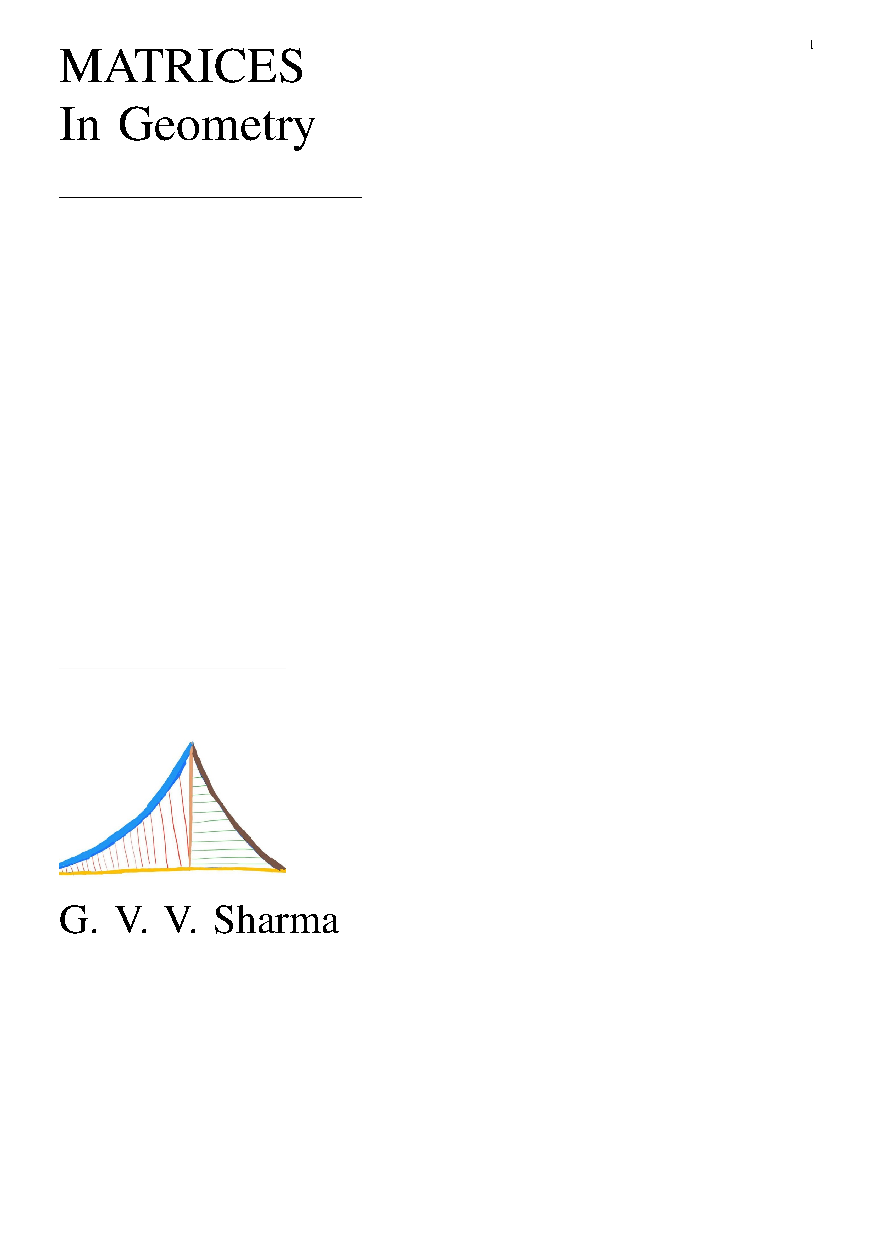
\includegraphics[width=0.75\columnwidth]{chapters/12/6/3/8/figs/main.png}
		\caption{}
		\label{fig:12/6/3/8}
  	\end{figure}
The equation of the conic can be represented as
\begin{align}
\vec{x}^{\top}\myvec{1&0\\0&0}\vec{x}+2\myvec{-2&\frac{-1}{2}}\vec{x}+4=0
\end{align}
So,
\begin{align}
\vec{V}=\myvec{1&0\\0&0},
\vec{u}^{\top}=\myvec{-2&\frac{-1}{2}},
f=4
\end{align}
The direction vector of the line passing through (2,0) and (4,4) is 
\begin{align}
\vec{m}=\myvec{1\\2}
\implies
\vec{n}=\myvec{2\\-1}.
\end{align}
The eigenvector corresponding to the zero eigenvalue is 
\begin{align}
\vec{p}_1=\myvec{0\\1},
\end{align}
In
\eqref{eq:conic_tangent_q_eigen},
\begin{align}
	\kappa=\frac{\myvec{0&1}\myvec{-2\\ \frac{-1}{2}}}{\myvec{0&1}\myvec{2\\-1}}
	=\frac{1}{2}
\end{align}
Substituting  $\kappa$,
from 
\eqref{eq:conic_tangent_q_eigen},
\begin{align}
	\myvec{\sbrak{\myvec{-2\\\frac{-1}{2}}+\frac{1}{2}\myvec{2\\-1}}^{\top} \\ \myvec{1&0\\0&0}}\vec{q} &= \myvec{-4 \\ \frac{1}{2}\myvec{2\\-1}-\myvec{-2\\\frac{-1}{2}}}\\
	\implies
	\myvec{-1&-1 \\ 1&0 \\ 0&0}\vec{q}&=\myvec{-4 \\ 3 \\ 0}
\end{align}
yielding
\begin{align}
\myvec{-1&-1 \\ 1&0}\vec{q} = \myvec{-4\\3}
\end{align}
The augmented matrix is 
\begin{align*}
  \myvec{
                -1&-1&\vrule&-4\\
	        1&0&\vrule&3}
  \xleftrightarrow[]{R_1 \leftarrow R_1+ 2R_2}
     \myvec{
	         1&-1&\vrule&2\\
	         1&0&\vrule&3}
      \\
 \xleftrightarrow[]{R_2 \leftarrow R_2 - R_1}
     \myvec{
	         1&-1&\vrule&2\\
	         0&1&\vrule&1}
 \xleftrightarrow[]{R_1 \leftarrow R_1 + R_2}
     \myvec{
	         1&0&\vrule&3\\
	         0&1&\vrule&1}
      \\ \implies \vec{q}=\myvec{3\\1}
\end{align*}
which is the desired 
point of contact.
See Fig. 
		\ref{fig:12/6/3/8}.



\iffalse
\latexprintindex
\fi

\end{document}


\item   Points $\vec{A}, \vec{B}, \vec{C}$ are defined to be collinear if 
		\begin{align}
			\label{eq:app-app-line-rank}
			\rank{\myvec{1 & 1 & 1 \\ \vec{A}& \vec{B}&\vec{C}}} = 2
		\end{align}
Are the given points in
			\eqref{eq:app-tri-pts}
collinear?
\\
\solution 
From 
			\eqref{eq:app-tri-pts},
\begin{align}
    \label{eq:app-1.1.3,2}
\myvec{
    1 & 1 & 1\\
    \vec{A} & \vec{B} & \vec{C} \\
    } 
    =
    %\label{eq:app-matthrowoperations}
    \myvec{
    1 & 1 & 1
    \\
    1 & -4 & -3
    \\
    -1 & 6 & -5
    }
     \xleftrightarrow[]{R_3 \leftarrow R_3+R_2}
    \myvec{
    1 & 1 & 1
    \\
    1 & -4 & -3
    \\
    0 & 2 & -8 
    }
    \\
     \xleftrightarrow[]{R_2\leftarrow R_1-R_2}
    \myvec{
    1 & 1 & 1
    \\
    0 & 5 & 4
    \\
    0 & 2 & -8 
    }
     \xleftrightarrow[]{R_3\leftarrow R_3-\frac{2}{5}R_2}
    \myvec{
    1 & 1 & 1
    \\
    0 & 5 & 4
    \\
    0 & 0 & \frac{-48}{5}
    }
\end{align}
There are no zero rows. So,
\begin{align}
    \text{rank}\myvec{
    1 & 1 & 1\\
    \vec{A} & \vec{B} & \vec{C} \\
    } &= 3 
\end{align}  
Hence,  the points $\vec{A},\vec{B},\vec{C}$ are not collinear. 
This is visible in 
\figref{fig1:Triangle}.
\begin{figure}[H]
\centering
\includegraphics[width=0.75\columnwidth]{figs/triangle/vector.pdf}
\caption{$\triangle ABC$}
\label{fig1:Triangle}
\end{figure}
% \\		\documentclass[journal]{IEEEtran}
\usepackage{gvv-book}
\usepackage{gvv}
%\usepackage{styles/front}
%\usepackage{Wiley-AuthoringTemplate}
%\usepackage[sectionbib,authoryear]{natbib}% for name-date citation comment the below line
%\usepackage[sectionbib,numbers]{natbib}% for numbered citation comment the above line

%%********************************************************************%%
%%       How many levels of section head would you like numbered?     %%
%% 0= no section numbers, 1= section, 2= section, 3= subsection %%
\setcounter{secnumdepth}{3}
%%********************************************************************%%
%%**********************************************************************%%
%%     How many levels of section head would you like to appear in the  %%
%%				Table of Contents?			%%
%% 0= chapter, 1= section, 2= section, 3= subsection titles.	%%
\setcounter{tocdepth}{2}
%%**********************************************************************%%

%\includeonly{ch01}
\makeindex

\begin{document}
\bibliographystyle{IEEEtran}
\onecolumn


\title{
	\begin{flushleft}
	MATRICES \\ In Geometry
	\\
\rule{0.4\columnwidth}{0.4pt}
\end{flushleft}
}
\author{
\vspace{7cm}
	\begin{flushleft}
\includegraphics[width=0.2\columnwidth]{figs/logo.jpg}
\\
		{	\huge G. V. V. Sharma}
		\\
\vspace{1cm}
https://creativecommons.org/licenses/by-sa/3.0/
\\
and
\\
https://www.gnu.org/licenses/fdl-1.3.en.html
	\end{flushleft}
%\IEEEpubid{\makebox[\columnwidth]{978-1-7281-5966-1/20/\$31.00 ©2020 IEEE \hfill} \hspace{\columnsep}\makebox[\columnwidth]{ }}
}
\maketitle

\newpage


\tableofcontents

\newpage
\twocolumn

%\section{Triangle}
\section{Vectors}
Consider a triangle with vertices
		\begin{align}
			\label{eq:tri-pts}
			\vec{A} = \myvec{1 \\ -1},\,
			\vec{B} = \myvec{-4 \\ 6},\,
			\vec{C} = \myvec{-3 \\ -5}
		\end{align}
\subsection{Sides}
%\renewcommand{\theequation}{\theenumi}
\begin{enumerate}[label=\thesubsection.\arabic*.,ref=\thesubsection.\theenumi]
%\numberwithin{equation}{enumi}
\item The direction vector of $AB$ is defined as
		\begin{align}
			\vec{B}-
			\vec{A}
		\end{align}
Find the direction vectors of $AB, BC$ and $CA$.
\\
\solution 
\begin{enumerate} 
\item  The Direction vector of $AB$ is 
	\begin{align}  \vec{B} - \vec{A} 
		=\myvec{ -4\\ 6 } - \myvec{ 1\\ -1 }
 = \myvec{ -4 - 1\\ 6 - (-1) } = \myvec{ -5\\ 7 }
		\label{eq:app-geo-dir-vec-ab}
 \end{align}
\item The Direction vector of $BC$ is
	\begin{align} \vec{C} - \vec{B}=\myvec{ -3\\ -5} - \myvec{ -4\\ 6 }
 = \myvec{ -3 - (-4)\\ -5 - 6 } = \myvec{1\\ -11 }
		\label{eq:app-geo-dir-vec-bc}
  \end{align}
  \item  The Direction vector of $CA$  is
	  \begin{align}  \vec{A} - \vec{C} =\myvec{ 1\\ -1 }-\myvec{ -3\\ -5}
 = \myvec{ 1 - (-3)\\ -1 - (-5) } = \myvec{ 4\\ 4 }
		\label{eq:app-geo-dir-vec-ca}
  \end{align}
 \end{enumerate}
%	\input{solutions/1/1/1/prob_1.tex}
	\item The length of side $BC$ is 
		\label{prob:side-length}
		\begin{align}
			c = \norm{\vec{B}-\vec{A}} \triangleq \sqrt{\brak{\vec{B}-\vec{A}}^{\top}\brak{\vec{B}-\vec{A}}}
		\end{align}
		where
		\begin{align}
			\vec{A}^{\top}\triangleq\myvec{1 & -1}
		\end{align}
		Similarly, 
		\begin{align}
b = \norm{\vec{C}-\vec{B}},\,
a = \norm{\vec{A}-\vec{C}}
		\end{align}
		Find $a, b, c$.
\begin{enumerate}
	\item 
	From 	
		\eqref{eq:app-geo-dir-vec-ab},
\begin{align}
\vec{A}-\vec{B} &= \myvec{5\\-7}, \\
\implies 	c &= 	\norm{\vec{B}-\vec{A}} = \norm{\vec{A}-\vec{B}} 
	\\
	&= \sqrt{\myvec{5 & -7}\myvec{5\\-7}}
= \sqrt{\brak{5}^2 +\brak{7}^2}\\
	&=\sqrt{74}
		\label{eq:app-geo-norm-ab}
\end{align}
	\item Similarly, from 
		\eqref{eq:app-geo-dir-vec-bc},
\begin{align}
	a &= \norm{\vec{B}-\vec{C}} 
	= \sqrt{\myvec{-1 & 11}\myvec{-1\\11}}
\\
&= \sqrt{\brak{1}^2+\brak{11}^2}
	= \sqrt{122}
		\label{eq:app-geo-norm-bc}
\end{align}
and
		from 		\eqref{eq:app-geo-dir-vec-ca},
	\item 
		\begin{align}
			b &= \norm{\vec{A}-\vec{C}} = \sqrt{\myvec{4 & 4}\myvec{4\\4}}
\\
&= \sqrt{\brak{4}^2+\brak{4}^2}
	=\sqrt{32}
		\label{eq:app-geo-norm-ca}
\end{align}
\end{enumerate}
%  \\            
  %\input{solutions/1/1/2a/main.tex}
\item   Points $\vec{A}, \vec{B}, \vec{C}$ are defined to be collinear if 
		\begin{align}
			\label{eq:app-app-line-rank}
			\rank{\myvec{1 & 1 & 1 \\ \vec{A}& \vec{B}&\vec{C}}} = 2
		\end{align}
Are the given points in
			\eqref{eq:app-tri-pts}
collinear?
\\
\solution 
From 
			\eqref{eq:app-tri-pts},
\begin{align}
    \label{eq:app-1.1.3,2}
\myvec{
    1 & 1 & 1\\
    \vec{A} & \vec{B} & \vec{C} \\
    } 
    =
    %\label{eq:app-matthrowoperations}
    \myvec{
    1 & 1 & 1
    \\
    1 & -4 & -3
    \\
    -1 & 6 & -5
    }
     \xleftrightarrow[]{R_3 \leftarrow R_3+R_2}
    \myvec{
    1 & 1 & 1
    \\
    1 & -4 & -3
    \\
    0 & 2 & -8 
    }
    \\
     \xleftrightarrow[]{R_2\leftarrow R_1-R_2}
    \myvec{
    1 & 1 & 1
    \\
    0 & 5 & 4
    \\
    0 & 2 & -8 
    }
     \xleftrightarrow[]{R_3\leftarrow R_3-\frac{2}{5}R_2}
    \myvec{
    1 & 1 & 1
    \\
    0 & 5 & 4
    \\
    0 & 0 & \frac{-48}{5}
    }
\end{align}
There are no zero rows. So,
\begin{align}
    \text{rank}\myvec{
    1 & 1 & 1\\
    \vec{A} & \vec{B} & \vec{C} \\
    } &= 3 
\end{align}  
Hence,  the points $\vec{A},\vec{B},\vec{C}$ are not collinear. 
This is visible in 
\figref{fig1:Triangle}.
\begin{figure}[H]
\centering
\includegraphics[width=0.75\columnwidth]{figs/triangle/vector.pdf}
\caption{$\triangle ABC$}
\label{fig1:Triangle}
\end{figure}
% \\		\input{solutions/1/1/3/main.tex}
\item The parameteric form of the equation  of $AB$ is 
		\begin{align}
			\label{eq:app-geo-param}
			\vec{x}=\vec{A}+k\vec{m} \quad k \ne 0,
		\end{align}
		where
		\begin{align}
\vec{m}=\vec{B}-\vec{A}
		\end{align}
is the direction vector of $AB$.
Find the parameteric equations of $AB, BC$ and $CA$.
\\
\solution
From 
			\eqref{eq:app-geo-param} and
		\eqref{eq:app-geo-dir-vec-ab},
the parametric equation for $AB$ is given by
\begin{align}
AB: \vec{x} = &\myvec{1\\-1} + k \myvec{-5\\7}
\end{align}
Similarly, from 
		\eqref{eq:app-geo-dir-vec-bc} and
		\eqref{eq:app-geo-dir-vec-ca},
\begin{align}
BC: \vec{x} = &\myvec{-4\\6} + k \myvec{1\\-11}\\
CA: \vec{x} = &\myvec{-3\\-5} + k \myvec{4\\4}
\end{align}

%		\input{solutions/1/1/4/main.tex}
\item The normal form of the equation of $AB$  is 
		\begin{align}
			\label{eq:app-geo-normal}
			\vec{n}^{\top}\brak{	\vec{x}-\vec{A}} = 0
		\end{align}
		where 
		\begin{align}
			\vec{n}^{\top}\vec{m}&=\vec{n}^{\top}\brak{\vec{B}-\vec{A}} = 0
			\\
			\text{or, } \vec{n}&=\myvec{0 & 1 \\ -1 & 0} \vec{m}
			\label{eq:app-geo-norm-vec}
		\end{align}
Find the normal form of the equations of $AB, BC$ and $CA$.
\\
\solution
\begin{enumerate}
	\item
From
		\eqref{eq:app-geo-dir-vec-bc}, 
the direction vector of side $\vec{BC}$ is
\begin{align}
\vec{m}
	&=\myvec{1\\-11}
	\\
\implies \vec{n} &= \myvec{0 & 1\\
  -1 & 0}\myvec{1\\-11}
 = \myvec{-11\\-1}
		\label{eq:app-geo-norm-vec-bc}
\end{align}
from 
			\eqref{eq:app-geo-norm-vec}.
Hence, from 
			\eqref{eq:app-geo-normal},
the normal equation of side $BC$ is 
\begin{align}
	\vec{n}^{\top}\brak{	\vec{x}-\vec{B}} &= 0
			\\
\implies    \myvec{-11 & -1}\vec{x}&=\myvec{-11 & -1}\myvec{-4\\6}\\
    \implies
BC: \quad    \myvec{11 & 1}\vec{x}&=-38
\end{align}
\item Similarly, for $AB$,
from 
		\eqref{eq:app-geo-dir-vec-ab}, 
\begin{align}
	\vec{m} &= \myvec{-5\\7}
	\\
\implies        \vec{n} 
                &= \myvec{0&1\\-1&0}\myvec{-5\\7}
                = \myvec{7\\5}
		\label{eq:app-geo-norm-vec-ab}
\end{align}
and 
\begin{align}
	\vec{n}^{\top}\brak{	\vec{x}-\vec{A}} &= 0
	\\
	\implies
                AB: \quad  \vec{n}^{\top}\vec{x} &= \myvec{7&5}\myvec{1\\-1}\\    
       \implies\myvec{7&5}\vec{x} &= 2
\end{align}
\item For 
$CA$, 
from 
		\eqref{eq:app-geo-dir-vec-ca}, 
\begin{align}
\vec{m} &= \myvec{1 \\ 1}
\\
		\label{eq:app-geo-norm-vec-ca}
\implies \vec{n} 
&= \myvec{0&1 \\ -1&0}\myvec{1 \\ 1}
= \myvec{1 \\ -1}\\
\\
\implies	\vec{n}^{\top}\brak{	\vec{x}-\vec{C}} &= 0
\\
\implies \myvec{1&-1}{\vec{x}} &= \myvec{1&-1}\myvec{-3 \\ -5} 
= 2 
\end{align}
\end{enumerate}

%\input{solutions/1/1/5/assign1.tex}
\item The area of $\triangle ABC$ is defined as
		\begin{align}
			\label{eq:app-tri-area-cross}
			\frac{1}{2}\norm{{\brak{\vec{A}-\vec{B}}\times \brak{\vec{A}-\vec{C}}}}
		\end{align}
		where
		\begin{align}
			\vec{A}\times\vec{B} \triangleq \mydet{1 & -4 \\-1 & 6}
		\end{align}
		Find the area of $\triangle ABC$.\\
\solution
From
		\eqref{eq:app-geo-dir-vec-ab}
		and
		\eqref{eq:app-geo-dir-vec-ca},
\begin{align}
	\vec{A}-\vec{B}=\myvec{5\\-7},
	\vec{A}-\vec{C}&=\myvec{4\\4}\\
\implies (\vec{A}-\vec{B})\times(\vec{A}-\vec{C}) &=\mydet{5 & 4\\-7 & 4}\\
&=5\times 4-4\times (-7)\\&=48\\
\implies\frac{1}{2}\norm{(\vec{A}-\vec{B})\times(\vec{A}-\vec{C})}&=\frac{48}{2}=24
\end{align}
which is the desired area.

%  		\input{solutions/1/1/6/main.tex}
	\item Find the angles $A, B, C$ if 
%    \label{prop:angle2d}
  \begin{align}
    \label{eq:app-angle2d}
			\cos A \triangleq 
\frac{\brak{\vec{B}-\vec{A}}^{\top}{\vec{C}-\vec{A}}}{\norm{\vec{B}-\vec{A}}\norm{\vec{C}-\vec{A}}}
  \end{align}\\
  \solution
\begin{enumerate}
	\item From 
		\eqref{eq:app-geo-dir-vec-ab},
		\eqref{eq:app-geo-dir-vec-ca},
		\eqref{eq:app-geo-norm-ab}
		and
		\eqref{eq:app-geo-norm-ca}
\begin{align}
	(\vec{B}-\vec{A})^{\top}(\vec{C}-\vec{A})&=\myvec{-5&7}\myvec{-4\\-4}\\
	&=-8
	\\
	\implies
	\cos{A}&= \frac{-8}{\sqrt{74} \sqrt{32}}
	= \frac{-1}{\sqrt{37}}\\
	\implies A&=\cos^{-1}{\frac{-1}{\sqrt{37}}}
\end{align}
	\item From 
		\eqref{eq:app-geo-dir-vec-ab},
		\eqref{eq:app-geo-dir-vec-bc},
		\eqref{eq:app-geo-norm-ab}
		and
		\eqref{eq:app-geo-norm-bc}
\begin{align}
	(\vec{C}-\vec{B})^{\top}(\vec{A}-\vec{B})&=\myvec{1&-11}\myvec{5\\-7}\\
	&= 82
	\\
	\implies
	\cos{B}&= \frac{82}{\sqrt{74} \sqrt{122}}
	= \frac{41}{\sqrt{2257}}\\
	\implies B&=\cos^{-1}{\frac{41}{\sqrt{2257}}}
\end{align}
	\item From 
		\eqref{eq:app-geo-dir-vec-bc},
		\eqref{eq:app-geo-dir-vec-ca},
		\eqref{eq:app-geo-norm-bc}
		and
		\eqref{eq:app-geo-norm-ca}
\begin{align}
	(\vec{A}-\vec{C})^{\top}(\vec{B}-\vec{C})&=\myvec{4&4}\myvec{-1\\11}\\
	&=40
	\\
\implies	\cos{C}&= \frac{40}{\sqrt{32} \sqrt{122}}
	= \frac{5}{\sqrt{61}}\\
	\implies C&=\cos^{-1}{\frac{5}{\sqrt{61}}}
\end{align}

\end{enumerate}
%  	\input{solutions/1/1/7/main.tex}
All codes for this section are available at
\begin{lstlisting}
	codes/triangle/sides.py
\end{lstlisting}
\end{enumerate}

\subsection{Median}
\input{chapters/triangle/median}
\subsection{Altitude}
\input{chapters/triangle/altitude}
\subsection{Perpendicular Bisector}
\input{chapters/triangle/perp-bisect}
\subsection{Angle Bisector}
\input{chapters/triangle/angle-bisect}
\subsection{Eigenvalues and Eigenvectors}
\input{chapters/triangle/eigen}
\section{Matrices}
The mid point of $PB$ is
\begin{align}
\vec{M} =\frac{1}{2}(\vec{P}+\vec{B})
	= \myvec{4 \\ -2}  
\end{align}
which is equal to the direction vector of $OM$.
\begin{align}
\because \vec{M} \equiv
	 \myvec{1 \\ -\frac{1}{2}},
	m = -\frac{1}{2}
\end{align}
which is the desired slope.
See 
		\figref{fig:11/10/1/5}.
	\begin{figure}[!ht]
		\centering
 \includegraphics[width=\columnwidth]{chapters/11/10/1/5/figs/line.png}
		\caption{}
		\label{fig:11/10/1/5}
  	\end{figure}


%\section{Quadrilateral}
%\input{./chapters/exercises/quad_geo_exer}

\appendices
\section{Tangents to a Circle}
\numberwithin{equation}{section}
	\begin{figure}[H]
		\centering
 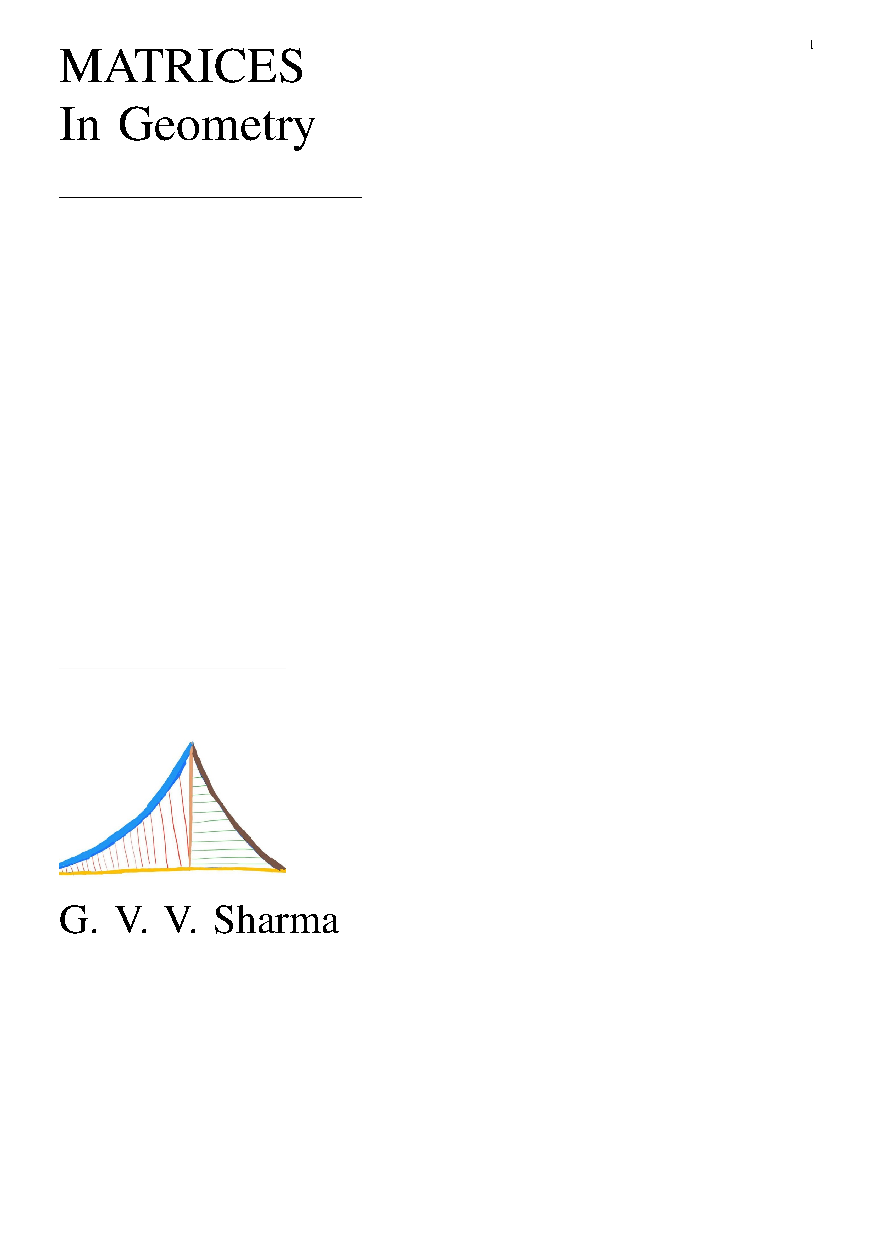
\includegraphics[width=0.75\columnwidth]{chapters/12/6/3/8/figs/main.png}
		\caption{}
		\label{fig:12/6/3/8}
  	\end{figure}
The equation of the conic can be represented as
\begin{align}
\vec{x}^{\top}\myvec{1&0\\0&0}\vec{x}+2\myvec{-2&\frac{-1}{2}}\vec{x}+4=0
\end{align}
So,
\begin{align}
\vec{V}=\myvec{1&0\\0&0},
\vec{u}^{\top}=\myvec{-2&\frac{-1}{2}},
f=4
\end{align}
The direction vector of the line passing through (2,0) and (4,4) is 
\begin{align}
\vec{m}=\myvec{1\\2}
\implies
\vec{n}=\myvec{2\\-1}.
\end{align}
The eigenvector corresponding to the zero eigenvalue is 
\begin{align}
\vec{p}_1=\myvec{0\\1},
\end{align}
In
\eqref{eq:conic_tangent_q_eigen},
\begin{align}
	\kappa=\frac{\myvec{0&1}\myvec{-2\\ \frac{-1}{2}}}{\myvec{0&1}\myvec{2\\-1}}
	=\frac{1}{2}
\end{align}
Substituting  $\kappa$,
from 
\eqref{eq:conic_tangent_q_eigen},
\begin{align}
	\myvec{\sbrak{\myvec{-2\\\frac{-1}{2}}+\frac{1}{2}\myvec{2\\-1}}^{\top} \\ \myvec{1&0\\0&0}}\vec{q} &= \myvec{-4 \\ \frac{1}{2}\myvec{2\\-1}-\myvec{-2\\\frac{-1}{2}}}\\
	\implies
	\myvec{-1&-1 \\ 1&0 \\ 0&0}\vec{q}&=\myvec{-4 \\ 3 \\ 0}
\end{align}
yielding
\begin{align}
\myvec{-1&-1 \\ 1&0}\vec{q} = \myvec{-4\\3}
\end{align}
The augmented matrix is 
\begin{align*}
  \myvec{
                -1&-1&\vrule&-4\\
	        1&0&\vrule&3}
  \xleftrightarrow[]{R_1 \leftarrow R_1+ 2R_2}
     \myvec{
	         1&-1&\vrule&2\\
	         1&0&\vrule&3}
      \\
 \xleftrightarrow[]{R_2 \leftarrow R_2 - R_1}
     \myvec{
	         1&-1&\vrule&2\\
	         0&1&\vrule&1}
 \xleftrightarrow[]{R_1 \leftarrow R_1 + R_2}
     \myvec{
	         1&0&\vrule&3\\
	         0&1&\vrule&1}
      \\ \implies \vec{q}=\myvec{3\\1}
\end{align*}
which is the desired 
point of contact.
See Fig. 
		\ref{fig:12/6/3/8}.



\iffalse
\latexprintindex
\fi

\end{document}


\item The parameteric form of the equation  of $AB$ is 
		\begin{align}
			\label{eq:app-geo-param}
			\vec{x}=\vec{A}+k\vec{m} \quad k \ne 0,
		\end{align}
		where
		\begin{align}
\vec{m}=\vec{B}-\vec{A}
		\end{align}
is the direction vector of $AB$.
Find the parameteric equations of $AB, BC$ and $CA$.
\\
\solution
From 
			\eqref{eq:app-geo-param} and
		\eqref{eq:app-geo-dir-vec-ab},
the parametric equation for $AB$ is given by
\begin{align}
AB: \vec{x} = &\myvec{1\\-1} + k \myvec{-5\\7}
\end{align}
Similarly, from 
		\eqref{eq:app-geo-dir-vec-bc} and
		\eqref{eq:app-geo-dir-vec-ca},
\begin{align}
BC: \vec{x} = &\myvec{-4\\6} + k \myvec{1\\-11}\\
CA: \vec{x} = &\myvec{-3\\-5} + k \myvec{4\\4}
\end{align}

%		\documentclass[journal]{IEEEtran}
\usepackage{gvv-book}
\usepackage{gvv}
%\usepackage{styles/front}
%\usepackage{Wiley-AuthoringTemplate}
%\usepackage[sectionbib,authoryear]{natbib}% for name-date citation comment the below line
%\usepackage[sectionbib,numbers]{natbib}% for numbered citation comment the above line

%%********************************************************************%%
%%       How many levels of section head would you like numbered?     %%
%% 0= no section numbers, 1= section, 2= section, 3= subsection %%
\setcounter{secnumdepth}{3}
%%********************************************************************%%
%%**********************************************************************%%
%%     How many levels of section head would you like to appear in the  %%
%%				Table of Contents?			%%
%% 0= chapter, 1= section, 2= section, 3= subsection titles.	%%
\setcounter{tocdepth}{2}
%%**********************************************************************%%

%\includeonly{ch01}
\makeindex

\begin{document}
\bibliographystyle{IEEEtran}
\onecolumn


\title{
	\begin{flushleft}
	MATRICES \\ In Geometry
	\\
\rule{0.4\columnwidth}{0.4pt}
\end{flushleft}
}
\author{
\vspace{7cm}
	\begin{flushleft}
\includegraphics[width=0.2\columnwidth]{figs/logo.jpg}
\\
		{	\huge G. V. V. Sharma}
		\\
\vspace{1cm}
https://creativecommons.org/licenses/by-sa/3.0/
\\
and
\\
https://www.gnu.org/licenses/fdl-1.3.en.html
	\end{flushleft}
%\IEEEpubid{\makebox[\columnwidth]{978-1-7281-5966-1/20/\$31.00 ©2020 IEEE \hfill} \hspace{\columnsep}\makebox[\columnwidth]{ }}
}
\maketitle

\newpage


\tableofcontents

\newpage
\twocolumn

%\section{Triangle}
\section{Vectors}
Consider a triangle with vertices
		\begin{align}
			\label{eq:tri-pts}
			\vec{A} = \myvec{1 \\ -1},\,
			\vec{B} = \myvec{-4 \\ 6},\,
			\vec{C} = \myvec{-3 \\ -5}
		\end{align}
\subsection{Sides}
%\renewcommand{\theequation}{\theenumi}
\begin{enumerate}[label=\thesubsection.\arabic*.,ref=\thesubsection.\theenumi]
%\numberwithin{equation}{enumi}
\item The direction vector of $AB$ is defined as
		\begin{align}
			\vec{B}-
			\vec{A}
		\end{align}
Find the direction vectors of $AB, BC$ and $CA$.
\\
\solution 
\begin{enumerate} 
\item  The Direction vector of $AB$ is 
	\begin{align}  \vec{B} - \vec{A} 
		=\myvec{ -4\\ 6 } - \myvec{ 1\\ -1 }
 = \myvec{ -4 - 1\\ 6 - (-1) } = \myvec{ -5\\ 7 }
		\label{eq:app-geo-dir-vec-ab}
 \end{align}
\item The Direction vector of $BC$ is
	\begin{align} \vec{C} - \vec{B}=\myvec{ -3\\ -5} - \myvec{ -4\\ 6 }
 = \myvec{ -3 - (-4)\\ -5 - 6 } = \myvec{1\\ -11 }
		\label{eq:app-geo-dir-vec-bc}
  \end{align}
  \item  The Direction vector of $CA$  is
	  \begin{align}  \vec{A} - \vec{C} =\myvec{ 1\\ -1 }-\myvec{ -3\\ -5}
 = \myvec{ 1 - (-3)\\ -1 - (-5) } = \myvec{ 4\\ 4 }
		\label{eq:app-geo-dir-vec-ca}
  \end{align}
 \end{enumerate}
%	\input{solutions/1/1/1/prob_1.tex}
	\item The length of side $BC$ is 
		\label{prob:side-length}
		\begin{align}
			c = \norm{\vec{B}-\vec{A}} \triangleq \sqrt{\brak{\vec{B}-\vec{A}}^{\top}\brak{\vec{B}-\vec{A}}}
		\end{align}
		where
		\begin{align}
			\vec{A}^{\top}\triangleq\myvec{1 & -1}
		\end{align}
		Similarly, 
		\begin{align}
b = \norm{\vec{C}-\vec{B}},\,
a = \norm{\vec{A}-\vec{C}}
		\end{align}
		Find $a, b, c$.
\begin{enumerate}
	\item 
	From 	
		\eqref{eq:app-geo-dir-vec-ab},
\begin{align}
\vec{A}-\vec{B} &= \myvec{5\\-7}, \\
\implies 	c &= 	\norm{\vec{B}-\vec{A}} = \norm{\vec{A}-\vec{B}} 
	\\
	&= \sqrt{\myvec{5 & -7}\myvec{5\\-7}}
= \sqrt{\brak{5}^2 +\brak{7}^2}\\
	&=\sqrt{74}
		\label{eq:app-geo-norm-ab}
\end{align}
	\item Similarly, from 
		\eqref{eq:app-geo-dir-vec-bc},
\begin{align}
	a &= \norm{\vec{B}-\vec{C}} 
	= \sqrt{\myvec{-1 & 11}\myvec{-1\\11}}
\\
&= \sqrt{\brak{1}^2+\brak{11}^2}
	= \sqrt{122}
		\label{eq:app-geo-norm-bc}
\end{align}
and
		from 		\eqref{eq:app-geo-dir-vec-ca},
	\item 
		\begin{align}
			b &= \norm{\vec{A}-\vec{C}} = \sqrt{\myvec{4 & 4}\myvec{4\\4}}
\\
&= \sqrt{\brak{4}^2+\brak{4}^2}
	=\sqrt{32}
		\label{eq:app-geo-norm-ca}
\end{align}
\end{enumerate}
%  \\            
  %\input{solutions/1/1/2a/main.tex}
\item   Points $\vec{A}, \vec{B}, \vec{C}$ are defined to be collinear if 
		\begin{align}
			\label{eq:app-app-line-rank}
			\rank{\myvec{1 & 1 & 1 \\ \vec{A}& \vec{B}&\vec{C}}} = 2
		\end{align}
Are the given points in
			\eqref{eq:app-tri-pts}
collinear?
\\
\solution 
From 
			\eqref{eq:app-tri-pts},
\begin{align}
    \label{eq:app-1.1.3,2}
\myvec{
    1 & 1 & 1\\
    \vec{A} & \vec{B} & \vec{C} \\
    } 
    =
    %\label{eq:app-matthrowoperations}
    \myvec{
    1 & 1 & 1
    \\
    1 & -4 & -3
    \\
    -1 & 6 & -5
    }
     \xleftrightarrow[]{R_3 \leftarrow R_3+R_2}
    \myvec{
    1 & 1 & 1
    \\
    1 & -4 & -3
    \\
    0 & 2 & -8 
    }
    \\
     \xleftrightarrow[]{R_2\leftarrow R_1-R_2}
    \myvec{
    1 & 1 & 1
    \\
    0 & 5 & 4
    \\
    0 & 2 & -8 
    }
     \xleftrightarrow[]{R_3\leftarrow R_3-\frac{2}{5}R_2}
    \myvec{
    1 & 1 & 1
    \\
    0 & 5 & 4
    \\
    0 & 0 & \frac{-48}{5}
    }
\end{align}
There are no zero rows. So,
\begin{align}
    \text{rank}\myvec{
    1 & 1 & 1\\
    \vec{A} & \vec{B} & \vec{C} \\
    } &= 3 
\end{align}  
Hence,  the points $\vec{A},\vec{B},\vec{C}$ are not collinear. 
This is visible in 
\figref{fig1:Triangle}.
\begin{figure}[H]
\centering
\includegraphics[width=0.75\columnwidth]{figs/triangle/vector.pdf}
\caption{$\triangle ABC$}
\label{fig1:Triangle}
\end{figure}
% \\		\input{solutions/1/1/3/main.tex}
\item The parameteric form of the equation  of $AB$ is 
		\begin{align}
			\label{eq:app-geo-param}
			\vec{x}=\vec{A}+k\vec{m} \quad k \ne 0,
		\end{align}
		where
		\begin{align}
\vec{m}=\vec{B}-\vec{A}
		\end{align}
is the direction vector of $AB$.
Find the parameteric equations of $AB, BC$ and $CA$.
\\
\solution
From 
			\eqref{eq:app-geo-param} and
		\eqref{eq:app-geo-dir-vec-ab},
the parametric equation for $AB$ is given by
\begin{align}
AB: \vec{x} = &\myvec{1\\-1} + k \myvec{-5\\7}
\end{align}
Similarly, from 
		\eqref{eq:app-geo-dir-vec-bc} and
		\eqref{eq:app-geo-dir-vec-ca},
\begin{align}
BC: \vec{x} = &\myvec{-4\\6} + k \myvec{1\\-11}\\
CA: \vec{x} = &\myvec{-3\\-5} + k \myvec{4\\4}
\end{align}

%		\input{solutions/1/1/4/main.tex}
\item The normal form of the equation of $AB$  is 
		\begin{align}
			\label{eq:app-geo-normal}
			\vec{n}^{\top}\brak{	\vec{x}-\vec{A}} = 0
		\end{align}
		where 
		\begin{align}
			\vec{n}^{\top}\vec{m}&=\vec{n}^{\top}\brak{\vec{B}-\vec{A}} = 0
			\\
			\text{or, } \vec{n}&=\myvec{0 & 1 \\ -1 & 0} \vec{m}
			\label{eq:app-geo-norm-vec}
		\end{align}
Find the normal form of the equations of $AB, BC$ and $CA$.
\\
\solution
\begin{enumerate}
	\item
From
		\eqref{eq:app-geo-dir-vec-bc}, 
the direction vector of side $\vec{BC}$ is
\begin{align}
\vec{m}
	&=\myvec{1\\-11}
	\\
\implies \vec{n} &= \myvec{0 & 1\\
  -1 & 0}\myvec{1\\-11}
 = \myvec{-11\\-1}
		\label{eq:app-geo-norm-vec-bc}
\end{align}
from 
			\eqref{eq:app-geo-norm-vec}.
Hence, from 
			\eqref{eq:app-geo-normal},
the normal equation of side $BC$ is 
\begin{align}
	\vec{n}^{\top}\brak{	\vec{x}-\vec{B}} &= 0
			\\
\implies    \myvec{-11 & -1}\vec{x}&=\myvec{-11 & -1}\myvec{-4\\6}\\
    \implies
BC: \quad    \myvec{11 & 1}\vec{x}&=-38
\end{align}
\item Similarly, for $AB$,
from 
		\eqref{eq:app-geo-dir-vec-ab}, 
\begin{align}
	\vec{m} &= \myvec{-5\\7}
	\\
\implies        \vec{n} 
                &= \myvec{0&1\\-1&0}\myvec{-5\\7}
                = \myvec{7\\5}
		\label{eq:app-geo-norm-vec-ab}
\end{align}
and 
\begin{align}
	\vec{n}^{\top}\brak{	\vec{x}-\vec{A}} &= 0
	\\
	\implies
                AB: \quad  \vec{n}^{\top}\vec{x} &= \myvec{7&5}\myvec{1\\-1}\\    
       \implies\myvec{7&5}\vec{x} &= 2
\end{align}
\item For 
$CA$, 
from 
		\eqref{eq:app-geo-dir-vec-ca}, 
\begin{align}
\vec{m} &= \myvec{1 \\ 1}
\\
		\label{eq:app-geo-norm-vec-ca}
\implies \vec{n} 
&= \myvec{0&1 \\ -1&0}\myvec{1 \\ 1}
= \myvec{1 \\ -1}\\
\\
\implies	\vec{n}^{\top}\brak{	\vec{x}-\vec{C}} &= 0
\\
\implies \myvec{1&-1}{\vec{x}} &= \myvec{1&-1}\myvec{-3 \\ -5} 
= 2 
\end{align}
\end{enumerate}

%\input{solutions/1/1/5/assign1.tex}
\item The area of $\triangle ABC$ is defined as
		\begin{align}
			\label{eq:app-tri-area-cross}
			\frac{1}{2}\norm{{\brak{\vec{A}-\vec{B}}\times \brak{\vec{A}-\vec{C}}}}
		\end{align}
		where
		\begin{align}
			\vec{A}\times\vec{B} \triangleq \mydet{1 & -4 \\-1 & 6}
		\end{align}
		Find the area of $\triangle ABC$.\\
\solution
From
		\eqref{eq:app-geo-dir-vec-ab}
		and
		\eqref{eq:app-geo-dir-vec-ca},
\begin{align}
	\vec{A}-\vec{B}=\myvec{5\\-7},
	\vec{A}-\vec{C}&=\myvec{4\\4}\\
\implies (\vec{A}-\vec{B})\times(\vec{A}-\vec{C}) &=\mydet{5 & 4\\-7 & 4}\\
&=5\times 4-4\times (-7)\\&=48\\
\implies\frac{1}{2}\norm{(\vec{A}-\vec{B})\times(\vec{A}-\vec{C})}&=\frac{48}{2}=24
\end{align}
which is the desired area.

%  		\input{solutions/1/1/6/main.tex}
	\item Find the angles $A, B, C$ if 
%    \label{prop:angle2d}
  \begin{align}
    \label{eq:app-angle2d}
			\cos A \triangleq 
\frac{\brak{\vec{B}-\vec{A}}^{\top}{\vec{C}-\vec{A}}}{\norm{\vec{B}-\vec{A}}\norm{\vec{C}-\vec{A}}}
  \end{align}\\
  \solution
\begin{enumerate}
	\item From 
		\eqref{eq:app-geo-dir-vec-ab},
		\eqref{eq:app-geo-dir-vec-ca},
		\eqref{eq:app-geo-norm-ab}
		and
		\eqref{eq:app-geo-norm-ca}
\begin{align}
	(\vec{B}-\vec{A})^{\top}(\vec{C}-\vec{A})&=\myvec{-5&7}\myvec{-4\\-4}\\
	&=-8
	\\
	\implies
	\cos{A}&= \frac{-8}{\sqrt{74} \sqrt{32}}
	= \frac{-1}{\sqrt{37}}\\
	\implies A&=\cos^{-1}{\frac{-1}{\sqrt{37}}}
\end{align}
	\item From 
		\eqref{eq:app-geo-dir-vec-ab},
		\eqref{eq:app-geo-dir-vec-bc},
		\eqref{eq:app-geo-norm-ab}
		and
		\eqref{eq:app-geo-norm-bc}
\begin{align}
	(\vec{C}-\vec{B})^{\top}(\vec{A}-\vec{B})&=\myvec{1&-11}\myvec{5\\-7}\\
	&= 82
	\\
	\implies
	\cos{B}&= \frac{82}{\sqrt{74} \sqrt{122}}
	= \frac{41}{\sqrt{2257}}\\
	\implies B&=\cos^{-1}{\frac{41}{\sqrt{2257}}}
\end{align}
	\item From 
		\eqref{eq:app-geo-dir-vec-bc},
		\eqref{eq:app-geo-dir-vec-ca},
		\eqref{eq:app-geo-norm-bc}
		and
		\eqref{eq:app-geo-norm-ca}
\begin{align}
	(\vec{A}-\vec{C})^{\top}(\vec{B}-\vec{C})&=\myvec{4&4}\myvec{-1\\11}\\
	&=40
	\\
\implies	\cos{C}&= \frac{40}{\sqrt{32} \sqrt{122}}
	= \frac{5}{\sqrt{61}}\\
	\implies C&=\cos^{-1}{\frac{5}{\sqrt{61}}}
\end{align}

\end{enumerate}
%  	\input{solutions/1/1/7/main.tex}
All codes for this section are available at
\begin{lstlisting}
	codes/triangle/sides.py
\end{lstlisting}
\end{enumerate}

\subsection{Median}
\input{chapters/triangle/median}
\subsection{Altitude}
\input{chapters/triangle/altitude}
\subsection{Perpendicular Bisector}
\input{chapters/triangle/perp-bisect}
\subsection{Angle Bisector}
\input{chapters/triangle/angle-bisect}
\subsection{Eigenvalues and Eigenvectors}
\input{chapters/triangle/eigen}
\section{Matrices}
The mid point of $PB$ is
\begin{align}
\vec{M} =\frac{1}{2}(\vec{P}+\vec{B})
	= \myvec{4 \\ -2}  
\end{align}
which is equal to the direction vector of $OM$.
\begin{align}
\because \vec{M} \equiv
	 \myvec{1 \\ -\frac{1}{2}},
	m = -\frac{1}{2}
\end{align}
which is the desired slope.
See 
		\figref{fig:11/10/1/5}.
	\begin{figure}[!ht]
		\centering
 \includegraphics[width=\columnwidth]{chapters/11/10/1/5/figs/line.png}
		\caption{}
		\label{fig:11/10/1/5}
  	\end{figure}


%\section{Quadrilateral}
%\input{./chapters/exercises/quad_geo_exer}

\appendices
\section{Tangents to a Circle}
\numberwithin{equation}{section}
	\begin{figure}[H]
		\centering
 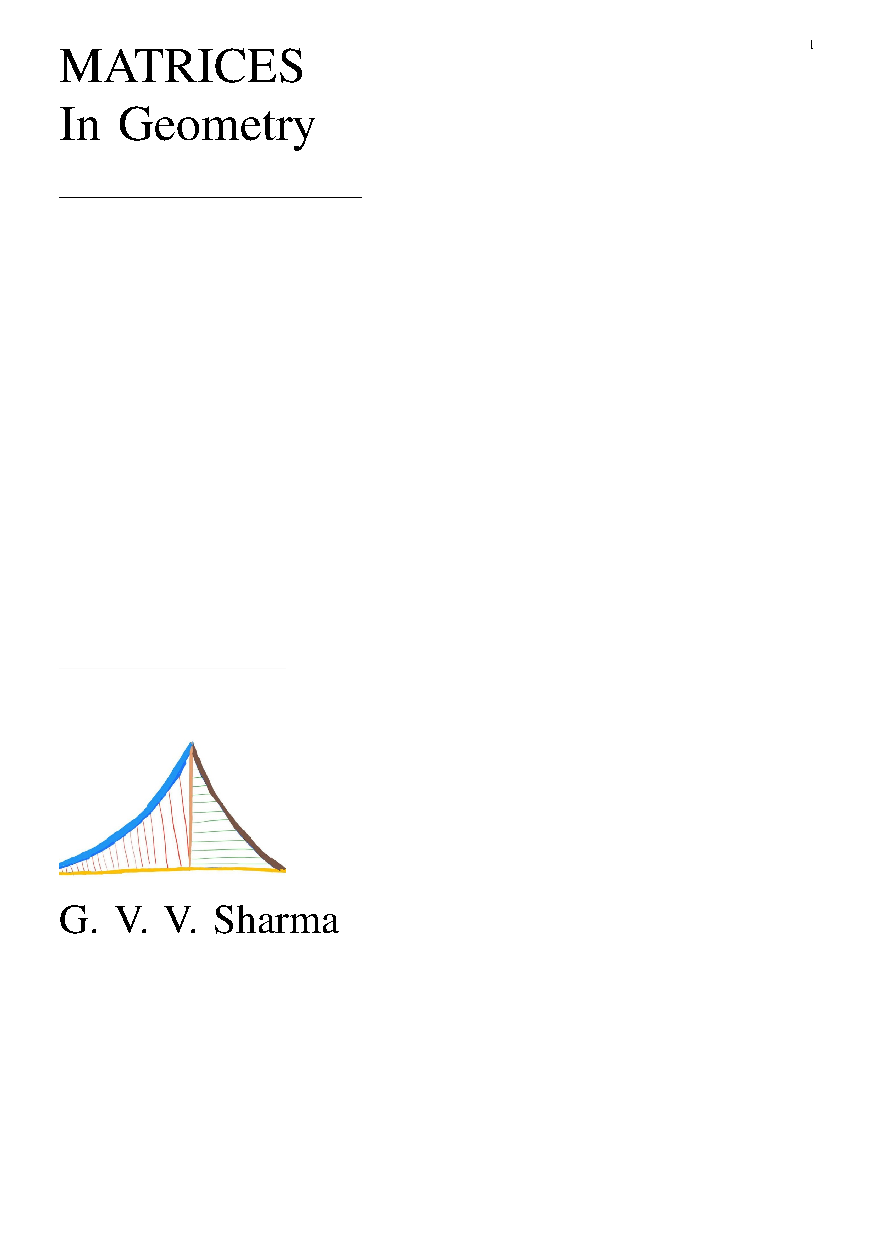
\includegraphics[width=0.75\columnwidth]{chapters/12/6/3/8/figs/main.png}
		\caption{}
		\label{fig:12/6/3/8}
  	\end{figure}
The equation of the conic can be represented as
\begin{align}
\vec{x}^{\top}\myvec{1&0\\0&0}\vec{x}+2\myvec{-2&\frac{-1}{2}}\vec{x}+4=0
\end{align}
So,
\begin{align}
\vec{V}=\myvec{1&0\\0&0},
\vec{u}^{\top}=\myvec{-2&\frac{-1}{2}},
f=4
\end{align}
The direction vector of the line passing through (2,0) and (4,4) is 
\begin{align}
\vec{m}=\myvec{1\\2}
\implies
\vec{n}=\myvec{2\\-1}.
\end{align}
The eigenvector corresponding to the zero eigenvalue is 
\begin{align}
\vec{p}_1=\myvec{0\\1},
\end{align}
In
\eqref{eq:conic_tangent_q_eigen},
\begin{align}
	\kappa=\frac{\myvec{0&1}\myvec{-2\\ \frac{-1}{2}}}{\myvec{0&1}\myvec{2\\-1}}
	=\frac{1}{2}
\end{align}
Substituting  $\kappa$,
from 
\eqref{eq:conic_tangent_q_eigen},
\begin{align}
	\myvec{\sbrak{\myvec{-2\\\frac{-1}{2}}+\frac{1}{2}\myvec{2\\-1}}^{\top} \\ \myvec{1&0\\0&0}}\vec{q} &= \myvec{-4 \\ \frac{1}{2}\myvec{2\\-1}-\myvec{-2\\\frac{-1}{2}}}\\
	\implies
	\myvec{-1&-1 \\ 1&0 \\ 0&0}\vec{q}&=\myvec{-4 \\ 3 \\ 0}
\end{align}
yielding
\begin{align}
\myvec{-1&-1 \\ 1&0}\vec{q} = \myvec{-4\\3}
\end{align}
The augmented matrix is 
\begin{align*}
  \myvec{
                -1&-1&\vrule&-4\\
	        1&0&\vrule&3}
  \xleftrightarrow[]{R_1 \leftarrow R_1+ 2R_2}
     \myvec{
	         1&-1&\vrule&2\\
	         1&0&\vrule&3}
      \\
 \xleftrightarrow[]{R_2 \leftarrow R_2 - R_1}
     \myvec{
	         1&-1&\vrule&2\\
	         0&1&\vrule&1}
 \xleftrightarrow[]{R_1 \leftarrow R_1 + R_2}
     \myvec{
	         1&0&\vrule&3\\
	         0&1&\vrule&1}
      \\ \implies \vec{q}=\myvec{3\\1}
\end{align*}
which is the desired 
point of contact.
See Fig. 
		\ref{fig:12/6/3/8}.



\iffalse
\latexprintindex
\fi

\end{document}


\item The normal form of the equation of $AB$  is 
		\begin{align}
			\label{eq:app-geo-normal}
			\vec{n}^{\top}\brak{	\vec{x}-\vec{A}} = 0
		\end{align}
		where 
		\begin{align}
			\vec{n}^{\top}\vec{m}&=\vec{n}^{\top}\brak{\vec{B}-\vec{A}} = 0
			\\
			\text{or, } \vec{n}&=\myvec{0 & 1 \\ -1 & 0} \vec{m}
			\label{eq:app-geo-norm-vec}
		\end{align}
Find the normal form of the equations of $AB, BC$ and $CA$.
\\
\solution
\begin{enumerate}
	\item
From
		\eqref{eq:app-geo-dir-vec-bc}, 
the direction vector of side $\vec{BC}$ is
\begin{align}
\vec{m}
	&=\myvec{1\\-11}
	\\
\implies \vec{n} &= \myvec{0 & 1\\
  -1 & 0}\myvec{1\\-11}
 = \myvec{-11\\-1}
		\label{eq:app-geo-norm-vec-bc}
\end{align}
from 
			\eqref{eq:app-geo-norm-vec}.
Hence, from 
			\eqref{eq:app-geo-normal},
the normal equation of side $BC$ is 
\begin{align}
	\vec{n}^{\top}\brak{	\vec{x}-\vec{B}} &= 0
			\\
\implies    \myvec{-11 & -1}\vec{x}&=\myvec{-11 & -1}\myvec{-4\\6}\\
    \implies
BC: \quad    \myvec{11 & 1}\vec{x}&=-38
\end{align}
\item Similarly, for $AB$,
from 
		\eqref{eq:app-geo-dir-vec-ab}, 
\begin{align}
	\vec{m} &= \myvec{-5\\7}
	\\
\implies        \vec{n} 
                &= \myvec{0&1\\-1&0}\myvec{-5\\7}
                = \myvec{7\\5}
		\label{eq:app-geo-norm-vec-ab}
\end{align}
and 
\begin{align}
	\vec{n}^{\top}\brak{	\vec{x}-\vec{A}} &= 0
	\\
	\implies
                AB: \quad  \vec{n}^{\top}\vec{x} &= \myvec{7&5}\myvec{1\\-1}\\    
       \implies\myvec{7&5}\vec{x} &= 2
\end{align}
\item For 
$CA$, 
from 
		\eqref{eq:app-geo-dir-vec-ca}, 
\begin{align}
\vec{m} &= \myvec{1 \\ 1}
\\
		\label{eq:app-geo-norm-vec-ca}
\implies \vec{n} 
&= \myvec{0&1 \\ -1&0}\myvec{1 \\ 1}
= \myvec{1 \\ -1}\\
\\
\implies	\vec{n}^{\top}\brak{	\vec{x}-\vec{C}} &= 0
\\
\implies \myvec{1&-1}{\vec{x}} &= \myvec{1&-1}\myvec{-3 \\ -5} 
= 2 
\end{align}
\end{enumerate}

%\input{solutions/1/1/5/assign1.tex}
\item The area of $\triangle ABC$ is defined as
		\begin{align}
			\label{eq:app-tri-area-cross}
			\frac{1}{2}\norm{{\brak{\vec{A}-\vec{B}}\times \brak{\vec{A}-\vec{C}}}}
		\end{align}
		where
		\begin{align}
			\vec{A}\times\vec{B} \triangleq \mydet{1 & -4 \\-1 & 6}
		\end{align}
		Find the area of $\triangle ABC$.\\
\solution
From
		\eqref{eq:app-geo-dir-vec-ab}
		and
		\eqref{eq:app-geo-dir-vec-ca},
\begin{align}
	\vec{A}-\vec{B}=\myvec{5\\-7},
	\vec{A}-\vec{C}&=\myvec{4\\4}\\
\implies (\vec{A}-\vec{B})\times(\vec{A}-\vec{C}) &=\mydet{5 & 4\\-7 & 4}\\
&=5\times 4-4\times (-7)\\&=48\\
\implies\frac{1}{2}\norm{(\vec{A}-\vec{B})\times(\vec{A}-\vec{C})}&=\frac{48}{2}=24
\end{align}
which is the desired area.

%  		\documentclass[journal]{IEEEtran}
\usepackage{gvv-book}
\usepackage{gvv}
%\usepackage{styles/front}
%\usepackage{Wiley-AuthoringTemplate}
%\usepackage[sectionbib,authoryear]{natbib}% for name-date citation comment the below line
%\usepackage[sectionbib,numbers]{natbib}% for numbered citation comment the above line

%%********************************************************************%%
%%       How many levels of section head would you like numbered?     %%
%% 0= no section numbers, 1= section, 2= section, 3= subsection %%
\setcounter{secnumdepth}{3}
%%********************************************************************%%
%%**********************************************************************%%
%%     How many levels of section head would you like to appear in the  %%
%%				Table of Contents?			%%
%% 0= chapter, 1= section, 2= section, 3= subsection titles.	%%
\setcounter{tocdepth}{2}
%%**********************************************************************%%

%\includeonly{ch01}
\makeindex

\begin{document}
\bibliographystyle{IEEEtran}
\onecolumn


\title{
	\begin{flushleft}
	MATRICES \\ In Geometry
	\\
\rule{0.4\columnwidth}{0.4pt}
\end{flushleft}
}
\author{
\vspace{7cm}
	\begin{flushleft}
\includegraphics[width=0.2\columnwidth]{figs/logo.jpg}
\\
		{	\huge G. V. V. Sharma}
		\\
\vspace{1cm}
https://creativecommons.org/licenses/by-sa/3.0/
\\
and
\\
https://www.gnu.org/licenses/fdl-1.3.en.html
	\end{flushleft}
%\IEEEpubid{\makebox[\columnwidth]{978-1-7281-5966-1/20/\$31.00 ©2020 IEEE \hfill} \hspace{\columnsep}\makebox[\columnwidth]{ }}
}
\maketitle

\newpage


\tableofcontents

\newpage
\twocolumn

%\section{Triangle}
\section{Vectors}
Consider a triangle with vertices
		\begin{align}
			\label{eq:tri-pts}
			\vec{A} = \myvec{1 \\ -1},\,
			\vec{B} = \myvec{-4 \\ 6},\,
			\vec{C} = \myvec{-3 \\ -5}
		\end{align}
\subsection{Sides}
%\renewcommand{\theequation}{\theenumi}
\begin{enumerate}[label=\thesubsection.\arabic*.,ref=\thesubsection.\theenumi]
%\numberwithin{equation}{enumi}
\item The direction vector of $AB$ is defined as
		\begin{align}
			\vec{B}-
			\vec{A}
		\end{align}
Find the direction vectors of $AB, BC$ and $CA$.
\\
\solution 
\begin{enumerate} 
\item  The Direction vector of $AB$ is 
	\begin{align}  \vec{B} - \vec{A} 
		=\myvec{ -4\\ 6 } - \myvec{ 1\\ -1 }
 = \myvec{ -4 - 1\\ 6 - (-1) } = \myvec{ -5\\ 7 }
		\label{eq:app-geo-dir-vec-ab}
 \end{align}
\item The Direction vector of $BC$ is
	\begin{align} \vec{C} - \vec{B}=\myvec{ -3\\ -5} - \myvec{ -4\\ 6 }
 = \myvec{ -3 - (-4)\\ -5 - 6 } = \myvec{1\\ -11 }
		\label{eq:app-geo-dir-vec-bc}
  \end{align}
  \item  The Direction vector of $CA$  is
	  \begin{align}  \vec{A} - \vec{C} =\myvec{ 1\\ -1 }-\myvec{ -3\\ -5}
 = \myvec{ 1 - (-3)\\ -1 - (-5) } = \myvec{ 4\\ 4 }
		\label{eq:app-geo-dir-vec-ca}
  \end{align}
 \end{enumerate}
%	\input{solutions/1/1/1/prob_1.tex}
	\item The length of side $BC$ is 
		\label{prob:side-length}
		\begin{align}
			c = \norm{\vec{B}-\vec{A}} \triangleq \sqrt{\brak{\vec{B}-\vec{A}}^{\top}\brak{\vec{B}-\vec{A}}}
		\end{align}
		where
		\begin{align}
			\vec{A}^{\top}\triangleq\myvec{1 & -1}
		\end{align}
		Similarly, 
		\begin{align}
b = \norm{\vec{C}-\vec{B}},\,
a = \norm{\vec{A}-\vec{C}}
		\end{align}
		Find $a, b, c$.
\begin{enumerate}
	\item 
	From 	
		\eqref{eq:app-geo-dir-vec-ab},
\begin{align}
\vec{A}-\vec{B} &= \myvec{5\\-7}, \\
\implies 	c &= 	\norm{\vec{B}-\vec{A}} = \norm{\vec{A}-\vec{B}} 
	\\
	&= \sqrt{\myvec{5 & -7}\myvec{5\\-7}}
= \sqrt{\brak{5}^2 +\brak{7}^2}\\
	&=\sqrt{74}
		\label{eq:app-geo-norm-ab}
\end{align}
	\item Similarly, from 
		\eqref{eq:app-geo-dir-vec-bc},
\begin{align}
	a &= \norm{\vec{B}-\vec{C}} 
	= \sqrt{\myvec{-1 & 11}\myvec{-1\\11}}
\\
&= \sqrt{\brak{1}^2+\brak{11}^2}
	= \sqrt{122}
		\label{eq:app-geo-norm-bc}
\end{align}
and
		from 		\eqref{eq:app-geo-dir-vec-ca},
	\item 
		\begin{align}
			b &= \norm{\vec{A}-\vec{C}} = \sqrt{\myvec{4 & 4}\myvec{4\\4}}
\\
&= \sqrt{\brak{4}^2+\brak{4}^2}
	=\sqrt{32}
		\label{eq:app-geo-norm-ca}
\end{align}
\end{enumerate}
%  \\            
  %\input{solutions/1/1/2a/main.tex}
\item   Points $\vec{A}, \vec{B}, \vec{C}$ are defined to be collinear if 
		\begin{align}
			\label{eq:app-app-line-rank}
			\rank{\myvec{1 & 1 & 1 \\ \vec{A}& \vec{B}&\vec{C}}} = 2
		\end{align}
Are the given points in
			\eqref{eq:app-tri-pts}
collinear?
\\
\solution 
From 
			\eqref{eq:app-tri-pts},
\begin{align}
    \label{eq:app-1.1.3,2}
\myvec{
    1 & 1 & 1\\
    \vec{A} & \vec{B} & \vec{C} \\
    } 
    =
    %\label{eq:app-matthrowoperations}
    \myvec{
    1 & 1 & 1
    \\
    1 & -4 & -3
    \\
    -1 & 6 & -5
    }
     \xleftrightarrow[]{R_3 \leftarrow R_3+R_2}
    \myvec{
    1 & 1 & 1
    \\
    1 & -4 & -3
    \\
    0 & 2 & -8 
    }
    \\
     \xleftrightarrow[]{R_2\leftarrow R_1-R_2}
    \myvec{
    1 & 1 & 1
    \\
    0 & 5 & 4
    \\
    0 & 2 & -8 
    }
     \xleftrightarrow[]{R_3\leftarrow R_3-\frac{2}{5}R_2}
    \myvec{
    1 & 1 & 1
    \\
    0 & 5 & 4
    \\
    0 & 0 & \frac{-48}{5}
    }
\end{align}
There are no zero rows. So,
\begin{align}
    \text{rank}\myvec{
    1 & 1 & 1\\
    \vec{A} & \vec{B} & \vec{C} \\
    } &= 3 
\end{align}  
Hence,  the points $\vec{A},\vec{B},\vec{C}$ are not collinear. 
This is visible in 
\figref{fig1:Triangle}.
\begin{figure}[H]
\centering
\includegraphics[width=0.75\columnwidth]{figs/triangle/vector.pdf}
\caption{$\triangle ABC$}
\label{fig1:Triangle}
\end{figure}
% \\		\input{solutions/1/1/3/main.tex}
\item The parameteric form of the equation  of $AB$ is 
		\begin{align}
			\label{eq:app-geo-param}
			\vec{x}=\vec{A}+k\vec{m} \quad k \ne 0,
		\end{align}
		where
		\begin{align}
\vec{m}=\vec{B}-\vec{A}
		\end{align}
is the direction vector of $AB$.
Find the parameteric equations of $AB, BC$ and $CA$.
\\
\solution
From 
			\eqref{eq:app-geo-param} and
		\eqref{eq:app-geo-dir-vec-ab},
the parametric equation for $AB$ is given by
\begin{align}
AB: \vec{x} = &\myvec{1\\-1} + k \myvec{-5\\7}
\end{align}
Similarly, from 
		\eqref{eq:app-geo-dir-vec-bc} and
		\eqref{eq:app-geo-dir-vec-ca},
\begin{align}
BC: \vec{x} = &\myvec{-4\\6} + k \myvec{1\\-11}\\
CA: \vec{x} = &\myvec{-3\\-5} + k \myvec{4\\4}
\end{align}

%		\input{solutions/1/1/4/main.tex}
\item The normal form of the equation of $AB$  is 
		\begin{align}
			\label{eq:app-geo-normal}
			\vec{n}^{\top}\brak{	\vec{x}-\vec{A}} = 0
		\end{align}
		where 
		\begin{align}
			\vec{n}^{\top}\vec{m}&=\vec{n}^{\top}\brak{\vec{B}-\vec{A}} = 0
			\\
			\text{or, } \vec{n}&=\myvec{0 & 1 \\ -1 & 0} \vec{m}
			\label{eq:app-geo-norm-vec}
		\end{align}
Find the normal form of the equations of $AB, BC$ and $CA$.
\\
\solution
\begin{enumerate}
	\item
From
		\eqref{eq:app-geo-dir-vec-bc}, 
the direction vector of side $\vec{BC}$ is
\begin{align}
\vec{m}
	&=\myvec{1\\-11}
	\\
\implies \vec{n} &= \myvec{0 & 1\\
  -1 & 0}\myvec{1\\-11}
 = \myvec{-11\\-1}
		\label{eq:app-geo-norm-vec-bc}
\end{align}
from 
			\eqref{eq:app-geo-norm-vec}.
Hence, from 
			\eqref{eq:app-geo-normal},
the normal equation of side $BC$ is 
\begin{align}
	\vec{n}^{\top}\brak{	\vec{x}-\vec{B}} &= 0
			\\
\implies    \myvec{-11 & -1}\vec{x}&=\myvec{-11 & -1}\myvec{-4\\6}\\
    \implies
BC: \quad    \myvec{11 & 1}\vec{x}&=-38
\end{align}
\item Similarly, for $AB$,
from 
		\eqref{eq:app-geo-dir-vec-ab}, 
\begin{align}
	\vec{m} &= \myvec{-5\\7}
	\\
\implies        \vec{n} 
                &= \myvec{0&1\\-1&0}\myvec{-5\\7}
                = \myvec{7\\5}
		\label{eq:app-geo-norm-vec-ab}
\end{align}
and 
\begin{align}
	\vec{n}^{\top}\brak{	\vec{x}-\vec{A}} &= 0
	\\
	\implies
                AB: \quad  \vec{n}^{\top}\vec{x} &= \myvec{7&5}\myvec{1\\-1}\\    
       \implies\myvec{7&5}\vec{x} &= 2
\end{align}
\item For 
$CA$, 
from 
		\eqref{eq:app-geo-dir-vec-ca}, 
\begin{align}
\vec{m} &= \myvec{1 \\ 1}
\\
		\label{eq:app-geo-norm-vec-ca}
\implies \vec{n} 
&= \myvec{0&1 \\ -1&0}\myvec{1 \\ 1}
= \myvec{1 \\ -1}\\
\\
\implies	\vec{n}^{\top}\brak{	\vec{x}-\vec{C}} &= 0
\\
\implies \myvec{1&-1}{\vec{x}} &= \myvec{1&-1}\myvec{-3 \\ -5} 
= 2 
\end{align}
\end{enumerate}

%\input{solutions/1/1/5/assign1.tex}
\item The area of $\triangle ABC$ is defined as
		\begin{align}
			\label{eq:app-tri-area-cross}
			\frac{1}{2}\norm{{\brak{\vec{A}-\vec{B}}\times \brak{\vec{A}-\vec{C}}}}
		\end{align}
		where
		\begin{align}
			\vec{A}\times\vec{B} \triangleq \mydet{1 & -4 \\-1 & 6}
		\end{align}
		Find the area of $\triangle ABC$.\\
\solution
From
		\eqref{eq:app-geo-dir-vec-ab}
		and
		\eqref{eq:app-geo-dir-vec-ca},
\begin{align}
	\vec{A}-\vec{B}=\myvec{5\\-7},
	\vec{A}-\vec{C}&=\myvec{4\\4}\\
\implies (\vec{A}-\vec{B})\times(\vec{A}-\vec{C}) &=\mydet{5 & 4\\-7 & 4}\\
&=5\times 4-4\times (-7)\\&=48\\
\implies\frac{1}{2}\norm{(\vec{A}-\vec{B})\times(\vec{A}-\vec{C})}&=\frac{48}{2}=24
\end{align}
which is the desired area.

%  		\input{solutions/1/1/6/main.tex}
	\item Find the angles $A, B, C$ if 
%    \label{prop:angle2d}
  \begin{align}
    \label{eq:app-angle2d}
			\cos A \triangleq 
\frac{\brak{\vec{B}-\vec{A}}^{\top}{\vec{C}-\vec{A}}}{\norm{\vec{B}-\vec{A}}\norm{\vec{C}-\vec{A}}}
  \end{align}\\
  \solution
\begin{enumerate}
	\item From 
		\eqref{eq:app-geo-dir-vec-ab},
		\eqref{eq:app-geo-dir-vec-ca},
		\eqref{eq:app-geo-norm-ab}
		and
		\eqref{eq:app-geo-norm-ca}
\begin{align}
	(\vec{B}-\vec{A})^{\top}(\vec{C}-\vec{A})&=\myvec{-5&7}\myvec{-4\\-4}\\
	&=-8
	\\
	\implies
	\cos{A}&= \frac{-8}{\sqrt{74} \sqrt{32}}
	= \frac{-1}{\sqrt{37}}\\
	\implies A&=\cos^{-1}{\frac{-1}{\sqrt{37}}}
\end{align}
	\item From 
		\eqref{eq:app-geo-dir-vec-ab},
		\eqref{eq:app-geo-dir-vec-bc},
		\eqref{eq:app-geo-norm-ab}
		and
		\eqref{eq:app-geo-norm-bc}
\begin{align}
	(\vec{C}-\vec{B})^{\top}(\vec{A}-\vec{B})&=\myvec{1&-11}\myvec{5\\-7}\\
	&= 82
	\\
	\implies
	\cos{B}&= \frac{82}{\sqrt{74} \sqrt{122}}
	= \frac{41}{\sqrt{2257}}\\
	\implies B&=\cos^{-1}{\frac{41}{\sqrt{2257}}}
\end{align}
	\item From 
		\eqref{eq:app-geo-dir-vec-bc},
		\eqref{eq:app-geo-dir-vec-ca},
		\eqref{eq:app-geo-norm-bc}
		and
		\eqref{eq:app-geo-norm-ca}
\begin{align}
	(\vec{A}-\vec{C})^{\top}(\vec{B}-\vec{C})&=\myvec{4&4}\myvec{-1\\11}\\
	&=40
	\\
\implies	\cos{C}&= \frac{40}{\sqrt{32} \sqrt{122}}
	= \frac{5}{\sqrt{61}}\\
	\implies C&=\cos^{-1}{\frac{5}{\sqrt{61}}}
\end{align}

\end{enumerate}
%  	\input{solutions/1/1/7/main.tex}
All codes for this section are available at
\begin{lstlisting}
	codes/triangle/sides.py
\end{lstlisting}
\end{enumerate}

\subsection{Median}
\input{chapters/triangle/median}
\subsection{Altitude}
\input{chapters/triangle/altitude}
\subsection{Perpendicular Bisector}
\input{chapters/triangle/perp-bisect}
\subsection{Angle Bisector}
\input{chapters/triangle/angle-bisect}
\subsection{Eigenvalues and Eigenvectors}
\input{chapters/triangle/eigen}
\section{Matrices}
The mid point of $PB$ is
\begin{align}
\vec{M} =\frac{1}{2}(\vec{P}+\vec{B})
	= \myvec{4 \\ -2}  
\end{align}
which is equal to the direction vector of $OM$.
\begin{align}
\because \vec{M} \equiv
	 \myvec{1 \\ -\frac{1}{2}},
	m = -\frac{1}{2}
\end{align}
which is the desired slope.
See 
		\figref{fig:11/10/1/5}.
	\begin{figure}[!ht]
		\centering
 \includegraphics[width=\columnwidth]{chapters/11/10/1/5/figs/line.png}
		\caption{}
		\label{fig:11/10/1/5}
  	\end{figure}


%\section{Quadrilateral}
%\input{./chapters/exercises/quad_geo_exer}

\appendices
\section{Tangents to a Circle}
\numberwithin{equation}{section}
	\begin{figure}[H]
		\centering
 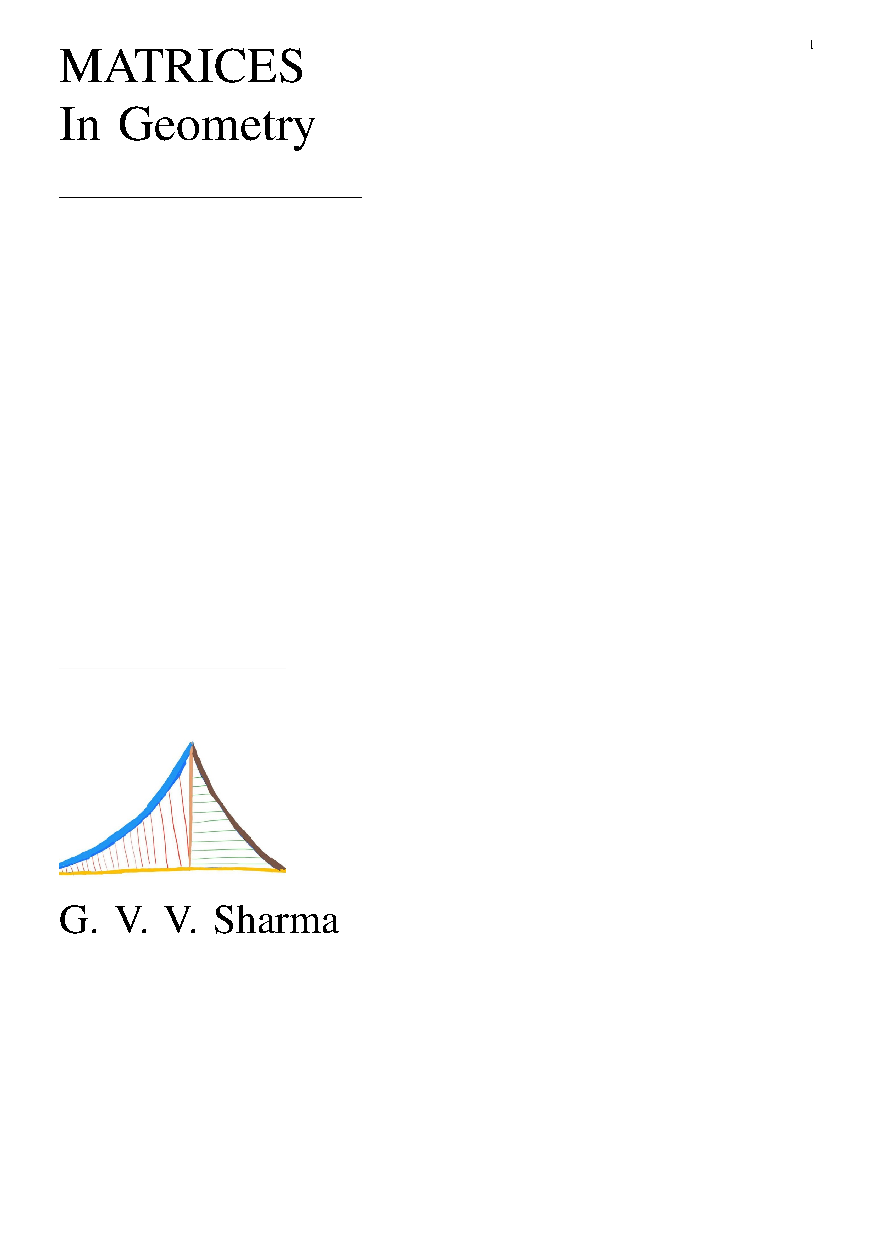
\includegraphics[width=0.75\columnwidth]{chapters/12/6/3/8/figs/main.png}
		\caption{}
		\label{fig:12/6/3/8}
  	\end{figure}
The equation of the conic can be represented as
\begin{align}
\vec{x}^{\top}\myvec{1&0\\0&0}\vec{x}+2\myvec{-2&\frac{-1}{2}}\vec{x}+4=0
\end{align}
So,
\begin{align}
\vec{V}=\myvec{1&0\\0&0},
\vec{u}^{\top}=\myvec{-2&\frac{-1}{2}},
f=4
\end{align}
The direction vector of the line passing through (2,0) and (4,4) is 
\begin{align}
\vec{m}=\myvec{1\\2}
\implies
\vec{n}=\myvec{2\\-1}.
\end{align}
The eigenvector corresponding to the zero eigenvalue is 
\begin{align}
\vec{p}_1=\myvec{0\\1},
\end{align}
In
\eqref{eq:conic_tangent_q_eigen},
\begin{align}
	\kappa=\frac{\myvec{0&1}\myvec{-2\\ \frac{-1}{2}}}{\myvec{0&1}\myvec{2\\-1}}
	=\frac{1}{2}
\end{align}
Substituting  $\kappa$,
from 
\eqref{eq:conic_tangent_q_eigen},
\begin{align}
	\myvec{\sbrak{\myvec{-2\\\frac{-1}{2}}+\frac{1}{2}\myvec{2\\-1}}^{\top} \\ \myvec{1&0\\0&0}}\vec{q} &= \myvec{-4 \\ \frac{1}{2}\myvec{2\\-1}-\myvec{-2\\\frac{-1}{2}}}\\
	\implies
	\myvec{-1&-1 \\ 1&0 \\ 0&0}\vec{q}&=\myvec{-4 \\ 3 \\ 0}
\end{align}
yielding
\begin{align}
\myvec{-1&-1 \\ 1&0}\vec{q} = \myvec{-4\\3}
\end{align}
The augmented matrix is 
\begin{align*}
  \myvec{
                -1&-1&\vrule&-4\\
	        1&0&\vrule&3}
  \xleftrightarrow[]{R_1 \leftarrow R_1+ 2R_2}
     \myvec{
	         1&-1&\vrule&2\\
	         1&0&\vrule&3}
      \\
 \xleftrightarrow[]{R_2 \leftarrow R_2 - R_1}
     \myvec{
	         1&-1&\vrule&2\\
	         0&1&\vrule&1}
 \xleftrightarrow[]{R_1 \leftarrow R_1 + R_2}
     \myvec{
	         1&0&\vrule&3\\
	         0&1&\vrule&1}
      \\ \implies \vec{q}=\myvec{3\\1}
\end{align*}
which is the desired 
point of contact.
See Fig. 
		\ref{fig:12/6/3/8}.



\iffalse
\latexprintindex
\fi

\end{document}


	\item Find the angles $A, B, C$ if 
%    \label{prop:angle2d}
  \begin{align}
    \label{eq:app-angle2d}
			\cos A \triangleq 
\frac{\brak{\vec{B}-\vec{A}}^{\top}{\vec{C}-\vec{A}}}{\norm{\vec{B}-\vec{A}}\norm{\vec{C}-\vec{A}}}
  \end{align}\\
  \solution
\begin{enumerate}
	\item From 
		\eqref{eq:app-geo-dir-vec-ab},
		\eqref{eq:app-geo-dir-vec-ca},
		\eqref{eq:app-geo-norm-ab}
		and
		\eqref{eq:app-geo-norm-ca}
\begin{align}
	(\vec{B}-\vec{A})^{\top}(\vec{C}-\vec{A})&=\myvec{-5&7}\myvec{-4\\-4}\\
	&=-8
	\\
	\implies
	\cos{A}&= \frac{-8}{\sqrt{74} \sqrt{32}}
	= \frac{-1}{\sqrt{37}}\\
	\implies A&=\cos^{-1}{\frac{-1}{\sqrt{37}}}
\end{align}
	\item From 
		\eqref{eq:app-geo-dir-vec-ab},
		\eqref{eq:app-geo-dir-vec-bc},
		\eqref{eq:app-geo-norm-ab}
		and
		\eqref{eq:app-geo-norm-bc}
\begin{align}
	(\vec{C}-\vec{B})^{\top}(\vec{A}-\vec{B})&=\myvec{1&-11}\myvec{5\\-7}\\
	&= 82
	\\
	\implies
	\cos{B}&= \frac{82}{\sqrt{74} \sqrt{122}}
	= \frac{41}{\sqrt{2257}}\\
	\implies B&=\cos^{-1}{\frac{41}{\sqrt{2257}}}
\end{align}
	\item From 
		\eqref{eq:app-geo-dir-vec-bc},
		\eqref{eq:app-geo-dir-vec-ca},
		\eqref{eq:app-geo-norm-bc}
		and
		\eqref{eq:app-geo-norm-ca}
\begin{align}
	(\vec{A}-\vec{C})^{\top}(\vec{B}-\vec{C})&=\myvec{4&4}\myvec{-1\\11}\\
	&=40
	\\
\implies	\cos{C}&= \frac{40}{\sqrt{32} \sqrt{122}}
	= \frac{5}{\sqrt{61}}\\
	\implies C&=\cos^{-1}{\frac{5}{\sqrt{61}}}
\end{align}

\end{enumerate}
%  	\documentclass[journal]{IEEEtran}
\usepackage{gvv-book}
\usepackage{gvv}
%\usepackage{styles/front}
%\usepackage{Wiley-AuthoringTemplate}
%\usepackage[sectionbib,authoryear]{natbib}% for name-date citation comment the below line
%\usepackage[sectionbib,numbers]{natbib}% for numbered citation comment the above line

%%********************************************************************%%
%%       How many levels of section head would you like numbered?     %%
%% 0= no section numbers, 1= section, 2= section, 3= subsection %%
\setcounter{secnumdepth}{3}
%%********************************************************************%%
%%**********************************************************************%%
%%     How many levels of section head would you like to appear in the  %%
%%				Table of Contents?			%%
%% 0= chapter, 1= section, 2= section, 3= subsection titles.	%%
\setcounter{tocdepth}{2}
%%**********************************************************************%%

%\includeonly{ch01}
\makeindex

\begin{document}
\bibliographystyle{IEEEtran}
\onecolumn


\title{
	\begin{flushleft}
	MATRICES \\ In Geometry
	\\
\rule{0.4\columnwidth}{0.4pt}
\end{flushleft}
}
\author{
\vspace{7cm}
	\begin{flushleft}
\includegraphics[width=0.2\columnwidth]{figs/logo.jpg}
\\
		{	\huge G. V. V. Sharma}
		\\
\vspace{1cm}
https://creativecommons.org/licenses/by-sa/3.0/
\\
and
\\
https://www.gnu.org/licenses/fdl-1.3.en.html
	\end{flushleft}
%\IEEEpubid{\makebox[\columnwidth]{978-1-7281-5966-1/20/\$31.00 ©2020 IEEE \hfill} \hspace{\columnsep}\makebox[\columnwidth]{ }}
}
\maketitle

\newpage


\tableofcontents

\newpage
\twocolumn

%\section{Triangle}
\section{Vectors}
Consider a triangle with vertices
		\begin{align}
			\label{eq:tri-pts}
			\vec{A} = \myvec{1 \\ -1},\,
			\vec{B} = \myvec{-4 \\ 6},\,
			\vec{C} = \myvec{-3 \\ -5}
		\end{align}
\subsection{Sides}
%\renewcommand{\theequation}{\theenumi}
\begin{enumerate}[label=\thesubsection.\arabic*.,ref=\thesubsection.\theenumi]
%\numberwithin{equation}{enumi}
\item The direction vector of $AB$ is defined as
		\begin{align}
			\vec{B}-
			\vec{A}
		\end{align}
Find the direction vectors of $AB, BC$ and $CA$.
\\
\solution 
\begin{enumerate} 
\item  The Direction vector of $AB$ is 
	\begin{align}  \vec{B} - \vec{A} 
		=\myvec{ -4\\ 6 } - \myvec{ 1\\ -1 }
 = \myvec{ -4 - 1\\ 6 - (-1) } = \myvec{ -5\\ 7 }
		\label{eq:app-geo-dir-vec-ab}
 \end{align}
\item The Direction vector of $BC$ is
	\begin{align} \vec{C} - \vec{B}=\myvec{ -3\\ -5} - \myvec{ -4\\ 6 }
 = \myvec{ -3 - (-4)\\ -5 - 6 } = \myvec{1\\ -11 }
		\label{eq:app-geo-dir-vec-bc}
  \end{align}
  \item  The Direction vector of $CA$  is
	  \begin{align}  \vec{A} - \vec{C} =\myvec{ 1\\ -1 }-\myvec{ -3\\ -5}
 = \myvec{ 1 - (-3)\\ -1 - (-5) } = \myvec{ 4\\ 4 }
		\label{eq:app-geo-dir-vec-ca}
  \end{align}
 \end{enumerate}
%	\input{solutions/1/1/1/prob_1.tex}
	\item The length of side $BC$ is 
		\label{prob:side-length}
		\begin{align}
			c = \norm{\vec{B}-\vec{A}} \triangleq \sqrt{\brak{\vec{B}-\vec{A}}^{\top}\brak{\vec{B}-\vec{A}}}
		\end{align}
		where
		\begin{align}
			\vec{A}^{\top}\triangleq\myvec{1 & -1}
		\end{align}
		Similarly, 
		\begin{align}
b = \norm{\vec{C}-\vec{B}},\,
a = \norm{\vec{A}-\vec{C}}
		\end{align}
		Find $a, b, c$.
\begin{enumerate}
	\item 
	From 	
		\eqref{eq:app-geo-dir-vec-ab},
\begin{align}
\vec{A}-\vec{B} &= \myvec{5\\-7}, \\
\implies 	c &= 	\norm{\vec{B}-\vec{A}} = \norm{\vec{A}-\vec{B}} 
	\\
	&= \sqrt{\myvec{5 & -7}\myvec{5\\-7}}
= \sqrt{\brak{5}^2 +\brak{7}^2}\\
	&=\sqrt{74}
		\label{eq:app-geo-norm-ab}
\end{align}
	\item Similarly, from 
		\eqref{eq:app-geo-dir-vec-bc},
\begin{align}
	a &= \norm{\vec{B}-\vec{C}} 
	= \sqrt{\myvec{-1 & 11}\myvec{-1\\11}}
\\
&= \sqrt{\brak{1}^2+\brak{11}^2}
	= \sqrt{122}
		\label{eq:app-geo-norm-bc}
\end{align}
and
		from 		\eqref{eq:app-geo-dir-vec-ca},
	\item 
		\begin{align}
			b &= \norm{\vec{A}-\vec{C}} = \sqrt{\myvec{4 & 4}\myvec{4\\4}}
\\
&= \sqrt{\brak{4}^2+\brak{4}^2}
	=\sqrt{32}
		\label{eq:app-geo-norm-ca}
\end{align}
\end{enumerate}
%  \\            
  %\input{solutions/1/1/2a/main.tex}
\item   Points $\vec{A}, \vec{B}, \vec{C}$ are defined to be collinear if 
		\begin{align}
			\label{eq:app-app-line-rank}
			\rank{\myvec{1 & 1 & 1 \\ \vec{A}& \vec{B}&\vec{C}}} = 2
		\end{align}
Are the given points in
			\eqref{eq:app-tri-pts}
collinear?
\\
\solution 
From 
			\eqref{eq:app-tri-pts},
\begin{align}
    \label{eq:app-1.1.3,2}
\myvec{
    1 & 1 & 1\\
    \vec{A} & \vec{B} & \vec{C} \\
    } 
    =
    %\label{eq:app-matthrowoperations}
    \myvec{
    1 & 1 & 1
    \\
    1 & -4 & -3
    \\
    -1 & 6 & -5
    }
     \xleftrightarrow[]{R_3 \leftarrow R_3+R_2}
    \myvec{
    1 & 1 & 1
    \\
    1 & -4 & -3
    \\
    0 & 2 & -8 
    }
    \\
     \xleftrightarrow[]{R_2\leftarrow R_1-R_2}
    \myvec{
    1 & 1 & 1
    \\
    0 & 5 & 4
    \\
    0 & 2 & -8 
    }
     \xleftrightarrow[]{R_3\leftarrow R_3-\frac{2}{5}R_2}
    \myvec{
    1 & 1 & 1
    \\
    0 & 5 & 4
    \\
    0 & 0 & \frac{-48}{5}
    }
\end{align}
There are no zero rows. So,
\begin{align}
    \text{rank}\myvec{
    1 & 1 & 1\\
    \vec{A} & \vec{B} & \vec{C} \\
    } &= 3 
\end{align}  
Hence,  the points $\vec{A},\vec{B},\vec{C}$ are not collinear. 
This is visible in 
\figref{fig1:Triangle}.
\begin{figure}[H]
\centering
\includegraphics[width=0.75\columnwidth]{figs/triangle/vector.pdf}
\caption{$\triangle ABC$}
\label{fig1:Triangle}
\end{figure}
% \\		\input{solutions/1/1/3/main.tex}
\item The parameteric form of the equation  of $AB$ is 
		\begin{align}
			\label{eq:app-geo-param}
			\vec{x}=\vec{A}+k\vec{m} \quad k \ne 0,
		\end{align}
		where
		\begin{align}
\vec{m}=\vec{B}-\vec{A}
		\end{align}
is the direction vector of $AB$.
Find the parameteric equations of $AB, BC$ and $CA$.
\\
\solution
From 
			\eqref{eq:app-geo-param} and
		\eqref{eq:app-geo-dir-vec-ab},
the parametric equation for $AB$ is given by
\begin{align}
AB: \vec{x} = &\myvec{1\\-1} + k \myvec{-5\\7}
\end{align}
Similarly, from 
		\eqref{eq:app-geo-dir-vec-bc} and
		\eqref{eq:app-geo-dir-vec-ca},
\begin{align}
BC: \vec{x} = &\myvec{-4\\6} + k \myvec{1\\-11}\\
CA: \vec{x} = &\myvec{-3\\-5} + k \myvec{4\\4}
\end{align}

%		\input{solutions/1/1/4/main.tex}
\item The normal form of the equation of $AB$  is 
		\begin{align}
			\label{eq:app-geo-normal}
			\vec{n}^{\top}\brak{	\vec{x}-\vec{A}} = 0
		\end{align}
		where 
		\begin{align}
			\vec{n}^{\top}\vec{m}&=\vec{n}^{\top}\brak{\vec{B}-\vec{A}} = 0
			\\
			\text{or, } \vec{n}&=\myvec{0 & 1 \\ -1 & 0} \vec{m}
			\label{eq:app-geo-norm-vec}
		\end{align}
Find the normal form of the equations of $AB, BC$ and $CA$.
\\
\solution
\begin{enumerate}
	\item
From
		\eqref{eq:app-geo-dir-vec-bc}, 
the direction vector of side $\vec{BC}$ is
\begin{align}
\vec{m}
	&=\myvec{1\\-11}
	\\
\implies \vec{n} &= \myvec{0 & 1\\
  -1 & 0}\myvec{1\\-11}
 = \myvec{-11\\-1}
		\label{eq:app-geo-norm-vec-bc}
\end{align}
from 
			\eqref{eq:app-geo-norm-vec}.
Hence, from 
			\eqref{eq:app-geo-normal},
the normal equation of side $BC$ is 
\begin{align}
	\vec{n}^{\top}\brak{	\vec{x}-\vec{B}} &= 0
			\\
\implies    \myvec{-11 & -1}\vec{x}&=\myvec{-11 & -1}\myvec{-4\\6}\\
    \implies
BC: \quad    \myvec{11 & 1}\vec{x}&=-38
\end{align}
\item Similarly, for $AB$,
from 
		\eqref{eq:app-geo-dir-vec-ab}, 
\begin{align}
	\vec{m} &= \myvec{-5\\7}
	\\
\implies        \vec{n} 
                &= \myvec{0&1\\-1&0}\myvec{-5\\7}
                = \myvec{7\\5}
		\label{eq:app-geo-norm-vec-ab}
\end{align}
and 
\begin{align}
	\vec{n}^{\top}\brak{	\vec{x}-\vec{A}} &= 0
	\\
	\implies
                AB: \quad  \vec{n}^{\top}\vec{x} &= \myvec{7&5}\myvec{1\\-1}\\    
       \implies\myvec{7&5}\vec{x} &= 2
\end{align}
\item For 
$CA$, 
from 
		\eqref{eq:app-geo-dir-vec-ca}, 
\begin{align}
\vec{m} &= \myvec{1 \\ 1}
\\
		\label{eq:app-geo-norm-vec-ca}
\implies \vec{n} 
&= \myvec{0&1 \\ -1&0}\myvec{1 \\ 1}
= \myvec{1 \\ -1}\\
\\
\implies	\vec{n}^{\top}\brak{	\vec{x}-\vec{C}} &= 0
\\
\implies \myvec{1&-1}{\vec{x}} &= \myvec{1&-1}\myvec{-3 \\ -5} 
= 2 
\end{align}
\end{enumerate}

%\input{solutions/1/1/5/assign1.tex}
\item The area of $\triangle ABC$ is defined as
		\begin{align}
			\label{eq:app-tri-area-cross}
			\frac{1}{2}\norm{{\brak{\vec{A}-\vec{B}}\times \brak{\vec{A}-\vec{C}}}}
		\end{align}
		where
		\begin{align}
			\vec{A}\times\vec{B} \triangleq \mydet{1 & -4 \\-1 & 6}
		\end{align}
		Find the area of $\triangle ABC$.\\
\solution
From
		\eqref{eq:app-geo-dir-vec-ab}
		and
		\eqref{eq:app-geo-dir-vec-ca},
\begin{align}
	\vec{A}-\vec{B}=\myvec{5\\-7},
	\vec{A}-\vec{C}&=\myvec{4\\4}\\
\implies (\vec{A}-\vec{B})\times(\vec{A}-\vec{C}) &=\mydet{5 & 4\\-7 & 4}\\
&=5\times 4-4\times (-7)\\&=48\\
\implies\frac{1}{2}\norm{(\vec{A}-\vec{B})\times(\vec{A}-\vec{C})}&=\frac{48}{2}=24
\end{align}
which is the desired area.

%  		\input{solutions/1/1/6/main.tex}
	\item Find the angles $A, B, C$ if 
%    \label{prop:angle2d}
  \begin{align}
    \label{eq:app-angle2d}
			\cos A \triangleq 
\frac{\brak{\vec{B}-\vec{A}}^{\top}{\vec{C}-\vec{A}}}{\norm{\vec{B}-\vec{A}}\norm{\vec{C}-\vec{A}}}
  \end{align}\\
  \solution
\begin{enumerate}
	\item From 
		\eqref{eq:app-geo-dir-vec-ab},
		\eqref{eq:app-geo-dir-vec-ca},
		\eqref{eq:app-geo-norm-ab}
		and
		\eqref{eq:app-geo-norm-ca}
\begin{align}
	(\vec{B}-\vec{A})^{\top}(\vec{C}-\vec{A})&=\myvec{-5&7}\myvec{-4\\-4}\\
	&=-8
	\\
	\implies
	\cos{A}&= \frac{-8}{\sqrt{74} \sqrt{32}}
	= \frac{-1}{\sqrt{37}}\\
	\implies A&=\cos^{-1}{\frac{-1}{\sqrt{37}}}
\end{align}
	\item From 
		\eqref{eq:app-geo-dir-vec-ab},
		\eqref{eq:app-geo-dir-vec-bc},
		\eqref{eq:app-geo-norm-ab}
		and
		\eqref{eq:app-geo-norm-bc}
\begin{align}
	(\vec{C}-\vec{B})^{\top}(\vec{A}-\vec{B})&=\myvec{1&-11}\myvec{5\\-7}\\
	&= 82
	\\
	\implies
	\cos{B}&= \frac{82}{\sqrt{74} \sqrt{122}}
	= \frac{41}{\sqrt{2257}}\\
	\implies B&=\cos^{-1}{\frac{41}{\sqrt{2257}}}
\end{align}
	\item From 
		\eqref{eq:app-geo-dir-vec-bc},
		\eqref{eq:app-geo-dir-vec-ca},
		\eqref{eq:app-geo-norm-bc}
		and
		\eqref{eq:app-geo-norm-ca}
\begin{align}
	(\vec{A}-\vec{C})^{\top}(\vec{B}-\vec{C})&=\myvec{4&4}\myvec{-1\\11}\\
	&=40
	\\
\implies	\cos{C}&= \frac{40}{\sqrt{32} \sqrt{122}}
	= \frac{5}{\sqrt{61}}\\
	\implies C&=\cos^{-1}{\frac{5}{\sqrt{61}}}
\end{align}

\end{enumerate}
%  	\input{solutions/1/1/7/main.tex}
All codes for this section are available at
\begin{lstlisting}
	codes/triangle/sides.py
\end{lstlisting}
\end{enumerate}

\subsection{Median}
\input{chapters/triangle/median}
\subsection{Altitude}
\input{chapters/triangle/altitude}
\subsection{Perpendicular Bisector}
\input{chapters/triangle/perp-bisect}
\subsection{Angle Bisector}
\input{chapters/triangle/angle-bisect}
\subsection{Eigenvalues and Eigenvectors}
\input{chapters/triangle/eigen}
\section{Matrices}
The mid point of $PB$ is
\begin{align}
\vec{M} =\frac{1}{2}(\vec{P}+\vec{B})
	= \myvec{4 \\ -2}  
\end{align}
which is equal to the direction vector of $OM$.
\begin{align}
\because \vec{M} \equiv
	 \myvec{1 \\ -\frac{1}{2}},
	m = -\frac{1}{2}
\end{align}
which is the desired slope.
See 
		\figref{fig:11/10/1/5}.
	\begin{figure}[!ht]
		\centering
 \includegraphics[width=\columnwidth]{chapters/11/10/1/5/figs/line.png}
		\caption{}
		\label{fig:11/10/1/5}
  	\end{figure}


%\section{Quadrilateral}
%\input{./chapters/exercises/quad_geo_exer}

\appendices
\section{Tangents to a Circle}
\numberwithin{equation}{section}
	\begin{figure}[H]
		\centering
 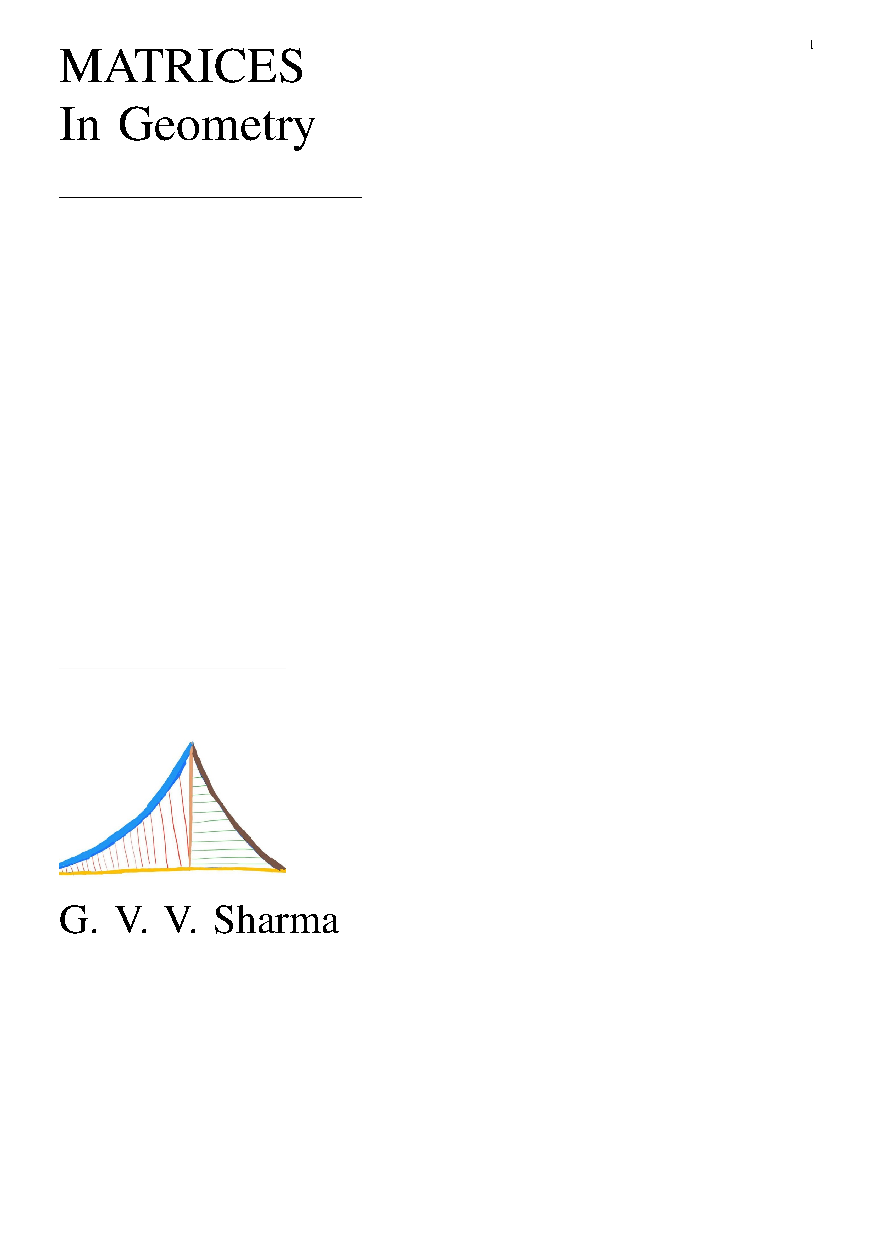
\includegraphics[width=0.75\columnwidth]{chapters/12/6/3/8/figs/main.png}
		\caption{}
		\label{fig:12/6/3/8}
  	\end{figure}
The equation of the conic can be represented as
\begin{align}
\vec{x}^{\top}\myvec{1&0\\0&0}\vec{x}+2\myvec{-2&\frac{-1}{2}}\vec{x}+4=0
\end{align}
So,
\begin{align}
\vec{V}=\myvec{1&0\\0&0},
\vec{u}^{\top}=\myvec{-2&\frac{-1}{2}},
f=4
\end{align}
The direction vector of the line passing through (2,0) and (4,4) is 
\begin{align}
\vec{m}=\myvec{1\\2}
\implies
\vec{n}=\myvec{2\\-1}.
\end{align}
The eigenvector corresponding to the zero eigenvalue is 
\begin{align}
\vec{p}_1=\myvec{0\\1},
\end{align}
In
\eqref{eq:conic_tangent_q_eigen},
\begin{align}
	\kappa=\frac{\myvec{0&1}\myvec{-2\\ \frac{-1}{2}}}{\myvec{0&1}\myvec{2\\-1}}
	=\frac{1}{2}
\end{align}
Substituting  $\kappa$,
from 
\eqref{eq:conic_tangent_q_eigen},
\begin{align}
	\myvec{\sbrak{\myvec{-2\\\frac{-1}{2}}+\frac{1}{2}\myvec{2\\-1}}^{\top} \\ \myvec{1&0\\0&0}}\vec{q} &= \myvec{-4 \\ \frac{1}{2}\myvec{2\\-1}-\myvec{-2\\\frac{-1}{2}}}\\
	\implies
	\myvec{-1&-1 \\ 1&0 \\ 0&0}\vec{q}&=\myvec{-4 \\ 3 \\ 0}
\end{align}
yielding
\begin{align}
\myvec{-1&-1 \\ 1&0}\vec{q} = \myvec{-4\\3}
\end{align}
The augmented matrix is 
\begin{align*}
  \myvec{
                -1&-1&\vrule&-4\\
	        1&0&\vrule&3}
  \xleftrightarrow[]{R_1 \leftarrow R_1+ 2R_2}
     \myvec{
	         1&-1&\vrule&2\\
	         1&0&\vrule&3}
      \\
 \xleftrightarrow[]{R_2 \leftarrow R_2 - R_1}
     \myvec{
	         1&-1&\vrule&2\\
	         0&1&\vrule&1}
 \xleftrightarrow[]{R_1 \leftarrow R_1 + R_2}
     \myvec{
	         1&0&\vrule&3\\
	         0&1&\vrule&1}
      \\ \implies \vec{q}=\myvec{3\\1}
\end{align*}
which is the desired 
point of contact.
See Fig. 
		\ref{fig:12/6/3/8}.



\iffalse
\latexprintindex
\fi

\end{document}


All codes for this section are available at
\begin{lstlisting}
	codes/triangle/sides.py
\end{lstlisting}
\end{enumerate}

\subsection{Formulae}
\begin{enumerate}[label=\thesection.\arabic*.,ref=\thesection.\theenumi]
\numberwithin{equation}{enumi}
\item The equation of a line is given by 
\begin{align}
			\label{eq:app-line-school}
	y &= mx + c
	\\
	\implies \myvec{x \\ y} &= \myvec{x \\ 
	 mx + c} =\myvec{0 \\ c} + x\myvec{1 \\ m}
\end{align}
			yielding \eqref{eq:geo-param}.
\item 			\eqref{eq:app-line-school} can also be expressed as
\begin{align}
	y - mx &= c 
	\\
	\implies \myvec{-m & 1}\myvec{x \\ y} &= c
\end{align}
			yielding \eqref{eq:geo-normal}.
		\item The direction vector is 
\begin{align}
			\label{eq:app-line-school-dir}
\vec{m} = \myvec{1 \\ m}
\end{align}
and the normal vector is
\begin{align}
\vec{n}=\myvec{-m \\ 1}
			\label{eq:app-line-school-normal}
\end{align}
  \item From \eqref{eq:geo-param}, 
	  if $\vec{A},\vec{D}$ and $\vec{C}$ are on the same line,
		\label{prop:app-lin-dep}
\begin{align}
			\vec{D}=\vec{A}+q\vec{m} 
			\\ 
			\vec{C}=\vec{D}+p\vec{m} \\
			\label{eq:app-collinear} 
			\implies 	p\brak{\vec{D}-\vec{A}} 
			+ q\brak{\vec{D}-\vec{C}} = 0, \quad p, q \ne 0 \\ 
			\implies \vec{D} = \frac{p\vec{A}+q\vec{C}}{p+q} 
			\end{align} 
			yielding \eqref{eq:section_formula} upon substituting \begin{align} k = \frac{p}{q}. \end{align} 
			$\brak{\vec{D}-\vec{A}}, \brak{\vec{D}-\vec{C}}$ 
		are then said to be {\em linearly dependent}.
	\item If $\vec{A}, \vec{B}, \vec{C}$ are collinear,  from \eqref{eq:geo-normal}, \begin{align}
	 \vec{n}^{\top}\vec{A} &=  c 
	 \\
	 \vec{n}^{\top}\vec{B} &=  c 
	 \\
	 \vec{n}^{\top}\vec{C} &=  c 
\end{align}
which can be expressed as 
\begin{align}
		\label{prop:app-lin-eq}
	\myvec{ \vec{A} & \vec{B} & \vec{C}}^{\top}\vec{n} = c\myvec{1 \\ 1 \\ 1}
	\\
	\equiv \myvec{ \vec{A} & \vec{B} & \vec{C}}^{\top}\vec{n} = \myvec{1 \\ 1 \\ 1}
		\label{prop:app-lin-eq-unit-mat},
	\\
	\implies 
	\myvec{ 1 & 1 &1 \\ \vec{A} & \vec{B} & \vec{C}}^{\top}\myvec{\vec{n} \\ -1} &= \vec{0}
		\label{prop:app-lin-dep-rank}
\end{align}
yielding
		\begin{align}
			\label{eq:app-line-rank-2}
			\rank{\myvec{1 & 1 & 1 \\ \vec{A}& \vec{B}&\vec{C}}} = 2
		\end{align}
			  Rank is defined to be the number of linearly indpendent rows or columns of a matrix.
		\item
The equation of a line can also be expressed as
\begin{align}
	 \vec{n}^{\top}\vec{x} &=   1
		\label{prop:app-lin-eq-unit}
\end{align}
	  \end{enumerate}

\subsection{Median}
\input{chapters/triangle/median}
\subsection{Altitude}
\input{chapters/triangle/altitude}
\subsection{Perpendicular Bisector}
\input{chapters/triangle/perp-bisect}
\subsection{Angle Bisector}
\input{chapters/triangle/angle-bisect}
\subsection{Eigenvalues and Eigenvectors}
\input{chapters/triangle/eigen}
\subsection{Formulae}
	\begin{figure}[H]
		\centering
 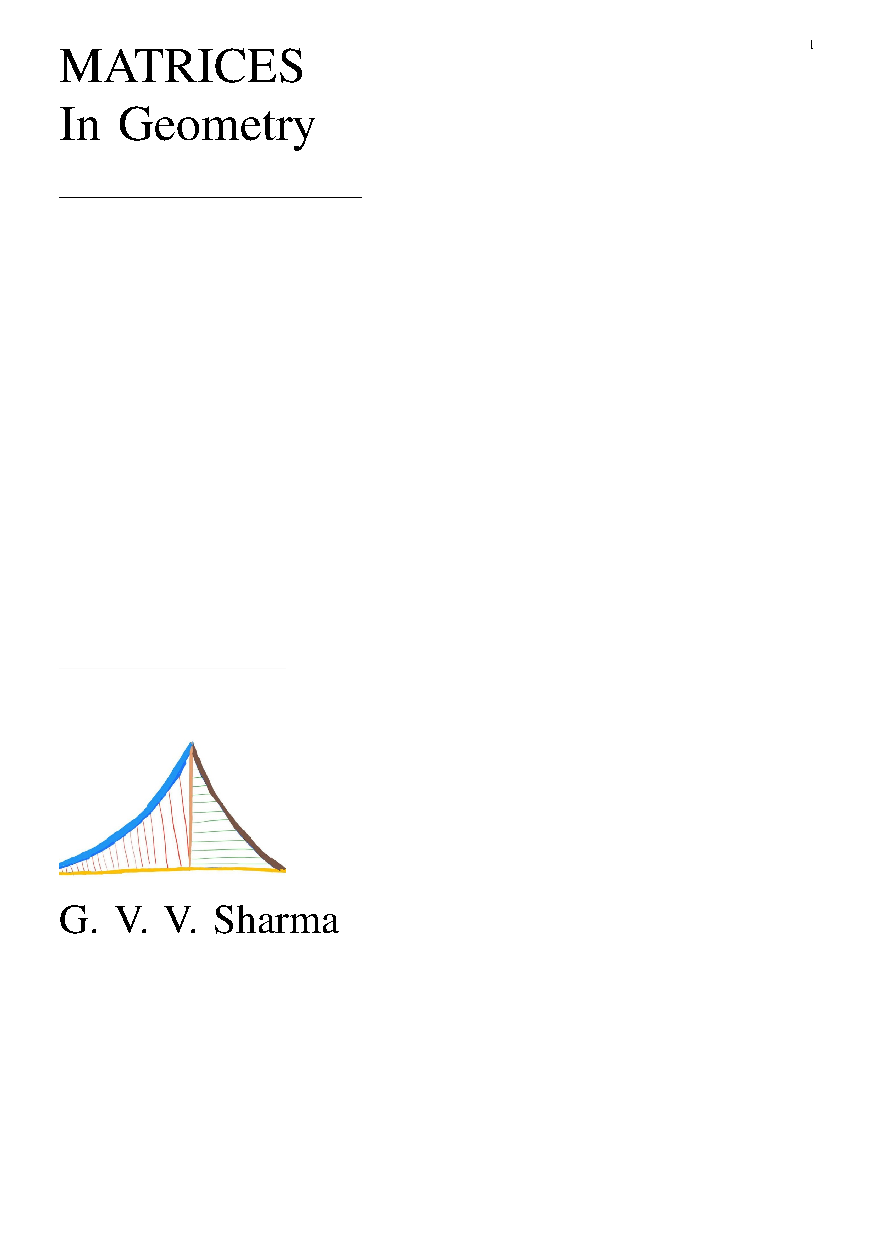
\includegraphics[width=0.75\columnwidth]{chapters/12/6/3/8/figs/main.png}
		\caption{}
		\label{fig:12/6/3/8}
  	\end{figure}
The equation of the conic can be represented as
\begin{align}
\vec{x}^{\top}\myvec{1&0\\0&0}\vec{x}+2\myvec{-2&\frac{-1}{2}}\vec{x}+4=0
\end{align}
So,
\begin{align}
\vec{V}=\myvec{1&0\\0&0},
\vec{u}^{\top}=\myvec{-2&\frac{-1}{2}},
f=4
\end{align}
The direction vector of the line passing through (2,0) and (4,4) is 
\begin{align}
\vec{m}=\myvec{1\\2}
\implies
\vec{n}=\myvec{2\\-1}.
\end{align}
The eigenvector corresponding to the zero eigenvalue is 
\begin{align}
\vec{p}_1=\myvec{0\\1},
\end{align}
In
\eqref{eq:conic_tangent_q_eigen},
\begin{align}
	\kappa=\frac{\myvec{0&1}\myvec{-2\\ \frac{-1}{2}}}{\myvec{0&1}\myvec{2\\-1}}
	=\frac{1}{2}
\end{align}
Substituting  $\kappa$,
from 
\eqref{eq:conic_tangent_q_eigen},
\begin{align}
	\myvec{\sbrak{\myvec{-2\\\frac{-1}{2}}+\frac{1}{2}\myvec{2\\-1}}^{\top} \\ \myvec{1&0\\0&0}}\vec{q} &= \myvec{-4 \\ \frac{1}{2}\myvec{2\\-1}-\myvec{-2\\\frac{-1}{2}}}\\
	\implies
	\myvec{-1&-1 \\ 1&0 \\ 0&0}\vec{q}&=\myvec{-4 \\ 3 \\ 0}
\end{align}
yielding
\begin{align}
\myvec{-1&-1 \\ 1&0}\vec{q} = \myvec{-4\\3}
\end{align}
The augmented matrix is 
\begin{align*}
  \myvec{
                -1&-1&\vrule&-4\\
	        1&0&\vrule&3}
  \xleftrightarrow[]{R_1 \leftarrow R_1+ 2R_2}
     \myvec{
	         1&-1&\vrule&2\\
	         1&0&\vrule&3}
      \\
 \xleftrightarrow[]{R_2 \leftarrow R_2 - R_1}
     \myvec{
	         1&-1&\vrule&2\\
	         0&1&\vrule&1}
 \xleftrightarrow[]{R_1 \leftarrow R_1 + R_2}
     \myvec{
	         1&0&\vrule&3\\
	         0&1&\vrule&1}
      \\ \implies \vec{q}=\myvec{3\\1}
\end{align*}
which is the desired 
point of contact.
See Fig. 
		\ref{fig:12/6/3/8}.

\subsection{Matrices}
The mid point of $PB$ is
\begin{align}
\vec{M} =\frac{1}{2}(\vec{P}+\vec{B})
	= \myvec{4 \\ -2}  
\end{align}
which is equal to the direction vector of $OM$.
\begin{align}
\because \vec{M} \equiv
	 \myvec{1 \\ -\frac{1}{2}},
	m = -\frac{1}{2}
\end{align}
which is the desired slope.
See 
		\figref{fig:11/10/1/5}.
	\begin{figure}[!ht]
		\centering
 \includegraphics[width=\columnwidth]{chapters/11/10/1/5/figs/line.png}
		\caption{}
		\label{fig:11/10/1/5}
  	\end{figure}

\newpage
\section{Vectors}
\subsection{Addition and Subtraction}
\begin{enumerate}[label=\thesubsection.\arabic*,ref=\thesubsection.\theenumi]
\item Find the sum of the vectors $\vec{a}=\hat{i}-2\hat{j}+\hat{k}$, $\vec{b}=-2\hat{i}+4\hat{j}+5\hat{k}$ and $\vec{c}=\hat{i}-6\hat{j}-7\hat{k}$.
\item 

	In triangle ABC 
		(\figref{fig:chapters/12/10/2/18/}),
		which of the following is not true:
 \begin{enumerate}
         \item $\overrightarrow{AB}+\overrightarrow{BC}+\overrightarrow{CA}$=$\vec{0}$
         \item $\overrightarrow{AB}+\overrightarrow{BC}-\overrightarrow{CA}$=$\vec{0}$
         \item $\overrightarrow{AB}+\overrightarrow{BC}-\overrightarrow{CA}$=$\vec{0}$
         \item $\overrightarrow{AB}-\overrightarrow{BC}+\overrightarrow{CA}$=$\vec{0}$
\end{enumerate}
\begin{figure}[!ht]
\centering
\includegraphics[width = \columnwidth]{./chapters/12/10/2/18/figs/triangle.png}
\caption{}
	\label{fig:chapters/12/10/2/18/}
\end{figure}
\solution
		\begin{align}
	\overrightarrow{AB}+\overrightarrow{BC}+\overrightarrow{CA} &=
\vec{B}-\vec{A} + \vec{C} - \vec{B} + \vec{A} - \vec{C}
= 0
\\
	\overrightarrow{AB}+\overrightarrow{BC}-\overrightarrow{AC} &=
\vec{B}-\vec{A} + \vec{C} - \vec{B} - (\vec{C} - \vec{A})
= 0
\\
	\overrightarrow{AB}+\overrightarrow{BC}+\overrightarrow{AC} &=
\vec{B}-\vec{A} + \vec{C} - \vec{B} + \vec{C} - \vec{A}
= 2(\vec{C}-\vec{A})
\\
	\overrightarrow{AB}-\overrightarrow{CB}+\overrightarrow{CA} &=
\vec{B}-\vec{A} - (\vec{B} - \vec{C}) + \vec{A} - \vec{C}
= 0
\end{align}

\item A girl walks 4 km towards west, then she walks 3 km in a direction 30$^{\circ}$ east of north and stops. Determine the girl's displacement from her initial point of departure.\\
	\solution
		See  
\figref{fig:chapters/12/10/5/3Fig1}.
Let the initial position
be
\begin{align}
	\vec{A}=\myvec{0\\0}
\end{align}
After going west, the position becomes
\begin{align}
			\vec{B}=\myvec{-4\\0}
\end{align}
If the final position be $\vec{C}$, from the given information,
\begin{align}
	 \vec{C}-\vec{B}=3\myvec{\cos{60\degree}\\\sin{60\degree}}
	 \implies 
	\vec{C}  
=\myvec{-\frac{5}{2}\\[2pt] \frac{3\sqrt{3}}{2}}
\end{align}
which is the desired displacement. 
\begin{figure}[H] 
 \begin{center} 
 \includegraphics[width=0.75\columnwidth]{chapters/12/10/5/3/figs/fig.pdf} 
 \end{center} 
\caption{} 
\label{fig:chapters/12/10/5/3Fig1} 
\end{figure}

\item Without using distance formula, show that points A(– 2, – 1), B(4, 0), C(3, 3) and D(–3, 2) are the vertices of a parallelogram.
\label{chapters/11/10/1/9}
\\
\solution
	  From \eqref{eq:two-pgm},
\begin{align}
\vec{A}-\vec{B} = 
\vec{D}-\vec{C} =  \myvec{-6\\-1}
\end{align}
Hence, $ABCD$ is a parallelogram.
See \figref{fig:chapters/11/10/1/91}.
\begin{figure}[H]
  \centering
   %\includegraphics[width=0.75\columnwidth]{chapters/11/10/1/9/figs/paralellogram.png}
   \includegraphics[width=0.75\columnwidth]{chapters/11/10/1/9/figs/fig.pdf}
    \caption{}
     \label{fig:chapters/11/10/1/91}  
\end{figure}




\item The fourth vertex $\vec{D}$ of a parallelogram $\vec{ABCD}$ whose three vertices are
	$\vec{A} (–2, 3), \vec{B} (6, 7)\text { and } \vec{C} (8, 3)$ is
\begin{enumerate}
	\item $(0, 1)$
	\item $(0, –1)$
	\item $ (–1,0)$
	\item$(1, 0)$
\end{enumerate}
\item Points $\vec{A}(4,3), \vec{B}(6,4),\vec{C}(5,-6)$  and  $\vec{D}(-3,5)$ are the vertices of a parallelogram.
\end{enumerate}

\subsection{Section Formula}
See  
\figref{fig:chapters/10/7/4/6Fig1}.
\begin{figure}[H]
 \begin{center}
 \includegraphics[width=0.75\columnwidth]{chapters/10/7/4/6/figs/fig.pdf}
 \end{center}
\caption{}
\label{fig:chapters/10/7/4/6Fig1}
\end{figure}
	Using section formula
	  \eqref{eq:section_formula},
\begin{align}
\vec{D} =\frac{3\vec{A}+\vec{B}}{4}
	=\frac{1}{4}\myvec{13\\ 23}
	\\
\vec{E} =\frac{3\vec{A}+\vec{C}}{4}
	=\frac{1}{4}\myvec{19\\ 20}
	\\
	\vec{A}- \vec{D} 
	=\frac{1}{4}\myvec{3\\ 1},\,
	  \vec{A}- \vec{E}  
	=\frac{1}{4}\myvec{-3\\ 1}
	\\
	\vec{A}- \vec{B} =\myvec{3\\1},
	  \vec{B}-\vec{C} =\myvec{-6\\3}
\end{align}
yielding
\begin{align}
ar(ABD) =\frac{1}{2} \norm{\brak{\vec{A}-\vec{D}}  \times 
   \brak{\vec{A}- \vec{E}}} 
	=	\frac{15}{32}
	\\
	  ar(ABC) =\frac{1}{2} \norm{\brak{\vec{A}-\vec{B}}  \times 
   \brak{\vec{B}- \vec{C}}} 
	=	\frac{15}{2}
	\\
	\implies \frac{ar\brak{ADE}}{ar\brak{ABC}}=\frac{1}{16}
\end{align}

\subsection{Rank}
\begin{enumerate}[label=\thesubsection.\arabic*,ref=\thesubsection.\theenumi]
\item Determine if the points $(1,5),(2,3)$ and $(-2,-11)$ are collinear.
	\\
	\solution
Use		\eqref{prop:lin-dep-rank}.
%		\begin{enumerate}[label=\thesubsection.\arabic*, ref=\thesubsection.\theenumi]
    \item The value of $m$ which makes the points $(0,0)$, $(2m, -4)$, and $(3,6)$ collinear, is \underline{\hspace{1cm}}.
    \hfill (10, 2022)
		\item If $\vec{A}(1, 2)$, $\vec{O}(0, 0)$, and $\vec{C}(a, 6)$ are collinear, then the value of $a$ is
		\hfill (10, 2021)
	\item Show that the points $A(-2\hat{i} + 3\hat{j} + 5\hat{k})$, $B(\hat{i} + 2\hat{j} + 3\hat{k})$, and $C(7\hat{i} - \hat{k})$ are collinear. \hfill (12, 2019)
	\item Using vectors, prove that the points $(2, -1, 3)$, $(3, -5, 1)$, and $(-1, 11, 9)$ are collinear. \hfill (12, 2019)
\item Find the value of $p$ for which the points $(-5, 1)$, $(1, p)$, and $(4, -2)$ are collinear. \hfill (10, 2019)
\item Find a relation between $x$ and $y$ if the points $A(x, y)$, $B(-4, 6)$, and $C(-2, 3)$ are collinear. \hfill (10, 2019)
\item For what value of $p$ are the points $(2, 1)$, $(p, -1)$, and $(-1, 3)$ collinear? \hfill (10, 2019)
\end{enumerate}

\item Show that the points $\vec{A}(1,2,7), \vec{B}(2,6,3)$ and $\vec{C}(3,10,-1)$ are collinear.
	\\
	\solution
%		\begin{enumerate}[label=\thesubsection.\arabic*, ref=\thesubsection.\theenumi]
    \item The value of $m$ which makes the points $(0,0)$, $(2m, -4)$, and $(3,6)$ collinear, is \underline{\hspace{1cm}}.
    \hfill (10, 2022)
		\item If $\vec{A}(1, 2)$, $\vec{O}(0, 0)$, and $\vec{C}(a, 6)$ are collinear, then the value of $a$ is
		\hfill (10, 2021)
	\item Show that the points $A(-2\hat{i} + 3\hat{j} + 5\hat{k})$, $B(\hat{i} + 2\hat{j} + 3\hat{k})$, and $C(7\hat{i} - \hat{k})$ are collinear. \hfill (12, 2019)
	\item Using vectors, prove that the points $(2, -1, 3)$, $(3, -5, 1)$, and $(-1, 11, 9)$ are collinear. \hfill (12, 2019)
\item Find the value of $p$ for which the points $(-5, 1)$, $(1, p)$, and $(4, -2)$ are collinear. \hfill (10, 2019)
\item Find a relation between $x$ and $y$ if the points $A(x, y)$, $B(-4, 6)$, and $C(-2, 3)$ are collinear. \hfill (10, 2019)
\item For what value of $p$ are the points $(2, 1)$, $(p, -1)$, and $(-1, 3)$ collinear? \hfill (10, 2019)
\end{enumerate}

\item Show that the vectors $2\hat{i}-3\hat{j}+4\hat{k}$ and $-4\hat{i}+6\hat{j}-8\hat{k}$ are collinear.
   \\ 
    \solution 
%		\begin{enumerate}[label=\thesubsection.\arabic*, ref=\thesubsection.\theenumi]
    \item The value of $m$ which makes the points $(0,0)$, $(2m, -4)$, and $(3,6)$ collinear, is \underline{\hspace{1cm}}.
    \hfill (10, 2022)
		\item If $\vec{A}(1, 2)$, $\vec{O}(0, 0)$, and $\vec{C}(a, 6)$ are collinear, then the value of $a$ is
		\hfill (10, 2021)
	\item Show that the points $A(-2\hat{i} + 3\hat{j} + 5\hat{k})$, $B(\hat{i} + 2\hat{j} + 3\hat{k})$, and $C(7\hat{i} - \hat{k})$ are collinear. \hfill (12, 2019)
	\item Using vectors, prove that the points $(2, -1, 3)$, $(3, -5, 1)$, and $(-1, 11, 9)$ are collinear. \hfill (12, 2019)
\item Find the value of $p$ for which the points $(-5, 1)$, $(1, p)$, and $(4, -2)$ are collinear. \hfill (10, 2019)
\item Find a relation between $x$ and $y$ if the points $A(x, y)$, $B(-4, 6)$, and $C(-2, 3)$ are collinear. \hfill (10, 2019)
\item For what value of $p$ are the points $(2, 1)$, $(p, -1)$, and $(-1, 3)$ collinear? \hfill (10, 2019)
\end{enumerate}

\item Show that the points (2, 3, 4), (–1, –2, 1), (5, 8, 7) are collinear.
		\\
		\solution
	%	\begin{enumerate}[label=\thesubsection.\arabic*, ref=\thesubsection.\theenumi]
    \item The value of $m$ which makes the points $(0,0)$, $(2m, -4)$, and $(3,6)$ collinear, is \underline{\hspace{1cm}}.
    \hfill (10, 2022)
		\item If $\vec{A}(1, 2)$, $\vec{O}(0, 0)$, and $\vec{C}(a, 6)$ are collinear, then the value of $a$ is
		\hfill (10, 2021)
	\item Show that the points $A(-2\hat{i} + 3\hat{j} + 5\hat{k})$, $B(\hat{i} + 2\hat{j} + 3\hat{k})$, and $C(7\hat{i} - \hat{k})$ are collinear. \hfill (12, 2019)
	\item Using vectors, prove that the points $(2, -1, 3)$, $(3, -5, 1)$, and $(-1, 11, 9)$ are collinear. \hfill (12, 2019)
\item Find the value of $p$ for which the points $(-5, 1)$, $(1, p)$, and $(4, -2)$ are collinear. \hfill (10, 2019)
\item Find a relation between $x$ and $y$ if the points $A(x, y)$, $B(-4, 6)$, and $C(-2, 3)$ are collinear. \hfill (10, 2019)
\item For what value of $p$ are the points $(2, 1)$, $(p, -1)$, and $(-1, 3)$ collinear? \hfill (10, 2019)
\end{enumerate}

\item In each of the following, find the value of '$k$', for which the points are collinear.
\begin{enumerate}
\item $(7, –2), (5, 1), (3, k)$
\item $(8, 1), (k, – 4), (2, –5)$
\end{enumerate}
		\label{10/7/3/2}
\solution
	%	\begin{enumerate}[label=\thesubsection.\arabic*, ref=\thesubsection.\theenumi]
    \item The value of $m$ which makes the points $(0,0)$, $(2m, -4)$, and $(3,6)$ collinear, is \underline{\hspace{1cm}}.
    \hfill (10, 2022)
		\item If $\vec{A}(1, 2)$, $\vec{O}(0, 0)$, and $\vec{C}(a, 6)$ are collinear, then the value of $a$ is
		\hfill (10, 2021)
	\item Show that the points $A(-2\hat{i} + 3\hat{j} + 5\hat{k})$, $B(\hat{i} + 2\hat{j} + 3\hat{k})$, and $C(7\hat{i} - \hat{k})$ are collinear. \hfill (12, 2019)
	\item Using vectors, prove that the points $(2, -1, 3)$, $(3, -5, 1)$, and $(-1, 11, 9)$ are collinear. \hfill (12, 2019)
\item Find the value of $p$ for which the points $(-5, 1)$, $(1, p)$, and $(4, -2)$ are collinear. \hfill (10, 2019)
\item Find a relation between $x$ and $y$ if the points $A(x, y)$, $B(-4, 6)$, and $C(-2, 3)$ are collinear. \hfill (10, 2019)
\item For what value of $p$ are the points $(2, 1)$, $(p, -1)$, and $(-1, 3)$ collinear? \hfill (10, 2019)
\end{enumerate}

\item Find a relation between $x$ and $y$ if the points $(x, y), (1, 2)$  and  $(7, 0)$ are collinear.
\\
\solution
	%\begin{enumerate}[label=\thesubsection.\arabic*, ref=\thesubsection.\theenumi]
    \item The value of $m$ which makes the points $(0,0)$, $(2m, -4)$, and $(3,6)$ collinear, is \underline{\hspace{1cm}}.
    \hfill (10, 2022)
		\item If $\vec{A}(1, 2)$, $\vec{O}(0, 0)$, and $\vec{C}(a, 6)$ are collinear, then the value of $a$ is
		\hfill (10, 2021)
	\item Show that the points $A(-2\hat{i} + 3\hat{j} + 5\hat{k})$, $B(\hat{i} + 2\hat{j} + 3\hat{k})$, and $C(7\hat{i} - \hat{k})$ are collinear. \hfill (12, 2019)
	\item Using vectors, prove that the points $(2, -1, 3)$, $(3, -5, 1)$, and $(-1, 11, 9)$ are collinear. \hfill (12, 2019)
\item Find the value of $p$ for which the points $(-5, 1)$, $(1, p)$, and $(4, -2)$ are collinear. \hfill (10, 2019)
\item Find a relation between $x$ and $y$ if the points $A(x, y)$, $B(-4, 6)$, and $C(-2, 3)$ are collinear. \hfill (10, 2019)
\item For what value of $p$ are the points $(2, 1)$, $(p, -1)$, and $(-1, 3)$ collinear? \hfill (10, 2019)
\end{enumerate}

\item If three points $(x, -1), (2, 1)$ and $(4, 5)$ are collinear, find the value of $x$.
\label{chapters/11/10/1/8}
%The mid point of $PB$ is
\begin{align}
\vec{M} =\frac{1}{2}(\vec{P}+\vec{B})
	= \myvec{4 \\ -2}  
\end{align}
which is equal to the direction vector of $OM$.
\begin{align}
\because \vec{M} \equiv
	 \myvec{1 \\ -\frac{1}{2}},
	m = -\frac{1}{2}
\end{align}
which is the desired slope.
See 
		\figref{fig:11/10/1/5}.
	\begin{figure}[!ht]
		\centering
 \includegraphics[width=\columnwidth]{chapters/11/10/1/5/figs/line.png}
		\caption{}
		\label{fig:11/10/1/5}
  	\end{figure}

\item If three points $(h, 0), (a, b)$ and $(0, k)$ lie on a line, 
show that 
\begin{align}
\frac{a}{h}+\frac{b}{k}=1
\end{align}
\label{chapters/11/10/1/13}
%The mid point of $PB$ is
\begin{align}
\vec{M} =\frac{1}{2}(\vec{P}+\vec{B})
	= \myvec{4 \\ -2}  
\end{align}
which is equal to the direction vector of $OM$.
\begin{align}
\because \vec{M} \equiv
	 \myvec{1 \\ -\frac{1}{2}},
	m = -\frac{1}{2}
\end{align}
which is the desired slope.
See 
		\figref{fig:11/10/1/5}.
	\begin{figure}[!ht]
		\centering
 \includegraphics[width=\columnwidth]{chapters/11/10/1/5/figs/line.png}
		\caption{}
		\label{fig:11/10/1/5}
  	\end{figure}

\item Show that the points A (1, -2, -8), B (5, 0, -2) and C (11, 3, 7) are collinear, and find the ratio in which B divides AC.\\
\item lf the points $\vec{A}(1,2),\vec{0}(0,0)\text{ and }\vec{C}(a,b)$ are collinear,then
\begin{enumerate}
\item a=b
\item a=2b
\item 2a=b
\item a=-b
\end{enumerate}
\end{enumerate}
True/false
\begin{enumerate}[label=\thesection.\arabic*,ref=\thesection.\theenumi,resume*]
	\item $\triangle\vec{A}\vec{B}\vec{C}$ with vertices $\vec{A}(-2,0), \vec{B}(2,0) \text{ and }\vec{C}(0,2)$ is similar to $\triangle \vec{DEF}$  with vertices $\vec {D}(-4,0),\vec{E}(4,0)  \text{ and } \vec{F}(0,4)$  
	\item Point $ (-4,2)$ lies on the line segment joining the points $ \vec{A}(-4,6) \text{ and } \vec{B}(-4,-6)$
 \item The points $(0,5),(0,-9)\text{ and }(3,6)$ are collinear
\item Points $\vec{A}(3,1), \vec{B}(12,-2) \text{ and } \vec {C}(0,2)$ cannot be the vertices of a triangle
\item Find the value of $m$ if the points $(5,1),(-2,-3) \text{ and }(8,2m)$ are collinear.
\item Find the values of k if the points $\vec{A}(k+1,2k),\vec{B}(3k,2k+3)\text{ and }\vec{C}(5k-1,5k)$ are collinear
\item Using vectors, find the value of $k$ such that the points $(k,-10,3)$, $(1,-1,3)$ $\text{ and }$ $(3,5,3)$ are collinear.
\end{enumerate}

\subsection{Length}
\begin{enumerate}[label=\thesection.\arabic*,ref=\thesection.\theenumi]
\item Compute the magnitude of the following vectors:
\begin{align}
	\vec{a}&=\hat{i}+\hat{j}+\hat{k}
	\\
	\vec{b}&=2\hat{i}-7\hat{j}-3\hat{k}
	\\
	\vec{c}&=\frac{1}{\sqrt{3}}\hat{i}+\frac{1}{\sqrt{3}}\hat{j}-\frac{1}{3}\hat{k}
\end{align}
    \solution 
		Let 
\begin{align}
	\vec{a} = \myvec{1\\1\\1} , \vec{b} = \myvec{2\\ -7 \\ 3}, 
\vec{c} = \myvec{\dfrac{1}{\sqrt{3}}\\[2ex] \dfrac{1}{\sqrt{3}} \\[2ex] -\dfrac{1}{\sqrt{3}}} 
\label{eq:chapters/12/10/2/1/1}
\end{align}
Then
\begin{align}
	{\vec{a}^{\top}\vec{a}} &= \myvec{1  &  1  &  1}\myvec{1\\1\\1} = 3
\\
\implies 
	\norm{\vec{a}}&=\sqrt{3}, 
	\label{eq:chapters/12/10/2/1/3}
\end{align}
		from \eqref{eq:side-length}. Similarly,
\begin{align}
	\norm{\vec{b}}&=\sqrt{\vec{b}^{\top}\vec{b}}= \sqrt{62}, 
	\label{eq:chapters/12/10/2/1/4}
	\\ \norm{\vec{c}}&=\sqrt{\vec{c}^{\top}\vec{c}}	
=1
	\label{eq:chapters/12/10/2/1/5}
\end{align}




\item Find the value of x for which $x(\hat{i}+\hat{j}+\hat{k})$ is a unit vector.\\
	\solution
		\begin{align} 
\because
\vec{x}=x\myvec{1\\1\\1},
\norm{\vec{x}}=1
\implies 
x\sqrt{3}=1
\\
	\text{or, }x=\frac{1}{\sqrt{3}}
\end{align}   

\item If $\vec{a}=\vec{b}+\vec{c}$, then is it true that $|\vec{a}|=|\vec{b}|+|\vec{c}|$? Justify your answer.\\
	\solution
		Let 
\begin{align}
	\vec{a} = \myvec{1\\1\\1} , \vec{b} = \myvec{2\\ -7 \\ 3}, 
\vec{c} = \myvec{\dfrac{1}{\sqrt{3}}\\[2ex] \dfrac{1}{\sqrt{3}} \\[2ex] -\dfrac{1}{\sqrt{3}}} 
\label{eq:chapters/12/10/2/1/1}
\end{align}
Then
\begin{align}
	{\vec{a}^{\top}\vec{a}} &= \myvec{1  &  1  &  1}\myvec{1\\1\\1} = 3
\\
\implies 
	\norm{\vec{a}}&=\sqrt{3}, 
	\label{eq:chapters/12/10/2/1/3}
\end{align}
		from \eqref{eq:side-length}. Similarly,
\begin{align}
	\norm{\vec{b}}&=\sqrt{\vec{b}^{\top}\vec{b}}= \sqrt{62}, 
	\label{eq:chapters/12/10/2/1/4}
	\\ \norm{\vec{c}}&=\sqrt{\vec{c}^{\top}\vec{c}}	
=1
	\label{eq:chapters/12/10/2/1/5}
\end{align}




\item If $\overrightarrow {a}$ is a nonzero vector of magnitude `a' and $\lambda$ a nonzero scalar, then $\lambda\overrightarrow {a}$ is a unit vector if
\begin{enumerate} 
\item $\lambda=1$ 
\item $\lambda=-1$
\item $a=\abs{\lambda}$
\item $a=1/\abs{\lambda}$  
\end{enumerate}

\end{enumerate}

%
\subsection{Direction}
\begin{enumerate}[label=\thesection.\arabic*,ref=\thesection.\theenumi]
\item For given vectors, $\vec{a}=2\hat{i}-\hat{j}+2\hat{k}$ and $\vec{b}=-\hat{i}+\hat{j}-\hat{k}$ , find the unit vector in the
direction of the vector $\vec{a}+\vec{b}$.
        \label{prob:12/10/2/9}
\\
    \solution 
		\begin{align}
	\because \vec a + \vec b = \myvec{ 2\\-1\\2 } + \myvec{ -1\\1\\-1 },
= \myvec{ 1\\0\\1 },
\\
	\norm{\vec a + \vec b } = \sqrt{2}
	\\
	\implies \frac{\vec a + \vec b }{\norm{\vec a + \vec b }} = \frac{1}{\sqrt{2}}\myvec{ 1\\0\\1 }
\end{align}
which, from  \eqref{eq:unit-vec} is the desired the unit vector.
		





\item Find a vector in the direction of vector $5\hat{i}-\hat{j}+2\hat{k}$ which has magnitude 8 units.
        \label{prob:12/10/2/10const}
   \\ 
    \solution 
		Let the required vector be 
    \begin{align}
c\myvec{5\\-1\\2}.
    \end{align}
    From the given information, 
    \begin{align}
        \norm{c\myvec{5\\-1\\2\\}} =  8 \\
	    \implies \abs{c} = \frac{4\sqrt{30}}{15}
        \label{eq:12/10/2/10const}
    \end{align}


\item Find the unit vector in the direction of the vector $\vec{a}=\hat{i}+\hat{j}+2\hat{k}$.
\item Find the unit vector in the direction of vector $\overrightarrow{PQ}$ , where $\vec{P}$ and $\vec{Q}$ are the points
(1, 2, 3) and (4, 5, 6), respectively.
	\item 
Find a vector of magnitude 5 units, and parallel to the resultant of the vectors $\vec{a} = 2\hat{i}+3\hat{j}-\hat{k}$ and $\vec{b} = \hat{i}-2\hat{j}+\hat{k}$.
\\
\solution
		\begin{align}
\because     \Vec{a}=\myvec{
        2\\3\\-1
    },\Vec{b}=\myvec{
        1\\-2\\1
    }\\
	\vec{a}+\vec{b}=\myvec{
        3\\1\\0
    }
    \implies
	\norm{\vec{a}+\vec{b}}=\sqrt{10}
\end{align}
From problem
        \ref{prob:12/10/2/9},
the unit vector in the direction of 
${\vec{a}+\vec{b}}$
is
\begin{align}
	\frac{{\vec{a}+\vec{b}}}{\norm{\vec{a}+\vec{b}}}
=\frac{1}{\sqrt{10}}\myvec{
        3\\1\\0
    }
\end{align}
The desired vector can then be expressed as
\begin{align}
\pm\frac{5}{\sqrt{10}}\myvec{
        3\\1\\0
    }
\end{align}


\item Find the direction cosines of the vector joining the points $\vec{A}$ (1, 2, –3) and
$\vec{B}$(–1, –2, 1), directed from $\vec{A}$ to $\vec{B}$.
	\\
    \solution 
		The unit vector  in the direction of AB is 
\begin{align}
	\frac{\vec{B}-\vec{A}}{\norm{\vec{B}-\vec{A}}}
	= \frac{1}{3}{\myvec{-1\\-2\\2}}
\end{align}
and the direction cosines are the elements of the above vector.

\item Show that the vector $\hat{i}+\hat{j}+\hat{k}$ is equally inclined to the axes OX, OY and OZ.
	\\
\solution
		Since all entries of the given vector 
\begin{align}
\myvec{1\\1\\1}
\end{align}
are equal, it is equally inclined to the axes.

\item If a line has the direction ratios –18, 12, –4, then what are its direction cosines?
		\\
		\solution
		Let
\begin{align}
	\vec{A} =\myvec{-18\\12\\-4}
\end{align}
Then the unit direction vector of the line is
\begin{align}
		\frac{\vec{A}}{\norm{\vec{A}}} =
\myvec{\frac{-9}{11}\\[2pt] \frac{6}{11}\\[2pt] \frac{-2}{11}}
\end{align}

	\item Find the direction cosines of the sides of a triangle whose vertices are $\myvec{3\\ 5\\-4 }$, $\myvec{ -1\\1 \\2 }$ and $\myvec{-5 \\-5 \\-2 }$.
		\\
		\solution
		Let the vertices be
\begin{align}
\vec{A} = \myvec{3\\5\\-4},
\vec{B} = \myvec{-1\\1\\2},
\vec{C} = \myvec{-5\\-5\\-2}
\end{align}
%
The direction vectors of the sides are,
\begin{align}
\vec{A} - \vec{B} = \myvec{4\\4\\-6} = \vec{m_1},
\vec{B} - \vec{C} = \myvec{4\\6\\4} = \vec{m_2}, 
\\
\vec{C} - \vec{A} = \myvec{-8\\-10\\2} =\vec{m_3},
\end{align}
%
The corresponding unit vectors are then obtained as
\begin{align}
 \myvec{ \frac{2}{\sqrt{17}} \\[1pt] \frac{2}{\sqrt{17}} \\[1pt] \frac{-3}{\sqrt{17}} },
 \myvec{ \frac{2}{\sqrt{17}} \\[1pt] \frac{3}{\sqrt{17}} \\[1pt] \frac{2}{\sqrt{17}} }, 
 \myvec{ \frac{-4}{\sqrt{42}} \\[1pt] \frac{-5}{\sqrt{42}} \\[1pt] \frac{1}{\sqrt{42}} } 
\end{align}

\item Find the direction cosines of the vector $\hat{i}+2\hat{j}+3\hat{k}$.
	\\
    \solution 
		The unit vector in the direction of the given vector is 
\begin{align}
	\vec{A} =\frac{1}{\sqrt{14}}\myvec{1\\2\\3}
\end{align}

    \item Find the direction cosines of a line which makes equal angles with the coordinate
    axes.
		\\
		\solution
		Let $\alpha$ be the angle made by the line with the axes.  The unit direction vector can be expressed as
    \begin{align}
	    \vec{x} &= \myvec{\cos\alpha\\\cos\alpha\\\cos\alpha} 
	\implies
	    \norm{\vec{x}}  = 1
	\\
	    \text{or, }\cos\alpha &= \frac{1}{\sqrt{3}}
    \end{align}
    Thus the unit direction vector  of the given line is 
    \begin{align}
	    \vec{x} = \frac{1}{\sqrt{3}} \myvec{1 \\ 1 \\ 1} 
\end{align}
    

\item Write down a unit vector in XY-plane, making an angle of 30$^{\circ}$ with the positive direction of x-axis.\\
\end{enumerate}

\subsection{Scalar Product}
\begin{enumerate}[label=\thesubsection.\arabic*, ref=\thesubsection.\theenumi]
\item The angle between the vectors $\hat{i} - \hat{j}$ and $\hat{j} - \hat{k}$ is \rule{1cm}{0.2pt}.
\hfill (12, 2020)
\item Find the angle between unit vectors $\overrightarrow{a}$ and $\overrightarrow{b}$ so that $\sqrt{3}\overrightarrow{a}$ - $\overrightarrow{b}$ is also a unit vector.
\hfill (12, 2020)
    \item If $\overrightarrow{a}, \overrightarrow{b}, \overrightarrow{c}$ are three non-zero unequal vectors such that $\overrightarrow{a} \cdot \overrightarrow{b} = \overrightarrow{a} \cdot \overrightarrow{c}$, then find the angle between $\overrightarrow{a}$ and $\overrightarrow{b} - \overrightarrow{c}$.
    \hfill (12, 2023)
    \item $\overrightarrow{a}$ and $\overrightarrow{b}$ are two unit vectors such that
    \begin{align}
        \left| 2\overrightarrow{a} + 3\overrightarrow{b} \right| = \left| 3\overrightarrow{a} - 2\overrightarrow{b} \right|.
    \end{align}
  Find the angle between $\overrightarrow{a}$ and $\overrightarrow{b}$.
    \hfill (12, 2023)
	\item Find the angle between the line $\overrightarrow{r} = \hat{i} - \hat{j} + \hat{k} + \lambda (3\hat{i} - \hat{j} + 2\hat{k})$ and the plane $\overrightarrow{r} \cdot (\hat{i} + \hat{j} + \hat{k}) = 3$.

		\hfill (12, 2019)
\item Find the magnitude of each of the vectors $\overrightarrow{\vec{a}}$ and $\overrightarrow{\vec{b}}$, having the same magnitude such that the angle between them is $60\degree$ and their scalar product is $\frac{9}{2}$. \hfill (12, 2018)
\item Find the acute angle between the planes $\vec{r}\cdot\brak{ \hat{i}-\hat{2j}-\hat{2k}}=1$ and $\vec{r}\cdot \brak{\hat{3i}-\hat{6j}+\hat{2k}}=0$

\hfill (12, 2018)
\item If $\hat{i}+\hat{j}+{k} ,  2\hat{i}+5\hat{j} ,  3\hat{i}+2\hat{j}-3{k} ,  \hat{i}-6\hat{j}-{k}$ respectively are the position vectors of points A, B, C and D, then find the angle between the straight lines AB and CD. Find whether $\overrightarrow{AB}$ and $\overrightarrow{CD}$ are collinear or not. 
\hfill (12, 2018) 
\item If vectors $\overrightarrow{a}$ and $\overrightarrow{b}$ are such that
      $\abs{\overrightarrow{a}} = \frac{1}{2}$, $\abs{\overrightarrow{b}} = \frac{4}{\sqrt{3}}$
      and $\abs{\overrightarrow{a} \times \overrightarrow{b}} = \frac{1}{\sqrt{3}}$, then find
      $\abs{\overrightarrow{a}\cdot \overrightarrow{b} }$. \hfill (12, 2016)
\item If $\overrightarrow{a}$ and $\overrightarrow{b}$ are unit vectors, then what is the angle between
      $\overrightarrow{a}$ and $\overrightarrow{b}$ for $\overrightarrow{a} - \sqrt{2}\overrightarrow{b}$ to be a unit vector? \hfill (12, 2016)
\item Find the acute angle between the planes
      $  \overrightarrow{r} \cdot \brak{\hat{i}-2\hat{j}-2\hat{k}} = 1$
      and
      $  \overrightarrow{r} \cdot \brak{3\hat{i}-6\hat{j}+2\hat{k}} = 0$.
    \hfill (12, 2019)                                                    


\end{enumerate}

\subsection{Formulae}
\begin{enumerate}[label=\thesubsection.\arabic*, ref=\thesubsection.\theenumi]
\item The angle between the vectors $\hat{i} - \hat{j}$ and $\hat{j} - \hat{k}$ is \rule{1cm}{0.2pt}.
\hfill (12, 2020)
\item Find the angle between unit vectors $\overrightarrow{a}$ and $\overrightarrow{b}$ so that $\sqrt{3}\overrightarrow{a}$ - $\overrightarrow{b}$ is also a unit vector.
\hfill (12, 2020)
    \item If $\overrightarrow{a}, \overrightarrow{b}, \overrightarrow{c}$ are three non-zero unequal vectors such that $\overrightarrow{a} \cdot \overrightarrow{b} = \overrightarrow{a} \cdot \overrightarrow{c}$, then find the angle between $\overrightarrow{a}$ and $\overrightarrow{b} - \overrightarrow{c}$.
    \hfill (12, 2023)
    \item $\overrightarrow{a}$ and $\overrightarrow{b}$ are two unit vectors such that
    \begin{align}
        \left| 2\overrightarrow{a} + 3\overrightarrow{b} \right| = \left| 3\overrightarrow{a} - 2\overrightarrow{b} \right|.
    \end{align}
  Find the angle between $\overrightarrow{a}$ and $\overrightarrow{b}$.
    \hfill (12, 2023)
	\item Find the angle between the line $\overrightarrow{r} = \hat{i} - \hat{j} + \hat{k} + \lambda (3\hat{i} - \hat{j} + 2\hat{k})$ and the plane $\overrightarrow{r} \cdot (\hat{i} + \hat{j} + \hat{k}) = 3$.

		\hfill (12, 2019)
\item Find the magnitude of each of the vectors $\overrightarrow{\vec{a}}$ and $\overrightarrow{\vec{b}}$, having the same magnitude such that the angle between them is $60\degree$ and their scalar product is $\frac{9}{2}$. \hfill (12, 2018)
\item Find the acute angle between the planes $\vec{r}\cdot\brak{ \hat{i}-\hat{2j}-\hat{2k}}=1$ and $\vec{r}\cdot \brak{\hat{3i}-\hat{6j}+\hat{2k}}=0$

\hfill (12, 2018)
\item If $\hat{i}+\hat{j}+{k} ,  2\hat{i}+5\hat{j} ,  3\hat{i}+2\hat{j}-3{k} ,  \hat{i}-6\hat{j}-{k}$ respectively are the position vectors of points A, B, C and D, then find the angle between the straight lines AB and CD. Find whether $\overrightarrow{AB}$ and $\overrightarrow{CD}$ are collinear or not. 
\hfill (12, 2018) 
\item If vectors $\overrightarrow{a}$ and $\overrightarrow{b}$ are such that
      $\abs{\overrightarrow{a}} = \frac{1}{2}$, $\abs{\overrightarrow{b}} = \frac{4}{\sqrt{3}}$
      and $\abs{\overrightarrow{a} \times \overrightarrow{b}} = \frac{1}{\sqrt{3}}$, then find
      $\abs{\overrightarrow{a}\cdot \overrightarrow{b} }$. \hfill (12, 2016)
\item If $\overrightarrow{a}$ and $\overrightarrow{b}$ are unit vectors, then what is the angle between
      $\overrightarrow{a}$ and $\overrightarrow{b}$ for $\overrightarrow{a} - \sqrt{2}\overrightarrow{b}$ to be a unit vector? \hfill (12, 2016)
\item Find the acute angle between the planes
      $  \overrightarrow{r} \cdot \brak{\hat{i}-2\hat{j}-2\hat{k}} = 1$
      and
      $  \overrightarrow{r} \cdot \brak{3\hat{i}-6\hat{j}+2\hat{k}} = 0$.
    \hfill (12, 2019)                                                    


\end{enumerate}

\subsection{Orthogonality}
\begin{enumerate}[label=\thesubsection.\arabic*, ref=\thesubsection.\theenumi]
\item Show that the points \brak{7, 10}, \brak{-2, 5} and \brak{3, 4} are vertices of an isosceles right triangle.
The points form an isosceles right triangle.
\hfill (10, 2020)
    \item The points $(-4,0)$, $(4,0)$, and $(0,3)$ are the vertices of a:
    \begin{enumerate}
        \item right triangle
        \item isosceles triangle
        \item equilateral triangle
        \item scalene triangle
    \end{enumerate}
    \hfill (10, 2023)
    \item Show that the points $(-2,3)$, $(8,3)$, and $(6,7)$ are the vertices of a right-angled triangle.
    \hfill (10, 2023)
    \item If
    \begin{align}
        \overrightarrow{a} = 2\hat{i} + y\hat{j} + \hat{k}
    \end{align}
    and
    \begin{align}
        \overrightarrow{b} = \hat{i} + 2\hat{j} + 3\hat{k}
    \end{align}
    are two vectors for which the vector $(\overrightarrow{a} + \overrightarrow{b})$ is perpendicular to the vector $(\overrightarrow{a} - \overrightarrow{b})$, then find all the possible values of $y$.
    \hfill (12, 2023)
    \item Write the projection of the vector $(\overrightarrow{b} + \overrightarrow{c})$ on the vector $\overrightarrow{a}$, where
    \begin{align}
        \overrightarrow{a} = 2\hat{i} - 2\hat{j} + \hat{k},
    \end{align}
    \begin{align}
        \overrightarrow{b} = \hat{i} + 2\hat{j} - 2\hat{k},
    \end{align}
    and
    \begin{align}
        \overrightarrow{c} = 2\hat{i} - \hat{j} + 4\hat{k}.
    \end{align}
    \hfill (12, 2023)

    \item If
    \begin{align}
        \overrightarrow{a} = 2\hat{i} - \hat{j} + \hat{k},
    \end{align}
    \begin{align}
        \overrightarrow{b} = \hat{i} + \hat{j} - 2\hat{k},
    \end{align}
    and
    \begin{align}
        \overrightarrow{c} = \hat{i} + 3\hat{j} - \hat{k},
    \end{align}
    and the projection of vector $\overrightarrow{c} + \lambda \overrightarrow{b}$ on vector $\overrightarrow{a}$ is $2\sqrt{6}$, find the value of $\lambda$.
    \hfill (12, 2023)
    \item If
    \begin{align}
        \overrightarrow{a} = 2\hat{i} - \hat{j} + 2\hat{k},
    \end{align}
    and
    \begin{align}
        \overrightarrow{b} = 5\hat{i} - 3\hat{j} - 4\hat{k},
    \end{align}
    then find the ratio of the projection of vector $\overrightarrow{a}$ on vector $\overrightarrow{b}$ to the projection of vector $\overrightarrow{b}$ on vector $\overrightarrow{a}$.
    \hfill (12, 2023)

    \item Show that the three vectors $2\hat{i} - \hat{j} + \hat{k}$, $\hat{i} - 3\hat{j} - 5\hat{k}$, and $3\hat{i} - 4\hat{j} - 4\hat{k}$ form the vertices of a right-angled triangle. 
    \hfill (12, 2023)
    \item If
    \begin{align}
        \overrightarrow{a} = 2\hat{i} + 2\hat{j} + 3\hat{k},
    \end{align}
    \begin{align}
        \overrightarrow{b} = -\hat{i} + 2\hat{j} + \hat{k},
    \end{align}
    and
    \begin{align}
        \overrightarrow{c} = 3\hat{i} + \hat{j},
    \end{align}
    are such that the vector $(\overrightarrow{a} + \lambda \overrightarrow{b})$ is perpendicular to vector $\overrightarrow{c}$, then find the value of $\lambda$.
    \hfill (12, 2023)
		\item What kind of triangle is formed with vertices $\vec{A}(0, 2)$, $\vec{B}(-3, 0)$, and $\vec{C}(3, 0)$?
		\hfill (10, 2021)
		\begin{enumerate}
			\item A right triangle
			\item An equilateral triangle
			\item An isosceles triangle
			\item A scalene triangle
		\end{enumerate}
		\item Check whether the points $\vec{P}(5, -2)$, $\vec{Q}(6, 4)$, and $\vec{R}(7, -2)$ are the vertices of an isosceles triangle $\triangle PQR$. \hfill (10, 2021)
		\item The points $\vec{A}(0, 3)$, $\vec{B}(-2, a)$, and $\vec{C}(-1, 4)$ are the vertices of a right triangle, right-angled at $\vec{A}$. Find the value of $a$. \hfill (10, 2021)
	\item If $\vec{a} = 2\hat{i} - \hat{j} + 2\hat{k}$ and $\vec{b} = 5\hat{i} - 3\hat{j} - 4\hat{k}$, then find the ratio $\frac{\text{projection of vector } \vec{a} \text{ on } \vec{b}}{\text{projection of vector } \vec{b} \text{ on vector } \vec{a}}$. \hfill (12, 2021)
	\item Let $\hat{a}$ and $\hat{b}$ be two unit vectors. If the vectors $\vec{c} = \hat{a} + 2\hat{b}$ and $\vec{d} = 5\hat{a} - 4\hat{b}$ are perpendicular to each other, then find the angle between the vectors $\hat{a}$ and $\hat{b}$. \hfill (12, 2021)
%	
	\item Show that $\abs{\vec{a}} \vec{b} + \abs{\vec{b}} \vec{a}$ is perpendicular to $\abs{\vec{a}} \vec{b} - \abs{\vec{b}} \vec{a}$, for any two non-zero vectors $\vec{a}$ and $\vec{b}$. \hfill (12, 2021)
	\item Find the value of $p$ for which the following lines are perpendicular:
	\begin{align*}
	\dfrac{1-x}{3} = \dfrac{2y-14}{2p} = \dfrac{z-3}{2}; \quad \dfrac{1-x}{3p} = \dfrac{y-5}{1} = \dfrac{6-z}{5}.
	\end{align*} \hfill (12, 2019)
%	
	\item Show that the vectors $\hat{i} - 2\hat{j} + 3\hat{k}$, $-2\hat{i} + 3\hat{j} - 4\hat{k}$, and $\hat{i} - 3\hat{j} + 5\hat{k}$ are coplanar. \hfill (12, 2019)
	\item Find a unit vector perpendicular to both the vectors $\overrightarrow{a}$ and $\overrightarrow{b}$, where $\overrightarrow{a} = \hat{i} - 7\hat{j} + 7\hat{k}$ and $\overrightarrow{b} = 3\hat{i} - 2\hat{j} + 2\hat{k}$. \hfill (12, 2019)
	\item Let $\overrightarrow{a} = \hat{i} + 2\hat{j} - 3\hat{k}$ and $\overrightarrow{b} = 3\hat{i} - \hat{j} + 2\hat{k}$. Show that the vectors $\overrightarrow{a} + \overrightarrow{b}$ and $\overrightarrow{a} - \overrightarrow{b}$ are perpendicular to each other. \hfill (12, 2019)
\item Show that the vectors $\hat{i} - 2\hat{j} + 3\hat{k}$, $2\hat{i} + 3\hat{j} - 4\hat{k}$, and $\hat{i} - 3\hat{j} + 5\hat{k}$ are coplanar. \hfill (12, 2018)
\item Find the value of $P$ for which the following lines are perpendicular:
\begin{align*}
\frac{1 - x}{3} &= \frac{2y - 14}{2P} = \frac{z - 3}{2}
\end{align*}
\begin{align*}
\frac{1 - x}{3P} &= \frac{y - 5}{1} = \frac{6 - z}{5}
\end{align*}
\hfill (12, 2018)
\item Find the value of $x$ such that the four points with position vectors $\mathbf{A}(3\hat{i} + 2\hat{j} + \hat{k})$, $\mathbf{B}(4\hat{i} + x\hat{j} + 5\hat{k})$, $\mathbf{C}(4\hat{i} + 2\hat{j} - 2\hat{k})$, and $\mathbf{D}(6\hat{i} + 5\hat{j} - \hat{k})$ are coplanar. \hfill (12, 2018)
 \item Let $\overrightarrow{a}$, $\overrightarrow{b} $ and $\overrightarrow{c}$ be three vectors such that $\abs{\overrightarrow{a}}=1$, $\abs {\overrightarrow{b}}=2 $ and $\abs{\overrightarrow{c}}=3$. If the projection of $\overrightarrow{b}$ along $\overrightarrow{a}$ is equal to the projection of $\overrightarrow{c}$ along $\overrightarrow{a}$ ; and $\overrightarrow{b}$, $\overrightarrow{c}$ are perpendicular to each other, then find $\abs{3\overrightarrow{a}- 2\overrightarrow{b} +2\overrightarrow{c}}$.
\hfill (12, 2018)
\item Find the value of $P$ for which the following lines are perpendicular:
 \begin{align*}
 \frac{1-x}{3}=\frac{2y-14}{2p}=\frac{z-3}{2}; \frac{1-x}{3p}=\frac{y-5}{1}=\frac{6-z}{5}
 \end{align*}
 \hfill (12, 2018)
\item Find the value of $x$, for which the four points $\mathbf{A}\brak{x,1,-1}$, $\mathbf{B}\brak{4,5,1}$, $\mathbf{C}\brak{3,9,4}$ and $\mathbf{D}\brak{-4,4,4}$ are coplanar.
\hfill (12, 2018)
\item Let $\vec{a}=\hat{i}+\hat{2j}-\hat{3k}$ and $\vec{b}=\hat{3i}-\hat{j}+\hat{2k}$ be two vectors. Show that the vectors $(\vec{a}+\vec{b})$ and $(\vec{a}-\vec{b})$ are perpendicular to each other.
\hfill (12, 2018)
\item Using vectors, find the value of $x$ such that the four points $\mathbf{A}$ $\brak{x,5,-1}$,$\mathbf{B}$ $\brak{3,2,1}$,$\mathbf{C}$ $\brak{4,5,5}$ and $\mathbf{D}$ $\brak{4,2,-2}$ are coplanar.

\hfill (12, 2018) 
\item Find the angle between the line $\overrightarrow{r}=\brak{2\hat{i}-\hat{j}+3\hat{k}}+\lambda\brak{3\hat{i}-\hat{j}+2\hat{k}}$ and the plane $\overrightarrow{r}.\brak{\hat{i}+\hat{j}+\hat{k}}=3$.

\hfill (12, 2018) 
\item If $\abs{\overrightarrow{a}}=2$, $\abs{\overrightarrow{b}}=7$ and  $\overrightarrow{a}$ $X$ $\overrightarrow{b} =\hat{3i}+\hat{2j}+\hat{6k}$, find the angle between $\overrightarrow{a}$ and $\overrightarrow{b}$.
\hfill (12, 2018) 
    \item If $\vec{a} = 2\hat{i} - \hat{j} - 2\hat{k}$ and $\vec{b} = 7\hat{i} + 2\hat{j} - 3\hat{k}$, then express $\vec{b}$ in the form $\vec{b} = \vec{b_1} + \vec{b_2}$, where $\vec{b_1}$ is parallel to $\vec{a}$ and $\vec{b_2}$ is perpendicular to $\vec{a}$. \hfill (12, 2017)
    \item Prove that the points $\myvec{3,0}$, $\myvec{6,4}$, and $\myvec{-1,3}$ are the vertices of a right-angled isosceles triangle. \hfill (10, 2016)
\item Write the number of vectors of unit length perpendicular to both the vector
      \begin{align*}
          \vec{a} & = 2 \hat{i} + \hat{j} +2\hat{k} \quad\text{ and} \\
          \vec{b} & = \hat{j}+\hat{k}.
      \end{align*} \hfill (12, 2016)
\item Find the projection of the vector $\vec{a}=2\vec{i}+3\vec{j}+2\vec{k}$ on the vector $\vec{b}=2\vec{i}+2\vec{j}+\vec{k}$. \hfill (12, 2015)
\item The points $\vec{A}\brak{4, 7}$, $\vec{B}\brak{p, 3}$ and $\vec{C}\brak{7, 3}$ are the vertices of a right triangle, right-angled at $\vec{B}$. Find the value of $p$. \hfill (10, 2015)
\item If the two lines
\begin{align}
      L_1 : x=5,\frac{y}{3-\alpha}=\frac{z}{-2}\\
     L_2 : x=2,\frac{y}{-1}=\frac{z}{z-\alpha} 
   \end{align}
are perpendicular, then the value of $\alpha$ 
\hfill (12, 2021)
    \item If two vertices of an equilateral triangle are $(3,0)$ and $(6,0)$, find the third vertex.   
\hfill (10, 2011)
\item Show that the points $\brak{7, 10}$, $\brak{-2, 5}$ and $\brak{3, 4}$ are vertices of an isosceles right triangle.
\hfill (10, 2020)
\end{enumerate}

\subsection{Vector Product}
\begin{enumerate}[label=\thesubsection.\arabic*,ref=\thesubsection.\theenumi]
		\item Find $\abs{\overrightarrow{a}\times\overrightarrow{b}},\text{ if }\overrightarrow{a}=\hat{i}-7\hat{j}+7\hat{k}\text{ and } \overrightarrow{b}=3\hat{i}-2\hat{j}+2\hat{k}$.
	\\
		\solution
		  From \eqref{eq:cross3d-submat},
\begin{align}
	\mydet{\vec{A}_{23}&\vec{B}_{23}}=\mydet{-7 & -2 \\ 7 & 2}=0\\
	\mydet{\vec{A}_{31}&\vec{B}_{31}}=\mydet{1 & 3 \\ 7 & 2}=-19\\
	\mydet{\vec{A}_{12}&\vec{B}_{12}}=\mydet{1 & 3 \\ -7 & -2}=19,
	\\
	\norm{\vec{a}\times\vec{b}}
	 = \norm{\myvec{ \mydet{\vec{A}_{23} & \vec{B}_{23}} \\[1ex] \mydet{\vec{A}_{31} & \vec{B}_{31}} \\[1ex] \mydet{\vec{A}_{12}  & \vec{B}_{12}}}}
=19\sqrt{2}
\end{align}
from 
  \eqref{eq:cross3d}.

\item Find $\lambda$ and $\mu$ if $(2\hat{i}+6\hat{j}+27\hat{k})\times(\hat{i}+\lambda \hat{j} + \mu \hat{k})=\overrightarrow{0}$.
	\\
		\solution
		From 
		 Formula \ref{prop:lin-dep-cross},
performing row reduction, 
\begin{align}
 \myvec{2&6&27 \\ 1& \lambda & \mu}
	\xleftrightarrow{R_{2}\leftarrow 2R_{2}-R_{1}}  	
 \myvec{2&6&27 \\ 0& 2\lambda -6 & 2\mu-27}
\end{align}
For the above matrix to have rank 1,
\begin{align}
	\mu=\frac{27}{2},
	\lambda=3.
\end{align}


\item Find the area of the triangle with vertices $A(1, 1, 2), B(2, 3, 5)$ and $C(1, 5, 5)$.
	\\
		\solution
		\begin{align}
\because \vec{B}-\vec{A} = \myvec{1\\2\\3}, 
\vec{C}-\vec{A} = \myvec{0\\4\\3},
\\
	\frac{1}{2} \norm{\myvec{1\\2\\3} \times \myvec{0\\4\\3}} 
	= 	\frac{1}{2}\norm{\myvec{-6\\3\\4}}
= \frac{\sqrt{61}}{2}
\end{align}
			using 
        \eqref{eq:11/10/1/1area-diag}, 
which is the the desired area.






\item Find the area of the parallelogram whose adjacent sides are determined by the vectors $\overrightarrow{a}=\hat{i}-\hat{j}+3\hat{k}$ and $\overrightarrow{b}=2\hat{i}-7\hat{j}+\hat{k}$.
	\\
		\solution
					From \eqref{eq:tri-area-cross},
			the desired area is obtained as
\begin{align}
	\norm{\myvec{1\\-1\\3} \times \myvec{2\\ -7 \\ 1}}
	=\norm{\myvec{20\\5\\-5}}
= 15\sqrt{2}
\end{align}


\item Find the area of a rhombus if its vertices are $A(3,0), B(4,5), C(-1,4)$  and  $D(-2,-1)$ taken in order. 
	\\
		\solution
	The area of the rhombus is
\begin{align}
                \norm{\myvec{\vec{A-D}}\times \myvec{\vec{B-A}}}=\mydet{5 & 1\\1 & 5} = 24
\end{align}
See 
\figref{fig:chapters/10/7/2/10/gFig1}.
\begin{figure}[!h]
 \begin{center}
  \includegraphics[width=\columnwidth]{chapters/10/7/2/10/figs/fig.pdf}
 \end{center}
\caption{}
\label{fig:chapters/10/7/2/10/gFig1}
\end{figure}

\item Let the vectors $\overrightarrow{a}$ and $\overrightarrow{b}$ be such that $|\overrightarrow{a}| = 3$ and $|\overrightarrow{b}| = \dfrac{\sqrt{2}}{3}$, then $\overrightarrow{a} \times \overrightarrow{b}$ is a unit vector, if the angle between $\overrightarrow{a}$ and $\overrightarrow{b}$ is
\begin{enumerate}
\item $\frac{\pi}{6}$
\item $\frac{\pi}{4}$
\item $\frac{\pi}{3}$
\item $\frac{\pi}{2}$
\end{enumerate}
		\solution
		From the given information and 
	\eqref{eq:cross-sin}
%
\begin{align}
	\norm{\vec{a} \times \vec{b}} & = \norm{\vec{a}} \norm{\vec{b}} \sin \theta =1\\
\implies\sin \theta & = \frac{1} {\norm{\vec{a}} \norm{\vec{b}}}
 = \frac{1}{\sqrt{2}}\\
\implies\theta &= 
 \frac{\pi}{4} 
\end{align}

\item Area of a rectangle having vertices A, B, C and D with position vectors $ -\hat{i}+ \frac{1}{2} \hat{j}+4\hat{k}, \hat{i}+ \frac{1}{2} \hat{j}+4\hat{k}, \hat{i}-\frac{1}{2} \hat{j}+4\hat{k}$ and $-\hat{i}- \frac{1}{2} \hat{j}+4\hat{k}$, respectively is
\begin{enumerate}
\item $\frac{1}{2}$
\item 1
\item 2
\item 4
\end{enumerate}
		\solution
		Since
\begin{align}
\vec{A} - \vec{B} &= \myvec{-2\\0\\0}\\
\vec{C} -\vec{B} &= \myvec{0\\-1\\0}
\end{align}
area of the rectangle is
\begin{align}
 \norm{\brak{\vec{A} -\vec{B}} \times \brak{\vec{C}-\vec{D}}}
= 2
\end{align} 
\iffalse
See Fig. 
   \ref{fig:chapters/12/10/4/12Rect_ABCD}
\begin{figure}[H]
  \centering
   \includegraphics[width=0.75\columnwidth]{chapters/12/10/4/12/figs/Figure_1.png}
   \caption{}
   \label{fig:chapters/12/10/4/12Rect_ABCD}
\end{figure}
\fi





\item Find the area of the triangle whose vertices are 
\begin{enumerate}
\item $(2, 3), (–1, 0), (2, – 4)$
\item $(–5, –1), (3, –5), (5, 2)$ 
\end{enumerate}
		\label{10/7/3/1}
\solution
		    See \tabref{eq:10/7/3/1/area}.
\begin{table}[H]
    \centering
    \caption{}
    \label{eq:10/7/3/1/area}
    \begin{tabular}{|c|c|c|c|}
        \hline
	     & $\vec{A}-\vec{B}$  & $\vec{A}-\vec{C}$  & $\frac{1}{2}\|\brak{\vec{A}-\vec{B}} \times \brak{\vec{A}-\vec{C}}\|$ \\
        \hline
         a)& $\myvec{ 3 \\3 }$ & $\myvec{ 0 \\ 7 }$ & $\frac{21}{2}$ \\
        \hline
	    b)& $\myvec{
 -8 \\
 4 
 }$
         &$\myvec{
 -10 \\
 -3 
 }$
  &  $32$   \\
        \hline
    \end{tabular}
\end{table}


\item Find the area of the triangle formed by joining the mid-points of the sides of the triangle whose vertices are $A(0, –1), B(2, 1)$  and  $C(0, 3)$. Find the ratio of this area to the area of the given triangle.
	\\
\solution
		Using 
	  \eqref{eq:section_formula},
the mid point coordinates are given by
	\begin{align}
		\vec{P} = \frac{1}{2}\vec(\vec{A}+\vec{B})  = \myvec{1\\0}\\
		\vec{Q} = \frac{1}{2}\vec(\vec{B}+\vec{C}) = \myvec{1\\2}\\
		\vec{R} = \frac{1}{2}\vec(\vec{A}+\vec{C}) = \myvec{0\\1}
	\end{align}
	\begin{align}
\because		\vec{P}-\vec{Q} =  \myvec{
 0 \\
 -2 
 },\,
		\vec{Q}-\vec{R} =   \myvec{
 1 \\
 1 
 }
 \\
		ar(PQR)=\frac{1}{2}{\norm{\vec(\vec{P}-\vec{Q})\times\vec(\vec{Q}-\vec{R})}}
		=1
	\end{align}
	Similarly, 
	\begin{align}
		\vec{A}-\vec{B} = \myvec{
 -2 \\
 -2 
 }
 ,\,
		\vec{A}-\vec{C} =  \myvec{
 0 \\
 -4 
 }
 \\
 \implies
		ar(ABC)=\frac{1}{2}{\norm{\vec(\vec{A}-\vec{B})\times\vec(\vec{A}-\vec{C})}}
=4
\\
		\implies \frac{ar\brak{PQR}}{ar\brak{ABC}} = \frac{1}{4}
	\end{align}
	See 
\figref{fig:10/7/3/3Fig}
\begin{figure}[H]
	\begin{center} 
	    \includegraphics[width=0.75\columnwidth]{chapters/10/7/3/3/figs/fig.pdf}
	\end{center}
\caption{}
\label{fig:10/7/3/3Fig}
\end{figure}


\item Find the area of the quadrilateral whose vertices, taken in order, are $A(– 4, – 2), B(– 3, – 5), C(3, – 2)$  and $ D(2, 3)$.
	\\
\solution
		See 
\figref{fig:chapters/10/7/3/4/Fig1}
\begin{figure}[H]
 \begin{center}
  \includegraphics[width=0.75\columnwidth]{chapters/10/7/3/4/figs/fig.pdf}
 \end{center}
\caption{}
\label{fig:chapters/10/7/3/4/Fig1}
\end{figure}
\begin{align}
\because	\vec{A}- \vec{B} =\myvec{-1\\3},\,
	  \vec{A}- \vec{D} =\myvec{-6\\-5},
	  \\
	\vec{B}- \vec{C} =\myvec{-6\\-5},\,
	  \vec{B}- \vec{D} =\myvec{-3\\-8},
	  \\
	  ar(ABD)=\frac{1}{2} \norm{\brak{\vec{A}-\vec{B}}  \times 
   \brak{\vec{A}- \vec{D}}} 
	=	\frac{23}{2}
	\\
	  ar(BCD)=\frac{1}{2} \norm{\brak{\vec{B}-\vec{C}}  \times 
   \brak{\vec{B}- \vec{D}}} 
	=	\frac{33}{2}
	\\
\implies	ar(ABCD)=  ar(ABD) +  ar(BCD)
	= 28
\end{align}


\item Verify that a median of a triangle divides it into two triangles of equal areas for $\triangle ABC$ whose vertices are $\vec{A}(4, -6), \vec{B}(3, 2), \text{ and } \vec{C}(5, 2)$. 
		\label{10/7/3/5}
		\\
\solution
		\begin{align}
\vec{D}=\frac{\vec{B}+\vec{C}}{2}
=\myvec{4\\ 0},
\\
	\vec{A}- \vec{B} =\myvec{1\\ -4},\,
	  \vec{A}- \vec{D} =\myvec{0\\ -6}
	  \\
	  \implies
  ar(ABD)=\frac{1}{2} \norm{\brak{\vec{A}-\vec{B}}  \times 
   \brak{\vec{A}- \vec{D}}} 
	       =3	
	       \\
	\vec{A}- \vec{C} =\myvec{-1\\ -8},\,
	  \vec{A}- \vec{D} =\myvec{0\\ -6}
	  \\
	  \implies
  ar(ACD)=\frac{1}{2} \norm{\brak{\vec{A}-\vec{C}}  \times 
   \brak{\vec{A}- \vec{D}}} 
   \\
	= 3 =
ar(ABD)
\end{align}
See  
\figref{fig:10/7/3/5/}.
\begin{figure}[H]
\centering
\includegraphics[width=0.75\columnwidth]{chapters/10/7/3/5/figs/fig.pdf}
\caption{}
\label{fig:10/7/3/5/}
\end{figure} 

\item The two adjacent sides of a parallelogram are 
$\vec{a}= 2\hat{i}-4\hat{j}+5\hat{k}$  and  $\vec{b} =\hat{i}-2\hat{j}-3\hat{k}$.
Find the unit vector parallel to its diagonal. Also, find its area.\\
	\solution
		The diagonals of the parallelogram are given by
\begin{align}
 \vec{a} + \vec{b} = \myvec{3 \\-6\\2},\, 
 \vec{a} - \vec{b} = \myvec{1 \\-2\\8}
\end{align}
and the corresponding unit vectors are
\begin{align}
	\frac{\vec{a} + \vec{b}}{\norm{\vec{a} + \vec{b}}}  = \myvec{\frac{3}{\sqrt{45}}\\[1ex]-\frac{6}{\sqrt{45}}\\[1ex]\frac{2}{\sqrt{45}}},\, 
	\frac{\vec{a} - \vec{b}}{\norm{\vec{a} - \vec{b}}}  = \myvec{\frac{1}{\sqrt{69}}\\[1ex]-\frac{2}{\sqrt{69}}\\[1ex]\frac{8}{\sqrt{69}}}
\end{align}
%
The area of the parallelogram is given by
\begin{align}
	\norm{\vec{a}\times\vec{b}}  = \norm{\myvec{22 \\-11\\0}} = \sqrt{605}
\end{align}


\item The vertices of a $\triangle ABC$ are $\vec{A}(4,6), \vec{B}(1,5)$ and  $\vec{C}(7,2)$. A line is drawn to intersect sides $AB$ and $AC$ at $\vec{D}$ and $\vec{E}$ respectively, such that $\frac{AD}{AB} = \frac{AE}{AC} = \frac{1}{4}$. Calculate the area of $\triangle ADE$ and compare it with the area of the $\triangle ABC$.
\\
\solution
	See  
\figref{fig:chapters/10/7/4/6Fig1}.
\begin{figure}[H]
 \begin{center}
 \includegraphics[width=0.75\columnwidth]{chapters/10/7/4/6/figs/fig.pdf}
 \end{center}
\caption{}
\label{fig:chapters/10/7/4/6Fig1}
\end{figure}
	Using section formula
	  \eqref{eq:section_formula},
\begin{align}
\vec{D} =\frac{3\vec{A}+\vec{B}}{4}
	=\frac{1}{4}\myvec{13\\ 23}
	\\
\vec{E} =\frac{3\vec{A}+\vec{C}}{4}
	=\frac{1}{4}\myvec{19\\ 20}
	\\
	\vec{A}- \vec{D} 
	=\frac{1}{4}\myvec{3\\ 1},\,
	  \vec{A}- \vec{E}  
	=\frac{1}{4}\myvec{-3\\ 1}
	\\
	\vec{A}- \vec{B} =\myvec{3\\1},
	  \vec{B}-\vec{C} =\myvec{-6\\3}
\end{align}
yielding
\begin{align}
ar(ABD) =\frac{1}{2} \norm{\brak{\vec{A}-\vec{D}}  \times 
   \brak{\vec{A}- \vec{E}}} 
	=	\frac{15}{32}
	\\
	  ar(ABC) =\frac{1}{2} \norm{\brak{\vec{A}-\vec{B}}  \times 
   \brak{\vec{B}- \vec{C}}} 
	=	\frac{15}{2}
	\\
	\implies \frac{ar\brak{ADE}}{ar\brak{ABC}}=\frac{1}{16}
\end{align}

    \item Draw a quadrilateral in the Cartesian plane, whose vertices are 
    \begin{align}
        \vec{A} = \myvec{-4\\5},\, \vec{B} = \myvec{0\\7},\, 
        \vec{C} = \myvec{5\\-5},\, \vec{D} = \myvec{-4\\-2}.
    \end{align}
    Also, find its area.
\label{chapters/11/10/1/1}
   \\ 
    \solution 
See \figref{fig:11/10/1/1quad}.
    From 
        \eqref{eq:11/10/1/1area-diag},
    \begin{align}
ar\brak{ABCD}
	       = \frac{121}{2}
        \label{eq:11/10/1/1ans}
    \end{align}
    \begin{figure}[H]
        \centering
        \includegraphics[width=0.75\columnwidth]{chapters/11/10/1/1/figs/fig.pdf}
        \caption{Plot of quadrilateral $ABCD$}
        \label{fig:11/10/1/1quad}
    \end{figure}

\item Find the area of region bounded by the triangle whose
	vertices are $(1, 0), (2, 2) \text{ and } (3, 1)$. 
\item Find the area of region bounded by the triangle whose vertices
	are $(– 1, 0), (1, 3) \text{ and } (3, 2)$. 
\item Find the area of the $\triangle ABC$, coordinates of whose vertices are $\vec{A}(2, 0), \vec{B}(4, 5), \text{ and } \vec{C}(6, 3)$.
\item Show that $$(\overrightarrow{a}-\overrightarrow{b})\times (\overrightarrow{a}+\overrightarrow{b})=2(\overrightarrow{a}\times \overrightarrow{b})$$
	\\
		\solution
		  \begin{align}
	  \brak{\vec{a}-\vec{b}}\times\brak{\vec{a}+\vec{b}}
	  &=
\vec{a}\times\vec{a}
-\vec{b}\times\vec{b}
%  \\
	 % &\quad
	  +\vec{a}\times\vec{b}
-\vec{b}\times\vec{a}
\nonumber \\
	  &=
  2\myvec{\vec{a}\times\vec{b}}
  \end{align}
  from 
  \eqref{eq:cross3d-commute}.
  and
  \eqref{eq:cross3d-same}

\item If either $\overrightarrow{a} = \overrightarrow{0}$ or $\overrightarrow{b} = \overrightarrow{0}$, then $\overrightarrow{a} \times \overrightarrow{b} = \overrightarrow{0}$. Is the converse true? Justify your answer with an example.
	\\
		\solution
		For
\begin{align}
\vec{a} = \myvec{1 \\ 0 \\ 0},\, \vec{b} = \myvec{2 \\ 0 \\ 0}
\\
   \vec{a} \times \vec{b} = \vec{0}. 
\end{align}


\item Given that $\overrightarrow{a} \cdot \overrightarrow{b} = 0$ and $\overrightarrow{a} \times \overrightarrow{b} = \overrightarrow{0}$. What can you conclude about the vectors $\overrightarrow{a} \text{ and }\overrightarrow{b}$?
\item The area of a triangle with vertices $\vec{A}(3, 0), \vec{B}(7, 0)$ and  $\vec{C}(8, 4)$ is
\begin{enumerate}
\item 14
\item 28
\item 8
\item 6
\end{enumerate}
\item The area of a triangle with vertices $(a,b+c), (b,c+a)\text{ and }(c,a+b)$ is
\begin{enumerate}
\item $(a+b+c)^2$
\item 0
\item a+b+c
\item abc 
\end{enumerate}
\item Find the area of the triangle whose vertices are $(-8,4),(-6,6)$and $(-3,9)$.
\item If $\vec{D}\brak{\frac{-1}{2},\frac{5}{2}},\vec{E}(7,3)$ and $\vec{F}\brak{\frac{7}{2},\frac{7}{2}}$ are the midpoints of sides of $\triangle ABC$, find the area of the $\triangle ABC$.
\item If $\vec{a}+\vec{b}+\vec{c}$=0, show that $\vec{a}\times\vec{b}=\vec{b}\times\vec{c}=\vec{c}\times\vec{a}$. Interpret the result geometrically.
\item Find the sine of the angle between the vectors $\vec{a}=3\hat{i}+\hat{j}+2\hat{k}$ $\text{ and }$ $\vec{b}=2\hat{i}-2\hat{j}+4\hat{k}$.
\item Using vectors, find the area of $\triangle{ABC}$ with vertices A(1,2,3), B(2,-1,4) and C(4,5,-1).
\item Using vectors, prove that the parallelograms on the same base and between the same parallels are equal in area.
\item If $\vec{a}, \vec{b}, \vec{c}$, determine the vertices of a triangle, show that $\frac{1}{2}$ $\left[\vec{b} \times\vec{c}+\vec{c} \times\vec{a}+\vec{a}\times\vec{b} \right]$ gives the vector area of the triangle. Hence deduce the condition that the three points $\vec{a},\vec{b},\vec{c},$ are collinear. Also find the unit vector normal to the plane of the triangle.
\item Find the area of the parallelogram whose diagonals are $2\hat{i}-\hat{j}+\hat{k}$ and $\hat{i}+3\hat{j}-\hat{k}$.

\item The vector from origin to the points A and B are $\vec{a}$ = $2\hat{i}-3\hat{j}+2\hat{k}$ and  $\vec{b}$ = $2\hat{i}+3\hat{j}+\hat{k}$, respectively, then the area of $\triangle {OAB}$ is
	\begin{enumerate}
\item 340 
\item $\sqrt{25}$
\item $\sqrt{229}$
\item $\frac{1}{2}\sqrt{229}$
\end{enumerate}
\item For any vector $\vec{a}$, the value of $(\vec{a}\times\hat{i})^2+(\vec{a}\times\hat{j})^2 + (\vec{a}\times\hat{k})^2$ is equal to 
	\begin{enumerate}
\item a 
\item 3a
\item 4a
\item 2a
\end{enumerate}


\item If $\abs{\vec{a}}=10, \abs{\vec{b}}=2$ and $\vec{a}, \vec{b}$=12, then value of $\abs{\vec{a}\times\vec{b}}$ is
	\begin{enumerate}
\item 5 
\item 10 
\item 14 
\item 16
\end{enumerate}
\item If $\vec{a} = \hat{i}+\hat{j}+\hat{k}$ and $\vec{b} = \hat{j}-\hat{k}$, find a vector $\vec{c}$ such that $\vec{a}\times\vec{c} = \vec{b}$ and $\vec{a}\cdot \vec{c}$ = 3.
%
\item The area of the quadrilateral ABCD, where A$(0,4,1)$, B$(2,3,-1)$, C$(4,5,0)$ and D$(2,6,2)$, is equal to 
\begin{enumerate}
	\item 9 sq. units
	\item 18 sq. units 
	\item 27 sq. units 
	\item 81 sq. units
\end{enumerate}
\item Find the area of region bounded by the triangle whose vertices are (-1, 1), (0, 5) and (3, 2).
\end{enumerate}


\subsection{Formulae}
\begin{enumerate}[label=\thesubsubsection.\arabic*.,ref=\thesubsubsection.\theenumi]
\item Let 
\begin{align}
  \vec{A} &= \myvec{a_1\\a_2 \\ a_3} \equiv a_1\overrightarrow{i}+a_2\overrightarrow{j}+a_3\overrightarrow{j}, 
  \\
  \vec{B} &= \myvec{b_1\\b_2 \\ b_3}, 
\end{align}
and 
\begin{align}
  \label{eq:cross3d-submat}
\begin{split}
  \vec{A}_{ij} &= \myvec{a_i\\a_j}, 
  \\
  \vec{B}_{ij} &= \myvec{b_i\\b_j}. 
\end{split}
\end{align}

\item The {\em cross product} or {\em vector product} of $\vec{A}, \vec{B}$ is defined as
\begin{align}
  \label{eq:cross3d}
	\vec{A} \times \vec{B} 
	 = \myvec{ \mydet{\vec{A}_{23} & \vec{B}_{23}} \\[1ex] \mydet{\vec{A}_{31} & \vec{B}_{31}} \\[1ex] \mydet{\vec{A}_{12}  & \vec{B}_{12}}}
\end{align}
\item Verify that
\begin{align}
  \label{eq:cross3d-commute}
  \vec{A} \times \vec{B} = -  \vec{B} \times \vec{A} 
  \\
  \label{eq:cross3d-same}
  \vec{A} \times \vec{A} = \vec{0}
\end{align}
\item If 
		\label{prop:lin-dep-cross}
\begin{align}
  \vec{A} \times \vec{B} = \vec{0},
\end{align}
  $\vec{A}$ and $ \vec{B} $ are linearly independent.
  \item 
\begin{align}
	\label{eq:cross-sin}
	\norm{ \vec{A} \times \vec{B} }
	=
	\norm{\vec{A}} \times 	\norm{\vec{B}} \sin \theta
\end{align}
where $\theta$ is the angle between the vectors.
\item 
\begin{align}
	ar\brak{ABCD} = 
         \frac{1}{2}\brak{\brak{\vec{C}-\vec{A}}\times\brak{\vec{D}-\vec{B}}} \\
        \label{eq:11/10/1/1area-diag} 
\end{align}
\end{enumerate}

\subsection{Miscellaneous}
\begin{enumerate}[label=\thesubsection.\arabic*,ref=\thesubsection.\theenumi]
\item The two opposite vertices of a square are $(–1, 2)$  and $ (3, 2)$. Find the coordinates of the other two vertices.
\\
\solution
	\begin{align}
\vec{C} - \vec{A} = \myvec{
4\\
0
} \equiv 
\myvec{
1\\
0
},\,
\implies \phi= 0\degree
\end{align}
		where
$\phi$ is the angle made by $AC$ with the x-axis.
Also, the diagonal
\begin{align}
	d = \norm{\vec{C}-\vec{A}} = 4
\end{align}
\begin{enumerate}
	\item We start with  the square in \figref{fig:7/4/4/4Fig3},
 with vertices as columns of the matrix
\begin{align}
	\vec{y} = \frac{d}{\sqrt 2}\myvec{0 & 1 & 1 & 0 \\ 0 & 0 & 1 & 1}
\end{align}
	in \eqref{eq:conic_affine}.
\item The next square, obtained as 
\begin{align}
\vec{P}\vec{y},
\end{align}
which is a rotated version of 
\figref{fig:7/4/4/4Fig3},
is available in 
\figref{fig:7/4/4/4Fig2}.  The angle of rotation
\begin{align}
	\theta = \phi - \frac{\pi}{4}
\end{align}
\item The desired square  is obtained using
\eqref{eq:conic_affine} as
\begin{align}
	\vec{x}=\vec{P}\vec{y} + \myvec{\vec{A} & \vec{A} &\vec{A} &\vec{A}} = 
		\myvec{
-1  &1 & 3 & 1 \\
2 & 0 & 2 & 4
	}
\end{align}
and available in 
\figref{fig:7/4/4/4Fig1}. The 2nd and 4th columns in the above matrix are 
$\vec{B}$ and $\vec{C}$ respectively.
\end{enumerate}
\begin{figure}[H]
	\begin{center} 
	    \includegraphics[width=0.75\columnwidth]{chapters/10/7/4/4/figs/fig.pdf}
	\end{center}
\caption{}
\label{fig:7/4/4/4Fig3}
\end{figure}
\begin{figure}[H]
	\begin{center} 
	    \includegraphics[width=0.75\columnwidth]{chapters/10/7/4/4/figs/fig1.pdf}
	\end{center}
\caption{}
\label{fig:7/4/4/4Fig2}
\end{figure}
\begin{figure}[H]
	\begin{center} 
	    \includegraphics[width=0.75\columnwidth]{chapters/10/7/4/4/figs/fig2.pdf}
	\end{center}
\caption{}
\label{fig:7/4/4/4Fig1}
\end{figure}

\item The base of an equilateral triangle with side $2a$ lies along the y-axis such that the mid-point of the base is at the origin. Find vertices of the triangle.
\label{chapters/11/10/1/2}
	\begin{figure}[H]
		\centering
 \includegraphics[width=0.75\columnwidth]{chapters/11/10/1/2/figs/fig.pdf}
		\caption{$a = 2$.}
		\label{fig:11/10/1/2}
  	\end{figure}
		See \figref{fig:11/10/1/2}.
	Let the base be $BC$.  From the given information, 
\begin{align}
	\vec{B} = a\vec{e}_2,
	\vec{C} = -a\vec{e}_2
\end{align}
Since $\vec{A}$ lies on the $x$-axis, 
\begin{align}
	\vec{A} = k\vec{e}_1
\end{align}
and 
\begin{align}
	\norm{\vec{A}-\vec{C}}^2 &= \brak{2a}^2
	\\
	\implies \norm{\vec{A}}^2+\norm{\vec{C}}^2 - 2 \vec{A}^{\top}\vec{C} &= 4a^2
	\\
	\implies k^2 +a^2 &= 4a^2
\end{align}
yielding
\begin{align}
 k = \pm a\sqrt{3}
\end{align}
Thus, 
\begin{align}
	\vec{A} = \pm \sqrt{3}a\vec{e}_1
\end{align}


\end{enumerate}

\newpage
\section{Constructions}
\subsection{Triangle}
\begin{enumerate}[label=\thesubsection.\arabic*,ref=\thesubsection.\theenumi]
    \item Draw a triangle $\triangle ABC$ with $BC = 6 \text{ cm}$, $AB = 5 \text{ cm}$, and $\angle ABC = 60\degree$.  \hfill (10, 2018)
\item Construct a triangle with sides $5cm$, $6cm$ and $7cm$. 
		\hfill (10, 2019)
\item Construct an equilateral $\triangle ABC$ with each side $5 cm$. 
		\hfill (10, 2019)
\item Construct a right triangle in which sides (other than the hypotenuse) are $8 cm$ and $6 cm$. 
		\hfill (10, 2019)

\item Construct a $\triangle ABC$ in which $CA = 6cm$ , $AB = 5cm$ and $BAC= 45\degree$. 
		\hfill (10, 2019)
\item Construct a triangle $ABC$ with side $BC = 6 cm$, $\angle B=45\degree, \angle A= 105\degree$. 
		\hfill (10, 2019)
\item Write the steps of construction for drawing a $\triangle ABC$ in which $BC=8$cm, $\angle B=45\degree$ and $\angle C= 30\degree$. 
		\hfill (10, 2018)
\item Construct a triangle $ABC$ with side BC = $7$ cm, $\angle{B}$=$45\degree$, $\angle{A}$=$105\degree$. 
		\hfill (10, 2017)
\item Draw an isosceles $\triangle ABC$ in which $BC=5.5 cm$ and altitude $AL=5.3 cm$. 
		\hfill (10, 2016)
     \item Construct a right triangle ABC with $AB$= $6$ cm, $BC$ = $8$ cm and $\angle$ B = 90$\degree$. Draw $BD$, the perpendicular from $\vec{B}$ on AC. Draw the circle through $\vec{B}$, $\vec{C}$ and $\vec{D}$ and construct the tangents from $\vec{A}$ to this circle
		\hfill (10, 2015)

     \item Construct a $\triangle$ ABC in which  $AB$ = $6$ cm, $\angle$ A = $30\degree $ and $\angle$ B = $60\degree$. 
		\hfill (10, 2015)
\item Construct a triangle $ABC$ in which $AB = 5$ cm, $BC = 6$ cm and $\angle ABC = 60\degree$. 
		\hfill (10, 2015)
\item Draw a triangle $ABC$ with $BC = 7 \text{ cm}$, $\angle B = 45 \degree$ and $\angle C = 60 \degree$. 
		\hfill (10, 2012)
%construction
\item Construct a right triangle in which the sides, (other than the hypotenuse) are of length $6\text{ cm}$ and $8\text{ cm}$. 
		\hfill (10, 2012)
\end{enumerate}

\subsection{Quadrilateral}
\begin{enumerate}[label=\thesection.\arabic*,ref=\thesection.\theenumi]
\item Draw a parallelogram ${ABCD}$ in which $BC=5 cm, AB=3 cm$ and $\angle{ABC}=60\degree$, divide it into triangles ${ACB}\text{ and }{ABD}$ by the diagonal $BD$. 
\item Construct a square of side $3 cm$.
\item Construct  a rectangle whose adjacent sides are of lengths $5 cm$ and $3.5 cm$.
\item Construct a rhombus whose side is of length $3.4 cm$ and one of its angles is $45\degree$.
\item Construct a rhombus whose diagonals are 4 cm and 6 cm in lengths.
\end{enumerate}

\subsection{Formulae}
\begin{enumerate}[label=\thesubsection.\arabic*.,ref=\thesubsection.\theenumi]
\item Construct a $\triangle ABC$ given $a, \angle B$ and $K = b+c$.
		\label{prob:9/11/2/1}
	\\
	\solution 
	Using the cosine formula in  $\triangle ABC$,
\begin{align}
	{b}^2&= {a}^2 + {c}^2 - 2ac\cos{B}
\\
\implies	(K-c)^2 &= {a}^2 + c^2- 2  a  c\cos{B}
\\
\implies
	c &=
	\frac{K^2-a^2}{2\brak{K- a  \cos{B}}}
		\label{eq:9/11/2/1}
\end{align}
The coordinates of $\triangle ABC$ can then be expressed as
\begin{align}
		\label{eq:9/11/2/1-final}
	\vec{A}=c\myvec{\cos B \\ \sin B},
	\vec{B} = \vec{0},
	\vec{C} =\myvec{a \\ 0}.
\end{align}
\item Construct a $\triangle ABC$ given $\angle B, \angle C$ and $K = a+b+c$.
	\\
	\solution
	\begin{align}
a+b+c &= K \\
b\cos C + c \cos B -a &=0 \\
b\sin C - c \sin B &=0
\end{align}
resulting in the matrix equation
\begin{align}
		\label{eq:9/11/2/4}
	\myvec{1 & 1 & 1 \\ -1 & \cos C & \cos B  \\ 0 &\sin C & -\sin B } \myvec{a \\ b \\ c} = K \myvec{1 \\ 0 \\ 0}
\end{align}
which can be solved to obtain all the sides.  $\triangle ABC$ can then be plotted using
\begin{align}
\vec{A} = \myvec{a \\ b},\,
\vec{B} = \vec{0},\, 
\vec{C} = \myvec{a \\ 0}
		\label{eq:9/11/2/4-final}
\end{align}
\end{enumerate}

\newpage
\section{Linear Forms}
\subsection{Equation }
Find the equation of line 
\begin{enumerate}[label=\thesubsection.\arabic*,ref=\thesubsection.\theenumi]
	\item passing through the point $\vec{P}(– 4, 3)$ with slope $\frac{1}{2}$.
\label{chapters/11/10/2/2}
\\
\solution
			From \eqref{eq:line-school-normal},
\begin{align}
\vec{n}\equiv \myvec{\frac{1}{2}\\ -1}
\implies \myvec{\frac{1}{2}&-1}{\vec{x}}&=-5
\end{align}
using \eqref{eq:geo-normal}.
See 
		\figref{fig:chapters/11/10/2/2/Figure}.
\begin{figure}[H]
\centering
\includegraphics[width=0.75\columnwidth]{chapters/11/10/2/2/figs/fig.pdf}
\caption{}
		\label{fig:chapters/11/10/2/2/Figure}
\end{figure}

	\item passing through $\myvec{0\\0}$ with slope $m$.\\
\label{chapters/11/10/2/3}
\solution
\begin{align}
\because			\vec{n} =\myvec{m \\ -1},
		\end{align}
		the desired equation is 
		\begin{align}
			\myvec{m & -1}\brak{\vec{x}-\myvec{0\\0}} &=0\\
\implies			\myvec{m & -1}\vec{x} &= 0
		\end{align}

    \item passing through 
    $\vec{A} = \myvec{2\\2\sqrt{3}}$ and inclined with the x-axis at an angle 
    of 75\textdegree.
\label{chapters/11/10/2/4}
\\
    \solution 
    \begin{align}
	    \vec{n} &= \myvec{-1\\2+\sqrt{3}}
        \label{eq:11/10/2/4normal-vec}
	\\
	    \implies
        \implies \vec{n}^\top\vec{x} = \vec{n}^\top\vec{A} &= 4\brak{\sqrt{3}+1} \\
        \implies \myvec{-1&2+\sqrt{3}}\vec{x} &=\myvec{-1&2+\sqrt{3}}\myvec{2\\2\sqrt{3}}  
	    \\
	    &= 4\brak{\sqrt{3}+1}
        \label{eq:11/10/2/4line}
    \end{align}
is the desired equation.  See \figref{fig:11/10/2/4line}.
    \begin{figure}[!ht]
        \centering
        \includegraphics[width=\columnwidth]{chapters/11/10/2/4/figs/line.png}
        \caption{}
        \label{fig:11/10/2/4line}
    \end{figure}

\item intersecting the x-axis at a distance of 3 units to the left of origin with slope of -2.
\label{chapters/11/10/2/5}
\\
\solution 
		From the given information,
\begin{align}		
	\vec{A}=\myvec{-3\\0},\,
\vec{n} = \myvec{2 \\1}.
\end{align}
The desired equation of the line is
\begin{align}
\implies	\myvec { 2 & 1 } \brak{ \vec{x} - \myvec{ -3 \\ 0}} &= 0  \\
	\text{or, }	\myvec{ 2 & 1} \vec{x}  &= -6
        \label{eq:chapters/11/10/2/5/1}
\end{align}
See \figref{fig:chapters/11/10/2/5/Fig1}.
\begin{figure}[H]
	\begin{center}
		\includegraphics[width=0.75\columnwidth]{chapters/11/10/2/5/figs/fig.pdf}
	\end{center}
\caption{}
\label{fig:chapters/11/10/2/5/Fig1}
\end{figure}


\item intersecting the y-axis at a distance of 2 units above the origin and making an
angle of $30\degree$ with positive direction of the x-axis.
\\
\solution 
\begin{align}
    \vec{n} =  \myvec{-\frac{1}{\sqrt{3}} \\ 1},
    \vec{A} = \myvec{0 \\ 2}.
\end{align}
Hence, 
the equation of the line is given by
\begin{align}
\myvec{-\frac{1}{\sqrt{3}}&1}\brak{ \vec{x} - \myvec{0 \\ 2}} &= 0  \\
    \text{or, }	\myvec{-\frac{1}{\sqrt{3}}&1} \vec{x}  &= 2
\end{align}
%
\iffalse
See
    \figref{fig:chapters/11/10/2/6/line}.
\begin{figure}[H]
    \centering
    \includegraphics[width=0.75\columnwidth]{chapters/11/10/2/6/figs/fig.pdf}
    \caption{}
    \label{fig:chapters/11/10/2/6/line}
\end{figure}
\fi


\item Find the equation of the line passing through the points $\vec{A}\myvec{-1\\1}$ and $\vec{B}\myvec{2\\-4}$.
\label{chapters/11/10/2/7}
\\
\solution 
\begin{align}
	\vec{m} &= \vec{A} - \vec{B}
= \myvec{-3\\5}
\implies
\vec{n} &= \myvec{5\\3}
\end{align}
Thus, the equation of line is
\begin{align}
 \myvec{ 5 & 3}\vec{x}  &= -2
\end{align}
See 
   \figref{fig:chapters/11/10/2/7/Line_AB}.
\begin{figure}[h!]
  \centering
   \includegraphics[width=\linewidth]{chapters/11/10/2/7/figs/Figure_1.png}
   \caption{}
   \label{fig:chapters/11/10/2/7/Line_AB}
\end{figure}





\item 
The vertices of triangle $PQR$ are $\vec{P}(2,1), \vec{Q}(-2,3), \vec{R}(4,5)$. Find the equation of the median through $\vec{R}$.
\label{chapters/11/10/2/9}
\\
\solution
	\begin{figure}[!ht]
		\centering
 \includegraphics[width=\columnwidth]{chapters/11/10/2/9/figs/line.png}
		\caption{}
		\label{fig:11/10/2/9}
  	\end{figure}
	See Fig. 
		\ref{fig:11/10/2/9}.
Using section formula, the mid point of $PQ$ is
\begin{align}
\vec{A} = \frac{\vec{P} +\vec{Q} }{2}
	= {\myvec{0\\2}}
\end{align} 
So, the direction vector of $AR$ is 
\begin{align}
	\vec{m} ={\vec{R} - \vec{A}}
= \myvec{4 \\ 3}
\\
	\implies \vec{n} = 
 \myvec{3 \\ -4}
\end{align}
which is the normal vector.  Thus,
the equation of the line is 
\begin{align}
	\myvec{3 & -4}\brak{\vec{x} - \vec{R}} = 0
	\\
	\implies 
	\myvec{3 & -4}\vec{x} =8 
\end{align}

\item Find the equation of line  drawn perpendicular to the line $\frac{x}{4}+\frac{y}{6}=1$ through the point where it meets the y-axis \\
\solution
				The given line
parameters are
\begin{align}
		\vec{n} = \myvec{3\\2},\, c=12 ,\,
	\vec{m} =\myvec{-2 \\ 3}.
\end{align}
and the point on the y-axis is
\begin{align}
	\vec{A} =\myvec{0\\6}.
\end{align}
Thus, the equation of the desired line is 
\begin{align}
	\vec{m}^\top\brak{\vec{x}-\vec{A}}&=0\label{eq:chapters/11/10/4/7/5}
	\\
\implies
			\myvec{-2 & 3}\vec{x} &=-18
		\end{align}
		\iffalse
		See 
  \figref{fig:chapters/11/10/4/7/Figure}.
\begin{figure}[H]
\includegraphics[width=0.75\columnwidth]{chapters/11/10/4/7/figs/fig.png}
\caption{}
  \label{fig:chapters/11/10/4/7/Figure}
\end{figure}
\fi

\item Find the equation of line whose perpendicular distance from the origin is 5 units and the angle made by the perpendicular with the positive $x$-axis is $30\degree$.
\label{chapters/11/10/2/8}
\\
\solution
			From 
\eqref{eq:chapters/11/10/2/8-final},
		Thus, the equation of lines are
\begin{align}
	\myvec{\frac{\sqrt{3}}{2}& \frac{1}{2}}\vec{x}=\pm5
\end{align}
\iffalse
See 
\figref{fig:chapters/11/10/2/8/Fig1}.
\begin{figure}[H]
\begin{center}
\includegraphics[width=0.75\columnwidth]{chapters/11/10/2/8/figs/fig.pdf}
\end{center}
\caption{}
\label{fig:chapters/11/10/2/8/Fig1}
\end{figure}
\fi

\item 
	Find the equation of the line passing through  (-3,5) and perpendicular to the line through the points (2,5) and (-3,6).
	\\
	\solution 
\label{chapters/11/10/2/10}
See 
		\figref{fig:11/10/2/10}.
	\begin{figure}[H]
		\centering
 \includegraphics[width=0.75\columnwidth]{chapters/11/10/2/10/figs/fig.pdf}
		\caption{}
		\label{fig:11/10/2/10}
  	\end{figure}
The normal vector is
\begin{align}
\vec{n} =\myvec{2 \\5} -  \myvec{-3 \\ 6} 
=\myvec{
    5\\
    -1
}
\end{align}
Thus, the equation of the line is 
\begin{align}
\myvec{
    5 &-1
	}\brak{\vec{x} - \myvec{-3 \\5}}
= 0
\\
\implies 
\myvec{
    5 &-1
	}\vec{x} 
= -20
\end{align}

\item 
A line perpendicular to the line segment joining the points $\vec{P}(1,0)$ and $\vec{Q}(2,3)$ divides it in the ratio $1:n$. Find the equation of the line.
	\\
	\solution 
\label{chapters/11/10/2/11}
The direction vector of 
$PQ$ is 
\begin{align}
     \vec{Q
 }-  \vec{P
 }
=
     \myvec{
  1\\
  3
 }
\end{align}
 Using section formula, 
 \begin{align}
	 \vec{R}=\frac{\vec{Q}+n\vec{P}}{1+n}
\end{align}
is the point of intersection.
The 
equation of the desired line  is
\begin{align}
	\vec{m}^{\top}\brak{\vec{x}-\vec{R}}=0
\\
\implies 
	   \myvec{
		   1 &  3}\vec{x}
	   &= \myvec{
  1\ 3}\myvec{
  \frac{2+n}{1+n}\\
  \frac{3}{1+n}} 
  \\
	=	  \frac{11+n}{1+n} 
\end{align}
\iffalse
See
		\figref{fig:11/10/2/11}.
	\begin{figure}[H]
		\centering
 \includegraphics[width=0.75\columnwidth]{chapters/11/10/2/11/figs/linefig.pdf}
		\caption{}
		\label{fig:11/10/2/11}
  	\end{figure}
	\fi

\item Find the equation of a line that cuts off equal intercepts on the coordinate axes and passes through the point $(2,3)$.  
	\\
\solution 
\label{chapters/11/10/2/12}
Let $(a,0)$  and  $(0,a)$ be the intercept points. 
\begin{align}
\vec{m} 
        &=   \myvec{
		a \\
		0 
		} - \myvec{
		   0 \\
		   a
		}  
        		  \equiv \myvec{
                           1 \\
			   -1 
		         } 
			 \\
			 \implies
\vec{n} &=  \myvec{
		     1 \\
		     1
	     } 
\end{align}
and 
the equation of the  line is
\begin{align}
	\myvec { 1 & 1 } \brak{ \vec{ x  - \myvec{ 2 \\
                                   3
			     }
		}}  &= 0  \\
\implies		\myvec{ 1 & 1} \vec{x}  &= 5 
        \label{eq:11/10/2/12/1}
\end{align}
See  \figref{fig:11/10/2/12/Fig1}.
\begin{figure}[H]
	\begin{center}
		\includegraphics[width=0.75\columnwidth]{chapters/11/10/2/12/figs/fig.pdf}
	\end{center}
\caption{}
\label{fig:11/10/2/12/Fig1}
\end{figure}


\item 
Find the equation of a line passing trough a point (2,2) and cutting off intercepts on the axes whose sum is 9.
	\\
	\solution 
\label{chapters/11/10/2/13}
Let  the intercept points be
\begin{align}
{\vec{P}}=\myvec{
  a\\
  0}
 , {\vec{Q}}=\myvec{
  0\\
  b}
  \text{ and }
   {\vec{R}}=\myvec{
  2\\
  2}
\end{align}
be the given point.  
Forming the collinearity matrix from 
		\eqref{prop:lin-dep-rank},
\begin{align}
	\myvec{ \vec{P}-\vec{Q} &\vec{P}-\vec{R}} 
	=
	 \myvec{
  a & a-2\\
  -b & -2
 }
\end{align}
which is singular if 
\begin{align}
 ab -2\brak{a+b} = 0
 \implies ab = 18
		\label{eq:11/10/2/13-a+b}
		\\
\because  a + b = 9.
\end{align}
$\therefore a,b$
are the roots of
\begin{align}
	x^2 -9x +18 = 0.
\end{align}
yielding
\begin{align}
	\myvec{a \\ b} = \myvec{6 \\ 3}, \myvec{3\\6}
\end{align}
Since 
\begin{align}
	\vec{m} = \myvec{a \\ -b},
	\vec{n} = \myvec{b \\ a} \equiv \myvec{1 \\ 2}, \myvec{2\\1}
\end{align}
Thus, the possible equations of the line are 
\begin{align}
\myvec{1 & 2}\vec{x} = 6
	\\
	\myvec{2&1}\vec{x} = 6
\end{align}
		See \figref{fig:11/10/2/13}.
	\begin{figure}[H]
		\centering
 \includegraphics[width=0.75\columnwidth]{chapters/11/10/2/13/figs/fig.pdf}
		\caption{}
		\label{fig:11/10/2/13}
  	\end{figure}

\item 
	Find the equation of the line through the point (0,2) making an angle $\frac{2\pi}{3}$ with the positive X-axis. Also find the equation of the line parallel to it and crossing the Y-axis at a distance of 2 units below the origin.
	\\
	\solution
\label{chapters/11/10/2/14}
The equation of the first line is 
\begin{align}
	\myvec{\sqrt{3} &1}\myvec{\vec{x}-\myvec{0\\2}}&=0
	\\
	\implies 
	\myvec{\sqrt{3}&1}
	\vec{x}&=2
\end{align}
The equation of the second line is 
\begin{align}
	\myvec{\sqrt{3} &1}\myvec{\vec{x}-\myvec{0\\-2}}&=0
	\\
	\implies 
	\myvec{\sqrt{3}&1}
\vec{x}=-2
\end{align}
See
		\figref{fig:11/10/2/14}.
	\begin{figure}[H]
		\centering
 \includegraphics[width=0.75\columnwidth]{chapters/11/10/2/14/figs/fig.pdf}
		\caption{}
		\label{fig:11/10/2/14}
  	\end{figure}

\item 
	The perpendicular from the origin to a line meets it at the point $(-2,9)$. Find the equation of the line.
\label{chapters/11/10/2/15}
	\\
	\solution
It is obvious that the normal vector to the line is 
\begin{align}
\vec{n} =\myvec{2 \\ -9} -\vec{0} 
=\myvec{2 \\ -9}
\end{align}
Hence, the equation of the line is 
\begin{align}
	\myvec{2 & -9}\brak{\vec{x} - \myvec{2 \\ -9}}&= 0
	\\
	\implies 
	\myvec{2 & -9}\vec{x} &= 85
\end{align}
See 
		\figref{fig:11/10/2/15}.
	\begin{figure}[H]
		\centering
 \includegraphics[width=0.75\columnwidth]{chapters/11/10/2/15/figs/fig.pdf}
		\caption{}
		\label{fig:11/10/2/15}
  	\end{figure}

\item 
$P(a,b)$ is the mid-point of the line segment between axes. Show that the equation of the line is $\frac{x}{a}+\frac{y}{b}=2$
\label{chapters/11/10/2/18}
\\
\solution
From \probref{chapters/11/10/2/13},
\begin{align}
	\vec{n} = \myvec{b \\ a}
\\	
\implies	\myvec{b & a} \brak{\vec{x}-\myvec{a\\b}} &= 0\\
	\text{or, }	\myvec{b & a}\vec{x} &= 2ab.
\end{align}
is the desired line equation.



\item Point $\vec{R}\brak{h, k}$ divides a line segment between the axes in the ratio 1: 2. Find the equation of the line.
\label{chapters/11/10/2/19}
	\\
	\solution 
Choosing the intercept points in \probref{chapters/11/10/2/13},
\begin{align}
\vec{R} &= \frac{2\vec{A} + \vec{B}}{3} 
\implies
\myvec{h\\k} = \frac{1}{3}\myvec{2a\\b} \\
	\text{or, }
\myvec{b\\a} 
	&= \vec{n}  \equiv \myvec{2k\\h}
\end{align}
%
Thus, the equation of the line is given by,
\begin{align}
\myvec{2k&h}\vec{x} = \myvec{2k&h}\myvec{h\\k}= 3hk
\end{align}





\item Find the equation of the line  parallel to the line 3x-4y+2=0 and passing through the point (-2,3).
\label{chapters/11/10/3/7}
\\
\solution 
\begin{align}
	\myvec{3&-4}\vec{x}=\myvec{3&-4}\myvec{-2\\3}
	=-18 
\end{align}
is the required equation of the line.

\item Find the equation of line perpendicular to the line $x-7y+5=0$ and having $x$ intercept $3$\\
\label{chapters/11/10/3/8}
\solution
The desired equation is
		\begin{align}
			\myvec{7 & 1}\brak{\vec{x}-\myvec{3\\0}} &=0\\
		\implies 	\myvec{7 & 1}\vec{x} &= 21
		\end{align}
		\iffalse
		See 
\figref{fig:chapters/11/10/3/8/Fig1}.
		\begin{figure}[H]
\begin{center}
\includegraphics[width=0.75\columnwidth]{chapters/11/10/3/8/figs/fig.pdf}
\end{center}
\caption{}
\label{fig:chapters/11/10/3/8/Fig1}
\end{figure}
\fi

\item Prove that the line through the point $(x_1,y_1)$ and parallel to the line $Ax+By+C=0$ is $A(x-x_1)+B(y-y_1)=0$.
\label{chapters/11/10/3/11}
\\
\solution
The equation of the desired line is
\begin{align}
	\myvec{A &B}\brak{\vec{x}-\myvec{x_1\\y_1}}&=0\\
	\implies 
	\myvec{A &B}\vec{x} &= Ax_1+By_1
\end{align}

	\item Find the equation of the line passing through the point $\brak{1,2,-4}$ and perpendicular to the two lines
\begin{align}
	\frac{x-8}{3}=\frac{y+19}{-16}=\frac{z-10}{7} \text{ and }\\ \frac{x-15}{3}=\frac{y-29}{8}=\frac{z-5}{-5} 
\end{align}
    \solution
		The direction vector of the desired line 
is given by 
\begin{align*}
	\myvec{3 & -16 & 7\\3 & 8 & -5}\vec{m} = 0
	\xleftrightarrow[]{R_2\leftarrow R_2-R_1}
 	\myvec{3 & -16 & 7\\0 & 24 & -12}
	\\
	\xleftrightarrow[]{R_1\leftarrow R_1+\frac{2}{3}R_2}
	\myvec{3 & 0 & -1\\0 & 24 & -12}
	\xleftrightarrow[]{R_2\leftarrow R_2/12}
	\myvec{3 & 0 & -1\\0 & 2 & -1}
\end{align*}
yielding
\begin{align}
	\vec{m} = \myvec{2\\3\\6}
\end{align}
Hence the vector equation of the line passing through $\brak{1,2,-4}$ is,
\begin{align}
	\vec{x} = \myvec{1\\2\\-4} + \kappa \myvec{2\\3\\6}
\end{align}



	\item  Find the vector equation of the line passing through $\myvec{1&2&3}^{\top}$ and parallel to the planes $\myvec{1&-1&2}\vec{x} = 5$ and $\myvec{3&1&1}\vec{x} = 6$.  
		\\
    \solution
		The direction vector of the line  is given by 
\begin{align*}
 \myvec{1&-1&2 \\ 3&1&1}\vec{m} = 0
 \xleftrightarrow[]{R_2\rightarrow -\frac{3}{4}{R_1} + \frac{1}{4}{R_2}} \myvec{1&-1&2 \\ 0&1&-\frac{5}{4}}\\
   \myvec{1&-1&2 \\ 0&1&-\frac{5}{4}} \xleftrightarrow[]{R_1\rightarrow {R_1} + {R_2}} \myvec{1&0&\frac{3}{4} \\ 0&1&-\frac{5}{4}}
   \\
 \implies \vec{m} =\myvec{-3\\5\\4}
\end{align*}
$\therefore$ the equation of the line is
\begin{align}
    \vec{x} = \myvec{1\\2\\3} + \lambda\myvec{-3\\5\\4} 
\end{align}


	\item
 Two lines passing through the point (2,3) intersect each other at an angle of $60\degree$. If slope of one line is 2, find the equation of the other line.
\label{chapters/11/10/3/12}
 \\
 \solution
		Using the scalar product
\begin{align}
  \cos{60\degree}=
\frac{1}{2}=\frac{\myvec{
        1&2
    }\myvec{
        1\\m
    }}{\sqrt{5}\sqrt{m^2+1}}\\
\implies 11m^2+16m-1=0\\
   or, m=\frac{-8\pm5\sqrt{3}}{11}    
\end{align}
So, the desired equation of the line is
\begin{align}
\myvec{
    \frac{-8\pm5\sqrt{3}}{11}&-1
}\vec{x} 
	&=
\myvec{
    \frac{-8\pm5\sqrt{3}}{11}&-1
}
\myvec{
    2\\3}
    \\
	&=\frac{-49\pm16\sqrt{3}}{11}
\end{align}
\iffalse
See 
    \figref{fig:11.10.3.12}.
\begin{figure}[H]
    \centering
    \includegraphics[width=0.75\columnwidth]{chapters/11/10/3/12/fig/asgnt1.png}
    \caption{}
    \label{fig:11.10.3.12}
\end{figure}
\fi


\item
Find the value of $p$ so that the three lines $3x+y-2=0,px+2y-3=0$ and $2x-y-3=0$ may intersect at one point.
\label{11.10.4.9}
\\
\solution
Performing row operations
on the matrix
\begin{align*}  
\myvec{
    3 &1&-2 \\
     p&2&-3\\
     2&-1&-3
}
\xrightarrow[R_3=3R_3-2R_1]{R_2=3R_2-pR_1}&\myvec{
    3&1&-2\\
     $0$&6-p&-9+2p\\
     0&-5&-5}\\
 \xrightarrow{R_3=R_3(6-p)+5R_2}&\myvec{
    3&1&-2\\
     0&6-p&-9+2p\\
     0&0&-75+15p}
     \\
  \implies 
    p=5
\end{align*}
    See \figref{fig:11.10.4.9}.
\begin{figure}[H]
    \centering
    \includegraphics[width=0.75\columnwidth]{chapters/11/10/4/9/fig/11.10.4.9.png}
    \caption{}
    \label{fig:11.10.4.9}
\end{figure}


 \item The perpendicular from the origin to the line $y=mx+c$ meets it at the point $(-1,2)$. Find the values of m and c.
 \label{11.10.3.15}
	 \\
 \solution
 From \probref{chapters/11/10/2/15},
\begin{align}
	\vec{n} = \myvec{-1\\2} \implies m = \frac{1}{2}
\end{align}
Also, from the given equation of the line and the given point, 
\begin{align}
	c = \myvec{-m & 1}\myvec{-1\\2} = 
\frac{5}{2}  
\end{align}
\iffalse
 See \figref{fig:pic}.
\begin{figure}[H]
 \centering
\includegraphics[width=0.75\columnwidth]{chapters/11/10/3/15/figs/graph.jpg}
 \caption{Graph}
 \label{fig:pic}
\end{figure}
\fi

\item Find the equation of the lines through the point (3, 2) which make an angle of $45\degree$  with the line $x – 2y = 3$.
\label{chapters/11/10/4/11}\\
\solution
Following the approach in \probref{chapters/11/10/3/12},
\begin{align}
\cos45\degree =
\frac{1}{\sqrt{2}} = \frac{\myvec{2 & 1} \myvec{1\\m}}{\norm{\myvec{2\\1}}\norm{\myvec{1\\m}}}
\\
\implies 
 3m^2 - 8m -3 = 0
 \\
\text{or, }
m= - \frac{1}{3}, 3
\end{align} 
Thus, the desired equations are 
\begin{align}
	\myvec{1&3}\cbrak{\vec{x}-\myvec{3\\2}}&=0\\
 \implies 	\myvec{1 & 3}\vec{x} &= 9
\end{align}
and 
\begin{align}
	\myvec{3&-1}\cbrak{\vec{x}-\myvec{3\\2}}&=0\\
		\implies 	\myvec{3 & -1}\vec{x} &= 7
\end{align}
See
\figref{fig:chapters/11/10/4/11/figs/strline.jpg}.
\begin{figure}[H]
\centering
\includegraphics[width=0.75\columnwidth]{chapters/11/10/4/11/figs/fig.pdf}
\caption{}
\label{fig:chapters/11/10/4/11/figs/strline.jpg}
\end{figure}

\item Consider the following population and year graph. Find the slope of the line AB and using it, find what will be the population in the year 2010.
\\
\begin{figure}[!ht]
\centering
\includegraphics[width = \columnwidth]{chapters/11/10/1/14/figs/fig.png}
\caption{}
\label{fig:chapters/11/10/1/14/1}
\end{figure}
\solution
The direction vector of the line in \figref{fig:chapters/11/10/1/14/1} is
\begin{align}
\vec{m} = \vec{B} - \vec{A}
= \myvec{2 \\ 1}
\\
\implies \vec{n}
= \myvec{1 \\ -2}
\end{align}
 The equation of the line is then given by 
\begin{align}
\vec{n}^{\top} (\vec{x} -\vec{A}) &= 0 \\
\implies 
\myvec{1& -2} \vec{x} &= 1801
\\
\implies  \myvec{1&-2} \myvec{2010\\y} &= 1801 \\
\implies y &= \frac{209}{2}
\end{align}





\item  Find the vector equation of the line which is parallel to the vector $3\hat{i}-2\hat{j}+6\hat{k}$ and which passes through the point $(1,-2,3)$.
\item Find the equations of the two lines through the origin which intersect the line $ \dfrac{x-3}{2}=\dfrac{y-3}{1}=\dfrac{z}{1}$ at angles of  $\dfrac{\pi}{3}$each.
\item Find the equations of the line passing through the point $(3,0,1)$ and parallel to the planes $x+2y=0$ and $3y-z=0.$
\item The vector equation of the line $\dfrac{x-5}{3}=\dfrac{y+4}{7}=\dfrac{z-6}{2}$ is \noindent\rule{2cm}{0.4pt}. 
\item The vector equation of the line through the points $(3,4,-7)$ and $(1,-1,6)$ is \noindent\rule{2cm}{0.4pt}.
\item the unit vector normal to the plane $x+2y+3z-6=0$ is $\dfrac{1}{\sqrt{14}}\hat{i} + \dfrac{2}{\sqrt{14}}\hat{j} + \dfrac{3}{\sqrt{14}}\hat{k}$.
\item The vector equation of the line $\dfrac{x-5}{3}=\dfrac{y+4}{7}=\dfrac{z-6}{2}$ is
$$\overrightarrow{r}=5\hat{i}-4\hat{j}+6\hat{k}+\lambda(3\hat{i}+7\hat{j}+2\hat{k}).$$
\item The equation of a line, which is parallel to $2\hat{i}+\hat{j}+3\hat{k}$ and which passes through the point $(5,-2,4)$ is $\dfrac{x-5}{2}=\dfrac{y+2}{-1}=\dfrac{z-4}{3}$.
\item  Point $\vec{P}(0,2)$ is the point of intersection of $y$-axis and perpendicular bisector of line segment joining the points $\vec{A}(-1,1) \text{ and } \vec{B}(3,3)$

\item Prove that the line through A$(0,-1,-1)$ and B$(4,5,1)$ intersects the line through C$(3,9,4)$ and D$(-4,4,4)$.
\item Show the lines
$$\frac{x-1}{2}=\frac{y-2}{3}=\frac{z-3}{4}$$
$$\text{ and } \frac{x-4}{5}=\frac{y-1}{2}=z  \text{ intersect }.$$
 Also, find their point of intersection.
\item The area of the region bounded by the curve $y = x + 1$ and the lines $x = 2\text{ and }x = 3$ is
\begin{enumerate}
\item $\frac{7}{2}$ sq units
\item $\frac{9}{2}$ sq units
\item $\frac{11}{2}$ sq units
\item $\frac{13}{2}$ sq units
\end{enumerate}   
\item The area of the region bounded by the curve $x = 2 + 3$ and the $y$ lines $y = 1\text{ and }y = - 1$ is
\begin{enumerate}
\item 4 sq units 
\item $\frac{3}{2}$ sq units
\item 6 sq units
\item 8 sq units
\end{enumerate}
\item Compute the area bounded by the line $x + 2y = 2$, $y - x = 1\text{ and }2x + y = 7$.
\item Find the area bounded by the lines $y = 4x + 5$, $y = 5 - x\text{ and }4y = x + 5$.
\end{enumerate}

\subsection{Parallel}
\begin{enumerate}[label=\thesubsection.\arabic*,ref=\thesubsection.\theenumi]
	\item  Find the vector equation of the line passing through $\myvec{1&2&3}^{\top}$ and parallel to the planes $\myvec{1&-1&2}\vec{x} = 5$ and $\myvec{3&1&1}\vec{x} = 6$.  
		\\
    \solution
		The direction vector of the line  is given by 
\begin{align*}
 \myvec{1&-1&2 \\ 3&1&1}\vec{m} = 0
 \xleftrightarrow[]{R_2\rightarrow -\frac{3}{4}{R_1} + \frac{1}{4}{R_2}} \myvec{1&-1&2 \\ 0&1&-\frac{5}{4}}\\
   \myvec{1&-1&2 \\ 0&1&-\frac{5}{4}} \xleftrightarrow[]{R_1\rightarrow {R_1} + {R_2}} \myvec{1&0&\frac{3}{4} \\ 0&1&-\frac{5}{4}}
   \\
 \implies \vec{m} =\myvec{-3\\5\\4}
\end{align*}
$\therefore$ the equation of the line is
\begin{align}
    \vec{x} = \myvec{1\\2\\3} + \lambda\myvec{-3\\5\\4} 
\end{align}


	\item Find the equation of the plane with an intercept 3 on the Y-axis and parallel to ZOX-Plane.\\
    \solution
		The normal vector to the ZOX plane is
\begin{align} 
\vec{n} = \myvec{0\\1\\0}.
\end{align}
Since, Y-axis has the intercept 3, the desired plane passes through the point
\begin{align}
\vec{P}=\myvec{0\\3\\0}.
\end{align}
Thus, the equation of the plane is given by,
\begin{align}
	\vec{n}^\top \brak{\vec{x}-\vec{P}} &= 0\\
	\implies \myvec{0&1&0} \vec{x}&= 3
\end{align}
See Fig. 
     \ref{fig:chapters/12/11/3/8/1}.
\begin{figure}[H]
  \centering
   \includegraphics[width=0.75\columnwidth]{chapters/12/11/3/8/figs/fig.pdf}
    \caption{}
     \label{fig:chapters/12/11/3/8/1}
     \end{figure}  

\item Prove that the line through the point $(x_1,y_1)$ and parallel to the line $Ax+By+C=0$ is $A(x-x_1)+B(y-y_1)=0$.
\label{chapters/11/10/3/11}
\\
\solution
The equation of the desired line is
\begin{align}
	\myvec{A &B}\brak{\vec{x}-\myvec{x_1\\y_1}}&=0\\
	\implies 
	\myvec{A &B}\vec{x} &= Ax_1+By_1
\end{align}

\item Find the equation of the line  parallel to the line 3x-4y+2=0 and passing through the point (-2,3).
\label{chapters/11/10/3/7}
\\
\solution 
\begin{align}
	\myvec{3&-4}\vec{x}=\myvec{3&-4}\myvec{-2\\3}
	=-18 
\end{align}
is the required equation of the line.

\item 
	Find the equation of the line through the point (0,2) making an angle $\frac{2\pi}{3}$ with the positive X-axis. Also find the equation of the line parallel to it and crossing the Y-axis at a distance of 2 units below the origin.
	\\
	\solution
\label{chapters/11/10/2/14}
The equation of the first line is 
\begin{align}
	\myvec{\sqrt{3} &1}\myvec{\vec{x}-\myvec{0\\2}}&=0
	\\
	\implies 
	\myvec{\sqrt{3}&1}
	\vec{x}&=2
\end{align}
The equation of the second line is 
\begin{align}
	\myvec{\sqrt{3} &1}\myvec{\vec{x}-\myvec{0\\-2}}&=0
	\\
	\implies 
	\myvec{\sqrt{3}&1}
\vec{x}=-2
\end{align}
See
		\figref{fig:11/10/2/14}.
	\begin{figure}[H]
		\centering
 \includegraphics[width=0.75\columnwidth]{chapters/11/10/2/14/figs/fig.pdf}
		\caption{}
		\label{fig:11/10/2/14}
  	\end{figure}

\item  Find the vector equation of the line which is parallel to the vector $3\hat{i}-2\hat{j}+6\hat{k}$ and which passes through the point $(1,-2,3)$.
\item Find the equations of the line passing through the point $(3,0,1)$ and parallel to the planes $x+2y=0$ and $3y-z=0.$
\item The equation of a line, which is parallel to $2\hat{i}+\hat{j}+3\hat{k}$ and which passes through the point $(5,-2,4)$ is $\dfrac{x-5}{2}=\dfrac{y+2}{-1}=\dfrac{z-4}{3}$.
\item The value of $\lambda$ for which the vectors $3\hat{i}-6\hat{j}+\hat{k}$ $\text{and}$,  $2\hat{i}-4\hat{j}$+$\lambda\hat{k}$ are parallel is
	\begin{enumerate}
			\setlength{\itemsep}{1ex}
\item $\frac{2}{3}$
\item $\frac{3}{2}$
\item $\frac{5}{2}$
\item $\frac{2}{5}$
	\end{enumerate}	
\end{enumerate}

\subsection{Perpendicular}
\begin{enumerate}[label=\thesubsection.\arabic*,ref=\thesubsection.\theenumi]
\item  Reduce the following equations into normal form. Find their perpendicular distances from the origin and angle between perpendicular and the positive $x$-axis.
\label{chapters/11/10/3/3}
\begin{enumerate}
	\item $x-\sqrt{3}y+8=0$ 
	\item $y-2=0$
	\item $x-y=4$
\end{enumerate}
\solution
  See \tabref{tab:11/10/3/3}.
			\eqref{eq:PQ-final} was used for computing the distance from the origin.
			\begin{table}[H]
  \centering
  \begin{tabular}{|c|c|c|c|c|}
    \hline
    & $\vec{n}$ & Angle & $c$& Distance \\
    \hline
    a) & $\myvec{1 \\ -\sqrt{3}}$ & $\tan^{-1}(-\sqrt{3}) = \frac{2\pi}{3}$ &-8 & 4 \\
    \hline
    b) & $\myvec{0 \\ 1}$ & $\tan^{-1}\infty = \frac{\pi}{2}$ &2 & 2 \\
    \hline
    c) & $\myvec{1 \\ -1}$ & $\tan^{-1}(-1) = \frac{3\pi}{4}$ &4 & $2\sqrt{2}$ \\
    \hline
  \end{tabular}
  \caption{}
  \label{tab:11/10/3/3}
\end{table}


 \item  In each of the following cases, determine the direction cosines of the normal to
the plane and the distance from the origin.
\begin{enumerate}
	\item $z=2$ 
	\item $x + y + z = 1$
	\item $2x + 3y – z = 5$
	\item $5y + 8 = 0$
\end{enumerate}
    \solution
		  See 
  \tabref{tab:12/11/3/1}.
			\eqref{eq:PQ-final} was used for computing the distance from the origin.
			\begin{table}[H]
  \centering
  \begin{tabular}{|c|c|c|c|}
    \hline
    & $\vec{n}$ & $c$ & Distance \\
    \hline
    a) &		\myvec{0\\0\\1}  &2  & 2 \\
    \hline
    b) & $\myvec{1\\1\\1}$ & 1 & $\frac{1}{\sqrt{3}}$ \\
    \hline
    c) & $\myvec{2\\3\\-1}$ & 5 & $\frac{5}{\sqrt{14}}$ \\
    \hline
    d) & $\myvec{0\\-5\\0}$ & 8 & $\frac{8}{5}$ \\
    \hline
  \end{tabular}
  \caption{}
  \label{tab:12/11/3/1}
\end{table}
 


\item Find the distance of the point $(-1,1)$ from the line $12\brak{x+6} = 5\brak{y-2}$. 
\label{chapters/11/10/3/4}
	\\
\solution 
\begin{align}
		\vec{n} = \myvec{
	  12 \\
	  -5 
	  } ,   c = -82 
	  \\
	  \implies 
	d 
	= \frac{\abs{  \myvec{12 & -5 }\myvec{-1 \\ 1}-\brak{-82} }}{\sqrt{12^2+\brak{-5}^2}} 	
	= 5
\end{align}
\iffalse
See \figref{fig:11/10/3/4/Fig1}.
\begin{figure}[H]
	\begin{center}
		\includegraphics[width=0.75\columnwidth]{chapters/11/10/3/4/figs/problem4.pdf}
	\end{center}
\caption{}
\label{fig:11/10/3/4/Fig1}
\end{figure}
\fi

\item Find the coordinates of the foot of the perpendicular from $(-1, 3)$ to the line $3x-4y-16=0$.  
\label{chapters/11/10/3/14}
\\
\solution
Substituting
\begin{align}
 \vec{P}=\myvec{
-1\\
3
},
\vec{n}=\myvec{
3\\
-4
}, c=16
\end{align}
in 
	\eqref{eq:11/10/3/4/foot_of_perpendicular},
the desired foot of the perpendicular is then given by 
\begin{align}
\myvec{4&3\\3&-4}\vec{Q}=\myvec{\myvec{4&3}\myvec{-1\\3}\\16}
=\myvec{5\\16}  
\\
\implies
  \myvec{
   4 &  3  & 5\\
   3 & -4  & 16} 
  \xleftrightarrow[]{R_2=R_2-\frac{3}{4}R_1}
  \myvec{
  4 & 3 & 5\\
  0 & \frac{-25}{4} & \frac{49}{4}} 
\\
  \xleftrightarrow{R_2=\frac{-4}{25}}
  \myvec{
  4 & 3 & 5\\
  0 & 1 & \frac{-49}{25}}
  \xleftrightarrow{R_1=\frac{1}{4}R_1}
  \myvec{
  1 & \frac{3}{4} & \frac{5}{4}\\[1ex]
  0 & 1 & \frac{-49}{25}}
\\
  \xleftrightarrow{R_1=R_1-\frac{3}{4}R_2}
  \myvec{
  1 & 0 & \frac{68}{25}\\[1ex]
  0 & 1 & \frac{-49}{25}}          
\implies \vec{Q}=\myvec{
\frac{68}{25}\\[1ex]
\frac{-49}{25}
}
\end{align}
See 
\figref{fig:chapters/11/10/3/14/Fig}.
\begin{figure}[H]
	\begin{center} 
	    \includegraphics[width=0.75\columnwidth]{chapters/11/10/3/14/figs/fig.pdf}
	\end{center}
\caption{}
\label{fig:chapters/11/10/3/14/Fig}
\end{figure}

\item  If ${p}$ and ${q}$ are the lengths of perpendiculars from the origin to the lines ${x}\cos\theta - {y}\sin\theta =  {k}\cos2\theta$ and ${x}\sec\theta + {y}\cosec\theta = {k}$, respectively, prove that ${p}^2 + 4{q}^2 = {k}^2$
\label{chapters/11/10/3/16}
\\
\solution
The line parameters are
\begin{align}
    \vec{n}_1 = \myvec{\cos\theta \\ -\sin\theta},  {c}_1 &= {k}\cos2\theta\\
    \vec{n}_2 = \myvec{\sin\theta \\ \cos\theta},  {c}_2 &= \frac{1}{2}{k}\sin2\theta
\end{align}
			From \eqref{eq:PQ-final},
\begin{align}
    {p} &= \frac{\abs{  \vec{n}_1^{\top}\vec{x}-{c}_1 }}{\norm{\vec{n}_1}} 
    = \abs{{k}\cos2\theta} \\
     {q} &= \frac{\abs{  \vec{n}_2^{\top}\vec{x}-{c}_2 }}{\norm{\vec{n}_2}} 
    = \abs{ \frac{1}{2}{k}\sin2\theta}
    \\
	\implies
	{p}^2 + 4{q}^2 & 
= {k}^2
\end{align}

\item In the triangle $ABC$ with vertices $\vec{A} \brak{2, 3}$, $\vec{B} \brak{4, –1}$ and $\vec{C} \brak{1, 2}$, find the equation and length of altitude from the vertex $\vec{A}$.
\label{chapters/11/10/3/17}
\\
\solution
\begin{enumerate}
\item The normal vector of the altitude from $\vec{A}$ is,
\begin{align}
\vec{m}_{BC}
= \myvec{1\\-1},
\because \vec{n}_{BC} &= \myvec{1\\1}.
\end{align}
The equation of the desired altitude  is given by
\begin{align}
\vec{m}_{BC}^{\top}\vec{x} &=\vec{m}_{BC}^{\top}\vec{A}\\
\implies \myvec{1&-1}\vec{x} &= -1
\end{align}
	\item
The equation of line $BC$ is given by,
\begin{align}
{\vec{n}^{\top}_{BC}}\vec{x} &= {\vec{n}^{\top}_{BC}}\vec{B}\\
\implies \myvec{1&1}\vec{x}  &= 3
\end{align}
			From \eqref{eq:PQ-final},
the length of the desired altitude is 
\begin{align}
d =  \sqrt{2}
\end{align}

\end{enumerate}
\iffalse
See 
\figref{fig:chapters/11/10/3/17/1}.
\begin{figure}[H]
\centering
\includegraphics[width=0.75\columnwidth]{chapters/11/10/3/17/figs/fig.png}
\caption{}
\label{fig:chapters/11/10/3/17/1}
\end{figure}
\fi

\item If $p$ is the length of perpendicular from origin to the line whose intercepts on the axes are $a$ and $b$, then show that 
\begin{align}
	\frac{1}{p^2} = \frac{1}{a^2}+ \frac{1}{b^2}
\label{eq:11/10/3/18}
\end{align}
\label{chapters/11/10/3/18}
\\
\solution
Let the 
intercept points be
\begin{align}
\myvec{a\\0},\myvec{0\\b},
\because	\vec{n} = \myvec{b\\a},
\end{align}
The line equation is,
\begin{align}
\myvec{b & a}\brak{\vec{x} - \myvec{a\\0}} &= 0\\
\implies	\myvec{ b & a}\vec{x} &= ab
\end{align}
			From \eqref{eq:PQ-final},
the perpendicular distance from the origin  to the line is
\begin{align}
	p  
	&= \frac{ab}{\sqrt{a^2+b^2}}
	\implies 
\eqref{eq:11/10/3/18}
\end{align}

\item Find the points on the x-axis, whose distances from the line $\frac{x}{3}+\frac{y}{4}=1$ are 4 units.
\label{chapters/11/10/3/5}
	\\
	\solution
Let the desired point be
\begin{align}
	\vec{P} = x\vec{e}_{1} = \myvec{x\\0}
\end{align}
From the distance formula, 
\begin{align}
	d &= \frac{\abs{\vec{n}^\top\vec{P}-c}}{\norm{\vec{n}}}
	  = \frac{\abs{x\vec{n}^\top\vec{e}_{1}-c}}{\norm{\vec{n}}}
	  \\
	  \implies 
		x &= \frac{\pm d\norm{\vec{n}}+c}{\vec{n}^\top\vec{e}_{1}}
\end{align}
Substituting
\begin{align}
		\vec{n} = \myvec{4\\3} , c = 12,
	d = 4,
	\\
	x = 8,
	 -2
\end{align}
See \figref{fig:11/10/3/5/Fig1}.	
\begin{figure}[H]
	\begin{center} 
	    \includegraphics[width=0.75\columnwidth]{chapters/11/10/3/5/figs/fig.pdf}
	\end{center}
\caption{}
\label{fig:11/10/3/5/Fig1}
\end{figure}



\item What are the points on the y-axis whose distance from the line $\frac{x}{3}+\frac{y}{4}=1$ is 4 units.
\\
\solution
		Following the approach in \probref{chapters/11/10/3/5},
\begin{align}
		y = \frac{\pm d\norm{\vec{n}}+c}{\vec{n}^\top\vec{e}_{2}}
= \frac{32}{3}, \frac{-8}{3}.
\end{align}
\iffalse
See 
		\figref{fig:chapters/11/10/4/4/Figure}.
\begin{figure}[H]
\centering
\includegraphics[width=0.75\columnwidth]{chapters/11/10/4/4/figs/fig.png}
\caption{}
		\label{fig:chapters/11/10/4/4/Figure}
\end{figure}
\fi

\item Find perpendicular distance from the origin to the line joining the points $(\cos\theta,\sin\theta)$ and $(\cos\phi,\sin\phi)$.
\\
\solution
		The equation of the line is
\begin{align}
\myvec{\sin\phi-\sin\theta&\cos\theta-\cos\phi}\vec{x}&=\sin\brak{\phi-\theta}
\label{eq:chapters/11/10/4/5/1}
\end{align}
and from 
			\eqref{eq:PQ-final},
the distance is
\begin{align}
d
=\frac{\sin\brak{\phi-\theta}}{2\sin\brak{\frac{\phi-\theta}{2}}} = \cos\brak{\frac{\phi-\theta}{2}}
\label{eq:chapters/11/10/4/5/2}
\end{align}

\item Find the distance between parallel lines
\label{chapters/11/10/3/6}
\begin{enumerate}
	\item $15x+8y-34=0$ and  $15x+8y+31=0$ \\
	\item  $l(x+y)+p=0$ and  $l(x+y)-r=0$
\end{enumerate}
	\solution
	From \eqref{eq:parallel_lines}, the desired values are available in
  \tabref{tab:11/10/3/6}.
\begin{table}[H]
  \centering
  \begin{tabular}{|c|c|c|c|c|}
    \hline
    & $\vec{n}$ & $c_1$ & $c_2$ & $d$ \\
    \hline
    a) & $\myvec{15 \\ 8}$ & 34 & -31 & $\frac{65}{17}$ \\
    \hline
    b) & $\myvec{1 \\ 1}$ & $\frac{-p}{l}$ & $\frac{r}{l}$ & $\frac{\lvert p-r \rvert}{l\sqrt{2}}$ \\
    \hline
  \end{tabular}
  \caption{}
  \label{tab:11/10/3/6}
\end{table}

\item Find the equation of line which is equidistant from parallel lines $9x+6y-7=0$ and $3x+2y+6=0$.
\\
\solution
		Given
\begin{align}
	c_1 = \frac{7}{3},\,
c_2 = -6.
\end{align}
	From \eqref{eq:parallel_lines},
we need to find $c$ such that,
\begin{align}
	\abs{c-c_1} = \abs{c-c_2} \implies c = \frac{c_1+c_2}{2}
	 = -\frac{11}{6}.
\end{align}
Hence, the desired equation is
\begin{align}
	\myvec{3 & 2}\vec{x} &= -\frac{11}{6}
\end{align}
	See \figref{fig:chapters/11/10/4/21/1}.
\begin{figure}[H]
	\centering
	\includegraphics[width=0.75\columnwidth]{chapters/11/10/4/21/figs/fig.pdf}
	\caption{}
	\label{fig:chapters/11/10/4/21/1}
\end{figure}

	\item Prove that the products of the lengths of the perpendiculars drawn from the points $\myvec{\sqrt{a^2-b^2}& 0}^{\top}$ and $\myvec{-\sqrt{a^2-b^2} &0}^{\top}$ to the line $\frac{x}{a} \cos{\theta} + \frac{y}{b}\sin{\theta} =1 $ is $ b^2 $.
\\
    \solution 
		The input parameters for 
			\eqref{eq:PQ-final}
			are
\begin{align}
	\vec{n}=\myvec{\frac{\cos{\theta}}{a}  \\ \frac{\sin{\theta}}{b}},\,
  c = 1,\,
	\vec{P} =\pm \myvec{\sqrt{a^2-b^2}\\0} 
\end{align} 
The product of the distances is
\begin{align}
	d_1d_2 &=\frac{\abs{ \brak{\vec{n}^{\top} \vec{P}}^2 -  c^2 } }{\norm{\vec{n}}}
	=\frac{\abs{ \frac{\cos^2{\theta}\brak{a^2-b^2}}{a^2}- 1 }}{\frac{\cos^2{\theta}}{a^2} +\frac{\sin^2{\theta}}{b^2} }\\ 
	&= \frac{\brak{b^2 \cos^2{\theta} + a^2 \sin^2{\theta}}a^2 b^2}{\brak{b^2 \cos^2{\theta} + a^2 \sin^2{\theta}}a^2}
	= b^2
\end{align}

	\item The distance of the point $\vec{P}(2, 3)$ from the x-axis is

\begin{enumerate}
\item 2
\item 3
\item 1
\item 5 
\end{enumerate}

\item Find the foot of perpendicular from the point $(2,3,-8)$ to the line  $\dfrac{4-x}{2}=\dfrac{y}{6}=\dfrac{1-z}{3}$.Also, find the perpendicular distance from the given point to the line.
\item Find the distance of a point $(2,4,-1)$ from the line $$\frac{x+5}{1}=\frac{y+3}{4}=\frac{z-6}{-9}$$
\item Find the length and the foot of perpendicular from the point $ \brak{1,\dfrac{3}{2} ,2 }$ to the plane $2x-2y+4z+5=0.$
\item Show that the points $(\hat{i}-\hat{j}+3\hat{k})$ and $3(\hat{i}+\hat{j}+\hat{k})$ are equidistant from the plane $\overrightarrow{r} \cdot (5\hat{i}+2\hat{j}-7\hat{k})+9=0$ and lies on opposite side of it.
\item The distance of the plane $\overrightarrow{r} \cdot \brak{ \dfrac{2}{7}\hat{i}+\dfrac{3}{7}\hat{j}-\dfrac{6}{7}\hat{k}}=1$ from the origin is 
\begin{enumerate}
	\item 1
	\item 7
	\item $\dfrac{1}{7}$
	\item None of these	
\end{enumerate}
\item If the foot of perpendicular drawn from the origin to a plane is $(5,-3,-2)$, then the equation of plane is $\overrightarrow{r} \cdot (5\hat{i}-3\hat{j}-2\hat{k})=38.$
\item Find the equation of line  drawn perpendicular to the line $\frac{x}{4}+\frac{y}{6}=1$ through the point where it meets the y-axis \\
\solution
				The given line
parameters are
\begin{align}
		\vec{n} = \myvec{3\\2},\, c=12 ,\,
	\vec{m} =\myvec{-2 \\ 3}.
\end{align}
and the point on the y-axis is
\begin{align}
	\vec{A} =\myvec{0\\6}.
\end{align}
Thus, the equation of the desired line is 
\begin{align}
	\vec{m}^\top\brak{\vec{x}-\vec{A}}&=0\label{eq:chapters/11/10/4/7/5}
	\\
\implies
			\myvec{-2 & 3}\vec{x} &=-18
		\end{align}
		\iffalse
		See 
  \figref{fig:chapters/11/10/4/7/Figure}.
\begin{figure}[H]
\includegraphics[width=0.75\columnwidth]{chapters/11/10/4/7/figs/fig.png}
\caption{}
  \label{fig:chapters/11/10/4/7/Figure}
\end{figure}
\fi

\item Find the equation of line whose perpendicular distance from the origin is 5 units and the angle made by the perpendicular with the positive $x$-axis is $30\degree$.
\label{chapters/11/10/2/8}
\\
\solution
			From 
\eqref{eq:chapters/11/10/2/8-final},
		Thus, the equation of lines are
\begin{align}
	\myvec{\frac{\sqrt{3}}{2}& \frac{1}{2}}\vec{x}=\pm5
\end{align}
\iffalse
See 
\figref{fig:chapters/11/10/2/8/Fig1}.
\begin{figure}[H]
\begin{center}
\includegraphics[width=0.75\columnwidth]{chapters/11/10/2/8/figs/fig.pdf}
\end{center}
\caption{}
\label{fig:chapters/11/10/2/8/Fig1}
\end{figure}
\fi

\item 
	Find the equation of the line passing through  (-3,5) and perpendicular to the line through the points (2,5) and (-3,6).
	\\
	\solution 
\label{chapters/11/10/2/10}
See 
		\figref{fig:11/10/2/10}.
	\begin{figure}[H]
		\centering
 \includegraphics[width=0.75\columnwidth]{chapters/11/10/2/10/figs/fig.pdf}
		\caption{}
		\label{fig:11/10/2/10}
  	\end{figure}
The normal vector is
\begin{align}
\vec{n} =\myvec{2 \\5} -  \myvec{-3 \\ 6} 
=\myvec{
    5\\
    -1
}
\end{align}
Thus, the equation of the line is 
\begin{align}
\myvec{
    5 &-1
	}\brak{\vec{x} - \myvec{-3 \\5}}
= 0
\\
\implies 
\myvec{
    5 &-1
	}\vec{x} 
= -20
\end{align}

\item 
	The perpendicular from the origin to a line meets it at the point $(-2,9)$. Find the equation of the line.
\label{chapters/11/10/2/15}
	\\
	\solution
It is obvious that the normal vector to the line is 
\begin{align}
\vec{n} =\myvec{2 \\ -9} -\vec{0} 
=\myvec{2 \\ -9}
\end{align}
Hence, the equation of the line is 
\begin{align}
	\myvec{2 & -9}\brak{\vec{x} - \myvec{2 \\ -9}}&= 0
	\\
	\implies 
	\myvec{2 & -9}\vec{x} &= 85
\end{align}
See 
		\figref{fig:11/10/2/15}.
	\begin{figure}[H]
		\centering
 \includegraphics[width=0.75\columnwidth]{chapters/11/10/2/15/figs/fig.pdf}
		\caption{}
		\label{fig:11/10/2/15}
  	\end{figure}

\item Find the equation of line perpendicular to the line $x-7y+5=0$ and having $x$ intercept $3$\\
\label{chapters/11/10/3/8}
\solution
The desired equation is
		\begin{align}
			\myvec{7 & 1}\brak{\vec{x}-\myvec{3\\0}} &=0\\
		\implies 	\myvec{7 & 1}\vec{x} &= 21
		\end{align}
		\iffalse
		See 
\figref{fig:chapters/11/10/3/8/Fig1}.
		\begin{figure}[H]
\begin{center}
\includegraphics[width=0.75\columnwidth]{chapters/11/10/3/8/figs/fig.pdf}
\end{center}
\caption{}
\label{fig:chapters/11/10/3/8/Fig1}
\end{figure}
\fi

	\item Find the equation of the line passing through the point $\brak{1,2,-4}$ and perpendicular to the two lines
\begin{align}
	\frac{x-8}{3}=\frac{y+19}{-16}=\frac{z-10}{7} \text{ and }\\ \frac{x-15}{3}=\frac{y-29}{8}=\frac{z-5}{-5} 
\end{align}
    \solution
		The direction vector of the desired line 
is given by 
\begin{align*}
	\myvec{3 & -16 & 7\\3 & 8 & -5}\vec{m} = 0
	\xleftrightarrow[]{R_2\leftarrow R_2-R_1}
 	\myvec{3 & -16 & 7\\0 & 24 & -12}
	\\
	\xleftrightarrow[]{R_1\leftarrow R_1+\frac{2}{3}R_2}
	\myvec{3 & 0 & -1\\0 & 24 & -12}
	\xleftrightarrow[]{R_2\leftarrow R_2/12}
	\myvec{3 & 0 & -1\\0 & 2 & -1}
\end{align*}
yielding
\begin{align}
	\vec{m} = \myvec{2\\3\\6}
\end{align}
Hence the vector equation of the line passing through $\brak{1,2,-4}$ is,
\begin{align}
	\vec{x} = \myvec{1\\2\\-4} + \kappa \myvec{2\\3\\6}
\end{align}



 \item The perpendicular from the origin to the line $y=mx+c$ meets it at the point $(-1,2)$. Find the values of m and c.
 \label{11.10.3.15}
	 \\
 \solution
 From \probref{chapters/11/10/2/15},
\begin{align}
	\vec{n} = \myvec{-1\\2} \implies m = \frac{1}{2}
\end{align}
Also, from the given equation of the line and the given point, 
\begin{align}
	c = \myvec{-m & 1}\myvec{-1\\2} = 
\frac{5}{2}  
\end{align}
\iffalse
 See \figref{fig:pic}.
\begin{figure}[H]
 \centering
\includegraphics[width=0.75\columnwidth]{chapters/11/10/3/15/figs/graph.jpg}
 \caption{Graph}
 \label{fig:pic}
\end{figure}
\fi

\item  Point $\vec{P}(0,2)$ is the point of intersection of $y$-axis and perpendicular bisector of line segment joining the points $\vec{A}(-1,1) \text{ and } \vec{B}(3,3)$
\item 
A line perpendicular to the line segment joining the points $\vec{P}(1,0)$ and $\vec{Q}(2,3)$ divides it in the ratio $1:n$. Find the equation of the line.
	\\
	\solution 
\label{chapters/11/10/2/11}
The direction vector of 
$PQ$ is 
\begin{align}
     \vec{Q
 }-  \vec{P
 }
=
     \myvec{
  1\\
  3
 }
\end{align}
 Using section formula, 
 \begin{align}
	 \vec{R}=\frac{\vec{Q}+n\vec{P}}{1+n}
\end{align}
is the point of intersection.
The 
equation of the desired line  is
\begin{align}
	\vec{m}^{\top}\brak{\vec{x}-\vec{R}}=0
\\
\implies 
	   \myvec{
		   1 &  3}\vec{x}
	   &= \myvec{
  1\ 3}\myvec{
  \frac{2+n}{1+n}\\
  \frac{3}{1+n}} 
  \\
	=	  \frac{11+n}{1+n} 
\end{align}
\iffalse
See
		\figref{fig:11/10/2/11}.
	\begin{figure}[H]
		\centering
 \includegraphics[width=0.75\columnwidth]{chapters/11/10/2/11/figs/linefig.pdf}
		\caption{}
		\label{fig:11/10/2/11}
  	\end{figure}
	\fi

\item Find the vector equation of a plane which is at a distance of 7 units from the origin and normal to the vector $3\hat{i}+5\hat{j}-6\hat{k}$.
	\\
    \solution
		From the given information, 
\begin{align} 
\vec{n}=\myvec{3\\5\\-6},\,
	d=\frac{\abs{c}}{\norm{\vec{n}}} = 7
	\\
	\implies
c =\pm7\sqrt{70}
\end{align}	  

\item Find the equation of a plane which is at a distance 3$\sqrt{3}$ units from origin and the normal to which is equally inclined to coordinate axis.
\item If the line drawn from the point $(-2,-1,-3)$ meets a plane at right angle at the point $(1,-3,3)$, find the equation of the plane.
\item O is the origin and A is $(a,b,c)$.Find the direction cosines of the line OA and the equation of plane through A at right angle at OA.
\item Two systems of rectangular axis have the same origin. If a plane cuts them at distances $a,b,c$ and $a^{\prime},b^{\prime},c^{\prime}$, respectively, from the origin, prove that $$\frac{1}{a^2}+\frac{1}{b^2}+\frac{1}{c^2}=\frac{1}{{a^{\prime}}^2}+\frac{1}{{b^{\prime}}^2}+\frac{1}{{c^{\prime}}^2}$$.
\item Find the equation of the plane through the points $(2,1,-1)$ and $(-1,3,4),$ and 
perpendicular to the plane $x-2y+4z=10.$
	\item Find the values of $\theta \text{ and } p$, if the equation $x\cos\theta+y\sin\theta=p$ is the normal form
of the line $\sqrt{3}x+y+2=0$.
\\
\solution
				\begin{align}
	\vec{n}=\myvec{\sqrt{3}\\1},
			c=-2
			\\
			\implies
			\theta=\tan^{-1}\brak{\frac{1}{\sqrt{3}}}
			=\frac{\pi}{6},
			p=\frac{\abs{c}}{\norm{\vec{n}}}=1
		\end{align}
		\iffalse
See \figref{fig:chapters/11/10/4/2/Fig1}.
\begin{figure}[H]
	\begin{center} 
	    \includegraphics[width=0.75\columnwidth]{chapters/11/10/4/2/figs/line.png}
	\end{center}
\caption{}
\label{fig:chapters/11/10/4/2/Fig1}
\end{figure}
\fi

\end{enumerate}

\subsection{Formulae}
\begin{enumerate}[label=\thesubsection.\arabic*.,ref=\thesubsection.\theenumi]
\item Let the perpendicular distance from the origin to a line be $p$ and the angle made by the perpendicular with the positive $x$-axis be $\theta$.
	Then 
\begin{align}
	p\myvec{\cos \theta \\ \sin \theta}
\end{align}
is a point on the line as well as the normal vector.
Hence, the equation of the line is 
\begin{align}
	p\myvec{\cos \theta & \sin \theta}
	\cbrak{\vec{x}-p\myvec{\cos \theta \\ \sin \theta}} &= 0
	\\
	\implies 
	\myvec{\cos \theta & \sin \theta}
	\vec{x} &= p
\label{eq:chapters/11/10/2/8-final}
\end{align}
\item Let $\vec{Q}$ be the foot of the perpendicular from $\vec{P}$
	to the line
\begin{align}
			\label{eq:geo-norm-app}
    \vec{n}^{\top}  \vec{x} = c
\end{align}
From
			\eqref{eq:geo-param}
\begin{align}
			\label{eq:geo-param-app}
	\vec{Q} = \vec{P} + k\vec{n}
	\\
	\implies PQ = \norm{\vec{Q} - \vec{P}}=\abs{k} \norm{\vec{n}}
			\label{eq:geo-param-app-PQ}
\end{align}
is the distance from $\vec{Q}$
to the line in 
			\eqref{eq:geo-norm-app}.
			From \eqref{eq:geo-param-app},
\begin{align}
	\vec{n}^{\top}  \vec{Q} = \vec{n}^{\top}  \vec{P} + k\norm{\vec{n}}^2
	\\
	\implies \abs{k} = 
	\frac{\abs{\vec{n}^{\top}\brak{\vec{Q} - \vec{P}}}}{\norm{\vec{n}}^2}
			\label{eq:geo-param-app-k}
			\\
	\implies PQ =\abs{k}  
		\norm{\vec{n}}	=
	\frac{\abs{\vec{n}^{\top}\vec{P} - c}}{\norm{\vec{n}}}
			\label{eq:PQ-final}
\end{align}
upon substituting from 
			\eqref{eq:geo-param-app-PQ}.
\item The foot of the perpendicular is given by
\begin{align}
	\label{eq:11/10/3/4/foot_of_perpendicular}
	\myvec{\vec{m} & \vec{n}}^\top\vec{Q} &= 
	   \myvec{
              \vec{m}^\top\vec{P}\\
	      c
	      }
\end{align}
\item The distance between the parallel lines 
\begin{align}
	\label{eq:parallel_lines}
	\begin{split}
		\vec{n}^{\top}\vec{x} &= c_1
		\\
		\vec{n}^{\top}\vec{x} &= c_2
	\end{split}
\end{align}
is given by 
\begin{align}
	\label{eq:dist_lines_2d}
	d = \frac{\abs{   c_1-c_2 }}{\norm{\vec{n}}}	
\end{align}
\end{enumerate}

\subsection{Angle}
\begin{enumerate}[label=\thesubsection.\arabic*,ref=\thesubsection.\theenumi]
\item Find the equations of the two lines through the origin which intersect the line $ \dfrac{x-3}{2}=\dfrac{y-3}{1}=\dfrac{z}{1}$ at angles of  $\dfrac{\pi}{3}$each.
	\item
 Two lines passing through the point (2,3) intersect each other at an angle of $60\degree$. If slope of one line is 2, find the equation of the other line.
\label{chapters/11/10/3/12}
 \\
 \solution
		Using the scalar product
\begin{align}
  \cos{60\degree}=
\frac{1}{2}=\frac{\myvec{
        1&2
    }\myvec{
        1\\m
    }}{\sqrt{5}\sqrt{m^2+1}}\\
\implies 11m^2+16m-1=0\\
   or, m=\frac{-8\pm5\sqrt{3}}{11}    
\end{align}
So, the desired equation of the line is
\begin{align}
\myvec{
    \frac{-8\pm5\sqrt{3}}{11}&-1
}\vec{x} 
	&=
\myvec{
    \frac{-8\pm5\sqrt{3}}{11}&-1
}
\myvec{
    2\\3}
    \\
	&=\frac{-49\pm16\sqrt{3}}{11}
\end{align}
\iffalse
See 
    \figref{fig:11.10.3.12}.
\begin{figure}[H]
    \centering
    \includegraphics[width=0.75\columnwidth]{chapters/11/10/3/12/fig/asgnt1.png}
    \caption{}
    \label{fig:11.10.3.12}
\end{figure}
\fi


\item Find the equation of the lines through the point (3, 2) which make an angle of $45\degree$  with the line $x – 2y = 3$.
\label{chapters/11/10/4/11}\\
\solution
Following the approach in \probref{chapters/11/10/3/12},
\begin{align}
\cos45\degree =
\frac{1}{\sqrt{2}} = \frac{\myvec{2 & 1} \myvec{1\\m}}{\norm{\myvec{2\\1}}\norm{\myvec{1\\m}}}
\\
\implies 
 3m^2 - 8m -3 = 0
 \\
\text{or, }
m= - \frac{1}{3}, 3
\end{align} 
Thus, the desired equations are 
\begin{align}
	\myvec{1&3}\cbrak{\vec{x}-\myvec{3\\2}}&=0\\
 \implies 	\myvec{1 & 3}\vec{x} &= 9
\end{align}
and 
\begin{align}
	\myvec{3&-1}\cbrak{\vec{x}-\myvec{3\\2}}&=0\\
		\implies 	\myvec{3 & -1}\vec{x} &= 7
\end{align}
See
\figref{fig:chapters/11/10/4/11/figs/strline.jpg}.
\begin{figure}[H]
\centering
\includegraphics[width=0.75\columnwidth]{chapters/11/10/4/11/figs/fig.pdf}
\caption{}
\label{fig:chapters/11/10/4/11/figs/strline.jpg}
\end{figure}

\end{enumerate}

\subsection{Intersection}
\begin{enumerate}[label=\thesubsection.\arabic*,ref=\thesubsection.\theenumi]
	\item  Find the equation of the plane through the intersection of the planes $3{x} – {y} + 2{z} – 4 = 0 \text{ and } {x} + {y} + {z} – 2 = 0$ and the point $\myvec{2\\2\\1}$.
		\label{prob:12/11/3/9/plane}
		\\
    \solution
		The normal vector to the ZOX plane is
\begin{align} 
\vec{n} = \myvec{0\\1\\0}.
\end{align}
Since, Y-axis has the intercept 3, the desired plane passes through the point
\begin{align}
\vec{P}=\myvec{0\\3\\0}.
\end{align}
Thus, the equation of the plane is given by,
\begin{align}
	\vec{n}^\top \brak{\vec{x}-\vec{P}} &= 0\\
	\implies \myvec{0&1&0} \vec{x}&= 3
\end{align}
See Fig. 
     \ref{fig:chapters/12/11/3/8/1}.
\begin{figure}[H]
  \centering
   \includegraphics[width=0.75\columnwidth]{chapters/12/11/3/8/figs/fig.pdf}
    \caption{}
     \label{fig:chapters/12/11/3/8/1}
     \end{figure}  

	\item Find the area of triangle formed by the lines $y-x=0, x+y=0, \text{ and } x-k=0$.
		\\
\solution
		The vertices of the triangle can be expressed using the equations
\begin{align}
	\myvec{1&1\\-1&1} \vec{A} &= \vec{0}
	\\
	\myvec{1&1\\1&0} \vec{B} &= \myvec{0\\k}
	\\
	\myvec{1&0\\-1&1} \vec{C} &= \myvec{k\\0}
\end{align}
from which
\begin{align}
\vec{A} = \myvec{0\\0},
	\vec{B}=\myvec{k\\-k},
	\vec{C}=\myvec{k\\k}
\end{align}
are trivially obtained.
Thus, 
\begin{align}
ar(ABC) &=\frac{1}{2}\norm{(\vec{A}-\vec{B})\times(\vec{A}-\vec{C})}\\
	&=\frac{1}{2}\norm{\myvec{-k\\k}\times\myvec{-k\\-k}}
=k^2
\end{align}

	\item  Find the equation of the line parallel to y-axis and drawn through the point of
intersection of the lines x – 7y + 5 = 0 and 3x + y = 0.
\\
\solution
				Following the approach in \probref{prob:12/11/3/9/plane},
		the desired equation is 
\begin{align}
\myvec{	1&-7}\vec{x} -5
+
	k\myvec{3&1} \vec{x} = 0
	\\
	\implies 
	\myvec{	1 + 3k&-7+k} 
	 \vec{x} =5 
	 \\
	 \implies 
	\myvec{	1 + 3k \\ -7+k}  = \alpha \myvec{1 \\ 0}
	\text{or, } k = 7, \alpha =  22.
\end{align}
The desired equation is then given by 
\begin{align}
	\myvec{1&0}\vec{x}=\frac{5}{22}
\end{align}
The intersection of the lines is obtained using the augemented matrix as
\begin{align}
	\augvec{2}{1}{
		1 &-7 &-5
		\\
		3 & 1 & 0
	}
	\xleftrightarrow[R_1 = 22R_1+7R_2]{R_2 = R_2 - 3R_1}
	\augvec{2}{1}{
		22 &0 &-5
		\\
		0 & 22 & 15
	}
	\\
	\implies \vec{x} = \frac{5}{22}\myvec{-1 \\ 3}
\end{align}
See  
\figref{fig:chapters/11/10/4/6/Fig3}.
\begin{figure}[H]
  \begin{center} 
      \includegraphics[width=0.75\columnwidth]{chapters/11/10/4/6/figs/fig.pdf}
  \end{center}
\caption{}
\label{fig:chapters/11/10/4/6/Fig3}
\end{figure}

    \item A person standing at the junction (crossing) of two straight paths 
    represented by the equations 
    \begin{align}
        \myvec{2&-3}\vec{x} = -4 
        \label{eq:chapters/11/10/4/24/L1}
    \end{align}
    and
    \begin{align}
        \myvec{3&4}\vec{x} = 5
        \label{eq:chapters/11/10/4/24/L2}
    \end{align} 
    wants to reach the path whose equation is 
    \begin{align}
        \myvec{6&-7}\vec{x} = -8
        \label{eq:chapters/11/10/4/24/L3}
    \end{align}
    Find equation of the path that he should follow.
\\
    \solution 
		The junction of \eqref{eq:chapters/11/10/4/24/L1}
    and \eqref{eq:chapters/11/10/4/24/L2} is obtained as
    \begin{align*}
	    \augvec{2}{1}{2&-3&-4\\3&4&5} \xleftrightarrow[]{R_2\rightarrow2R_2-3R_1} 
        \augvec{2}{1}{2&-3&-4\\0&17&22} \\
		      \xleftrightarrow[]{R_1\rightarrow17R_1+3R_2} \augvec{2}{1}{17&0&-1\\0&17&22} 
		      \implies
        \vec{A} = \frac{1}{17}\myvec{-1\\22}
    \end{align*}
    Clearly, the man should follow the path perpendicular to \eqref{eq:chapters/11/10/4/24/L3} from
    $\vec{A}$ to reach it in the shortest time. The normal vector 
    of \eqref{eq:chapters/11/10/4/24/L3} is 
    \begin{align}
         \myvec{6\\-7}
	 \implies
        \vec{n} = \myvec{7\\6}
        \label{eq:chapters/11/10/4/24/L4-norm}
    \end{align}
    and the equation of the desired line is
   \begin{align}
        \myvec{7&6}\vec{x} &= \frac{1}{17}\myvec{7&6}\myvec{-1\\22} = \frac{125}{17}
        \label{eq:chapters/11/10/4/24/L4}
    \end{align}
		See Fig. \ref{fig:chapters/11/10/4/24/crossing}.
		\begin{figure}[H]
        \centering
        \includegraphics[width=0.75\columnwidth]{chapters/11/10/4/24/figs/fig.pdf}
        \caption{}
        \label{fig:chapters/11/10/4/24/crossing}
    \end{figure}

	\item Find the equation of the line passing through the point of intersection of the lines $4x + 7y - 3 = 0$ and $2x - 3y + 1 = 0$ that has equal intercepts on the axes.\\
	\solution 
	  		From \probref{prob:12/11/3/9/plane},
the intersection of the lines is given by 
		\begin{align}
       \myvec{4 + 2k &7-3k}\vec{x}=3-k
       \label{eq:11/10.4/12/3}
       \\
       \implies \myvec{4 + 2k \\7-3k} = \alpha\myvec{1 \\ 1} 
		\end{align}
			from  \probref{chapters/11/10/2/12}, yielding,
		\begin{align}
	\augvec{2}{1}{
				1 & -2 & 4
				\\
				1 & 3 & 7
			}
			\xleftrightarrow[]{R_2 = R_2 -R_1}
	\augvec{2}{1}{
				1 & -2 & 4
				\\
				0 & 5 & 3 
			}
			\\
			\text{or, } k = \frac{3}{5}
       \label{eq:11/10.4/12/4}
   \end{align}
 Substituting the above  
in       \eqref{eq:11/10.4/12/3}, the desired equation is 
    \begin{align}
        \myvec{1&1}\vec{x}=\frac{6}{13}
    \end{align}
    See
    \figref{fig:enter-label}.
\begin{figure}[H]
    \centering
    \includegraphics[width=0.75\columnwidth]{chapters/11/10/4/12/figs/fig.pdf}
    \caption{}
    \label{fig:enter-label}
\end{figure}

\item
Find the value of $p$ so that the three lines $3x+y-2=0, px+2y-3=0$ and $2x-y-3=0$ may intersect at one point.
\label{11.10.4.9}
\\
\solution
Performing row operations
on the matrix
\begin{align*}  
\myvec{
    3 &1&-2 \\
     p&2&-3\\
     2&-1&-3
}
\xrightarrow[R_3=3R_3-2R_1]{R_2=3R_2-pR_1}&\myvec{
    3&1&-2\\
     $0$&6-p&-9+2p\\
     0&-5&-5}\\
 \xrightarrow{R_3=R_3(6-p)+5R_2}&\myvec{
    3&1&-2\\
     0&6-p&-9+2p\\
     0&0&-75+15p}
     \\
  \implies 
    p=5
\end{align*}
    See \figref{fig:11.10.4.9}.
\begin{figure}[H]
    \centering
    \includegraphics[width=0.75\columnwidth]{chapters/11/10/4/9/fig/11.10.4.9.png}
    \caption{}
    \label{fig:11.10.4.9}
\end{figure}


\item Show the lines
$$\frac{x-1}{2}=\frac{y-2}{3}=\frac{z-3}{4}$$
$$\text{ and } \frac{x-4}{5}=\frac{y-1}{2}=z  \text{ intersect }.$$
 Also, find their point of intersection.
\item The area of the region bounded by the curve $y = x + 1$ and the lines $x = 2\text{ and }x = 3$ is
\begin{enumerate}
\item $\frac{7}{2}$ sq units
\item $\frac{9}{2}$ sq units
\item $\frac{11}{2}$ sq units
\item $\frac{13}{2}$ sq units
\end{enumerate}   
\item The area of the region bounded by the curve $x = 2 + 3$ and the $y$ lines $y = 1\text{ and }y = - 1$ is
\begin{enumerate}
\item 4 sq units 
\item $\frac{3}{2}$ sq units
\item 6 sq units
\item 8 sq units
\end{enumerate}
\item Compute the area bounded by the line $x + 2y = 2$, $y - x = 1\text{ and }2x + y = 7$.
\item Find the area bounded by the lines $y = 4x + 5$, $y = 5 - x\text{ and }4y = x + 5$.
\item Find the equation of the plane which is perpendicular to the plane $5x+3y+6z+8=0$ and which contains the line of intersection of the planes $x+2y+3z-4=0$ and $2x+y-z+5=0.$
\item  Point $\vec{P}(0,2)$ is the point of intersection of $y$-axis and perpendicular bisector of line segment joining the points $\vec{A}(-1,1) \text{ and } \vec{B}(3,3)$.
\item Prove that the line through A$(0,-1,-1)$ and B$(4,5,1)$ intersects the line through C$(3,9,4)$ and D$(-4,4,4)$.
\item Find the equation of the plane through the intersection of the planes $\overrightarrow{r} \cdot (\hat{i}+3\hat{j}) - 6=0$ and $\overrightarrow{r} \cdot (3\hat{i}-\hat{j}-4\hat{k})=0,$ whose perpendicular distance from origin is unity.
\item Find the equation of the line passing through the point of intersection of $2x+y=5\text{ and }x+3y+8=0$ and parallel the line $3x+4y=7$.
\item Find the equations of the lines through the point of intersection of the line $x-y+1=0 \text{ and }2x-3y+5=0$ and whose distance from the point (3,2) is $\frac{7}{5}$.
\item Equations of diagonals of the square formed by the lines $x=0$, $y=0$, $x=1$ and $y=1$ are
\begin{enumerate}
\item $y=x$, $y+x=1$
\item $y=x$,$x+y=2$
\item $2y=x$, $y+x=\frac{1}{3}$
\item $y=2x$, $y+2x=1$
\end{enumerate}
\end{enumerate}

\subsection{Miscellaneous }
\begin{enumerate}[label=\thesubsection.\arabic*,ref=\thesubsection.\theenumi]


\item Find the values of $k$ for which the line 
\begin{align}
(k-3)x-(4-k^2)y+k^2-7k+6=0 \label{eq:chapters/11/10/4/1/1}
\end{align}
is
\begin{enumerate}
\item Parallel to the $x$-axis
\item Parallel to the $y$-axis
\item Passing through the origin
\end{enumerate}
    \solution 
		\begin{align}
\vec{n} = \myvec{k-3\\-4+k^2}, c  = -k^2+7k-6
\label{eq:chapters/11/10/4/1/6}
\end{align}
\begin{enumerate}
    \item 
\begin{align}
\myvec{k-3\\-4+k^2} =\alpha\myvec{0\\1}
\implies
k =3,
\\
\implies        \myvec{0 & 5}\vec{x} =6
\end{align}
upon substituting from 
\eqref{eq:chapters/11/10/4/1/6}.

\item In this case, 
\begin{align}
\myvec{k-3\\-4+k^2} =\beta\myvec{1\\0}
	\implies k =\pm2
	\\
	\implies
        \myvec{-1 & 0}\vec{x} =4, \quad  k =2\\
        \myvec{-5 & 0}\vec{x} =-24, \quad  k =-2
\end{align}
\item 
	In this case, 
\begin{align}
	-k^2+7k-6 = 0
	\implies k =1,  k=6
	\\
	\implies
        \myvec{-2 & -3}\vec{x} =0, \quad  k =1\\
       \myvec{3 & 32}\vec{x} =0, \quad  k =6
\end{align}
\end{enumerate}

	\item Find the  equations of the lines, which cutoff intercepts on the axes  whose sum and product are 1 and -6 respectively.
\\
\solution
		Let the intercepts be $a$ and  $b$. Then
\begin{align}
a+b=1,
ab=-6 \label{eq:11/10/4/32a}
\\
\implies  a = 3, b = -2
\end{align}
Thus, the possible 
intercepts are
\begin{align}
\myvec{3\\0}, \myvec{0\\-2},
\myvec{-2\\0}, \myvec{0\\3}
\end{align}
From
		\eqref{prop:lin-eq-unit-mat},
\begin{align}
	\myvec{3 & 0 \\ 0 &-2}\vec{n} = \myvec{1 \\ 1}
	\\
	\implies \vec{n} = \myvec{\frac{1}{3} \\ -\frac{1}{2}}
	\\
	\text{or, } \myvec{2 & -3}\vec{x} = 6
\end{align}
using		\eqref{prop:lin-eq-unit}.
Similarly, the other line can be obtained
as
\begin{align}
	\myvec { 3 & -2 }  \vec{x}  = -6        
\end{align}
\iffalse
See  
\figref{fig:11/10/4/3line segmenta}.
\begin{figure}[H]
\centering
\includegraphics[width=0.75\columnwidth]{chapters/11/10/4/3/figs/inter.png}
\caption{}
\label{fig:11/10/4/3line segmenta}
\end{figure}
\fi

\item A ray of light passing through the point $\vec{P} = \brak{1, 2}$ reflects on the x-axis at point $\vec{A}$ and the reflected ray passes through the point $\vec{Q} =\brak{5, 3}$. Find the coordinates of $\vec{A}$.
\\
    \solution 
			From \eqref{eq:11/10/4/22},
the reflection of $\vec{Q}$ is 
\begin{align}
\vec{R}  
= \myvec{5\\-3}
\end{align}
Letting
\begin{align}
\vec{A} = \myvec{x\\0},
\end{align}
since 
$\vec{P},
\vec{A},  
\vec{R}  
$
are collinear, 
		from \eqref{prop:lin-dep-rank},
\begin{align}
	\myvec{
		1 & 1 & 2 
		\\ 
		1 & 5 & -3 
		\\
		1 & x & 0 }
	\xleftrightarrow[R_3=R_3 - R_1]{R_2 = R_2 - R_1}
	\myvec{
		1 & 1 & 2 
		\\ 
		0 & 4 & -5 
		\\
		0 & x-1 & -2 }
	\\
	\xleftrightarrow[]{R_3 = 4R_3 - \brak{x-1}R_2}
	\myvec{
		1 & 1 & 2 
		\\ 
		0 & 4 & -5 
		\\
		0 & 0 & 5x-13 }
	\implies x = \frac{13}{5}
\end{align}
See  
\figref{fig:chapters/11/10/4/22/1}.
\begin{figure}[H]
\centering
\includegraphics[width=0.75\columnwidth]{chapters/11/10/4/22/figs/fig.pdf}
\caption{}
\label{fig:chapters/11/10/4/22/1}
\end{figure}




\item Prove that in any $\triangle{ABC}$, cos A=$\frac{b^2+c^2-a^2}{2bc}$, where a,b,c are the magnitudes of the sides opposite to the vertices A,B,C respectively.
\item Distance of the point $(\alpha, \beta, \gamma)$ from y-axis is
\begin{enumerate}
	\item $\beta$ 
	\item $\abs{\beta}$
	\item $\abs{\beta+\gamma}$
	\item $\sqrt{\alpha^2+\gamma^2}$
\end{enumerate}
\item The reflection of the point $(\alpha, \beta, \gamma )$ in the xy-plane is 
\begin{enumerate}
	\item $\alpha,\beta,0)$
	\item $(0,0,\gamma)$
	\item $(-\alpha,-\beta,\gamma)$
	\item $(\alpha,\beta,-\gamma)$
\end{enumerate}
\item The plane $ax+by=0$ is rotated about its line of intersection with the plane $z=0$ through an angle $\alpha.$ Prove that the equation of the plane in its new position is $ax+by \pm (\sqrt{a^2+b^2} \tan\alpha)z=0.$
\item The locus represented by $xy+yz=0$ is 
\begin{enumerate}
	\item A pair of perpendicular lines
	\item A pair of parallel lines
	\item A pair of parallel planes 
	\item A pair of perpendicular planes
\end{enumerate}
\item For what values of $a$ and $b$ the intercepts cut off on the coordinate axes by the line $ax+by+8=0$are equal in length but opposite in signs to those cut off by the line $2x-3y+=0$ on the axes.
\item If the equation of the base of an equilateral triangle is $x+y=2$ and the vertex is (2,-1), then find the length of the side of the triangle. 
[\textbf{Hint} : Find length of perpendicular ($p$) from (2,-1) to the line and use $p=l \sin 60degree$,where $l$ is the length of the triangle].
\item A variable line passes through a fixed point $\vec{P}$.The algebraic sum of the perpendiculars drawn from the points (2,0),(0,2) and (1,1) on the line is zero. Find the coordinates of the point $\vec{P}$.  
[\textbf{Hint} : let the slope of the line be $m$. Then the equation of the line passing through the fixed point $\vec{P}(x_1,y_1) y-y_1=m(x-x_1)$. Taking the algebraic sum of perpendicular distances equal to zero, we get $y-l=m(x-1)$. Thus $(x_1,y_1)$ is (1,1).]
\item A straight line moves so that the sum of the reciprocals of its intercepts made on axes is constant. Show that the line passes through a fixed point. [\textbf{Hint} : $\frac{x}{a}+\frac{y}{b}=1\text{ where} \frac{1}{a}+\frac{1}{b}=\text{ constant }=\frac{1}{k}$(say). This implies that $\frac{k}{a}+\frac{k}{b}=1$ line passes through the fixed point $(k,k)$.]
\item If the sum of the distances of a moving point in a plane from the axes is $l$, then finds the locus of the point. [\textbf{Hint} :Given that $\abs{x}+\abs{y}=1$, which  gives four  sides of a square.] 
\item $\vec{P}_1,\vec{P}_2$ are points on either of the two lines $y-\sqrt{3}\abs{x}=2$ at a distance of 5 units from their point of intersection. Find the coordinates of the root of perpendiculars drawn from $P_1, P_2$ on the bisector of the angle between the given lines.
[\textbf{Hint} : Lines are $y=\sqrt{3}x+2 \text{ and }y=-\sqrt{3}x+2$ according as $x\geq0$ or $x0. y$-xis is the bisector of the angles between the lines. $P_1, P_2$ are the points on these lines at a distance of 5 units from the point of intersection of these lines which have a point on $y$-axis as a common foot of perpendiculars from these points. The $y$-coordinate of the foot of the perpendicular is given by 2=5 $\cos{30\degree}$.]
\item If $p$ is the length of perpendicular from the origin on the lien $\frac{x}{a}+\frac{y}{b}=1$ and $a^2,p^2,b^2$ are in A.P, then show that $a^4+b^4=0$.
\item The point (4,1)undergoes the following two successive transformations :
\begin{enumerate}
\item Reflection about the line $y=x$
\item Translation through a distance 2 units along the positive $x$-axis 
\end{enumerate}
Then the final coordinates of the point are
\begin{enumerate}
\item (4,3)
\item (3,4)
\item (1,4)
\item $\frac{7}{2}$,$\frac{7}{2}$
\end{enumerate}
\item One vertex of the equilateral with centroid at the origin and one side as $x+y-2=0$ is
\begin{enumerate}
\item (-1,-1)
\item (2,2)
\item (-2-2)
\item (2,-2)
\end{enumerate}
[\textbf{Hint} : Let $ABC$ be the equilateral triangle with vertex $\vec{A}(h,k)\text{ and let }\vec{D}(\alpha,\beta)$ be the point on $BC$. Then $\frac{2\alpha+h}{3}=0=\frac{2\beta+k}{3}$. Also ${\alpha+\beta-2=0}\text{ and }\frac{k-0}{h-o}x(-1)=-1$] 
\item If $a,b,c$ are is A.P.,then the straight lines $ax+by+c=0$ will always pass through \rule{1cm}{0.15mm}.
\item The points (3,4) and (2,-6)are situated on the \rule{1cm}{0.15mm} of the line $3x-4y-8=0$.
\item A point moves so that square of its distance from the point (3,-2) is numerically equal to its distance from the line $5x-12y=3$. The equation of its locus is %\rule{1cm}{0.15mm}.
\item Locus of the mid-points of the portion of the line $x\sin\theta+y\cos\theta=p$ intercepted between the axes is \rule{1cm}{0.15mm}.
State whether the statements in Exercises 48 to 56 are true or false. Justify.
\item If the vertices of a triangle have integral coordinates, then the triangle can not be equilateral.
\item The vertex of on equilateral triangle is (intercepted equation of the opposite side is $x+y=2$.then the other two sides are $y-3=(2\pm\sqrt{3})(x-2)$.
\item The line $\frac{x}{a}+\frac{y}{b}=1$ moves in such a way that $\frac{1}{a^2}+\frac{1}{b^2}=\frac{1}{c^2}$, where $c$ is a constant.The locus of the foot of the perpendicular from the origin on the given line is $x^2+y^2=c^2$.
\end{enumerate}
Match the following
\begin{enumerate}[resume]
\item 
	\begin{table}[!hb]
	\iffalse
\begin{center}
	\resizebox{\columnwidth}{!}{
\begin{tabular}{cc}
$C_1$ &   $C_2$
\end{tabular}   
	}
\\
\fi
\centering
	\resizebox{\columnwidth}{!}{
\begin{matchtabular}
  The coordinates of the points P and Q on the line x + 5y = 13 which are at a distance of 2 units from the line 12x – 5y + 26 = 0 are & (3,1),(-7,11)\\
  The coordinates of the point on the line x + y = 4, which are at a unit distance from the line 4x + 3y – 10 = 0 are & $-\frac{1}{11},\frac{11}{3}$ , $\frac{4}{3},\frac{7}{3}$\\
  The coordinates of the point on the line joining A (–2, 5) and B (3, 1) such that AP = PQ = QB are & 1,$\frac{12}{5}$ , $-3,\frac{16}{5}$\\
\end{matchtabular}
		}
		\caption{}
		\label{tab:lin-misc-1}
	\end{table}
\item The value of the $\lambda$, if the lines\\$(2x+3y+4)+\lambda(6x-y+12)=0$ are
\begin{center}
\begin{tabular}{cccccc}
\textbf{Column $C_1$} & & & & &  \textbf{Column $C_2$}\\
\end{tabular}   
\end{center}
\begin{matchtabular}
parallel to $y$-axis is & $\lambda =-\frac{3}{4}$\\
perpendicular to $7x+y-4=0$ is & $\lambda=-\frac{1}{3}$\\
passes through (1,2) is & $\lambda=-\frac{17}{41}$\\
parallel to $x$ axis is & $\lambda=3$\\
\end{matchtabular}
\\
\item The equation of the line through the intersection of the lines $2x-3y=0$ and $4x-5y=2$ and
\begin{center}
\begin{tabular}{cccccc}
\textbf{Column $C_1$} & & & & &  \textbf{Column $C_2$}\\
\end{tabular}   
\end{center}

\begin{matchtabular}
through the point (2,1) is & $2x-y=4$\\
perpendicular to the line & $x+y-5=0$\\
parallel to the line $3x-4y+5=0$ is & $x-y-1=0$\\
equally inclined to the axes is & $3x-4y-1=0$\\
\end{matchtabular}
\end{enumerate}

\subsection{Formulae}
%\begin{enumerate}[label=\arabic*.,ref=\theenumi]
\begin{enumerate}[label=\thesubsection.\arabic*.,ref=\thesubsection.\theenumi]
	\item 
The reflection of point $\vec{Q}$ w.r.t a line is given by
\begin{align}
	\label{eq:11/10/4/22}
\vec{R} = \vec{Q} -\frac{2\brak{\vec{n}^{\top}\vec{Q}-c}}{\norm{\vec{n}}}\vec{n}
\end{align}
\end{enumerate}

\newpage
\section{Skew Lines}
\subsection{Least Squares}
\begin{enumerate}[label=\thesubsection.\arabic*,ref=\thesubsection.\theenumi]
\item Find the shortest distance between the lines
\begin{align}
	\frac{x+1}{7}&=\frac{y+1}{-6}=\frac{z+1}{1} \text{ and}
	\\
	\frac{x-3}{1}&=\frac{y-5}{-2}=\frac{z-7}{1}
\end{align}
    \solution
		 The given lines  can be written as
\begin{align}
\vec{x} &= \myvec{-1\\-1\\-1} + \kappa_1\myvec{7\\-6\\1}\\
\vec{x} &= \myvec{3\\5\\7} + \kappa_2\myvec{1\\-2\\1} \\
\vec{A} = \myvec{-1\\-1\\-1},\, \vec{B} &= \myvec{3\\5\\7}, \,\vec{m}_1 = \myvec{7\\-6\\1}, \, \vec{m}_2 = \myvec{1\\-2\\1}
\end{align}
%
We first check whether the given lines are skew. The lines 
\begin{align}
\vec{x} = \vec{x_1} + \kappa_1\vec{m_1},\, \vec{x} = \vec{x_2} + \kappa_2\vec{m_2} 
\label{eq:chapters/12/11/2/15/1}
\end{align}
intersect if
\begin{align}
\vec{M}{\kappa} &= \vec{x_2} - \vec{x_1}\\
\vec{M} &\triangleq \myvec{\vec{m_1} & \vec{m_2}} \\
\bm{\kappa} &\triangleq \myvec{\kappa_1\\-\kappa_2}\\
\end{align}
Here we have,
\begin{align}
\vec{M} = \myvec{7&1\\-6&-2\\1&1}\,
\vec{x_2} - \vec{x_1} = \myvec{4\\6\\8}
\end{align}
We check whether the equation \eqref{eq:chapters/12/11/2/15/2} has a solution
\begin{align}
\myvec{7&1\\-6&-2\\1&1}\bm{\kappa} = \myvec{4\\6\\8}
\label{eq:chapters/12/11/2/15/2}
\end{align}
the augmented matrix is given by,
\begin{align}
\myvec{7&1&\vrule&4\\-6&-2&\vrule&6\\1&1&\vrule&8}
\xleftrightarrow[R_3 \leftarrow R_3 - \frac{1}{7}R_1]{R_2 \leftarrow R_2 + \frac{6}{7}R_1}\\
\myvec{7&1&\vrule&4\\&&\vrule\\0&-\frac{8}{7}&\vrule&\frac{66}{7}\\&&\vrule\\0&\frac{6}{7}&\vrule&-\frac{52}{7}}
\xleftrightarrow{R_3 \leftarrow R_3 + \frac{3}{4}R_2}\\
\myvec{2&3&\vrule&1\\&&\vrule\\0&-\frac{7}{2}&\vrule&\frac{1}{2}\\&&\vrule\\0&0&\vrule&-\frac{5}{14}}
\end{align}
The rank of the matrix is 3. So the given lines are skew.
The closest points on two skew lines defined by \eqref{eq:chapters/12/11/2/15/1} are given by 
\begin{align}
\vec{M}^\top \vec{M}\bm{\kappa} &= \vec{M}^\top\brak{\vec{x_2}-\vec{x_1}}\\
\implies \myvec{7&-6&1\\1&-2&1} \myvec{7&1\\-6&-2\\1&1}\bm{\kappa} &= \myvec{7&-6&1\\1&-2&1} \myvec{4\\6\\8}\\
\implies \myvec{86&20\\20&6}\bm{\kappa} &= \myvec{0\\0}
\label{eq:chapters/12/11/2/15/3}
\end{align}
The augmented matrix of the above equation \eqref{eq:chapters/12/11/2/15/3} is given by,
\begin{align}
\myvec{86&20&\vrule&0\\20&6&\vrule&0}
\xleftrightarrow{R_2 \leftarrow R_2 - \frac{10}{43}R_1}
\myvec{86&20&\vrule&0 \\&&\vrule\\ 0&\frac{58}{43}&\vrule&0}
\xleftrightarrow[R_2 \leftarrow \frac{43}{58}R_2]{R_1 \leftarrow \frac{1}{86} \brak{R_1 - \frac{430}{29}R_2}}\\
\myvec{1&0&\vrule&0 \\&&\vrule\\ 0&1&\vrule&0}
\end{align}
yielding
\begin{align}
\myvec{\kappa_1\\-\kappa_2} &= \myvec{0\\0}
\end{align}
The closest points $\vec{A}$ on line $l_1$ and $\vec{B}$ on line $l_2$ are given by,
\begin{align}
\vec{A} &= \vec{x_1} + \kappa_1\vec{m_1}
= \myvec{-1\\-1\\-1}\\
\vec{B} &= \vec{x_2} + \kappa_2\vec{m_2}
= \myvec{3\\5\\7}
\end{align}
The minimum distance between the lines is given by
\begin{align}
\norm{\vec{B}-\vec{A}} &= \norm{\myvec{4\\6\\8}}
= 2\sqrt{29}
\end{align}
%
\begin{figure}[!ht]
\centering
\includegraphics[width=\columnwidth]{chapters/12/11/2/15/figs/Figure_1.png}
\caption{}
\label{fig:chapters/12/11/2/15/}
\end{figure}


    \item Find the shortest distance between the lines whose vector equations are
    \begin{align}
\begin{split}
	\vec{x} &= \myvec{1\\2\\3} + \kappa_1\myvec{1\\-3\\2}
	\\
	\vec{x} &= \myvec{4\\5\\6} + \kappa_2\myvec{2\\3\\1}
\end{split}
        \label{eq:chapters/12/11/2/16/L2/svd}
    \end{align}
    \solution
		    In this case,
    \begin{align}
	    \vec{B}-\vec{A} &=  \myvec{3\\3\\3} \\
	    \vec{M} &=  \myvec{1&2\\-3&3\\2&1}. 
                \label{eq:chapters/12/11/2/16/given}
    \end{align}
	    forming the matrix in \eqref{eq:chapters/12/11/2/16/lsq/rank},
    \begin{align*}
        \myvec{1&2&3\\-3&3&3\\2&1&3} \xleftrightarrow[]{R_2\leftarrow R_2+3R_1} \myvec{1&2&3\\0&9&12\\2&1&3} \\
                \xleftrightarrow[]{R_3\leftarrow R_3-2R_1} \myvec{1&2&3\\0&9&12\\0&-3&-3} %\\
                \xleftrightarrow[]{R_3\leftarrow 3R_3+R_2} \myvec{1&2&3\\0&9&12\\0&0&3}
    \end{align*}
    Clearly, the rank of this matrix is 3, and therefore, the lines are skew.
%
        From \eqref{eq:chapters/12/11/2/16/lsq/vec-eqn},
    \begin{align*}
        \augvec{2}{1}{14&-5&0\\-5&14&18} \xleftrightarrow[]{R_1\leftarrow R_1+R_2} \augvec{2}{1}{9&9&18\\-5&14&18} \\
                 \xleftrightarrow[]{R_1\leftarrow\frac{R_1}{9}} \augvec{2}{1}{1&1&2\\-5&14&18} 
                 \xleftrightarrow[]{R_2\leftarrow R_2+5R_1} \augvec{2}{1}{1&1&2\\0&19&28} \\
                 \xleftrightarrow[]{R_1\leftarrow19R_1-R_2} \augvec{2}{1}{19&0&10\\0&19&28} 
                 \xleftrightarrow[]{\substack{R_1\leftarrow\frac{R_1}{19}\\R_2\leftarrow\frac{R_2}{9}}}
                    \augvec{2}{1}{1&0&\frac{10}{19}\\0&1&\frac{28}{19}} 
    \end{align*}
    yielding
\begin{align}
                    \bm{\kappa} = \frac{1}{19}\myvec{10\\28}
\label{eq:chapters/12/11/2/16/L2/svd/kappa}
\end{align}
        Substituting the above in \eqref{eq:chapters/12/11/2/16/L2/svd},
    \begin{align}
        \vec{x}_1 = \frac{1}{19}\myvec{29\\8\\77},\, \vec{x}_2 = \frac{1}{19}\myvec{20\\11\\86}.
    \end{align}
    Thus, the required distance is
    \begin{align}
        \norm{\vec{x}_2-\vec{x}_1} = \frac{3}{\sqrt{19}}
    \end{align}
See \figref{fig:chapters/12/11/2/16/skew}.
    \begin{figure}[H]
        \centering
        \includegraphics[width=0.75\columnwidth]{chapters/12/11/2/16/lsq/figs/skew.png}
        \caption{}
        \label{fig:chapters/12/11/2/16/skew}
    \end{figure}

\item Find the shortest distance between the lines $l_1$ and $l_2$ whose vector equations are 
\begin{align}
	\overrightarrow{r} &= \hat{i}+\hat{j}+\kappa(2\hat{i}-\hat{j}+\hat{k}) \text{ and}
	\\
	\overrightarrow{r} &= 2\hat{i}+\hat{j}-\hat{k}+\mu(3\hat{i}-5\hat{j}+2\hat{k}).
\end{align}
    \solution
				The given lines can be written  in vector form  as
\begin{align}
\begin{split}
	\vec{x} &= \myvec{1\\1\\0} + \kappa_1\myvec{2\\-1\\1},
	\\
	\vec{x} &= \myvec{2\\1\\-1} + \kappa_2\myvec{3\\-5\\2}
\end{split}
\label{eq:chapters/12/11/2/e11/lines}
\\
\begin{split}
	\vec{M} &= \myvec{2&3\\-1&-5\\1&2},
\vec{B} - \vec{A} = \myvec{1\\0\\-1}
\end{split}
\label{eq:chapters/12/11/2/e11/params}
\end{align}
%
Substituting the above in \eqref{eq:chapters/12/11/2/16/lsq/rank},
\begin{align}
\myvec{2&3&1\\-1&-5&0\\1&2&-1}
\xleftrightarrow[R_3 \leftarrow R_3 - \frac{1}{2}R_1]{R_2 \leftarrow R_2 + \frac{1}{2}R_1}
	\myvec{2&3&1\\[1ex]0&-\frac{7}{2}&\frac{1}{2}\\[1ex]0&\frac{1}{2}&-\frac{3}{2}}\\
\xleftrightarrow{R_3 \leftarrow R_3 + 7R_2}
	\myvec{2&3&1\\[1ex]0&-\frac{7}{2}&\frac{1}{2}\\[1ex]0&0&-10}
\end{align}
The rank of the matrix is 3. So the given lines are skew.
        From \eqref{eq:chapters/12/11/2/16/lsq/vec-eqn},
\begin{align}
\myvec{2&-1&1\\3&-5&2} \myvec{2&3\\-1&-5\\1&2}\bm{\kappa} &= \myvec{2&-1&1\\3&-5&2} \myvec{1\\0\\-1}\\
\implies \myvec{6&13\\13&38}\bm{\kappa} &= \myvec{1\\1}
\label{eq:chapters/12/11/2/e11/3}
\end{align}
The augmented matrix of the above equation \eqref{eq:chapters/12/11/2/e11/3} is given by,
\begin{align}
\myvec{6&13&\vrule&1\\13&38&\vrule&1}
\xleftrightarrow{R_2 \leftarrow R_2 - \frac{13}{6}R_1}
\myvec{6&13&\vrule&1 \\ 0&\frac{59}{6}&\vrule&-\frac{7}{6}}\\
\xleftrightarrow{R_1 \leftarrow R_1 - \frac{78}{59}R_2}
\myvec{6&0&\vrule&\frac{150}{59} \\ 0&\frac{59}{6}&\vrule&-\frac{7}{6}}
\end{align}
yielding
\begin{align}
	\myvec{\kappa_1\\-\kappa_2} &= \myvec{\frac{25}{59}\\[1ex]-\frac{7}{59}}
	\label{eq:chapters/12/11/2/e11/}
\end{align}
Substituting in \eqref{eq:chapters/12/11/2/e11/lines},
\begin{align}
\vec{x}_1 
= \frac{1}{59}\myvec{109\\34\\25},\,
\vec{x}_2 
= \frac{1}{59}\myvec{139\\24\\-45}.
\end{align}
The minimum distance between the lines is given by,
\begin{align}
\norm{\vec{x}_2-\vec{x}_1} &= \norm{\frac{1}{59}\myvec{30\\-10\\-70}}
= \frac{10}{\sqrt{59}}
\end{align}
See Fig. 
	\ref{fig:chapters/12/11/2/e11/}.
\begin{figure}[H]
\centering
\includegraphics[width=0.75\columnwidth]{chapters/12/11/2/e11/lsq/figs/skew.png}
\caption{}
	\label{fig:chapters/12/11/2/e11/}
\end{figure}

		%\begin{enumerate}[label=\thesubsection.\arabic*.,ref=\thesubsection.\theenumi]
	\item Perform the eigendecompositions 
    \begin{align}
	    \vec{MM}^\top &= \vec{U}\vec{D}_1\vec{U}^\top \label{eq:chapters/12/11/2/16/svd/decomp-1} \\
	    \vec{M}^\top\vec{M} &= \vec{V}\vec{D}_2\vec{V}^\top \label{eq:chapters/12/11/2/16/svd/decomp-2}
    \end{align}
	\item    The following expression is known as {\em singular value decomposition}
    \begin{align}
        \vec{M} = 
	\vec{U}\vec{\Sigma}\vec{V}^\top
        \label{eq:chapters/12/11/2/16/svd/M-svd}
    \end{align}
    where $\vec{\Sigma}$ is diagonal with
    entries obtained as in 
        \eqref{eq:chapters/12/11/2/16/svd/svd-params}.
 Substituting in 
        \eqref{eq:chapters/12/11/2/16/lsq/vec-eqn},
	\begin{align}
\vec{V}\vec{\Sigma}\vec{U}^\top\vec{U}\vec{\Sigma}\vec{V}^\top\bm{\kappa} &= \vec{V}\vec{\Sigma}\vec{U}^\top\brak{\vec{B}-\vec{A}} \\
\implies \vec{V}\vec{\Sigma}^2\vec{V}^\top\bm{\kappa} &= \vec{V}\vec{\Sigma}\vec{U}^\top\brak{\vec{B}-\vec{A}} \\
\implies \bm{\kappa} &= \brak{\vec{V}\vec{\Sigma}^2\vec{V}^\top}^{-1}\vec{V}\vec{\Sigma}\vec{U}^\top\brak{\vec{B}-\vec{A}} \\
\implies \bm{\kappa} &= \vec{V}\vec{\Sigma}^{-2}\vec{V}^\top\vec{V}\vec{\Sigma}\vec{U}^\top\brak{\vec{B}-\vec{A}} \\
\implies \bm{\kappa} &= \vec{V}\vec{\Sigma}^{-1}\vec{U}^\top\brak{\vec{B}-\vec{A}}
\label{eq:chapters/12/11/2/16/svd/kappa-sol}
\end{align}
    where $\vec{\Sigma}^{-1}$ is obtained by inverting the nonzero elements of
    $\vec{\Sigma}$. 
		\item 
	    From \eqref{eq:chapters/12/11/2/16/lsq/x1x2}, 
\begin{align}
	\vec{x}_1-\vec{x}_2 &= 
	\vec{A}+ \kappa_1\vec{m_1}
	 -\vec{B}  - \kappa_2\vec{m_2} 
	 \\
	 &=
	\vec{A} 
	 -\vec{B}  + \vec{M} 
	\bm{\kappa}
\end{align}
which, upon substitution from 
        \eqref{eq:chapters/12/11/2/16/svd/M-svd}
	yields
\begin{align}
	\vec{x}_1-\vec{x}_2 &= 
	\vec{A} 
	 -\vec{B}  + 
\vec{U}\vec{\Sigma}\vec{V}^\top
\vec{V}\vec{\Sigma}^{-1}\vec{U}^\top\brak{\vec{B}-\vec{A}}
\\
	&=
	\brak{	\vec{A} 
	 -\vec{B}}  \brak{\vec{I}- 
\vec{U}\vec{\Sigma}
	\vec{\Sigma}^{-1}\vec{U}^\top}
\end{align}
			Thus, 
    \begin{align}
	    \norm{\vec{x}_1-\vec{x}_2} = 
	\norm{\brak{	\vec{A} 
	 -\vec{B}}  \brak{\vec{I}- 
\vec{U}\vec{\Sigma}
	    \vec{\Sigma}^{-1}\vec{U}^\top}}
        \label{eq:chapters/12/11/2/16/svd/min-sol}
    \end{align}
\end{enumerate}

\item Find the shortest distance between the lines given by 
\begin{align}
	\overrightarrow{r}&=(8+3\kappa\hat{i}-(9+16\kappa)\hat{j}+(10+7\kappa)\hat{k} \text{ and} 
	\\
	\overrightarrow{r}&=15\hat{i}+29\hat{j}+5\hat{k}+\mu(3\hat{i}+8\hat{j}-5\hat{k}).
\end{align}
\item Find the shortest distance between the lines
\begin{align}
	\overrightarrow{r}&=(\hat{i}+2\hat{j}+\hat{k})+\kappa(\hat{i}-\hat{j}+\hat{k}) \text{ and} 
	\\
	\overrightarrow{r}&=2\hat{i}-\hat{j}-\hat{k}+\mu(2\hat{i}+\hat{j}+2\hat{k})
\end{align}
\item Find the matrix $\vec{X}$ so that $\vec{X}\myvec{1&2&3\\ 4&5&6}$= $\myvec{-7&-8&-9\\ 2&4&6}$.
\item Find the shortest distance between the lines whose vector equations are 
\begin{align} 
\overrightarrow{r}=(1-t)\hat{i}+(t-2)\hat{j}+(3-2t)\hat{k} \text{ and }\\ \overrightarrow{r}=(s+1)\hat{i}+(2s-1)\hat{j}-(2s+1)\hat{k}
\end{align}
\item Find the shortest distance between the lines $\overrightarrow{r}=6\hat{i}+2\hat{j}+2\hat{k}+\lambda(\hat{i}-2\hat{j}+2\hat{k})$ and $\overrightarrow{r}=-4\hat{i}-\hat{k}+\mu(3\hat{i}-2\hat{j}-2\hat{k})$.
\end{enumerate}

\subsection{Formulae}
%\begin{enumerate}[label=\arabic*.,ref=\theenumi]
\begin{enumerate}[label=\thesubsection.\arabic*.,ref=\thesubsection.\theenumi]
	\item The lines
\begin{align}
\begin{split}
	L_1: \quad   \vec{x} &=\vec{A}+ \kappa_1\vec{m_1}
	\\
L_2: \quad        
	\vec{x} &= \vec{B}  + \kappa_2\vec{m_2} 
\end{split}
	    \label{eq:chapters/12/11/2/16/lsq/L1L2}
\end{align}
will intersect if 
\begin{align}
\vec{A}+ \kappa_1\vec{m_1}
= \vec{B}  + \kappa_2\vec{m_2} 
\\
\implies 
 \myvec{\vec{m_1} & \vec{m_2}}\myvec{\kappa_1\\-\kappa_2}
	 =\vec{B}-\vec{A}
 \\
	\implies \rank\myvec{\vec{M}  
	& \vec{B}-\vec{A}} = 2 
	    \label{eq:chapters/12/11/2/16/lsq/rank}
\end{align}
where
\begin{align}
	\vec{M} = 
	\myvec{\vec{m_1} & \vec{m_2}} 
\end{align}
\item If $L_1, L_2$, do not intersect, let 
\begin{align}
\begin{split}
	\vec{x}_1 &=\vec{A}+ \kappa_1\vec{m_1}
	\\
	\vec{x}_2 &= \vec{B}  + \kappa_2\vec{m_2} 
\end{split}
	    \label{eq:chapters/12/11/2/16/lsq/x1x2}
\end{align}
be points on 
$L_1, L_2$ respectively, that are closest to each other.
Then, 
	    from \eqref{eq:chapters/12/11/2/16/lsq/x1x2}
\begin{align}
\vec{x_1} - \vec{x_2} =
	 \vec{A}-\vec{B}+
 \myvec{\vec{m_1} & \vec{m_2}}\myvec{\kappa_1\\-\kappa_2}
	\label{eq:chapters/12/11/2/16/lsq/x-diff}
\end{align}
Also, 
    \begin{align}
	    \brak{\vec{x}_1 -\vec{x}_2}^\top\vec{m}_1
	    =
	    \brak{\vec{x}_1 -\vec{x}_2}^\top\vec{m}_2
	    =0
	    \\
	    \implies 
	    \brak{\vec{x}_1 -\vec{x}_2}^\top\myvec{\vec{m_1} & \vec{m_2}} = \vec{0}
	    \\
	    \text{or, }	    \vec{M}^\top\brak{\vec{x}_1 -\vec{x}_2} = \vec{0}
	    \\
	    \implies \vec{M}^\top
	    \brak{\vec{A}-\vec{B}}+
 \vec{M}^\top\vec{M}\myvec{\kappa_1\\-\kappa_2} = \vec{0}
	    \label{eq:chapters/12/11/2/16/lsq/m-orth}
    \end{align}
	    from 
	\eqref{eq:chapters/12/11/2/16/lsq/x-diff},
	yielding
    \begin{align}
	    \vec{M}^\top\vec{M}\myvec{\kappa_1\\-\kappa_2} = \vec{M}^\top\brak{\vec{B}-\vec{A}}
        \label{eq:chapters/12/11/2/16/lsq/vec-eqn}
    \end{align}
    This is known as the {\em least squares solution}.
	\item Perform the eigendecompositions 
    \begin{align}
	    \vec{MM}^\top &= \vec{U}\vec{D}_1\vec{U}^\top \label{eq:chapters/12/11/2/16/svd/decomp-1} \\
	    \vec{M}^\top\vec{M} &= \vec{V}\vec{D}_2\vec{V}^\top \label{eq:chapters/12/11/2/16/svd/decomp-2}
    \end{align}
	\item    The following expression is known as {\em singular value decomposition}
    \begin{align}
        \vec{M} = 
	\vec{U}\vec{\Sigma}\vec{V}^\top
        \label{eq:chapters/12/11/2/16/svd/M-svd}
    \end{align}
    where $\vec{\Sigma}$ is diagonal with
    entries obtained as in 
        \eqref{eq:chapters/12/11/2/16/svd/svd-params}.
 Substituting in 
        \eqref{eq:chapters/12/11/2/16/lsq/vec-eqn},
	\begin{align}
\vec{V}\vec{\Sigma}\vec{U}^\top\vec{U}\vec{\Sigma}\vec{V}^\top\bm{\kappa} &= \vec{V}\vec{\Sigma}\vec{U}^\top\brak{\vec{B}-\vec{A}} \\
\implies \vec{V}\vec{\Sigma}^2\vec{V}^\top\bm{\kappa} &= \vec{V}\vec{\Sigma}\vec{U}^\top\brak{\vec{B}-\vec{A}} \\
\implies \bm{\kappa} &= \brak{\vec{V}\vec{\Sigma}^2\vec{V}^\top}^{-1}\vec{V}\vec{\Sigma}\vec{U}^\top\brak{\vec{B}-\vec{A}} \\
\implies \bm{\kappa} &= \vec{V}\vec{\Sigma}^{-2}\vec{V}^\top\vec{V}\vec{\Sigma}\vec{U}^\top\brak{\vec{B}-\vec{A}} \\
\implies \bm{\kappa} &= \vec{V}\vec{\Sigma}^{-1}\vec{U}^\top\brak{\vec{B}-\vec{A}}
\label{eq:chapters/12/11/2/16/svd/kappa-sol}
\end{align}
    where $\vec{\Sigma}^{-1}$ is obtained by inverting the nonzero elements of
    $\vec{\Sigma}$. 
		\item 
	    From \eqref{eq:chapters/12/11/2/16/lsq/x1x2}, 
\begin{align}
	\vec{x}_1-\vec{x}_2 &= 
	\vec{A}+ \kappa_1\vec{m_1}
	 -\vec{B}  - \kappa_2\vec{m_2} 
	 \\
	 &=
	\vec{A} 
	 -\vec{B}  + \vec{M} 
	\bm{\kappa}
\end{align}
which, upon substitution from 
        \eqref{eq:chapters/12/11/2/16/svd/M-svd}
	yields
\begin{align}
	\vec{x}_1-\vec{x}_2 &= 
	\vec{A} 
	 -\vec{B}  + 
\vec{U}\vec{\Sigma}\vec{V}^\top
\vec{V}\vec{\Sigma}^{-1}\vec{U}^\top\brak{\vec{B}-\vec{A}}
\\
	&=
	\brak{	\vec{A} 
	 -\vec{B}}  \brak{\vec{I}- 
\vec{U}\vec{\Sigma}
	\vec{\Sigma}^{-1}\vec{U}^\top}
\end{align}
			Thus, 
    \begin{align}
	    \norm{\vec{x}_1-\vec{x}_2} = 
	\norm{\brak{	\vec{A} 
	 -\vec{B}}  \brak{\vec{I}- 
\vec{U}\vec{\Sigma}
	    \vec{\Sigma}^{-1}\vec{U}^\top}}
        \label{eq:chapters/12/11/2/16/svd/min-sol}
    \end{align}
\item Least squares solution
	\begin{lstlisting}
	codes/book/skew_least.py
\end{lstlisting}
\item Least squares using builtin SVD 
	\begin{lstlisting}
	codes/book/skew_builtin.py
\end{lstlisting}
\item Code linking eigenvalues and singular values
	\begin{lstlisting}
	codes/book/skew_svd.py
\end{lstlisting}
\end{enumerate}

\subsection{Singular Value Decomposition}
\begin{enumerate}[label=\thesubsection.\arabic*,ref=\thesubsection.\theenumi]
    \item Find the shortest distance between the lines whose vector equations are
    \begin{align}
        \vec{x} = \myvec{1\\2\\3} + \lambda_1\myvec{1\\-3\\2}
    \end{align}
    and
    \begin{align}
        \vec{x} = \myvec{4\\5\\6} + \lambda_2\myvec{2\\3\\1}
    \end{align}
    \solution
		    For this problem,
    \begin{align}
        \vec{x} = \vec{x_2} - \vec{x_1} = \myvec{3\\3\\3} \\
        \vec{M} = \myvec{\vec{m_1} & \vec{m_2}} = \myvec{1&2\\-3&3\\2&1} 
    \end{align}
    Thus,
    \begin{align}
        \vec{M}^\top\vec{M} = \myvec{1&-3&2\\2&3&1}\myvec{1&2\\-3&3\\2&1} = \myvec{14&-5\\-5&14} \\
        \vec{MM}^\top = \myvec{1&2\\-3&3\\2&1}\myvec{1&-3&2\\2&3&1} = \myvec{5&3&4\\3&18&-3\\4&-3&5}
    \end{align}
    We perform the eigendecompositions for each matrix and bring them into the form
    \begin{align}
        \vec{MM}^\top &= \vec{P_1D_1P_1}^\top \label{eq:chapters/12/11/2/16/svd/decomp-1} \\
        \vec{M}^\top\vec{M} &= \vec{P_2D_2P_2}^\top \label{eq:chapters/12/11/2/16/svd/decomp-2}
    \end{align}
    \begin{enumerate}
        \item For $\vec{MM}^\top$, the characteristic polynomial is
        \begin{align}
		\text{char}{\vec{MM}^\top} &= \mydet{x-5&-3&-4\\-3&x-18&3\\-4&3&x-5} \\
                                      &= x\brak{x-9}\brak{x-19}
                                      \label{eq:chapters/12/11/2/16/svd/char-2}
        \end{align}
        Thus, the eigenvalues are given by
        \begin{align}
            \lambda_1 = 19,\ \lambda_2 = 9,\ \lambda_3 = 0
        \end{align}
        For $\lambda_1$, the augmented matrix formed from the 
        eigenvalue-eigenvector equation is
        \begin{align}
            &\myvec{-14&3&4&0\\3&-1&-3&0\\4&-3&-14&0} \nonumber \\
            &\xleftrightarrow[]{R_1 \leftarrow \frac{R_1+R_3}{-10}} \myvec{1&0&1&0\\3&-1&-3&0\\4&-3&-14&0} \\
            &\xleftrightarrow[]{R_2 \leftarrow -R_2+3R_1} \myvec{1&0&1&0\\0&1&6&0\\4&-3&-14&0} \\
            &\xleftrightarrow[]{R_3 \leftarrow R_3-4R_1} \myvec{1&0&1&0\\0&-1&-6&0\\0&-3&-18&0} \\
            &\xleftrightarrow[]{R_3 \leftarrow R_3-3R_2} \myvec{1&0&1&0\\0&-1&-6&0\\0&0&0&0}
        \end{align}
        Hence, the normalized eigenvector is
        \begin{align}
            \vec{p_1} = \frac{1}{\sqrt{38}}\myvec{-1\\-6\\1}
        \end{align}
        For $\lambda_2$, the augmented matrix formed from the 
        eigenvalue-eigenvector equation is
        \begin{align}
            &\myvec{-4&3&4&0\\3&9&-3&0\\4&3&-4&0} \nonumber \\
            &\xleftrightarrow[]{R_3 \leftarrow R_1+R_3} \myvec{-4&3&4&0\\3&9&-3&0\\0&0&0&0} \\
            &\xleftrightarrow[]{R_2 \leftarrow \frac{4R_2+3R_1}{45}} \myvec{-4&3&4&0\\0&1&0&0\\0&0&0&0} \\
            &\xleftrightarrow[]{R_1 \leftarrow \frac{R_1-3R_2}{-4}} \myvec{1&0&-1&0\\0&1&0&0\\0&0&0&0}
        \end{align}
        Hence, the normalized eigenvector is
        \begin{align}
            \vec{p_2} = \frac{1}{\sqrt{2}}\myvec{1\\0\\1}
        \end{align}
        For $\lambda_3$, the augmented matrix formed from the 
        eigenvalue-eigenvector equation is
        \begin{align}
            &\myvec{5&3&4&0\\3&18&-3&0\\4&-3&5&0} \nonumber \\ 
            &\xleftrightarrow[]{R_1 \leftarrow \frac{R_1+R_3}{9}} \myvec{1&0&1&0\\3&18&-3&0\\4&-3&5&0} \\
            &\xleftrightarrow[]{R_2 \leftarrow R_2-3R_1} \myvec{1&0&1&0\\0&18&-6&0\\4&-3&5&0} \\
            &\xleftrightarrow[]{R_3 \leftarrow R_3-4R_1} \myvec{1&0&1&0\\0&18&-6&0\\0&-3&1&0} \\
            &\xleftrightarrow[]{R_2 \leftarrow \frac{R_2}{6}} \myvec{1&0&1&0\\0&3&-1&0\\0&-3&1&0} \\
            &\xleftrightarrow[]{R_3 \leftarrow R_3+R_2} \myvec{1&0&1&0\\0&3&-1&0\\0&0&0&0}
        \end{align}
        Hence, the normalized eigenvector is
        \begin{align}
            \vec{p_3} = \frac{1}{\sqrt{19}}\myvec{-3\\1\\3}
        \end{align}
        Using \eqref{eq:chapters/12/11/2/16/svd/decomp-1}, we see that
        \begin{align}
            \vec{P_1} = \myvec{-\frac{1}{\sqrt{38}}&\frac{1}{\sqrt{2}}&-\frac{3}{\sqrt{19}}\\-\frac{6}{\sqrt{38}}&0&\frac{1}{\sqrt{19}}\\\frac{1}{\sqrt{38}}&-\frac{1}{\sqrt{2}}&\frac{3}{\sqrt{19}}} \\
            \vec{D_1} = \myvec{19&0&0\\0&9&0\\0&0&0}
            \label{eq:chapters/12/11/2/16/svd/eig-params-1}
        \end{align}
        \item For $\vec{M}^\top\vec{M}$, the characteristic polynomial is
        \begin{align}
		\text{char}{\vec{M}^\top\vec{M}} &= \mydet{x-14&5\\5&x-14} \\
                                      &= \brak{x-9}\brak{x-19}
%                                      \label{eq:chapters/12/11/2/16/svd/char-1}
        \end{align}
        Thus, the eigenvalues are given by
        \begin{align}
            \lambda_1 = 19,\ \lambda_2 = 9
        \end{align}
        For $\lambda_1$, the augmented matrix formed from the 
        eigenvalue-eigenvector equation is
        \begin{align}
            \myvec{-5&-5&0\\-5&-5&0} &\xleftrightarrow[]{R_1 \leftarrow R_1-R_2} \myvec{0&0&0\\-5&-5&0}
        \end{align}
        Hence, the normalized eigenvector is
        \begin{align}
            \vec{p_1} = \frac{1}{\sqrt{2}}\myvec{1\\-1}
        \end{align}
        For $\lambda_2$, the augmented matrix formed from the 
        eigenvalue-eigenvector equation is
        \begin{align}
            \myvec{5&-5&0\\-5&5&0} &\xleftrightarrow[]{R_1 \leftarrow R_1+R_2} \myvec{0&0&0\\5&-5&0}
        \end{align}
        Hence, the normalized eigenvector is
        \begin{align}
            \vec{p_2} = \frac{1}{\sqrt{2}}\myvec{1\\1}
        \end{align}
        Thus, from \eqref{eq:chapters/12/11/2/16/svd/decomp-2},
        \begin{align}
            \vec{P_2} = \myvec{\frac{1}{\sqrt{2}}&-\frac{1}{\sqrt{2}}\\\frac{1}{\sqrt{2}}&\frac{1}{\sqrt{2}}},\ \vec{D_2} = \myvec{9&0\\0&19}
            \label{eq:chapters/12/11/2/16/svd/eig-params-2}
        \end{align}
    \end{enumerate}
    Therefore, from \eqref{eq:chapters/12/11/2/16/svd/M-svd},
    \begin{align}
        \vec{U} &= \vec{P_1} \\ 
        \vec{V} &= \vec{P_2} \\
        \vec{\Sigma} &= \myvec{\sqrt{19}&0\\0&3\\0&0}
        \label{eq:chapters/12/11/2/16/svd/svd-params}
    \end{align}
    and substituting into \eqref{eq:chapters/12/11/2/16/svd/lambda-sol}, we get
    \begin{align}
        \vec{\lambda} = \frac{1}{19}\myvec{10\\28}
    \end{align}
    which agrees with earlier solutions as well.
    \iffalse
    The Python code
    \texttt{codes/svd.py} plots 
    \fi
    See Fig. \ref{fig:chapters/12/11/2/16/svd/svd} depicting the situation.
    \begin{figure}[!ht]
        \centering
        \includegraphics[width=\columnwidth]{chapters/12/11/2/16/svd/figs/skew_svd.png}
        \caption{Finding the shortest distance between two lines using SVD.}
        \label{fig:chapters/12/11/2/16/svd/svd}
    \end{figure}

\item Find the shortest distance between the lines $l_1$ and $l_2$ whose vector equations are 
\begin{align}
	\overrightarrow{r} &= \hat{i}+\hat{j}+\lambda(2\hat{i}-\hat{j}+\hat{k}) \text{ and}
	\\
	\overrightarrow{r} &= 2\hat{i}+\hat{j}-\hat{k}+\mu(3\hat{i}-5\hat{j}+2\hat{k}).
\end{align}
    \solution
		\begin{enumerate}
\item 
To check whether the given lines are skew,
from \eqref{eq:chapters/12/11/2/e11/params}
and 
	    \eqref{eq:chapters/12/11/2/16/lsq/rank},

\begin{align*}
\myvec{2&3&&1\\-1&-5&&0\\1&2&&-1}
\xleftrightarrow[R_3 \leftarrow R_3 - \frac{1}{2}R_1]{R_2 \leftarrow R_2 + \frac{1}{2}R_1}
\myvec{2&3&&1\\[1ex]0&-\frac{7}{2}&&\frac{1}{2}\\[1ex]0&\frac{1}{2}&&-\frac{3}{2}}\\
\xleftrightarrow{R_3 \leftarrow R_3 + 7R_2}
\myvec{2&3&&1\\[1ex]0&-\frac{7}{2}&&\frac{1}{2}\\[1ex]0&0&&-10}
\end{align*}
The rank of the matrix is 3. So the given lines are skew.
\item 
\begin{align}
\vec{M}^\top\vec{M} &= \myvec{2&-1&1\\3&-5&2}\myvec{2&3\\-1&-5\\1&2} \\ 
&= \myvec{6&13\\13&38} \label{eq:chapters/12/11/2/311/svd/MtM}
\end{align}
\begin{align}
\vec{MM}^\top &= \myvec{2&3\\-1&-5\\1&2}\myvec{2&-1&1\\3&-5&2}\\
&= \myvec{13&-17&8\\-17&26&-11\\8&-11&5} \label{eq:chapters/12/11/2/311/svd/MMt}
\end{align}
The characteristic polynomial of the matrix $\vec{MM}^\top$ is given by,
\begin{align}
\text{char}\brak{\vec{MM}^\top} &= \mydet{13-\lambda&-17&8\\-17&26-\lambda&-11\\8&-11&5-\lambda} \\
&= -\lambda^3 + 44\lambda^2-59\lambda
%\label{eq:chapters/12/11/2/311/svd/char-1}
\end{align}
resulting in 
\begin{align}
    \vec{U} &= \myvec{\frac{12-\sqrt{17}}{\sqrt{5}\sqrt{68-6\sqrt{17}}} & \frac{12+\sqrt{17}}{\sqrt{5}\sqrt{68+6\sqrt{17}}} & -\frac{3}{\sqrt{59}}\\
    \frac{1-3\sqrt{17}}{\sqrt{5}\sqrt{68-6\sqrt{17}}}&\frac{1+3\sqrt{17}}{\sqrt{5}\sqrt{68+6\sqrt{17}}} & \frac{1}{\sqrt{59}}\\
\frac{\sqrt{5}}{\sqrt{68-6\sqrt{17}}}&\frac{\sqrt{5}}{\sqrt{68+6\sqrt{17}}} & \frac{7}{\sqrt{59}} }
    \label{eq:chapters/12/11/2/311/svd/eig-params-1(a)}
\end{align}
and 
\begin{align}
	\vec{D}_1 &= \myvec{22+5\sqrt{17}&0&0\\0&22-5\sqrt{17}&0\\0&0&0}
    \label{eq:chapters/12/11/2/311/svd/eig-params-1(b)}
\end{align}
For $\vec{M}^\top\vec{M}$, the characteristic polynomial is
\begin{align}
    \text{char}\brak{\vec{M}^\top\vec{M}} &= \mydet{6-\lambda&13\\13&38-\lambda} \\&= \lambda^2-44\lambda+59
    \label{eq:chapters/12/11/2/311/svd/char-1}
\end{align}
Thus, the eigenvalues are given by
\begin{align}
    \lambda_1 = 22+5\sqrt{17},\ \lambda_2 = 22-5\sqrt{17}
\end{align}
resulting in 
\begin{align}
    \vec{V} &= \myvec{\frac{-16-5\sqrt{17}}{\sqrt{850+160\sqrt{17}}}&\frac{13}{\sqrt{850-160\sqrt{17}}}\\\frac{13}{\sqrt{850+160\sqrt{17}}}&\frac{-16+5\sqrt{17}}{\sqrt{850-160\sqrt{17}}}}
     \label{eq:chapters/12/11/2/311/svd/eig-params-2(a)}\\ 
	\vec{D}_2 &= \myvec{22-5\sqrt{17}&0\\0&22+5\sqrt{17}}
    \label{eq:chapters/12/11/2/311/svd/eig-params-2(b)}
\end{align}
Therefore, 
\begin{align}
    \vec{\Sigma} &= \myvec{\sqrt{22+5\sqrt{17}}&0\\0&\sqrt{22-5\sqrt{17}}\\0&0}
    \label{eq:chapters/12/11/2/311/svd/svd-params}
\end{align}
and substituting into 
        \eqref{eq:chapters/12/11/2/16/svd/min-sol},
\begin{align}
	\bm{\lambda} =  \myvec{\frac{25}{59}\\[1ex]-\frac{7}{59}}
\end{align}
which agrees with 
	\eqref{eq:chapters/12/11/2/e11/}.
\end{enumerate} 

\item Find the shortest distance between the lines given by 
\begin{align}
	\overrightarrow{r}&=(8+3\lambda\hat{i}-(9+16\lambda)\hat{j}+(10+7\lambda)\hat{k} \text{ and} 
	\\
	\overrightarrow{r}&=15\hat{i}+29\hat{j}+5\hat{k}+\mu(3\hat{i}+8\hat{j}-5\hat{k}).
\end{align}
\item Find the shortest distance between the lines
\begin{align}
	\overrightarrow{r}&=(\hat{i}+2\hat{j}+\hat{k})+\lambda(\hat{i}-\hat{j}+\hat{k}) \text{ and} 
	\\
	\overrightarrow{r}&=2\hat{i}-\hat{j}-\hat{k}+\mu(2\hat{i}+\hat{j}+2\hat{k})
\end{align}
\item Find the shortest distance between the lines
\begin{align}
	\frac{x+1}{7}&=\frac{y+1}{-6}=\frac{z+1}{1} \text{ and}
	\\
	\frac{x-3}{1}&=\frac{y-5}{-2}=\frac{z-7}{1}
\end{align}
\end{enumerate}

\subsection{Formulae}
\begin{enumerate}[label=\thesubsection.\arabic*.,ref=\thesubsection.\theenumi]
	\item Perform the eigendecompositions 
    \begin{align}
	    \vec{MM}^\top &= \vec{U}\vec{D}_1\vec{U}^\top \label{eq:chapters/12/11/2/16/svd/decomp-1} \\
	    \vec{M}^\top\vec{M} &= \vec{V}\vec{D}_2\vec{V}^\top \label{eq:chapters/12/11/2/16/svd/decomp-2}
    \end{align}
	\item    The following expression is known as {\em singular value decomposition}
    \begin{align}
        \vec{M} = 
	\vec{U}\vec{\Sigma}\vec{V}^\top
        \label{eq:chapters/12/11/2/16/svd/M-svd}
    \end{align}
    where $\vec{\Sigma}$ is diagonal with
    entries obtained as in 
        \eqref{eq:chapters/12/11/2/16/svd/svd-params}.
 Substituting in 
        \eqref{eq:chapters/12/11/2/16/lsq/vec-eqn},
	\begin{align}
\vec{V}\vec{\Sigma}\vec{U}^\top\vec{U}\vec{\Sigma}\vec{V}^\top\bm{\kappa} &= \vec{V}\vec{\Sigma}\vec{U}^\top\brak{\vec{B}-\vec{A}} \\
\implies \vec{V}\vec{\Sigma}^2\vec{V}^\top\bm{\kappa} &= \vec{V}\vec{\Sigma}\vec{U}^\top\brak{\vec{B}-\vec{A}} \\
\implies \bm{\kappa} &= \brak{\vec{V}\vec{\Sigma}^2\vec{V}^\top}^{-1}\vec{V}\vec{\Sigma}\vec{U}^\top\brak{\vec{B}-\vec{A}} \\
\implies \bm{\kappa} &= \vec{V}\vec{\Sigma}^{-2}\vec{V}^\top\vec{V}\vec{\Sigma}\vec{U}^\top\brak{\vec{B}-\vec{A}} \\
\implies \bm{\kappa} &= \vec{V}\vec{\Sigma}^{-1}\vec{U}^\top\brak{\vec{B}-\vec{A}}
\label{eq:chapters/12/11/2/16/svd/kappa-sol}
\end{align}
    where $\vec{\Sigma}^{-1}$ is obtained by inverting the nonzero elements of
    $\vec{\Sigma}$. 
		\item 
	    From \eqref{eq:chapters/12/11/2/16/lsq/x1x2}, 
\begin{align}
	\vec{x}_1-\vec{x}_2 &= 
	\vec{A}+ \kappa_1\vec{m_1}
	 -\vec{B}  - \kappa_2\vec{m_2} 
	 \\
	 &=
	\vec{A} 
	 -\vec{B}  + \vec{M} 
	\bm{\kappa}
\end{align}
which, upon substitution from 
        \eqref{eq:chapters/12/11/2/16/svd/M-svd}
	yields
\begin{align}
	\vec{x}_1-\vec{x}_2 &= 
	\vec{A} 
	 -\vec{B}  + 
\vec{U}\vec{\Sigma}\vec{V}^\top
\vec{V}\vec{\Sigma}^{-1}\vec{U}^\top\brak{\vec{B}-\vec{A}}
\\
	&=
	\brak{	\vec{A} 
	 -\vec{B}}  \brak{\vec{I}- 
\vec{U}\vec{\Sigma}
	\vec{\Sigma}^{-1}\vec{U}^\top}
\end{align}
			Thus, 
    \begin{align}
	    \norm{\vec{x}_1-\vec{x}_2} = 
	\norm{\brak{	\vec{A} 
	 -\vec{B}}  \brak{\vec{I}- 
\vec{U}\vec{\Sigma}
	    \vec{\Sigma}^{-1}\vec{U}^\top}}
        \label{eq:chapters/12/11/2/16/svd/min-sol}
    \end{align}
\end{enumerate}

\newpage
\section{Circle}
\subsection{Equation}
\begin{enumerate}[label=\thesubsection.\arabic*, ref=\thesubsection.\theenumi]
\item Find the coordinates of a point $\vec{A}$, where $AB$ is the diameter of a circle whose centre is $ \vec{C}(2,-3)$  and  $\vec{B}$ is $(1,4)$.
	\\
		\solution
		\begin{align}
	\vec{C} = \frac{\vec{A+B}}{2} 
	\implies 	\vec{A} = 2\vec{C}-\vec{B} 
	 = \myvec{3\\-10\\}	
	\end{align}       
	See 
\figref{fig:chapters/10/7/2/7Fig}.
\begin{figure}[!h]
\begin{center}	
	\includegraphics[width=\columnwidth]{chapters/10/7/2/7/figs/Vector1.png}
\end{center}
\caption{}
\label{fig:chapters/10/7/2/7Fig}
\end{figure}
	

  \item Find the equation of the circle passing through the points $(4, 1)$ and $(6, 5)$ and whose centre is on the line $ 4x+y=16. $
\label{chapters/11/11/1/10}
\\
\solution
	Following 
\appref{prop:chapters/11/11/1/pts},
\begin{align}
	\label{eq:chapters/11/11/1/10circPoints}
	\vec{x}_{1} = \myvec{4\\1},\ \vec{x}_{2} = \myvec{6\\5},\
	\vec{n} = \myvec{4 \\ 1},\  c= -16.
\end{align}
Substituting  in
	\eqref{eq:chapters/11/11/1/mat},
\begin{align}
	\myvec{
	        8 &  2 & 1\\
	       12 & 10 & 1\\
-4 & -1 & 0}
	\myvec{\vec{u}\\f} = 
	\myvec{16 \\ -61 \\ -17}
\end{align}
The augmented matrix is expressed as
\begin{align}
	\myvec{
	        8 &  2 & 1 & \vrule & -17\\
	       12 & 10 & 1 & \vrule & -61\\
-4 & -1 & 0 & \vrule & 16}
\end{align}
Performing a sequence of row operations to transform into an Echelon form
\begin{align*}
	\xleftrightarrow[R_2\rightarrow R_2+3R_1]{{R_3\rightarrow R_3+2R_1}}
	\myvec{-4 & -1 & 0 & \vrule & 16\\
	        0 &  7 & 1 & \vrule & -13\\
	        0 &  0 & 1 & \vrule & 15}
	\xleftrightarrow[]{{R_2\rightarrow R_2-R_3}}
	\myvec{-4 & -1 & 0 & \vrule & 16\\
	        0 &  7 & 0 & \vrule & -28\\
	        0 &  0 & 1 & \vrule & 15}\\
	\xleftrightarrow[]{{R_2\rightarrow \frac{R_2}{7},R_1\rightarrow \frac{-R_1}{4}}}
	\myvec{ 1 & \frac{1}{4} & 0 & \vrule & -4\\
	        0 &  1 & 0 & \vrule & -4\\
	        0 &  0 & 1 & \vrule & 15}
	\label{eq:chapters/11/11/1/10solution}	
	\xleftrightarrow[]{{R_1\rightarrow R_1-\frac{1}{4}R_2}}
	\myvec{ 1 &  0 & 0 & \vrule & -3\\
	        0 &  1 & 0 & \vrule & -4\\
	        0 &  0 & 1 & \vrule & 15}
\end{align*}
So, from \eqref{eq:chapters/11/11/1/10solution}
\begin{align}
	\vec{u} = -\myvec{3\\4},\
	f = 15.
\end{align}
See \figref{fig:chapters/11/11/1/10Fig1}.
\begin{figure}[H]
	\begin{center} 
	    \includegraphics[width=0.75\columnwidth]{chapters/11/11/1/10/figs/fig.pdf}
	\end{center}
\caption{}
\label{fig:chapters/11/11/1/10Fig1}
\end{figure}






  \item Find the equation of the circle passing through the points $\vec{x}_1(2, 3)$ and $\vec{x}_2(-1, 1)$ and whose centre is on the line $x-3y-11=0$.
\label{chapters/11/11/1/11}
\\
\solution 
Substituting numerical values in 
	\eqref{eq:chapters/11/11/1/mat},
\begin{align}
	\label{eq:vertex_system}
	\myvec{4&6&1\\-2& 2&1\\-1& 3&0}\myvec{\vec{u}\\f} = \myvec{-13\\-2 \\11}
\end{align}
yielding
\begin{align}
	\vec{u}=\frac{1}{2}\myvec{-7 \\5},\
f=-14.
\end{align}
\iffalse
See 
		\figref{fig:11/11/1/11}.
	\begin{figure}[H]
		\centering
 \includegraphics[width=0.75\columnwidth]{chapters/11/11/1/11/figs/fig.pdf}
		\caption{}
		\label{fig:11/11/1/11}
  	\end{figure}
	\fi

  \item Find the equation of the circle with radius 5 whose centre lies on the $X$ axis and passes through the point $(2, 3)$.
\label{chapters/11/11/1/12}
\\
\solution 
See 
		\figref{fig:11/11/1/12}.
	\begin{figure}[H]
		\centering
 \includegraphics[width=0.75\columnwidth]{chapters/11/11/1/12/figs/fig.pdf}
		\caption{}
		\label{fig:11/11/1/12}
  	\end{figure}
From the given information, the following equations can be formulated
using 
	\eqref{eq:circ-eq}.
\begin{align}
		\label{eq:11/11/1/12/1}
	\norm{\vec{P}}^2 + 2 \vec{u}^{\top}\vec{P} + f &= 0
	\\
		\label{eq:11/11/1/12/2}
	\vec{u} &= k\vec{e}_1
	\\
		\label{eq:11/11/1/12/3}
	\norm{\vec{u}}^2 - f &= r^2
\end{align}
where 
\begin{align}
	\vec{P} = \myvec{2\\3} \text{ and } r = 5
\end{align}
From 
		\eqref{eq:11/11/1/12/1}
		and 
		\eqref{eq:11/11/1/12/3},
\begin{align}
	\norm{\vec{P}}^2 + 2 \vec{u}^{\top}\vec{P} + \norm{\vec{u}}^2 &= r^2
\end{align}
Substituting from 
		\eqref{eq:11/11/1/12/2} in the above, 
\begin{align}
	k^2  + 2k \vec{e}_1^{\top}\vec{P} + \norm{\vec{P}}^2- r^2 = 0
\end{align}
resulting in 
\begin{align}
	k =  - \vec{e}_1^{\top}\vec{P} \pm \sqrt{\brak{{ \vec{e}_1^{\top}\vec{P}  }}^2 + r^2 - \norm{\vec{P}}^2 } 
\end{align}
Substituting numerical values, 
\begin{align}
	k = 2, -6
\end{align}
resulting in circles with centre
\begin{align}
	-\vec{u} = \myvec{-2 \\ 0} \text{ or } \myvec{6 \\ 0}.
\end{align}
This is verified in Fig. 
		\eqref{fig:11/11/1/12}.

  \item Find the equation of a circle with centre $(2, 2)$ and passing through the point $(4, 5)$.
\label{chapters/11/11/1/14}
\\
\solution
From the given information
\begin{align}
	\vec{u} = -\myvec{2\\2}, \, \vec{A} &= \myvec{4\\5}\\
\implies	\norm{\vec{A}}^2+2\vec{u}^\top\vec{A}+f &= 0\\
\implies	f = -\norm{\vec{A}}^2 - 2\vec{u}^\top\vec{A}
	&= -5
\end{align}
Hence the equation of circle is 
\begin{align}
	\norm{\vec{x}}^2+2\myvec{-2&-2}\vec{x}-5 = 0 	
\end{align}
\iffalse
See 
\figref{fig:chapters/11/11/1/14/1}.
\begin{figure}[H]
\centering
\includegraphics[width=0.75\columnwidth]{chapters/11/11/1/14/figs/fig.png}
\caption{}
\label{fig:chapters/11/11/1/14/1}
\end{figure}
\fi







  \item Does the point $(-2.5, 3.5)$ lie inside,  outside or on the circle $x^{2}+y^{2}=25?$
\\
\solution
See 
\tabref{tab:chapters/11/11/1/15/}.
\begin{table}[H]
\begin{center}
\input{chapters/11/11/1/15/tables/table_1.tex}
\end{center}
\caption{}
\label{tab:chapters/11/11/1/15/}
\end{table}
The given circle equation can be expressed as
\begin{align}
	\norm{\vec{x}}^2= 25
\end{align}
Let,
\begin{align}
	\vec{P}=\myvec{-2.5\\3.5}
\end{align}
Since
\begin{align}
	\norm{\vec{P} - \vec{O}}^2 =
 18.5 < 25,
\end{align}
the point lies inside the given circle.
See 
    \figref{fig:chapters/11/11/1/15/}.
\begin{figure}[H]
  \centering
    \includegraphics[width=0.75\columnwidth]{chapters/11/11/1/15/figs/fig.pdf}
    \caption{}
    \label{fig:chapters/11/11/1/15/}
\end{figure}

\item Find the centre of a circle passing though the points $(6, -6),  (3, -7)$ and $(3, 3)$. \\ 
\label{chapters/10/7/4/3}
\solution 
Substituting numerical values in 
	\eqref{eq:chapters/11/11/1/mat-3},
\begin{align}
 \myvec{6 & -14 & 1 \\
	12 & -12 & 1 \\
	6 & 6 & 1
	} \myvec {\vec{u} \\
	           f 
		}  = \myvec{-58 \\ -72 \\ -18 }
\end{align}
yielding
\begin{align}
	\vec{u} = \myvec{-3 \\ 2} \\ 
	f = -12 
\end{align}
See \figref{fig:10/7/4/3Fig1}.
\begin{figure}[H]
	\begin{center}
		\includegraphics[width=0.75\columnwidth]{chapters/10/7/4/3/figs/fig.pdf}
	\end{center}
\caption{}
\label{fig:10/7/4/3Fig1}
\end{figure}

  \item Find the equation of the circle passing through $(0, 0)$ and making intercepts $a$ and $b$ on the coordinate axes.
\end{enumerate}
In each of the following exercises,  find the equation of the circle with the following parameters
\begin{enumerate}[label=\thesubsection.\arabic*, ref=\thesubsection.\theenumi, resume*]
 \item centre $(0, 2)$ and radius $2$
	 \\
		\solution
\label{chapters/11/11/1/1}
Substituting numerical values in 
	\eqref{eq:circ-cr},
\begin{align}
	\vec{u} = \myvec{0\\-2},
	f 
	  = 0
\end{align}
Thus, the equation of circle is obtained as
\begin{align}
	\norm{\vec{x}}^2 - 2\myvec{0 & 2}\vec{x} = 0
\end{align}
\iffalse
See \figref{fig:11/11/1/1/Fig1}.
\begin{figure}[H]
	\begin{center} 
	    \includegraphics[width=0.75\columnwidth]{chapters/11/11/1/1/figs/circ1}
	\end{center}
\caption{}
\label{fig:11/11/1/1/Fig1}
\end{figure}
\fi

%
  \item centre $(-2, 3)$ and radius 4
	 \\
		\solution
\label{chapters/11/11/1/2}
Given
\begin{align}
	\vec{u} = -\myvec{-2\\3},  r = 4.
\end{align}
Substituting in 
	\eqref{eq:circ-cr},
\begin{align}
	f = -3
\end{align}
The equation of the circle is then obtained as
\begin{align}
	\norm{\vec{x}}^2 + 2\myvec{2&-3}\vec{x} -3=0     		       
\end{align}	
\iffalse
See  
\figref{fig:chapters/11/11/1/2/Fig1}.
\begin{figure}[H]
	\begin{center} 
	    \includegraphics[width=0.75\columnwidth]{chapters/11/11/1/2/figs/circle.png}
	\end{center}
\caption{}
\label{fig:chapters/11/11/1/2/Fig1}
\end{figure}
\fi


  \item centre $\left(\frac{1}{2},  \frac{1}{4}\right)$ and radius $\frac{1}{12}$
\label{chapters/11/11/1/3}
	 \\
		\solution
Substituting numerical values
	in \eqref{eq:circ-cr},
\begin{align}
	f
	=\frac{11}{36}
\end{align}
	Thus, the equation of the circle is
\begin{align}
	\norm{\vec{x}}^2 + \myvec{-1 & -\frac{1}{2}}\vec{x}+\frac{11}{36}=0
\end{align}
\iffalse
See \figref{fig:chapters/11/11/1/3/Fig1}.
\begin{figure}[H]
\begin{center}
\includegraphics[width=0.75\columnwidth]{chapters/11/11/1/3/figs/fig.pdf}
\end{center}
\caption{}
\label{fig:chapters/11/11/1/3/Fig1}
\end{figure}
\fi

  \item centre $(1, 1)$ and radius $\sqrt{2}$
	 \\
		\solution
Substituting
\begin{align}
	 r = \sqrt{2},\
	\vec{u}
	 = \myvec{-1\\-1}
\end{align}
in 
	\eqref{eq:circ-cr},
\begin{align}
	f 
	  =0	
\end{align}
Thus, the equation of the circle is 
\begin{align}
	\norm{\vec{x}}^2 -2\myvec{1&1}\vec{x} = 0       		       
\end{align}	
\iffalse
See 
\figref{fig:chapters/11/11/1/4/Fig1}.
\begin{figure}[H]
	\begin{center} 
	  \includegraphics[width=0.75\columnwidth]{chapters/11/11/1/4/figs/circ.png}
	\end{center}
\caption{}
\label{fig:chapters/11/11/1/4/Fig1}
\end{figure}
\fi

\end{enumerate}
In each of the following exercises,   find the centre and radius of the circles.
\begin{enumerate}[label=\thesubsection.\arabic*, ref=\thesubsection.\theenumi, resume*]
\item  $x^2+y^2 +10x -6y -2=0$. 
	 \\
		\solution
\label{chapters/11/11/1/6}
The circle parameters are
\begin{align}
 \vec{u}=\myvec{5\\ -3},\,
 f&=-2\\
\implies \vec{c}=\myvec{-5 \\ 3},\,
	r=\sqrt{\norm{\vec{u}}^2-f}
&= 6
\end{align}
\iffalse
See Fig. 
\ref{fig:chapters/11/11/1/6/Fig1}.
\begin{figure}[H]
	\begin{center} 
	   \includegraphics[width=0.75\columnwidth]{chapters/11/11/1/6/figs/fig.pdf}
	\end{center}
\caption{}
\label{fig:chapters/11/11/1/6/Fig1}
\end{figure}
\fi

\item  $x^{2}+y^{2}-4 x-8 y-45=0$
	 \\
		\solution
\label{chapters/11/11/1/7}
The given circle can be expressed as
\begin{align}
    \label{eq:chapters/11/11/1/7/given} 
    \norm{\vec{x}}^2  + 2\myvec{-2 & -4}\vec{x} - 45 = 0
\end{align}
where
\begin{align}	
	\vec{u} &= \myvec{-2\\-4},\, f = -45 \\
	\implies \vec{c} &= \myvec{2\\4},\,
	r = \sqrt{65}.	
\end{align}
\iffalse
See Fig. 
    \ref{fig:chapters/11/11/1/7/cicle}.
\begin{figure}[H]
    \centering
    \includegraphics[width=0.75\columnwidth]{chapters/11/11/1/7/figs/circle.png}
    \caption{}
    \label{fig:chapters/11/11/1/7/cicle}
\end{figure}
\fi


\item  $x^{2}+y^{2}-8 x+10 y-12=0$ 
	 \\
		\solution
\label{chapters/11/11/1/8}
From the given informtion,
\begin{align}
 \vec{u}=\myvec{-4\\5},\,
 f&=-12\\
\implies \vec{c}&=\myvec{4 \\ -5},\\
	r=\sqrt{\norm{\vec{u}}^2-f}
&=\sqrt{53}
\end{align}
\iffalse
See Fig. 
\ref{fig:chapters/11/11/1/8/Fig1}.
\begin{figure}[H]
	\begin{center} 
	   \includegraphics[width=0.75\columnwidth]{chapters/11/11/1/8/figs/11.1.8.png}
	\end{center}
\caption{}
\label{fig:chapters/11/11/1/8/Fig1}
\end{figure}
\fi

\item  $2 x^{2}+2 y^{2}-x=0$
	 \\
		\solution
\label{chapters/11/11/1/9}
The given equation can be expressed as 
\begin{align}
\norm{\vec{x}}^2+2\myvec{\frac{-1}{4} & 0}\vec{x}&=0
\end{align}	
The centre of circle is then given by 
\begin{align}
	\vec{u} = -\vec{c} 
=\myvec{\frac{1}{4}\\0}
\end{align}
and the radius of circle is obtained as
\begin{align}
	r=\sqrt{\norm{\vec{u}}^2 -f}
=\frac{1}{4}
\end{align}
\iffalse
See 
  \figref{fig:chapters/11/11/1/9/Figure}.
\begin{figure}[H]
\includegraphics[width=0.75\columnwidth]{chapters/11/11/1/9/figs/fig.png}
\caption{}
  \label{fig:chapters/11/11/1/9/Figure}
\end{figure}
\fi

\item The area of the circle centred at (1, 2) and passing through (4, 6) is
\begin{enumerate}
\item 5$\pi$ 
\item 10$\pi$
 \item 25$\pi$ 
\item none of these
\end{enumerate}
\item Equation of the circle with centre on the $Y$ axis and passing through the orgin and the point (2, 3) is
\begin{enumerate}
\item $x^2+y^2+6x+6y+3=0$ 
\item $x^2+y^2-6x-6y-9=0$
\item $x^2+y^2-6x-6y+9=0$
\item none of these
\end{enumerate}
\item Equation of the circle with centre on the  $Y$ axis and passing through the origin and the point (2, 3) is  
\begin{enumerate}
\item $x^2+y^2+13y=0$
\item $3x^2+3y^2+13x+3=0$
\item $6x^2+6y^2-13x=0$
\item $x^2+y^2+13x+3=0$
\end{enumerate}
 \item Find the equation of a circle concentric with the circle $x^2+y^2-6x+12y+15=0$ and has double of its area.
 \item If one end of a diameter of the circle $x^2+y^2-4x-6y+11 =0$ is (3, 4),  then find the coordinate of the other end of the diameter.
 \item Find the equation of the circle having (1, -2) as its centre  and passing through the intersection of $3x+y=14,  2x+5y=18$.
\item If the lines $2x-3y=5$ and $3x-4y=7$ are the diameters of a circle of area 154 square units,  then obtain the equation of the circle.
\item Find the equation of the circle which passes through the points (2, 3) and (4, 5) and the centre lies on the straight line $y-4x+3=0$.
\item Find the equation of a circle passing through the point (7, 3) having radius 3 units and whose centre lies on the line $y=x-1$.
\item The centre of a circle is $(2a,  a-7)$. Find the values of $a$ if the circle passes through the point $(11,  -9)$ and has diameter $10\sqrt{2}$ units.
\item A circle has its centre at the origin and a point $\vec{P}(5,  0)$ lies on it. The point $\vec{Q}(6,  8)$ lies outside the circle.
 \item The point $\vec{P}(-2,  4)$ lies on circle of radius 6 and center $\vec{C}(3,  5)$.
\item A circle drawn with origin as the
centre passes through 
		$\brak{\frac{13}{2},  0}$. The
point which does not lie in the
interior of the circle is
\begin{enumerate}
\item $\brak{\frac{-3}{4},  1}$
\item $\brak{2,  \frac{7}{3}}$
\item $\brak{5,  \frac{-1}{2}}$
\item $\brak{-6,  \frac{-5}{2}}$
\end{enumerate}
\end{enumerate}
State whether the statements are True or False 
\begin{enumerate}[label=\thesubsection.\arabic*, ref=\thesubsection.\theenumi, resume*]
\item The line $x+3y=0$ is a diameter of the circle $x^2+y^2+6x+2y=0$.
\item The point (1, 2) lies inside the circle $x^2+y^2-2x+6y+1=0$.
\end{enumerate}

\subsection{Formulae}
	\\
	\solution See Fig. 
		\ref{fig:10/11/2/4}.
	\begin{figure}[!ht]
		\centering
 \includegraphics[width=\columnwidth]{chapters/10/11/2/4/figs/circle1.pdf}
		\caption{}
		\label{fig:10/11/2/4}
  	\end{figure}

\iffalse
\section{Exercises}
From the given information, 
\begin{align}
\vec{a}^{\top}\vec{d} &= 0\\
\vec{b}^{\top}\vec{d} &= 0\\
\vec{c}^{\top}\vec{d} &= 15
\end{align}
yielding
\begin{align}
\myvec{\vec{a}^{\top} \\\vec{b}^{\top}\\\vec{c}^{\top}}\vec{d} &= \myvec{0\\0\\15}\\
\implies \myvec{1&4&2 \\3&-2&7 \\2&-1&4}\vec{d} &= \myvec{0\\0\\15}
\label{eq:chapters/12/10/5/12/1}
\end{align}
%
Forming the augmented matrix, 
\begin{align}
	\myvec{1&4&2&\vrule&0\\ 3&-2&7&\vrule&0 \\ 2&-1&4&\vrule&15} 
	\xleftrightarrow[R_3\leftarrow R_3-2R_1]{R_2\leftarrow R_2-3R_1}
	\myvec{1&4&2&\vrule&0\\ 0&-14&1&\vrule&0 \\ 0&-9&0&\vrule&15}
\nonumber	\\
	\xleftrightarrow[]{R_3\leftarrow R_3-\frac{9}{14}R_2}
	\myvec{1&4&2&\vrule&0\\ 0&-14&1&\vrule&0 \\ 0&0&-\frac{9}{14}&\vrule&15}
	\label{eq:chapters/12/10/5/12/2}
\end{align}
yielding
%
\begin{align}
	\vec{d} &= \myvec{\frac{160}{3}\\[1ex]-\frac{5}{3}\\[1ex]-\frac{70}{3}}
\end{align}
upon back substitution.


\section{Construction}
\begin{enumerate}[label=\thesubsection.\arabic*.,ref=\thesubsection.\theenumi]
\item Construct a $\triangle ABC$ given $a, \angle B$ and $K = b+c$.
		\label{prob:9/11/2/1}
	\\
	\solution 
	Using the cosine formula in  $\triangle ABC$,
\begin{align}
	{b}^2&= {a}^2 + {c}^2 - 2ac\cos{B}
\\
\implies	(K-c)^2 &= {a}^2 + c^2- 2  a  c\cos{B}
\\
\implies
	c &=
	\frac{K^2-a^2}{2\brak{K- a  \cos{B}}}
		\label{eq:9/11/2/1}
\end{align}
The coordinates of $\triangle ABC$ can then be expressed as
\begin{align}
		\label{eq:9/11/2/1-final}
	\vec{A}=c\myvec{\cos B \\ \sin B},
	\vec{B} = \vec{0},
	\vec{C} =\myvec{a \\ 0}.
\end{align}
\item Construct a $\triangle ABC$ given $\angle B, \angle C$ and $K = a+b+c$.
	\\
	\solution
	\begin{align}
a+b+c &= K \\
b\cos C + c \cos B -a &=0 \\
b\sin C - c \sin B &=0
\end{align}
resulting in the matrix equation
\begin{align}
		\label{eq:9/11/2/4}
	\myvec{1 & 1 & 1 \\ -1 & \cos C & \cos B  \\ 0 &\sin C & -\sin B } \myvec{a \\ b \\ c} = K \myvec{1 \\ 0 \\ 0}
\end{align}
which can be solved to obtain all the sides.  $\triangle ABC$ can then be plotted using
\begin{align}
\vec{A} = \myvec{a \\ b},\,
\vec{B} = \vec{0},\, 
\vec{C} = \myvec{a \\ 0}
		\label{eq:9/11/2/4-final}
\end{align}
\end{enumerate}

\section{Exercises}
\begin{enumerate}[label=\thesubsection.\arabic*.,ref=\thesubsection.\theenumi]
\item Construct a $\triangle ABC$ given $a, \angle B$ and $K = b+c$.
		\label{prob:9/11/2/1}
	\\
	\solution 
	Using the cosine formula in  $\triangle ABC$,
\begin{align}
	{b}^2&= {a}^2 + {c}^2 - 2ac\cos{B}
\\
\implies	(K-c)^2 &= {a}^2 + c^2- 2  a  c\cos{B}
\\
\implies
	c &=
	\frac{K^2-a^2}{2\brak{K- a  \cos{B}}}
		\label{eq:9/11/2/1}
\end{align}
The coordinates of $\triangle ABC$ can then be expressed as
\begin{align}
		\label{eq:9/11/2/1-final}
	\vec{A}=c\myvec{\cos B \\ \sin B},
	\vec{B} = \vec{0},
	\vec{C} =\myvec{a \\ 0}.
\end{align}
\item Construct a $\triangle ABC$ given $\angle B, \angle C$ and $K = a+b+c$.
	\\
	\solution
	\begin{align}
a+b+c &= K \\
b\cos C + c \cos B -a &=0 \\
b\sin C - c \sin B &=0
\end{align}
resulting in the matrix equation
\begin{align}
		\label{eq:9/11/2/4}
	\myvec{1 & 1 & 1 \\ -1 & \cos C & \cos B  \\ 0 &\sin C & -\sin B } \myvec{a \\ b \\ c} = K \myvec{1 \\ 0 \\ 0}
\end{align}
which can be solved to obtain all the sides.  $\triangle ABC$ can then be plotted using
\begin{align}
\vec{A} = \myvec{a \\ b},\,
\vec{B} = \vec{0},\, 
\vec{C} = \myvec{a \\ 0}
		\label{eq:9/11/2/4-final}
\end{align}
\end{enumerate}

\section{Parabola}
See \tabref{tab:rot-conic-params-sol}
and
\figref{fig:chapters/11/11/2/2/Fig1}.
\begin{figure}[!h]
	\begin{center} 
	    \includegraphics[width=\columnwidth]{chapters/11/11/2/2/figs/parabola}
	\end{center}
\caption{}
\label{fig:chapters/11/11/2/2/Fig1}
\end{figure}





\section{Exercises}
See \tabref{tab:rot-conic-params-sol}
and
\figref{fig:chapters/11/11/2/2/Fig1}.
\begin{figure}[!h]
	\begin{center} 
	    \includegraphics[width=\columnwidth]{chapters/11/11/2/2/figs/parabola}
	\end{center}
\caption{}
\label{fig:chapters/11/11/2/2/Fig1}
\end{figure}





\section{Ellipse}
From \tabref{tab:rot-conic-params-sol}, it can be seen that this is not a standard ellipse, since $\lambda_1 > \lambda_2$.  Hence $\vec{P}$ plays a role and we need to use the affine transformation
\begin{align}
\vec{x} = \vec{P}\vec{y}
\end{align}
So the value of $\lambda_1$ and $\lambda_2$ need to be interchanged for all calculations and 
in
					\eqref{eq:dx-ell-hyp},
					$\vec{e}_2$ becomes the normal vector.
See \figref{fig:chapters/11/11/3/2/Fig1}.
\begin{figure}[H]
	\begin{center} 
	    \includegraphics[width=0.75\columnwidth]{chapters/11/11/3/2/figs/ellipse}
	\end{center}
\caption{}
\label{fig:chapters/11/11/3/2/Fig1}
\end{figure}

\section{Exercises}
From \tabref{tab:rot-conic-params-sol}, it can be seen that this is not a standard ellipse, since $\lambda_1 > \lambda_2$.  Hence $\vec{P}$ plays a role and we need to use the affine transformation
\begin{align}
\vec{x} = \vec{P}\vec{y}
\end{align}
So the value of $\lambda_1$ and $\lambda_2$ need to be interchanged for all calculations and 
in
					\eqref{eq:dx-ell-hyp},
					$\vec{e}_2$ becomes the normal vector.
See \figref{fig:chapters/11/11/3/2/Fig1}.
\begin{figure}[H]
	\begin{center} 
	    \includegraphics[width=0.75\columnwidth]{chapters/11/11/3/2/figs/ellipse}
	\end{center}
\caption{}
\label{fig:chapters/11/11/3/2/Fig1}
\end{figure}

\section{Hyperbola}
See \tabref{tab:rot-conic-params-sol}
and 
\figref{fig:chapters/11/11/4/2/Fig1}.
\begin{figure}[!h]
	\begin{center} 
	    \includegraphics[width=\columnwidth]{chapters/11/11/4/2/figs/hyperbola}
	\end{center}
\caption{}
\label{fig:chapters/11/11/4/2/Fig1}
\end{figure}




\section{Exercises}
See \tabref{tab:rot-conic-params-sol}
and 
\figref{fig:chapters/11/11/4/2/Fig1}.
\begin{figure}[!h]
	\begin{center} 
	    \includegraphics[width=\columnwidth]{chapters/11/11/4/2/figs/hyperbola}
	\end{center}
\caption{}
\label{fig:chapters/11/11/4/2/Fig1}
\end{figure}





\chapter{Intersection of Conics}
\section{Chords }
\begin{enumerate}[label=\thesubsection.\arabic*,ref=\thesubsection.\theenumi]
\item 
Find the area between the curves $y=x$ and $y=x^2$.
\\
\solution
\label{chapters/12/8/3/2}
	\begin{figure}[H]
		\centering
 \includegraphics[width=0.75\columnwidth]{chapters/12/8/3/2/figs/figure.png}
		\caption{}
		\label{fig:12/8/3/2}
  	\end{figure}
The given curve  can be expressed as a conic with parameters
\begin{align}
	\vec{V} &= \myvec{1 & 0\\0 & 0}, \vec{u} = \myvec{0 \\-\frac{1}{2}}, f = 0
	\end{align}
The given line parameters are
\begin{align}
\vec{h} = \myvec{0 \\0}, \vec{m}=\myvec{1\\1}
\end{align}
Substituting the given parameters in 
\eqref{eq:tangent_roots},
\begin{align}
\vec{x}_1=\myvec{0\\0}, \vec{x}_2=\myvec{1\\1}.
\end{align}
From  
		\figref{fig:12/8/3/2},
the area bounded by the curve $y=x^2$ and line $y=x$ is given by
\begin{align}
	\int_{0}^{1} \brak{x 
	-\frac{x^2}{2}} \,dx = \frac{1}{6}
\end{align}

\item 
Find the area of the region bounded by the curve $y^2=x$ and the lines $x=1$ and $x=4$ and the axis in the first quadrant.
\label{chapters/12/8/1/1}
	\\
	\solution
	\begin{figure}[H]
		\centering
 \includegraphics[width=0.75\columnwidth]{chapters/12/8/1/1/figs/conics1.png}
		\caption{}
		\label{fig:12/8/1/1}
  	\end{figure}

The parameters of the conic are
\begin{align}
	\vec{V} = \myvec{0 & 0\\0 & 1},
	\vec{u} = -\frac{1}{2}\myvec{ 1\\0},
	f = 0
	%\\
\end{align}
\iffalse
The point of intersection of the lines $x=1$ and $x=4$ to the parabola is given by


The points of intersection of the line 
\begin{align}
	L: \quad \vec{x} = \vec{q} + \kappa \vec{m} \quad \kappa \in \mathbf{R}
\label{eq:conic_tangent}
\end{align}
with the conic section are given by
\begin{align}
\vec{x}_i = \vec{q} + \kappa_i \vec{m}
\label{eq:conic_tangent_pts}
\end{align}
%
where
{\tiny
\begin{multline}
\kappa_i = \frac{1}
{
\vec{m}^T\vec{V}\vec{m}
}
\lbrak{-\vec{m}^T\brak{\vec{V}\vec{q}+\vec{u}}}
\\
\pm
\rbrak{\sqrt{
\sbrak{
\vec{m}^T\brak{\vec{V}\vec{q}+\vec{u}}
}^2
-
\brak
{
\vec{q}^T\vec{V}\vec{q} + 2\vec{u}^T\vec{q} +f
}
\brak{\vec{m}^T\vec{V}\vec{m}}
}
}
\label{eq:tangent_roots}
\end{multline}
}
\fi
For the line $x-1=0$, the parameters are  
\begin{align}
	\vec{q}_2=\myvec{1\\0},
	\vec{m}_2=\myvec{0\\1}
\end{align}
Substituting from the above in 
\eqref{eq:tangent_roots},
\begin{align}
\kappa_i=1,-1
\end{align}
yilelding 
the points of intersection 
\begin{align}
	\vec{a}_0=\myvec{1\\1},
	\vec{a}_1=\myvec{1\\-1}
\end{align}
Similarly, 
for the line $x-4=0$ 
\begin{align}
\vec{q_1}=\myvec{4\\0},
\vec{m_1}=\myvec{0\\1}
\end{align}
yielding
\begin{align}
\kappa_i=2,-2
\end{align}
from which, the points of 
intersection are
\begin{align}
\vec{a_3}=\myvec{4\\2},
\vec{a_2}=\myvec{4\\-2}
\end{align}
		See \figref{fig:12/8/1/1}.
Thus, 
the area of the parabola in between the lines $x=1$ and $x=4$ is given by
\begin{align}
\int_{0}^{4} \ \sqrt{x} \,dx-\int_{0}^{1} \ \sqrt{x} \,dx
=14/3
\end{align}

\item 
Find the area of the region bounded by the curve $y^2=9x$ and the lines $x=2$ and $x=4$ and the axis in the first quadrant.
\\
\solution
\label{chapters/12/8/1/2}
	\begin{figure}[H]
		\centering
 \includegraphics[width=0.75\columnwidth]{chapters/12/8/1/2/figs/conics1.png}
		\caption{}
		\label{fig:12/8/1/2}
  	\end{figure}
The parameters of the conic are
\begin{align}
 \vec{V} = \myvec{0 & 0\\0 & 1},
	\vec{u} = \frac{9}{2}\myvec{1 \\0},
 f = 0.
\end{align}
The parameters of 
the line $x-2=0$ are
\begin{align}
\vec{q_2}=\myvec{2\\0},
\vec{m_2}=\myvec{0\\1}
\end{align}
Substituting in 
\eqref{eq:tangent_roots},
\begin{align}
\kappa_i=\pm 3\sqrt{2}
\end{align}
yielding
\begin{align}
\vec{a_0}=\myvec{2\\3\sqrt{2}},
\vec{a_1}=\myvec{2\\-3\sqrt{2}}.
\end{align}
Similarly, 
for the line $x-4=0$,
\begin{align}
\vec{q_1}=\myvec{4\\0},
\vec{m_1}=\myvec{0\\1}
\end{align}
yielding
\begin{align}
\kappa_i=\pm 6.
\end{align}
Thus, 
\begin{align}
\vec{a_3}=\myvec{4\\6},
\vec{a_2}=\myvec{4\\-6}
\end{align}
and 
		from \figref{fig:12/8/1/2},
the 
desired area of the parabola is
\begin{align}
\int_{0}^{4} \ 3\sqrt{x} \,dx-\int_{0}^{2} \ 3\sqrt{x} \,dx
=16-4\sqrt{2}
\end{align}

\item Find the area of the region bounded by ${x}^2
= 4{y}$, ${y} = 2$, ${y} = 4$ and the y-axis in the
first quadrant.
\label{chapters/12/8/1/3}
\item Find the area of the region bounded by the ellipse \(\frac{{x}^2}{16}\ + \frac{{y}^2}{9} = 1\)
\label{chapters/12/8/1/4}
\item Find the area of the region bounded by the ellipse \(\frac{{x}^2}{4}\ + \frac{{y}^2}{9} = 1\)
\label{chapters/12/8/1/5}
\item 
		  Find the area of the region in the first quadrant enclosed by the x-axis, line $x=\sqrt{3}y$ and circle $x^2+y^2=4$.
		  \\
		  \solution
\label{chapters/12/8/1/6}
	\begin{figure}[H]
		\centering
 \includegraphics[width=0.75\columnwidth]{chapters/12/8/1/6/figs/conics-fig.pdf} 
		\caption{}
		\label{fig:12/8/1/6}
  	\end{figure}
  From the given information, the parameters of the  circle and line are
                      \begin{align}
			      f= -4, \vec{u}=\vec{0}, \vec{V}=\vec{I}, \vec{m}=\myvec{1 \\ \sqrt{3}}, \vec{h} = \vec{0}
		\label{eq:12/8/1/6}
                    \end{align}                                                                              
Substituting		    the above parameters in  
\eqref{eq:tangent_roots},
	  \begin{align}                                                                               
		  \mu= \sqrt{3}
	  \end{align}
	  yielding  
the desired point of intersection as                                               
\begin{align}
	\vec{x} = \myvec{\sqrt{3} \\ 1}                               
\end{align}
Note that we have chosen only the point of intersection in the first quadrant as shown in 
		\figref{fig:12/8/1/6}.
From
		\eqref{eq:12/8/1/6},
		the angle between the given line and the x axis is
\begin{align}
	\theta=30\degree
\end{align} 
and
the area of the sector is 
\begin{align}
	{\frac{\theta}{360}}\pi r^2=
	\frac{\pi}{3}
\end{align}

\item 
	Find the area of the smaller part of the circle $x^2+y^2=a^2 $ cut off by the line $x=\frac{a}{\sqrt{2}}$.
	\\
	\solution
\label{chapters/12/8/1/7}
	\begin{figure}[H]
		\centering
 \includegraphics[width=0.75\columnwidth]{chapters/12/8/1/7/figs/conic.png}
		\caption{}
		\label{fig:12/8/1/7}
  	\end{figure}
The given circle can be expressed as a conic with parameters
\begin{align}
\vec{V}=
\myvec{
1 & 0\\
0 & 1
},
\vec{u}=0,
f=-a^2
\end{align} 
The given line 
parameters are
\begin{align} 
	\vec{h}=\myvec{\frac{a}{\sqrt{2}} \\ 0},  \vec{m}=\vec{e}_2.
\end{align}
Substituting the above in
\eqref{eq:tangent_roots},
\begin{align}
    \kappa =\pm\frac{a}{\sqrt{2}}
\end{align}
yielding the
points of intersection of the line with circle as
\begin{align}
    \vec{A}=\myvec{
\frac{a}{\sqrt{2}}\\
-\frac{a}{\sqrt{2}}
    },
    \vec{B}=\myvec{
\frac{a}{\sqrt{2}}\\
\frac{a}{\sqrt{2}}
    }
\end{align}
 From 
		\figref{fig:12/8/1/7},
the total area of the portion is given by
\begin{align}
	ar( APQ)&=2 ar (APR)
	\\
&=2\int_{0}^{\frac{a}{\sqrt{2}}}\sqrt{a^2-x^2}\,dx 
	\\
	&=\frac{a^2}{2}\brak{1+\frac{\pi}{2}}
\end{align}

\item 
The area between $x = y^2$ and $x = 4$ is divided into two equal parts by the line $x = a$, find the value of a.
\\
\solution
\label{chapters/12/8/1/8}
	\begin{figure}[H]
		\centering
 \includegraphics[width=0.75\columnwidth]{chapters/12/8/1/8/figs/conics1.png}
		\caption{}
		\label{fig:12/8/1/8}
  	\end{figure}
The given conic parameters are
\begin{align}
 \vec{V} = \myvec{0 & 0\\0 & 1},
	\vec{u} = -\frac{1}{2}\vec{e}_1
 f = 0
\end{align}
The parameters of the lines are
\begin{align}
\vec{q}_2=\myvec{a\\0},
\vec{m}_2=\vec{e}_2
\end{align}
Substituting the above values in 
\eqref{eq:tangent_roots},
\begin{align}
\mu_i=a,-a
\end{align}
yielding  the points of  intersection as
\begin{align}
\vec{a_0}=\myvec{a\\a},
\vec{a_1}=\myvec{a\\-a}
\end{align}
Similarly, for the line $x-4=0$, 
\begin{align}
\vec{q_1}=\myvec{4\\0},
\vec{m_1}=\vec{e}_2
\end{align}
yielding
\begin{align}
\mu_i=2,-2
\end{align}
and
\begin{align}
\vec{a}_3=\myvec{4\\2},
\vec{a}_2=\myvec{4\\-2}.
\end{align}
Area between parabola and the line $x=4$ is divided equally by the line $x=a$.  Thus, 
		from \figref{fig:12/8/1/8},
\begin{align}
	A_1&=\int_{0}^{a} \ \sqrt{x} \,dx
	\\
	A_2&=\int_{a}^{4} \ \sqrt{x} \,dx
	\\
	\text{ and }
	A_1&=A_2 \\
\implies 
	a&=4^\frac{2}{3}
\end{align}

\iffalse
\section*{\large Construction}

{
\setlength\extrarowheight{5pt}
\begin{tabular}{|l|c|}
    \hline 
    \textbf{Points} & \textbf{intersection points} \\ \hline
   a0 & $\myvec{
   a\\
   a
   } $ \\\hline
   a1 & $\myvec{
   a\\
   -a
   } $ \\\hline
    
   a3 & $\myvec{
   4\\
   2
   } $ \\\hline
   a2 & $\myvec{
   4\\
   -2
   } $ \\\hline
      
      \end{tabular}
}

\end{document}
\fi

\item 
	Find the area of the region bounded by the parabola $y=x^2$ and $y= \abs{x}$.
\label{chapters/12/8/1/9}
\item 
Find the area bounded by the curve $x^2=4y$ and the line $x=4y-2$.
\\
\solution 
\label{chapters/12/8/1/10}
	\begin{figure}[H]
		\centering
 \includegraphics[width=0.75\columnwidth]{chapters/12/8/1/10/figs/conic.png}
		\caption{}
		\label{fig:12/8/1/10}
  	\end{figure}
The given curve  can be expressed as a conic with parameters
\begin{align}
	\vec{V} &= \myvec{1 & 0\\0 & 0}, \vec{u} = \myvec{0 \\-2}, f = 0
	\end{align}
The parameters of the given line are
\begin{align}
\vec{q} = \myvec{-2 \\0} , \vec{m}=\myvec{4\\1}
\end{align}
The points of intersection can then be obtained from \eqref{eq:tangent_roots} 
\begin{align}
\therefore \vec{x}_1=\myvec{2\\1} , \vec{x}_2=\myvec{-1\\ \frac{1}{4}}
\end{align}
The desired area is then obtained 
from 		\figref{fig:12/8/1/10}
as
\begin{align}
	A&=\int_{x_2}^{x_1} [f(x)-g(x)] \,dx
	\\
	&=\int_{-1}^{2} \brak{\frac{x+2}{4}-\frac{x^2}{4}} \,dx
	\\
	& = \frac{9}{8} 
\end{align}

\item Find the area of the region bounded by the curve ${y}^2
= 4{x}$ and the line ${x} = 3$.
\label{chapters/12/8/1/11}
\item Area lying in the first quadrant and bounded by the circle ${x}^2 + {y}^2 = 4$ and the lines ${x} = 0$ and ${x} = 2$ is 
\label{chapters/12/8/1/12}
\begin{enumerate}[itemsep=+2mm]
\item $\pi$
\item $\dfrac{\pi}{2}$
\item $\dfrac{\pi}{3}$  
\item $\dfrac{\pi}{4}$
\end{enumerate}
\item Find the area of the region bounded by the curve $y^2 = 4x$, y-axis and the line $y = 3$. 
\label{chapters/12/8/1/13}
\\
\solution
In this case, 
\begin{align}
	\vec{V} &= \myvec{ 0 & 0 \\ 0 & 1} \\
	\vec{u} &= \myvec{-2 \\ 0} \\
	f &= 0
\end{align}
For the given line $y=3$, the parameters are
\begin{align}
	\vec{h} = \myvec{0 \\ 3} , \vec{m} = \myvec{1 \\ 0 }
\end{align}
The intersection of 
the line with the conic is obtained from \eqref{eq:tangent_roots} 
as
\begin{align}
	\kappa  = \frac{9}{4} 
\end{align}
The point of contact is given as
\begin{align}
	\vec{a}_0 = \myvec{\frac{9}{4}  \\[1pt] \\ 3}
\end{align}
From \figref{fig:chapters/12/8/1/13/Fig1},
the desired area of the region is obtaioned as
\begin{align}
	\int_{0}^{3} \ \frac{y^2}{4} \,dy &= \frac{1}{12}\sbrak{y^3}_{0}^{3} \\
	&= \frac{1}{12}\brak{27-0} \\
	&= \frac{9}{4} \text{ sq.units}
\end{align}
\begin{figure}[H]
	\begin{center}
		\includegraphics[width=0.75\columnwidth]{chapters/12/8/1/13/figs/problem13.pdf}
	\end{center}
\caption{}
\label{fig:chapters/12/8/1/13/Fig1}
\end{figure}

\item 
Find the area of the region bounded by the curve $x^2=4y$ and the lines $y=2$ and $y=4$ and the y-axis in the first quadrant.
\\
\solution
\label{chapters/12/8/3/3}
	\begin{figure}[H]
		\centering
 \includegraphics[width=0.75\columnwidth]{chapters/12/8/3/3/figs/conic.png}
		\caption{}
		\label{fig:12/8/3/3}
  	\end{figure}
The conic parameters are
\begin{align}
	\vec{V} = \myvec{1 & 0\\0 & 0},
	\vec{u} = \myvec{0\\-2},
	f = 0
	%\\
\end{align}
The vector parameters of 
$y-4=0$
are
\begin{align}
	\vec{h}_1=\myvec{0\\4},
	\vec{m}_1=\myvec{1\\0}
\end{align}
Substituting the above in \eqref{eq:tangent_roots},
\begin{align}
\kappa_i=4,-4
\end{align}
yielding
the points of intersection with the parabola as
\begin{align}
\vec{a}_0=\myvec{4\\4},
\vec{a}_1=\myvec{-4\\4}
\end{align}
Similarly, for 
the line $y-2=0$, the vector parameters are
\begin{align}
\vec{h}_2=\myvec{0\\2},
\vec{m}_2=\myvec{1\\0}
\end{align}
yielding 
\begin{align}
\kappa_i=2.8,-2.8
\end{align}
and the points of intersection
\begin{align}
\vec{a}_2=\myvec{2.8\\2},
\vec{a}_3=\myvec{-2.8\\2}
\end{align}
From 
		\figref{fig:12/8/3/3},
the area of the parabola between the lines $y=2$ and $y=4$ is given by
\begin{align}
\int_{0}^{4} \ 2\sqrt{y} \,dy-\int_{0}^{2} \ 2\sqrt{y} \,dy
=6.895 
\end{align}

\item 
	Find the area enclosed by the parabola $4y=3x^2 $ and the line $2y=3x+12$.\\
	\solution
\label{chapters/12/8/3/7}
	\begin{figure}[H]
		\centering
 \includegraphics[width=0.75\columnwidth]{chapters/12/8/3/7/figs/conic.png}
		\caption{}
		\label{fig:12/8/3/7}
  	\end{figure}
The parameters of the given conic are
\begin{align}
\vec{V}=\myvec{
3 & 0\\
0 & 0
},
\vec{u}=\myvec{0\\-2},
f=0.
\end{align} 
For the line, the parameters are
\begin{align}
\vec{h} = \myvec{
-2\\
3
},
\vec{m} = \myvec{2 \\ 3}
\end{align}
yielding
\begin{align}
    \kappa=-2.5,2.7
\end{align}
upon substitution in \eqref{eq:tangent_roots}
resulting in the points of intersection
\begin{align}
    \vec{A}=\myvec{
-2\\
3
    },
    \vec{B}=\myvec{
4\\
12
    }.
\end{align}
From 
		\figref{fig:12/8/3/7},
the desired area is 
\begin{align}
\int_{-2}^{4} \frac{3x+12}{2} \,dx
-\int_{-2}^{4}\frac{3x^2}{4} \,dx 
= 27 
\end{align}

\item 
	Find the area of the smaller region bounded by the ellipse $\frac{x^2}{9}+\frac{y^2}{4}=1$
and the line $\frac{x}{3}+\frac{y}{2}=1$.\\
\solution
\label{chapters/12/8/3/8}
	\begin{figure}[H]
		\centering
 \includegraphics[width=0.75\columnwidth]{chapters/12/8/3/8/figs/conic_fig.png}
		\caption{}
		\label{fig:12/8/3/8}
  	\end{figure}
The given ellipse can be expressed as conics with parameters
\begin{align}
\vec{V}=\myvec{
b^2 & 0\\
0 & a^2
},
\vec{u}=0,
f=-(a^2b^2).
\end{align} 
The line parameters are
\begin{align}
\vec{h} &= \myvec{
a\\
0
},
\vec{m} = \myvec{\frac{1}{b} \\ -\frac{1}{a}}.
\end{align}
Substituting the given parameters in \eqref{eq:tangent_roots},
\begin{align}
    \mu=0,-6
\end{align}
yielding the points of intersection
\begin{align}
    \vec{A}=\myvec{
a\\
0
    },
    \vec{B}=\myvec{
0\\
b
    }.
\end{align}
From 
		\figref{fig:12/8/3/8},
the desired area is
\begin{multline}
\int_{0}^{a}\frac{b}{a}\sqrt{a^2-x^2} \,dx 
-\int_{0}^{a} \frac{b}{a}(a-x) \,dx
\\
	= \frac{ab}{2}\brak{\frac{\pi}{2}-1}
	= 3\brak{\frac{\pi}{2}-1}
\end{multline}
upon substituting $a=3, b=2$.

\item 
Find the area of the region bounded by the curve $x^2=y$ and the lines $y=x+2$ and the $x$ axis.
\label{chapters/12/8/3/10}
\item 
Find   the area bounded by the curve $y=x|x|, x$-axis and the ordinates $x$=-1 and $x$=1.
\label{chapters/12/8/3/17}
\item 
	Find the area of the region bounded by the curves $y=x^2+2$, $y=x$, $x=0$ and $x=3. $
\label{chapters/12/8/2/3}
\item 
Find the smaller area enclosed by the circle $x^2 + y^2 = 4$ and the line $x + y = 2$. 
\\
\solution
\label{chapters/12/8/2/6}
	\begin{figure}[H]
		\centering
 \includegraphics[width=0.75\columnwidth]{chapters/12/8/2/6/figs/conic.png}
		\caption{}
		\label{fig:12/8/2/6}
  	\end{figure}
The given circle can be expressed as conics with parameters,
\begin{align}
\vec{V}=\myvec{
4 & 0\\
0 & 4
},
\vec{u}=0,
f=-16
\end{align}
The line parameters are
\begin{align}
\vec{h} &= \myvec{
2\\
0
}, 
\vec{m} = \myvec{\frac{1}{2} \\ -\frac{1}{2}}
\end{align}
Substituting the parameters in \eqref{eq:tangent_roots},
\begin{align}
\kappa =0,-4
\end{align}
yielding the points of intersection as
\begin{align}
    \vec{A}=\myvec{
0\\
2
    },
    \vec{B}=\myvec{
2\\
0
    }
\end{align}
From 
		\figref{fig:12/8/2/6},
the desired area is
\begin{align}
\int_{0}^{2}\sqrt{4-x^2} \,dx 
-\int_{0}^{2} (2-x) \,dx
=\pi - 2
\end{align}

\item Find the area of the region bounded by the curves $y^2 = 9x$, $y = 3x$.
\item Find the area of the region bounded by the parabola $y^2 = 2px$, $x^2 = 2py$.
\item Find the area of the region bounded by the curve $y = x^2\text{ and }y = x + 6\text{ and }x = 0$.
\item Find the area of the region bounded by the curve $y^2 = 4x$, $x^2 = 4y$.
\item Find the area of the region included between $y^2 = 9x\text{ and }y =x$
\item Find the area of the region enclosed by the parabola $x^2 = y$ and the line $y = x + 2$
\item Find the area of region bounded by the line $x = 2$ and the parabola $y^2 = 8x$
\item Sketch the region ${(x,0) : y = \sqrt{4 - x^2}}$ and $x$-axis. Find the area of the region using integration.
\item Calculate the area under the curve $y = 2\sqrt{x}$ included between the lines $x = 0\text{ and }x = 1$.
\item Using integration, find the area of the region bounded by the line $2y = 5x + 7$, $x$-axis and the lines $x = 2\text{ and }x =8$.
\item Draw a rough sketch of the curve $y = \sqrt{x - 1}$ in the interval $[1, 5]$. Find the area under the curve and between the lines $x = 1\text{ and }x = 5$.
\item Determine the area under the curve $y = \sqrt{a^2 - x^2}$ included between the lines $x = 0\text{ and }x = a$
\item Find the area of the region bounded by $y = \sqrt{x}\text{ and }y = x$.
\item Find the area enclosed by the curve $y = - x^2$ and the straight line $x + y + 2 = 0$.
\item Find the area bounded by the curve $y = \sqrt{x}$, $x = 2y + 3$ in the first quadrant and $x$-axis.
\item Draw a rough sketch of the region ${(x, y) : y^2 \lessgtr 6ax\text{ and }x^2 + y^2 \lessgtr 16a^2}$.
\item Draw a  rough sketch of the given curve $y =1 + \abs{x + 1}$, $x = -3$, $x = 3$, $y = 0$, and find the area of the region bounded by them, using integration.
\item The area of the region bounded by the curve $x^2 = 4y$ and the straight line $x = 4y - 2$ is
\begin{enumerate}
\item $\frac{3}{8}$ sq units 
\item $\frac{5}{8}$ sq units
\item $\frac{7}{8}$ sq units 
\item $\frac{9}{8}$ sq units
\end{enumerate}
\item The area of the region bounded by the curve $y = \sqrt{16 - x^2}$ and $x$-axis is 
\begin{enumerate}
\item 8 sq units 
\item ${20\pi}$ sq units
\item ${16\pi}$ sq units
\item ${256\pi}$ sq units
\end{enumerate}
\item Area of the region in the first quadrant enclosed by the $x$-axis, the line $y = x$ and the circle $x^2 + y^2 = 32$ is 
\begin{enumerate}
\item ${16\pi}$ sq units 
\item ${4\pi}$ sq units
\item ${32\pi}$ sq units
\item ${24\pi}$ sq units
\end{enumerate}
\item The area of the region bounded by parabola $y^2 = x$ and the straight line $2y = x$ is
\begin{enumerate}
\item $\frac{4}{3}$ sq units
\item 1 sq units
\item $\frac{2}{3}$ sq units 
\item $\frac{1}{3}$ sq units
\end{enumerate}
\item Find the equation of a circle whose centre is (3,1) and which cuts off a chord of length  6 units on the  line $2x-5y+18=0$.
\end{enumerate}

\section{Curves}
\begin{enumerate}[label=\thesubsection.\arabic*,ref=\thesubsection.\theenumi]

\item 
	Find the area of the circle $4x^2+4y^2=9$ which is interior to the parabola $x^2=4y$.\\
	\solution
\label{chapters/12/8/2/1}
	\begin{figure}[!h]
		\centering
 \includegraphics[width=\columnwidth]{chapters/12/8/2/1/figs/conic.jpg}
		\caption{}
		\label{fig:12/8/2/1}
  	\end{figure}
The given circle and parabola can be expressed as conics with parameters 
\begin{align}
	\vec{V}_1&=4\vec{I},
\vec{u_1}=\vec{0},
f_1=-9
\\
	\vec{V}_2&=\myvec{
1 & 0\\
0 & 0
},
\vec{u_2}= -\myvec{
0\\
2
},
f_2=0
\end{align} 
	  From \eqref{eq:pair-mat-sing-conic-det},
\begin{align}
\mydet{\mu+4 & 0 & 0\\ 
0 & 4 & -2\mu \\
0 & -2\mu & -9
} &= 0
\\
	\implies   \mu &= -4.
\end{align}
 Thus, the parameters for the pair of  straight lines can be expressed as 
 \begin{align}
	\vec{V} &= 
\vec{V}_1 + \mu\vec{V}_2
=\myvec{ 0 & 0 \\ 0 & 4},
\\
	\vec{u} &=
\vec{u}_1+\mu \vec{u}_2
	= \myvec{
0\\
8
    }
\\
	f&=-9,
	\\
	\implies \vec{D} &= \vec{V}, \vec{P} = \vec{I}
    \end{align}
On substituting
\begin{align}
\vec{q} &= \myvec{
0\\
0.5
} 
\end{align}
\begin{align}
\vec{m} = \myvec{2 \\ 0}
\end{align}
With the given Parabola,\\ 
\begin{align}
	\vec{V} &= \myvec{
1 & 0\\
0 & 0
    }
\end{align}
\begin{align}
	\vec{u} = -\myvec{2 \\0}
 \end{align}
 \begin{align}
  f = 0
 \end{align}
The value of $\kappa$ ,\\
\begin{align}
    \kappa = \sqrt{2},-\sqrt{2}
\end{align}
The points of intersection with Parabola along circle are \\
\begin{align}
    \vec{A}=\myvec{
\sqrt{2}\\
0.5
    }
\end{align}
\begin{align}
    \vec{B}=\myvec{
-\sqrt{2}\\
0.5
    }
\end{align}
 From the figure,
total area of portion is given by, 
\begin{align}
 A=  \int_{-\sqrt{2}}^{\sqrt{2}} g(x)-f(x) \,dx 
\end{align}
Where g(x) is area of circle and f(x) is the area of parabola around the points\\ 
\begin{align}
A= \int_{-\sqrt{2}}^{\sqrt{2}} \frac{\sqrt{9-4x^2}}{2}-\frac{x^2}{4} \,dx 
\end{align}
Area  
\begin{align}
    A= 3.0053609 \,m^2
\end{align}

\item Find the area bounded by the curves $\brak{x-1}^2 + y^2 = 1 \text{ and } x^2+y^2=1$.
\label{chapters/12/8/2/2}
\\
\solution
The conic parameters for the two circles can be expressed as
\begin{align}
\begin{split}
	\vec{V}_1 &= \myvec{1&0\\0&1},\
	\vec{u}_1 = \myvec{-1\\0},\
	f_1 = 0,
	\\
	\vec{V}_2 &= \myvec{1&0\\0&1},\
	\vec{u}_2 = \myvec{0\\0},\
	f_2 = -1.
\end{split}
	\label{eq:12/8/2/2/vuf}
\end{align}
On substituting from
	\eqref{eq:12/8/2/2/vuf}
	in
	  \eqref{eq:pair-mat-sing-conic-det}, we obtain
\begin{align}
	\mydet{1+\mu & 0 & -1 \\ 0 & 1+\mu & 0 \\ -1 & 0 & -\mu} = 0
\end{align}
yileding
\begin{align}
	\implies \mu = -1.
\end{align}
Substituting 
	\eqref{eq:12/8/2/2/vuf}
in 
	  \eqref{eq:pair-mat-sing-conic},
	  we obtain
\begin{align}
	\vec{x}^\top\myvec{0&0\\0&0}\vec{x} + 2\myvec{-1&0}\vec{x} + 1 &= 0\\
\implies	\myvec{-2&0}\vec{x} &= -1 
\label{eq:12/8/2/2/chord}
\end{align}
Therefore the intersection of the two circles is a line with parameters
\begin{align}
	\vec{m} = \myvec{0\\1},  \vec{h} = \myvec{\frac{1}{2}\\0}.
\end{align}
	The intersection parameters of the 
	chord in 
\eqref{eq:12/8/2/2/chord}
with the 
first circle in \eqref{eq:12/8/2/2/vuf} is obtained from 
\eqref{eq:tangent_roots}
	as
\begin{align}
	\kappa_i= \pm\frac{\sqrt{3}}{2}
\end{align}
Hence the point of intersection are
obtained from
	\eqref{eq:chord-pts}
	as
\begin{align}
	\vec{a}_0 = \myvec{\frac{1}{2}\\[1ex]\frac{\sqrt{3}}{2}}, \vec{a}_2 = \myvec{\frac{1}{2}\\[1ex]-\frac{\sqrt{3}}{2}}.
\end{align}
The desired area of region is given as
\begin{multline}
	2\brak{\int_{0}^{\frac{1}{2}} \sqrt{1-\brak{x-1}^2}dx + \int_{\frac{1}{2}}^{1} \sqrt{1-x^2}dx}\\
		=2\sbrak{\frac{1}{2}\brak{x-1}\sqrt{1-\brak{x-1}^2}+\frac{1}{2}\sin^{-1}\brak{x-1}}_{0}^{\frac{1}{2}}\\
		 +2\sbrak{\frac{x}{2}\sqrt{1-x^2}+\frac{1}{2}\sin^{-1}x}_{\frac{1}{2}}^{1}
		 \\
	= \frac{2\pi}{3}-\frac{\sqrt{3}}{2}
\end{multline}
See \figref{fig:chapters/12/8/2/2/Fig1}.
\begin{figure}[H]
	\begin{center} 
	    \includegraphics[width=0.75\columnwidth]{chapters/12/8/2/2/figs/inter1}
	\end{center}
\caption{}
\label{fig:chapters/12/8/2/2/Fig1}
\end{figure}



















\item 
\label{chapters/12/8/3/2}
	\begin{figure}[H]
		\centering
 \includegraphics[width=0.75\columnwidth]{chapters/12/8/3/2/figs/figure.png}
		\caption{}
		\label{fig:12/8/3/2}
  	\end{figure}
The given curve  can be expressed as a conic with parameters
\begin{align}
	\vec{V} &= \myvec{1 & 0\\0 & 0}, \vec{u} = \myvec{0 \\-\frac{1}{2}}, f = 0
	\end{align}
The given line parameters are
\begin{align}
\vec{h} = \myvec{0 \\0}, \vec{m}=\myvec{1\\1}
\end{align}
Substituting the given parameters in 
\eqref{eq:tangent_roots},
\begin{align}
\vec{x}_1=\myvec{0\\0}, \vec{x}_2=\myvec{1\\1}.
\end{align}
From  
		\figref{fig:12/8/3/2},
the area bounded by the curve $y=x^2$ and line $y=x$ is given by
\begin{align}
	\int_{0}^{1} \brak{x 
	-\frac{x^2}{2}} \,dx = \frac{1}{6}
\end{align}

\item 
\label{chapters/12/8/3/18}
	\begin{figure}[H]
		\centering
 \includegraphics[width=0.75\columnwidth]{chapters/12/8/1/7/figs/conic.png}
		\caption{}
		\label{fig:12/8/1/7}
  	\end{figure}
The given circle can be expressed as a conic with parameters
\begin{align}
\vec{V}=
\myvec{
1 & 0\\
0 & 1
},
\vec{u}=0,
f=-a^2
\end{align} 
The given line 
parameters are
\begin{align} 
	\vec{h}=\myvec{\frac{a}{\sqrt{2}} \\ 0},  \vec{m}=\vec{e}_2.
\end{align}
Substituting the above in
\eqref{eq:tangent_roots},
\begin{align}
    \kappa =\pm\frac{a}{\sqrt{2}}
\end{align}
yielding the
points of intersection of the line with circle as
\begin{align}
    \vec{A}=\myvec{
\frac{a}{\sqrt{2}}\\
-\frac{a}{\sqrt{2}}
    },
    \vec{B}=\myvec{
\frac{a}{\sqrt{2}}\\
\frac{a}{\sqrt{2}}
    }
\end{align}
 From 
		\figref{fig:12/8/1/7},
the total area of the portion is given by
\begin{align}
	ar( APQ)&=2 ar (APR)
	\\
&=2\int_{0}^{\frac{a}{\sqrt{2}}}\sqrt{a^2-x^2}\,dx 
	\\
	&=\frac{a^2}{2}\brak{1+\frac{\pi}{2}}
\end{align}

\item Find the area of the region bounded by the curve $y^2 = 2x\text{ and }x^2 + y^2 = 4x$.
\end{enumerate}

%
\chapter{Tangent And Normal}
\section{Examples}
\begin{enumerate}[label=\thesubsection.\arabic*,ref=\thesubsection.\theenumi]
\item Find the slope of the tangent to the curve $y = \frac{x-1}{x-2}$, $x \neq 2$ at $x=10$.
	\\
\solution 
\label{chapters/12/6/3/2}
The given equation of the curve can be rearranged as
\begin{align}
	xy-x-2y+1 &= 0 \\
        \label{eq:chapters/12/6/3/2/Eq1}
	\implies \vec{x}^\top\myvec{0 & \frac{1}{2} \\ \frac{1}{2} & 0}\vec{x} + \myvec{-1 & -2}\vec{x}+1 &= 0 
\end{align}
Thus, 
\begin{align}
	\vec{V} &= \myvec{ 0 & \frac{1}{2} \\ \frac{1}{2} & 0} \\
	\vec{u} &= -\myvec{\frac{1}{2} \\ 1} \\
	f &= 1 
\end{align}
$\because q_1 = 10$, the point of contact can be obtained as
\begin{align}
	 \vec{q} =\myvec{q_1 \\ q_2} = \myvec{10 \\ \frac{9}{8}}
\end{align}
  From \eqref{eq:conic_tangent_mq},
 the normal vector of the tangent to \eqref{eq:chapters/12/6/3/2/Eq1} is
\begin{align}
	\vec{n} = \myvec{1 \\ 64}
	\implies
	\vec{m} = \myvec{1 \\ \frac{-1}{64}}
\end{align}
The eigenvector matrix 
\begin{align}
	\myvec{\vec{p}_1 & \vec{p}_2} = \frac{1}{\sqrt{2}}\myvec{1 & 1 \\ 1 & -1}
\end{align}
which implies that  the conic is a $45\degree$ rotated hyperbola.
See \figref{fig:chapters/12/6/3/2/Fig1}.
\begin{figure}[H]
	\begin{center}
		\includegraphics[width=0.75\columnwidth]{chapters/12/6/3/2/figs/problem2.pdf}
	\end{center}
\caption{}
\label{fig:chapters/12/6/3/2/Fig1}
\end{figure}

\item 
		Find a point on the curve \begin{align}y=(x-2)^2\end{align} at which a tangent is parallel to the chord joining the points (2,0) and (4,4).
			\\
			\solution 
\label{chapters/12/6/3/8}
	\begin{figure}[H]
		\centering
 \includegraphics[width=0.75\columnwidth]{chapters/12/6/3/8/figs/main.png}
		\caption{}
		\label{fig:12/6/3/8}
  	\end{figure}
The equation of the conic can be represented as
\begin{align}
\vec{x}^{\top}\myvec{1&0\\0&0}\vec{x}+2\myvec{-2&\frac{-1}{2}}\vec{x}+4=0
\end{align}
So,
\begin{align}
\vec{V}=\myvec{1&0\\0&0},
\vec{u}^{\top}=\myvec{-2&\frac{-1}{2}},
f=4
\end{align}
The direction vector of the line passing through (2,0) and (4,4) is 
\begin{align}
\vec{m}=\myvec{1\\2}
\implies
\vec{n}=\myvec{2\\-1}.
\end{align}
The eigenvector corresponding to the zero eigenvalue is 
\begin{align}
\vec{p}_1=\myvec{0\\1},
\end{align}
In
\eqref{eq:conic_tangent_q_eigen},
\begin{align}
	\kappa=\frac{\myvec{0&1}\myvec{-2\\ \frac{-1}{2}}}{\myvec{0&1}\myvec{2\\-1}}
	=\frac{1}{2}
\end{align}
Substituting  $\kappa$,
from 
\eqref{eq:conic_tangent_q_eigen},
\begin{align}
	\myvec{\sbrak{\myvec{-2\\\frac{-1}{2}}+\frac{1}{2}\myvec{2\\-1}}^{\top} \\ \myvec{1&0\\0&0}}\vec{q} &= \myvec{-4 \\ \frac{1}{2}\myvec{2\\-1}-\myvec{-2\\\frac{-1}{2}}}\\
	\implies
	\myvec{-1&-1 \\ 1&0 \\ 0&0}\vec{q}&=\myvec{-4 \\ 3 \\ 0}
\end{align}
yielding
\begin{align}
\myvec{-1&-1 \\ 1&0}\vec{q} = \myvec{-4\\3}
\end{align}
The augmented matrix is 
\begin{align*}
  \myvec{
                -1&-1&\vrule&-4\\
	        1&0&\vrule&3}
  \xleftrightarrow[]{R_1 \leftarrow R_1+ 2R_2}
     \myvec{
	         1&-1&\vrule&2\\
	         1&0&\vrule&3}
      \\
 \xleftrightarrow[]{R_2 \leftarrow R_2 - R_1}
     \myvec{
	         1&-1&\vrule&2\\
	         0&1&\vrule&1}
 \xleftrightarrow[]{R_1 \leftarrow R_1 + R_2}
     \myvec{
	         1&0&\vrule&3\\
	         0&1&\vrule&1}
      \\ \implies \vec{q}=\myvec{3\\1}
\end{align*}
which is the desired 
point of contact.
See Fig. 
		\ref{fig:12/6/3/8}.

\item 
Find the equation of all lines having slope  -1 that are tangents to the curve
\begin{align}
y = \frac{1}{x-1}, x \neq 1
\label{chapters/12/6/3/10}
\end{align}
	\\
	\solution 
	\begin{figure}[H]
		\centering
 \includegraphics[width=0.75\columnwidth]{chapters/12/6/3/10/figs/conic1.pdf}
		\caption{}
		\label{fig:12/6/3/10}
  	\end{figure}
From the given information, 
\begin{align}
	\vec{V}
	=\myvec{
		0 & \frac{1}{2}\\\frac{1}{2}& 0\\
	},
\vec{u} = \myvec{
0 \\-\frac{1}{2}\\
},  f = -1, m=-1
	\label{eq:matrix-10-13-param}
\end{align}
From the above, the  normal vector is
\begin{align}
\vec{n}=\myvec{
-m \\ 1
	} = \myvec{1 \\ 1}
	\label{eq:matrix-10-13-param-n}
\end{align}
From 
\eqref{eq:conic_tangent_qk},
	the point(s) of contact are given by
\begin{align}
	\vec{q}&=\vec{V}^{-1}(k_i\vec{n}-\vec{u}) 
	\text{ where},\\
	k_i&=\pm \sqrt{\frac{f_0}{\vec{n}^{\top}\vec{V}^{-1}\vec{n}}}\\
	f_0&=f+\vec{u}^{\top}\vec{V}^{-1}\vec{u}
\end{align}
Substituting from 
	\eqref{eq:matrix-10-13-param-n}
	and
	\eqref{eq:matrix-10-13-param}
	in the above,
\begin{align}
\vec{q}=\myvec{0 \\-1}, \myvec{2 \\ 1}.
\end{align}
From 
  \eqref{eq:conic_tangent_final},
the equations of tangents are given by
\begin{align}
(\vec{V}\vec{q}+\vec{u})^{\top}\vec{x}+\vec{u}^{\top}\vec{q}+f=0
\end{align}
yielding
\begin{align}
	\myvec{1 & 1}\vec{x}+1&=0\\
\myvec{1 & 1}\vec{x}-3&=0\\
\end{align}
See 
		\figref{fig:12/6/3/10}.

\item 
Find the equation of all lines having slope 2 which are tangents to the curve 
\begin{align}
y=\frac{1}{x-3}, x\neq{3} 
\end{align}
\solution 
\label{chapters/12/6/3/11}
	\begin{figure}[H]
		\centering
 \includegraphics[width=0.75\columnwidth]{chapters/12/6/3/11/figs/con_fig.png}
		\caption{}
		\label{fig:12/6/3/11}
  	\end{figure}
From the given information
\begin{align}
	\vec{V}
	&=\myvec{
		0 &\frac{1}{2}\\\frac{1}{2} & 0\\
	},
\vec{u} = \myvec{
0 \\-\frac{3}{2}
},  f = -1, m=2
	\label{12/6/3/11/eq1}
	\\
	\implies
	\vec{n}&=\myvec{
-m \\ 1 
} = \myvec{-2 \\ 1}  \\
\label{12/6/3/11/eq2}
\end{align}
Hence, the given curve is a hyperbola.
%\raggedright
Substituting  numerical values, we obtain the condition in 
	\eqref{prop:conic-p-contact-nonparab-cond},
which implies that the line with slope 2 is not a tangent.  This can be verified from  
		\figref{fig:12/6/3/11}.

\item 
 Find points on the curve $\frac{x^2}{9}+\frac{y^2}{16}=1$ at which the tangents are 
 \begin{enumerate}
	 \item parallel to x-axis\\  
	 \item parallel to y-axis
 \end{enumerate}
 \solution 
\label{chapters/12/6/3/13}
	\begin{figure}[H]
		\centering
 \includegraphics[width=0.75\columnwidth]{chapters/12/6/3/13/figs/conic_1.pdf}
		\caption{}
		\label{fig:12/6/3/13}
  	\end{figure}
The parameters of the given conic are
\begin{align}
	\lambda_1&=16,\lambda_2=9 \\ \vec{V} &= \myvec{	\lambda_1& 0 \\
			          0 & \lambda_2}  
		    , \vec{u} = \myvec{0 \\0}, f = -144
		\label{eq:12/6/3/13/params}
	\end{align}
\begin{enumerate}
	\item The 
normal vector  in this case is
\begin{align}
		\vec{n_1}=\myvec{0\\1}
\end{align}
which can be used along with the parameters in 
		\eqref{eq:12/6/3/13/params}
		to obtain 
\begin{equation}
\vec{q_1}=\myvec{0\\4},
\vec{q_2}=\myvec{0\\-4}
\end{equation}
using 
\eqref{eq:conic_tangent_qk}.
\item Simlarly, 
	choosing
\begin{align}
	\vec{n_2}&=\myvec{1\\0},
	\\
	\vec{q_3}&=\myvec{3\\0},
	\vec{q_4}=\myvec{-3\\0}
\end{align}
\end{enumerate}
		See \figref{fig:12/6/3/13}.

\item 
Find the equation of the tangent line to the curve
\begin{align}
y=x^2-2x+7
\end{align}
\begin{enumerate}
    \item parallel to the line $2x-y+9=0$.
    \item perpendicular to the line $5y-15x=13$.
\end{enumerate}
\solution
\label{chapters/12/6/3/15}
	\begin{figure}[H]
		\centering
 \includegraphics[width=0.75\columnwidth]{chapters/12/6/3/15/figs/conic.png}
		\caption{}
		\label{fig:12/6/3/15}
  	\end{figure}
The parameters of the given conic are
\begin{align}
\vec{V} =\myvec{
	1 & 0\\
	0 & 0
	},
    \vec{u}=-\myvec{
	1 \\
	\frac{1}{2}
	},
    f=7
    \end{align}
\begin{enumerate}
	\item In this case,  the normal vector
		\begin{align}\vec{n}_1 = \myvec{2 \\ -1}\end{align}
			Since 
$\vec{V}$ is not invertible,  
		%Then given the normal vector \begin{align}\vec{n}\end{align}\, 
	the point of contact is given by 
\eqref{eq:conic_tangent_q_eigen} resulting in 
		%the matrix equation
\begin{align}
\myvec{\myvec{-1 \\ -\frac{1}{2}} + \frac{1}{2}\myvec{2 \\ -1}^{\top} \vspace{0.3cm}\\ \myvec{
	1 & 0\\
	0 & 0\\
	}} \vec{q}_1 = \myvec{-7 \vspace{0.3cm}\\ \frac{1}{2}\myvec{2 \\ -1} - \myvec{-1 \\ -\frac{1}{2}}}
\end{align}
By solving the above equation, we can get the point of contact as
    \begin{align}
  \vec{q}_1=\myvec{
	2 \\
	7 \\
	}
\end{align}
The 
tangent equation is then obtained as
\begin{align}
      \vec{n}_1^{\top}(\vec{x}-\vec{q}_1) = 0
  \\
	\implies  \myvec{2 & -1}\vec{x}+3 = 0
\end{align}
\item 
In this case, 
		\begin{align}\vec{n}_2 = \myvec{1 \\ 3} \end{align}
resulting in 
\begin{align}
\myvec{\myvec{-1 \\ -\frac{1}{2}} + -\frac{1}{6}\myvec{1 \\ 3}^{\top} \vspace{0.3cm}\\ \myvec{
	1 & 0\\
	0 & 0\\
	}} \vec{q}_2 = \myvec{-7 \vspace{0.3cm}\\ -\frac{1}{6}\myvec{1 \\ 3} - \myvec{-1 \\ -\frac{1}{2}}}
\end{align}
    \begin{align}
	    \text{or, }  \vec{q}_2=\myvec{
	\frac{5}{6}
\\
	\frac{217}{36}
	}
\end{align}
The tangent equation is
\begin{align}
      \vec{n}_2^{\top}(\vec{x}-\vec{q}_2) = 0
      \\
	\text{or, }    \myvec{1 & 3}\vec{x}= \frac{227}{12}
\end{align}
\end{enumerate}
		See \figref{fig:12/6/3/15}.

\item Find the points on the curve $x^2+y^2-2x-3=0$ at which the tangents are parallel to the x-axis.
\label{chapters/12/6/3/19}
\\
\solution
	\begin{figure}[H]
		\centering
 \includegraphics[width=0.75\columnwidth]{chapters/12/6/3/8/figs/main.png}
		\caption{}
		\label{fig:12/6/3/8}
  	\end{figure}
The equation of the conic can be represented as
\begin{align}
\vec{x}^{\top}\myvec{1&0\\0&0}\vec{x}+2\myvec{-2&\frac{-1}{2}}\vec{x}+4=0
\end{align}
So,
\begin{align}
\vec{V}=\myvec{1&0\\0&0},
\vec{u}^{\top}=\myvec{-2&\frac{-1}{2}},
f=4
\end{align}
The direction vector of the line passing through (2,0) and (4,4) is 
\begin{align}
\vec{m}=\myvec{1\\2}
\implies
\vec{n}=\myvec{2\\-1}.
\end{align}
The eigenvector corresponding to the zero eigenvalue is 
\begin{align}
\vec{p}_1=\myvec{0\\1},
\end{align}
In
\eqref{eq:conic_tangent_q_eigen},
\begin{align}
	\kappa=\frac{\myvec{0&1}\myvec{-2\\ \frac{-1}{2}}}{\myvec{0&1}\myvec{2\\-1}}
	=\frac{1}{2}
\end{align}
Substituting  $\kappa$,
from 
\eqref{eq:conic_tangent_q_eigen},
\begin{align}
	\myvec{\sbrak{\myvec{-2\\\frac{-1}{2}}+\frac{1}{2}\myvec{2\\-1}}^{\top} \\ \myvec{1&0\\0&0}}\vec{q} &= \myvec{-4 \\ \frac{1}{2}\myvec{2\\-1}-\myvec{-2\\\frac{-1}{2}}}\\
	\implies
	\myvec{-1&-1 \\ 1&0 \\ 0&0}\vec{q}&=\myvec{-4 \\ 3 \\ 0}
\end{align}
yielding
\begin{align}
\myvec{-1&-1 \\ 1&0}\vec{q} = \myvec{-4\\3}
\end{align}
The augmented matrix is 
\begin{align*}
  \myvec{
                -1&-1&\vrule&-4\\
	        1&0&\vrule&3}
  \xleftrightarrow[]{R_1 \leftarrow R_1+ 2R_2}
     \myvec{
	         1&-1&\vrule&2\\
	         1&0&\vrule&3}
      \\
 \xleftrightarrow[]{R_2 \leftarrow R_2 - R_1}
     \myvec{
	         1&-1&\vrule&2\\
	         0&1&\vrule&1}
 \xleftrightarrow[]{R_1 \leftarrow R_1 + R_2}
     \myvec{
	         1&0&\vrule&3\\
	         0&1&\vrule&1}
      \\ \implies \vec{q}=\myvec{3\\1}
\end{align*}
which is the desired 
point of contact.
See Fig. 
		\ref{fig:12/6/3/8}.

\item 
Find the equation of the tangent to the curve 
\begin{align}
	y = \sqrt{3x-2}
\end{align}
which is parallel to the line
\begin{align}
	4x-2y+5 = 0
\end{align}
\solution 
\label{chapters/12/6/3/25}
The parameters for the given conic are
\begin{align}
	\label{12/6/3/25eq:V_matrix}
	\vec{V} &= \myvec{0 & 0\\0 & 1},
	\\
	\label{12/6/3/25eq:u_vector}
	\vec{u} &= \myvec{-3/2\\0},
	\\
	\label{12/6/3/25eq:f_value}
	f &= 2
	%\\
\end{align}
which represent a parabola. 
Following the approach in 
\probref{chapters/12/6/3/15},
   \begin{align}
     \vec{p_1} = \myvec{1\\0},\
     \vec{n} = \myvec{-2\\1},
    \end{align}
yielding the matrix equation
\begin{align}
	\label{12/6/3/25eq:vertex_system}
	\myvec{-3&0\\0& 0\\0& 1}\vec{q} = \myvec{-41/16\\0 \\3/4}\\
\end{align}
The augmented matrix for \eqref{12/6/3/25eq:vertex_system} can be expressed as
\begin{align*}
	%\label{12/6/3/25eq:vertex_solv1}
	%\myvec{-3&0&\vrule&2\\0&0&\vrule&0\\0&1&\vrule&0}\\ 	
	%\label{12/6/3/25eq:vertex_solv2}
	\xleftrightarrow[]{R_2 \leftrightarrow R_3}\myvec{-3&0&\vrule&-41/16\\0&1&\vrule&0\\0&0&\vrule&3/4}
	\xleftrightarrow[]{-\frac{R_1}{-3} \leftarrow R_2}\myvec{1&0&\vrule&41/48\\0&1&\vrule&0\\0&0&\vrule&3/4}\\
	\implies\vec{q} = \myvec{\frac{41}{48}\\\frac{3}{4}}
\end{align*}
The equation of tangent is then obtained as
\begin{align}
	\myvec{-2 & 1}\vec{x} +\frac{23}{24} = 0 
\end{align}
See  
		\figref{fig:12/6/3/25}.
	\begin{figure}[H]
		\centering
 \includegraphics[width=0.75\columnwidth]{chapters/12/6/3/25/figs/conic.pdf}
		\caption{}
		\label{fig:12/6/3/25}
  	\end{figure}

\item 
Find the point at which the line $y = x + 1$ is a tangent to the curve $y^2 = 4x$.
\\
\solution 
\label{chapters/12/6/3/27}
	\begin{figure}[H]
		\centering
 \includegraphics[width=0.75\columnwidth]{chapters/12/6/3/27/figs/conicfig.png}
		\caption{}
		\label{fig:12/6/3/27}
  	\end{figure}
The parameters of the conic are
\begin{align}
 \vec{V} = \myvec{0&0\\0&1},  \vec{u} = \myvec{-2&0}, f = 0 
\end{align}
Following the approach in Problem 
\ref{chapters/12/6/3/15},
since
\begin{align}
	\vec{n} = \myvec{1 \\ -1}
\end{align}
we obtain
\begin{align}
	\vec{q} = \myvec{1 \\ 2}
\end{align}
See 
		\figref{fig:12/6/3/27}.


    \item The point on the curve 
\label{chapters/12/6/5/27}
    \begin{align}
        x^2 = 2y
        \label{eq:chapters/12/6/5/27/curve}
    \end{align}
    which is nearest to the point 
    $\vec{P} = \myvec{0\\5}$ is
    \begin{enumerate}
        \item $\myvec{2\sqrt{2}\\4}$
        \item $\myvec{2\sqrt{2}\\0}$
        \item $\myvec{0\\0}$
        \item $\myvec{2\\2}$
    \end{enumerate}
    \solution 
		We rewrite the conic \eqref{eq:chapters/12/6/5/27/curve} in matrix form.
    \begin{align}
        \vec{x}^\top\myvec{1&0\\0&0}\vec{x} + 2\myvec{0&-1}\vec{x} = 0
        \label{eq:chapters/12/6/5/27/curve-mtx}
    \end{align}
    Comparing with the general equation of the conic,
    \begin{align}
        \vec{V}_0 = \myvec{1&0\\0&0},\
        \vec{u}_0 = \myvec{0\\-1},\ 
        f_0 = 0 
    \end{align}
    Therefore, the equation of the normal where $\vec{q}$ is the point of contact 
    and 
\begin{align}
    \vec{R} \triangleq \myvec{0&-1\\1&0} 
\end{align}
is
    \begin{align}
	    \brak{\vec{V}_0\vec{q}+\vec{u}_0}^\top\vec{R}\brak{\myvec{0\\5}-\vec{q}} &= 0
        \label{eq:chapters/12/6/5/27/normal}
    \end{align}
    Substituting appropriate values and simplifying, we get 
    \begin{align}
	    \vec{q}^\top\myvec{0&1\\0&0}\vec{q} + 2\myvec{-2 & 0}\vec{q}= 0
        \label{eq:chapters/12/6/5/27/q-eqn}
    \end{align}
    which can be expressed as 
    \begin{multline}
	    \frac{1}{2}\lcbrak{
		    \vec{q}^\top\myvec{0&1\\0&0}\vec{q} + 2\myvec{-2 & 0}\vec{q}}
	\\
	    +
	    \rcbrak{
		    \vec{q}^\top\myvec{0&1\\0&0}^\top\vec{q} + 2\myvec{-2 & 0}\vec{q}}= 0
    \end{multline}
    yielding
    \begin{align}
	    \vec{q}^\top\myvec{0&\frac{1}{2}\\\frac{1}{2}&0}\vec{q} + 2\myvec{-2 &0}\vec{q} = 0
        \label{eq:chapters/12/6/5/27/q-affine}
    \end{align}
        \eqref{eq:chapters/12/6/5/27/q-affine}
	also looks like a conic with parameters
    \begin{align}
        \vec{V} = \myvec{1&0\\0&0},\
        \vec{u} = \myvec{0\\-1},\ 
        f = 0 
    \end{align}
The eigenparameters of $\vec{V}$ are
    \begin{align}
        \label{eq:chapters/12/6/5/27/PD}
        \vec{P} = \myvec{1&1\\1&-1},\ \vec{D} = \myvec{1&0\\0&-1}
    \end{align}
    Applying the affine transformation
    \begin{align}
        \label{eq:chapters/12/6/5/27/affine}
        \vec{q} &= \vec{Py} + \vec{c} \\
        \vec{c} &= -\vec{V}^{-1}\vec{u} 
 =\myvec{0\\4} \\
        f_0 &= \vec{u}^\top\vec{V}^{-1}\vec{u} - f 
            =  0
    \end{align}
$\because \det{V} = -\frac{1}{4} \neq 0$, 
	  using \eqref{eq:pair-cond},
        \eqref{eq:chapters/12/6/5/27/q-affine}
 represents a pair of straight lines.
      From \eqref{eq:pair-conic},
        \eqref{eq:chapters/12/6/5/27/PD},
	\eqref{eq:incircle-disc-v}
	and 
	\eqref{eq:incircle-disc-v-lam},
    \begin{align}
%        y_1^2-y_2^2 &= 0 \\
%        \implies y_1 &= \pm y_2 \\
%        \implies \vec{y} &= \myvec{a\\\pm a},\ a \in \mathbb{R}
\vec{y} = \kappa\myvec{1\\\pm 1}.
        \label{eq:chapters/12/6/5/27/y-sol}
    \end{align}
    Hence, using 
        \eqref{eq:chapters/12/6/5/27/affine},
    \begin{align}
        \vec{q} 
                = \myvec{0\\4}+\kappa\myvec{1\\\pm 1},
%                &= \myvec{a\pm a\\a\mp a+4} \\
        \label{eq:chapters/12/6/5/27/x-case}
    \end{align}
which, upon substituting in 
        \eqref{eq:chapters/12/6/5/27/curve-mtx}
	and solving for $\kappa$ yields
\begin{align}
	\kappa = \pm \sqrt{2}, -2.
\end{align}
 Thus, the points of contact are
    \begin{align}
        \vec{q}  = \cbrak{\myvec{\pm 2\sqrt{2}\\4},\myvec{0\\0}}
        \label{eq:chapters/12/6/5/27/poc-ans}
    \end{align}
    The nearest point out of these three candidates for $\vec{q}$ is
    $\myvec{\pm2\sqrt{2}\\4}$. 
See \figref{fig:chapters/12/6/5/27/normal}.
\begin{figure}[H]
        \centering
        \includegraphics[width=0.75\columnwidth]{chapters/12/6/5/27/figs/normal.png}
        \caption{}
        \label{fig:chapters/12/6/5/27/normal}
    \end{figure}

\item 
\label{chapters/12/6/6/4}
%	\begin{figure}[H]
		\centering
 \includegraphics[width=0.75\columnwidth]{chapters/12/6/6/4/figs/conics.png}
		\caption{}
		\label{fig:12/6/6/4}
  	\end{figure}
The conic parameters are
\begin{align}
	\vec{V} = \myvec{1 & 0\\0 & 0},
	\vec{u} = \myvec{0\\-2},
	f &= 0
	%\\
\end{align}
Choosing the direction and normal vectors as
\begin{align}
	\vec{m} = \myvec{1 \\ m}, \
	\vec{n} = \myvec{-m \\ 1}, 
\end{align}
and substituting these values in
	\eqref{eq:point_of_tangency-m},
% \eqref{eq:normal_solution}, 
 we obtain
\begin{align}
m = 1
\end{align}
as the only real solution.  Thus, 
\begin{align}
%\vec{n} = \myvec{1 \\ 1},
	\vec{m} = \myvec{1 \\ 1}, 
%    \mu = -1
\end{align}
and 
	the equation of the normal is then obtained as
\begin{align}
	\vec{m}^{\top}\brak{\vec{x}-\vec{h}} &= 0
	\\
	\implies
\myvec{
1 & 1
}
		\vec{x}
	&=
\myvec{
1 & 1
}
	\myvec{1 \\2 }
	\\
	&= 3
\end{align}
		See \figref{fig:12/6/6/4}.

\item 
\label{chapters/12/6/6/21}
%	\begin{figure}[H]
		\centering
 \includegraphics[width=0.75\columnwidth]{chapters/12/6/6/21/figs/im.pdf}
		\caption{}
		\label{fig:12/6/6/21}
  	\end{figure}
The parameters for the given conic are
\begin{align}
    \vec{V} = \myvec{0&0\\0&1}, \vec{u} = \myvec{-2\\0}, f = 0
		\label{eq:12/6/6/21/param}
\end{align}
The given tangent can be expressed in parametric form as
\begin{align}
		\label{eq:12/6/6/21/tangent}
\vec{x} = \vec{e}_2 + \mu\vec{m}
\end{align}
Substituting from 
		\eqref{eq:12/6/6/21/tangent}
		and
		\eqref{eq:12/6/6/21/param}
		in 
	  \eqref{eq:h-tangents-cond}
and solving, we obtain 
\begin{align}
	m = 1.
\end{align}
		See \figref{fig:12/6/6/21}.

\item 
\label{chapters/12/6/6/22}
%Use
  \eqref{eq:conic_tangent_mq}
  with 
\begin{align}
	\vec{m} = \myvec{1 \\m}
\end{align}

\end{enumerate}

\section{Exercises}
	\begin{figure}[H]
		\centering
 \includegraphics[width=0.75\columnwidth]{chapters/12/6/3/8/figs/main.png}
		\caption{}
		\label{fig:12/6/3/8}
  	\end{figure}
The equation of the conic can be represented as
\begin{align}
\vec{x}^{\top}\myvec{1&0\\0&0}\vec{x}+2\myvec{-2&\frac{-1}{2}}\vec{x}+4=0
\end{align}
So,
\begin{align}
\vec{V}=\myvec{1&0\\0&0},
\vec{u}^{\top}=\myvec{-2&\frac{-1}{2}},
f=4
\end{align}
The direction vector of the line passing through (2,0) and (4,4) is 
\begin{align}
\vec{m}=\myvec{1\\2}
\implies
\vec{n}=\myvec{2\\-1}.
\end{align}
The eigenvector corresponding to the zero eigenvalue is 
\begin{align}
\vec{p}_1=\myvec{0\\1},
\end{align}
In
\eqref{eq:conic_tangent_q_eigen},
\begin{align}
	\kappa=\frac{\myvec{0&1}\myvec{-2\\ \frac{-1}{2}}}{\myvec{0&1}\myvec{2\\-1}}
	=\frac{1}{2}
\end{align}
Substituting  $\kappa$,
from 
\eqref{eq:conic_tangent_q_eigen},
\begin{align}
	\myvec{\sbrak{\myvec{-2\\\frac{-1}{2}}+\frac{1}{2}\myvec{2\\-1}}^{\top} \\ \myvec{1&0\\0&0}}\vec{q} &= \myvec{-4 \\ \frac{1}{2}\myvec{2\\-1}-\myvec{-2\\\frac{-1}{2}}}\\
	\implies
	\myvec{-1&-1 \\ 1&0 \\ 0&0}\vec{q}&=\myvec{-4 \\ 3 \\ 0}
\end{align}
yielding
\begin{align}
\myvec{-1&-1 \\ 1&0}\vec{q} = \myvec{-4\\3}
\end{align}
The augmented matrix is 
\begin{align*}
  \myvec{
                -1&-1&\vrule&-4\\
	        1&0&\vrule&3}
  \xleftrightarrow[]{R_1 \leftarrow R_1+ 2R_2}
     \myvec{
	         1&-1&\vrule&2\\
	         1&0&\vrule&3}
      \\
 \xleftrightarrow[]{R_2 \leftarrow R_2 - R_1}
     \myvec{
	         1&-1&\vrule&2\\
	         0&1&\vrule&1}
 \xleftrightarrow[]{R_1 \leftarrow R_1 + R_2}
     \myvec{
	         1&0&\vrule&3\\
	         0&1&\vrule&1}
      \\ \implies \vec{q}=\myvec{3\\1}
\end{align*}
which is the desired 
point of contact.
See Fig. 
		\ref{fig:12/6/3/8}.

\section{Construction}
\begin{enumerate}[label=\thesection.\arabic*,ref=\thesection.\theenumi]
\numberwithin{equation}{enumi}
\numberwithin{figure}{enumi}
\numberwithin{table}{enumi}

\item 
\label{chapters/10/11/2/1}
	\\
	\solution See Fig. 
		\ref{fig:10/11/2/4}.
	\begin{figure}[!ht]
		\centering
 \includegraphics[width=\columnwidth]{chapters/10/11/2/4/figs/circle1.pdf}
		\caption{}
		\label{fig:10/11/2/4}
  	\end{figure}

\item 
\label{chapters/10/11/2/2}
	\\
	\solution See Fig. 
		\ref{fig:10/11/2/2}.
	\begin{figure}[H]
		\centering
 \includegraphics[width=0.75\columnwidth]{chapters/10/11/2/2/figs/main.png}
		\caption{}
		\label{fig:10/11/2/2}
  	\end{figure}


\item 
\label{chapters/10/11/2/3}
\\
\solution See Fig. 
		\ref{fig:10/11/2/3}.
	\begin{figure}[H]
		\centering
 \includegraphics[width=0.75\columnwidth]{chapters/10/11/2/3/figs/Question.png}
		\caption{}
		\label{fig:10/11/2/3}
  	\end{figure}

\item 
\label{chapters/10/11/2/4}
	\\
	\solution See Fig. 
		\ref{fig:10/11/2/4}.
	\begin{figure}[!ht]
		\centering
 \includegraphics[width=\columnwidth]{chapters/10/11/2/4/figs/circle1.pdf}
		\caption{}
		\label{fig:10/11/2/4}
  	\end{figure}

\item 
\label{chapters/10/11/2/5}
	\\
	\solution See Fig. 
		\ref{fig:10/11/2/4}.
	\begin{figure}[!ht]
		\centering
 \includegraphics[width=\columnwidth]{chapters/10/11/2/4/figs/circle1.pdf}
		\caption{}
		\label{fig:10/11/2/4}
  	\end{figure}

\item 
\label{chapters/10/11/2/6}
	\\
	\solution See Fig. 
		\ref{fig:10/11/2/4}.
	\begin{figure}[!ht]
		\centering
 \includegraphics[width=\columnwidth]{chapters/10/11/2/4/figs/circle1.pdf}
		\caption{}
		\label{fig:10/11/2/4}
  	\end{figure}

\item A tangent $PQ$ at a point of a circle of radius 5cm meets a line through the centre $O$ at a point $Q$ so that $OQ$=12cm then length of $PQ$ is
\label{chapters/10/10/1/3}
\\
\solution
	\begin{figure}[H]
		\centering
 \includegraphics[width=0.75\columnwidth]{chapters/12/6/3/8/figs/main.png}
		\caption{}
		\label{fig:12/6/3/8}
  	\end{figure}
The equation of the conic can be represented as
\begin{align}
\vec{x}^{\top}\myvec{1&0\\0&0}\vec{x}+2\myvec{-2&\frac{-1}{2}}\vec{x}+4=0
\end{align}
So,
\begin{align}
\vec{V}=\myvec{1&0\\0&0},
\vec{u}^{\top}=\myvec{-2&\frac{-1}{2}},
f=4
\end{align}
The direction vector of the line passing through (2,0) and (4,4) is 
\begin{align}
\vec{m}=\myvec{1\\2}
\implies
\vec{n}=\myvec{2\\-1}.
\end{align}
The eigenvector corresponding to the zero eigenvalue is 
\begin{align}
\vec{p}_1=\myvec{0\\1},
\end{align}
In
\eqref{eq:conic_tangent_q_eigen},
\begin{align}
	\kappa=\frac{\myvec{0&1}\myvec{-2\\ \frac{-1}{2}}}{\myvec{0&1}\myvec{2\\-1}}
	=\frac{1}{2}
\end{align}
Substituting  $\kappa$,
from 
\eqref{eq:conic_tangent_q_eigen},
\begin{align}
	\myvec{\sbrak{\myvec{-2\\\frac{-1}{2}}+\frac{1}{2}\myvec{2\\-1}}^{\top} \\ \myvec{1&0\\0&0}}\vec{q} &= \myvec{-4 \\ \frac{1}{2}\myvec{2\\-1}-\myvec{-2\\\frac{-1}{2}}}\\
	\implies
	\myvec{-1&-1 \\ 1&0 \\ 0&0}\vec{q}&=\myvec{-4 \\ 3 \\ 0}
\end{align}
yielding
\begin{align}
\myvec{-1&-1 \\ 1&0}\vec{q} = \myvec{-4\\3}
\end{align}
The augmented matrix is 
\begin{align*}
  \myvec{
                -1&-1&\vrule&-4\\
	        1&0&\vrule&3}
  \xleftrightarrow[]{R_1 \leftarrow R_1+ 2R_2}
     \myvec{
	         1&-1&\vrule&2\\
	         1&0&\vrule&3}
      \\
 \xleftrightarrow[]{R_2 \leftarrow R_2 - R_1}
     \myvec{
	         1&-1&\vrule&2\\
	         0&1&\vrule&1}
 \xleftrightarrow[]{R_1 \leftarrow R_1 + R_2}
     \myvec{
	         1&0&\vrule&3\\
	         0&1&\vrule&1}
      \\ \implies \vec{q}=\myvec{3\\1}
\end{align*}
which is the desired 
point of contact.
See Fig. 
		\ref{fig:12/6/3/8}.

\item 
\label{chapters/10/10/1/4}
	\\
	\solution See Fig. 
		\ref{fig:10/11/2/4}.
	\begin{figure}[!ht]
		\centering
 \includegraphics[width=\columnwidth]{chapters/10/11/2/4/figs/circle1.pdf}
		\caption{}
		\label{fig:10/11/2/4}
  	\end{figure}

\item From a point $\vec{Q}$, the length of the tangent to a circle is $24 cm$ and the distance of $\vec{Q}$ from the centre is $25 cm$. Find the radius of the circle. Draw the circle and the tangents. 
\label{chapters/10/10/2/1}
\\
\solution
	\begin{figure}[H]
		\centering
 \includegraphics[width=0.75\columnwidth]{chapters/12/6/3/8/figs/main.png}
		\caption{}
		\label{fig:12/6/3/8}
  	\end{figure}
The equation of the conic can be represented as
\begin{align}
\vec{x}^{\top}\myvec{1&0\\0&0}\vec{x}+2\myvec{-2&\frac{-1}{2}}\vec{x}+4=0
\end{align}
So,
\begin{align}
\vec{V}=\myvec{1&0\\0&0},
\vec{u}^{\top}=\myvec{-2&\frac{-1}{2}},
f=4
\end{align}
The direction vector of the line passing through (2,0) and (4,4) is 
\begin{align}
\vec{m}=\myvec{1\\2}
\implies
\vec{n}=\myvec{2\\-1}.
\end{align}
The eigenvector corresponding to the zero eigenvalue is 
\begin{align}
\vec{p}_1=\myvec{0\\1},
\end{align}
In
\eqref{eq:conic_tangent_q_eigen},
\begin{align}
	\kappa=\frac{\myvec{0&1}\myvec{-2\\ \frac{-1}{2}}}{\myvec{0&1}\myvec{2\\-1}}
	=\frac{1}{2}
\end{align}
Substituting  $\kappa$,
from 
\eqref{eq:conic_tangent_q_eigen},
\begin{align}
	\myvec{\sbrak{\myvec{-2\\\frac{-1}{2}}+\frac{1}{2}\myvec{2\\-1}}^{\top} \\ \myvec{1&0\\0&0}}\vec{q} &= \myvec{-4 \\ \frac{1}{2}\myvec{2\\-1}-\myvec{-2\\\frac{-1}{2}}}\\
	\implies
	\myvec{-1&-1 \\ 1&0 \\ 0&0}\vec{q}&=\myvec{-4 \\ 3 \\ 0}
\end{align}
yielding
\begin{align}
\myvec{-1&-1 \\ 1&0}\vec{q} = \myvec{-4\\3}
\end{align}
The augmented matrix is 
\begin{align*}
  \myvec{
                -1&-1&\vrule&-4\\
	        1&0&\vrule&3}
  \xleftrightarrow[]{R_1 \leftarrow R_1+ 2R_2}
     \myvec{
	         1&-1&\vrule&2\\
	         1&0&\vrule&3}
      \\
 \xleftrightarrow[]{R_2 \leftarrow R_2 - R_1}
     \myvec{
	         1&-1&\vrule&2\\
	         0&1&\vrule&1}
 \xleftrightarrow[]{R_1 \leftarrow R_1 + R_2}
     \myvec{
	         1&0&\vrule&3\\
	         0&1&\vrule&1}
      \\ \implies \vec{q}=\myvec{3\\1}
\end{align*}
which is the desired 
point of contact.
See Fig. 
		\ref{fig:12/6/3/8}.

\item In Fig. \ref{fig:chapters/10/10/2/2/Fig1}, if TP and TQ are two tangents to a circle with centre O so that $\angle{POQ} = 110\degree$ then find $\angle{PTQ}$. 
\\
\solution
	\begin{figure}[H]
		\centering
 \includegraphics[width=0.75\columnwidth]{chapters/12/6/3/8/figs/main.png}
		\caption{}
		\label{fig:12/6/3/8}
  	\end{figure}
The equation of the conic can be represented as
\begin{align}
\vec{x}^{\top}\myvec{1&0\\0&0}\vec{x}+2\myvec{-2&\frac{-1}{2}}\vec{x}+4=0
\end{align}
So,
\begin{align}
\vec{V}=\myvec{1&0\\0&0},
\vec{u}^{\top}=\myvec{-2&\frac{-1}{2}},
f=4
\end{align}
The direction vector of the line passing through (2,0) and (4,4) is 
\begin{align}
\vec{m}=\myvec{1\\2}
\implies
\vec{n}=\myvec{2\\-1}.
\end{align}
The eigenvector corresponding to the zero eigenvalue is 
\begin{align}
\vec{p}_1=\myvec{0\\1},
\end{align}
In
\eqref{eq:conic_tangent_q_eigen},
\begin{align}
	\kappa=\frac{\myvec{0&1}\myvec{-2\\ \frac{-1}{2}}}{\myvec{0&1}\myvec{2\\-1}}
	=\frac{1}{2}
\end{align}
Substituting  $\kappa$,
from 
\eqref{eq:conic_tangent_q_eigen},
\begin{align}
	\myvec{\sbrak{\myvec{-2\\\frac{-1}{2}}+\frac{1}{2}\myvec{2\\-1}}^{\top} \\ \myvec{1&0\\0&0}}\vec{q} &= \myvec{-4 \\ \frac{1}{2}\myvec{2\\-1}-\myvec{-2\\\frac{-1}{2}}}\\
	\implies
	\myvec{-1&-1 \\ 1&0 \\ 0&0}\vec{q}&=\myvec{-4 \\ 3 \\ 0}
\end{align}
yielding
\begin{align}
\myvec{-1&-1 \\ 1&0}\vec{q} = \myvec{-4\\3}
\end{align}
The augmented matrix is 
\begin{align*}
  \myvec{
                -1&-1&\vrule&-4\\
	        1&0&\vrule&3}
  \xleftrightarrow[]{R_1 \leftarrow R_1+ 2R_2}
     \myvec{
	         1&-1&\vrule&2\\
	         1&0&\vrule&3}
      \\
 \xleftrightarrow[]{R_2 \leftarrow R_2 - R_1}
     \myvec{
	         1&-1&\vrule&2\\
	         0&1&\vrule&1}
 \xleftrightarrow[]{R_1 \leftarrow R_1 + R_2}
     \myvec{
	         1&0&\vrule&3\\
	         0&1&\vrule&1}
      \\ \implies \vec{q}=\myvec{3\\1}
\end{align*}
which is the desired 
point of contact.
See Fig. 
		\ref{fig:12/6/3/8}.

\item If the tangents $PA$ and $PB$ from a point $\vec{P}$ to a circle with center $\vec{O}$ are inclined to each other at $80{\degree}$, find $\angle{POA}$.
\\
\solution
	\begin{figure}[H]
		\centering
 \includegraphics[width=0.75\columnwidth]{chapters/12/6/3/8/figs/main.png}
		\caption{}
		\label{fig:12/6/3/8}
  	\end{figure}
The equation of the conic can be represented as
\begin{align}
\vec{x}^{\top}\myvec{1&0\\0&0}\vec{x}+2\myvec{-2&\frac{-1}{2}}\vec{x}+4=0
\end{align}
So,
\begin{align}
\vec{V}=\myvec{1&0\\0&0},
\vec{u}^{\top}=\myvec{-2&\frac{-1}{2}},
f=4
\end{align}
The direction vector of the line passing through (2,0) and (4,4) is 
\begin{align}
\vec{m}=\myvec{1\\2}
\implies
\vec{n}=\myvec{2\\-1}.
\end{align}
The eigenvector corresponding to the zero eigenvalue is 
\begin{align}
\vec{p}_1=\myvec{0\\1},
\end{align}
In
\eqref{eq:conic_tangent_q_eigen},
\begin{align}
	\kappa=\frac{\myvec{0&1}\myvec{-2\\ \frac{-1}{2}}}{\myvec{0&1}\myvec{2\\-1}}
	=\frac{1}{2}
\end{align}
Substituting  $\kappa$,
from 
\eqref{eq:conic_tangent_q_eigen},
\begin{align}
	\myvec{\sbrak{\myvec{-2\\\frac{-1}{2}}+\frac{1}{2}\myvec{2\\-1}}^{\top} \\ \myvec{1&0\\0&0}}\vec{q} &= \myvec{-4 \\ \frac{1}{2}\myvec{2\\-1}-\myvec{-2\\\frac{-1}{2}}}\\
	\implies
	\myvec{-1&-1 \\ 1&0 \\ 0&0}\vec{q}&=\myvec{-4 \\ 3 \\ 0}
\end{align}
yielding
\begin{align}
\myvec{-1&-1 \\ 1&0}\vec{q} = \myvec{-4\\3}
\end{align}
The augmented matrix is 
\begin{align*}
  \myvec{
                -1&-1&\vrule&-4\\
	        1&0&\vrule&3}
  \xleftrightarrow[]{R_1 \leftarrow R_1+ 2R_2}
     \myvec{
	         1&-1&\vrule&2\\
	         1&0&\vrule&3}
      \\
 \xleftrightarrow[]{R_2 \leftarrow R_2 - R_1}
     \myvec{
	         1&-1&\vrule&2\\
	         0&1&\vrule&1}
 \xleftrightarrow[]{R_1 \leftarrow R_1 + R_2}
     \myvec{
	         1&0&\vrule&3\\
	         0&1&\vrule&1}
      \\ \implies \vec{q}=\myvec{3\\1}
\end{align*}
which is the desired 
point of contact.
See Fig. 
		\ref{fig:12/6/3/8}.

\item 
\label{chapters/10/10/2/4}
	\\
	\solution See Fig. 
		\ref{fig:10/11/2/4}.
	\begin{figure}[!ht]
		\centering
 \includegraphics[width=\columnwidth]{chapters/10/11/2/4/figs/circle1.pdf}
		\caption{}
		\label{fig:10/11/2/4}
  	\end{figure}

\item 
\label{chapters/10/10/2/5}
%	\\
	\solution See Fig. 
		\ref{fig:10/11/2/4}.
	\begin{figure}[!ht]
		\centering
 \includegraphics[width=\columnwidth]{chapters/10/11/2/4/figs/circle1.pdf}
		\caption{}
		\label{fig:10/11/2/4}
  	\end{figure}

\item 
\label{chapters/10/10/2/6}
	\\
	\solution See Fig. 
		\ref{fig:10/11/2/4}.
	\begin{figure}[!ht]
		\centering
 \includegraphics[width=\columnwidth]{chapters/10/11/2/4/figs/circle1.pdf}
		\caption{}
		\label{fig:10/11/2/4}
  	\end{figure}

\item 
\label{chapters/10/10/2/7}
	\\
	\solution See Fig. 
		\ref{fig:10/11/2/4}.
	\begin{figure}[!ht]
		\centering
 \includegraphics[width=\columnwidth]{chapters/10/11/2/4/figs/circle1.pdf}
		\caption{}
		\label{fig:10/11/2/4}
  	\end{figure}

\item 
\label{chapters/10/10/2/8}
	\\
	\solution See Fig. 
		\ref{fig:10/11/2/4}.
	\begin{figure}[!ht]
		\centering
 \includegraphics[width=\columnwidth]{chapters/10/11/2/4/figs/circle1.pdf}
		\caption{}
		\label{fig:10/11/2/4}
  	\end{figure}

\item 
\label{chapters/10/10/2/9}
	\\
	\solution See Fig. 
		\ref{fig:10/11/2/4}.
	\begin{figure}[!ht]
		\centering
 \includegraphics[width=\columnwidth]{chapters/10/11/2/4/figs/circle1.pdf}
		\caption{}
		\label{fig:10/11/2/4}
  	\end{figure}

\item 
\label{chapters/10/10/2/10}
	\\
	\solution See Fig. 
		\ref{fig:10/11/2/4}.
	\begin{figure}[!ht]
		\centering
 \includegraphics[width=\columnwidth]{chapters/10/11/2/4/figs/circle1.pdf}
		\caption{}
		\label{fig:10/11/2/4}
  	\end{figure}

\item 
%\label{chapters/10/10/2/10}
%	\\
	\solution See Fig. 
		\ref{fig:10/11/2/4}.
	\begin{figure}[!ht]
		\centering
 \includegraphics[width=\columnwidth]{chapters/10/11/2/4/figs/circle1.pdf}
		\caption{}
		\label{fig:10/11/2/4}
  	\end{figure}

\item 
\label{chapters/10/10/2/12}
	\\
	\solution See Fig. 
		\ref{fig:10/11/2/4}.
	\begin{figure}[!ht]
		\centering
 \includegraphics[width=\columnwidth]{chapters/10/11/2/4/figs/circle1.pdf}
		\caption{}
		\label{fig:10/11/2/4}
  	\end{figure}

 \item Prove that opposite sides of a quadrilateral circumscribing a circle 
    subtend supplementary angles at the centre of the circle.
\label{chapters/10/10/2/13}
\\
       \solution 
	\\
	\solution See Fig. 
		\ref{fig:10/11/2/4}.
	\begin{figure}[!ht]
		\centering
 \includegraphics[width=\columnwidth]{chapters/10/11/2/4/figs/circle1.pdf}
		\caption{}
		\label{fig:10/11/2/4}
  	\end{figure}

\item Find the equation of a circle whose centre is (3,1) and which cuts off a chord of length  6 units on the  line 2x-5y+18=0
\item Find the equation of a circle of redius 5 which is touching another circle $x^2+y^2-2x-4y-20=0$ at (5,5).
Fill in the Blanks
\begin{enumerate}[label=\thesection.\arabic*,ref=\thesection.\theenumi,resume*]
\item The equation of the circle having centre at (3,-4) and touching the line $5x+12y-12=0$ is \makebox[1cm]{\hrulefill}                     
\item The equation of the circle circumscribing the triangle whose sides are the lines $y=x+2, 3y=4x, 2y=3x$ is  \makebox[1cm]{\hrulefill}         

\end{enumerate}

\section{Exercises}
	\begin{figure}[H]
		\centering
 \includegraphics[width=0.75\columnwidth]{chapters/12/6/3/8/figs/main.png}
		\caption{}
		\label{fig:12/6/3/8}
  	\end{figure}
The equation of the conic can be represented as
\begin{align}
\vec{x}^{\top}\myvec{1&0\\0&0}\vec{x}+2\myvec{-2&\frac{-1}{2}}\vec{x}+4=0
\end{align}
So,
\begin{align}
\vec{V}=\myvec{1&0\\0&0},
\vec{u}^{\top}=\myvec{-2&\frac{-1}{2}},
f=4
\end{align}
The direction vector of the line passing through (2,0) and (4,4) is 
\begin{align}
\vec{m}=\myvec{1\\2}
\implies
\vec{n}=\myvec{2\\-1}.
\end{align}
The eigenvector corresponding to the zero eigenvalue is 
\begin{align}
\vec{p}_1=\myvec{0\\1},
\end{align}
In
\eqref{eq:conic_tangent_q_eigen},
\begin{align}
	\kappa=\frac{\myvec{0&1}\myvec{-2\\ \frac{-1}{2}}}{\myvec{0&1}\myvec{2\\-1}}
	=\frac{1}{2}
\end{align}
Substituting  $\kappa$,
from 
\eqref{eq:conic_tangent_q_eigen},
\begin{align}
	\myvec{\sbrak{\myvec{-2\\\frac{-1}{2}}+\frac{1}{2}\myvec{2\\-1}}^{\top} \\ \myvec{1&0\\0&0}}\vec{q} &= \myvec{-4 \\ \frac{1}{2}\myvec{2\\-1}-\myvec{-2\\\frac{-1}{2}}}\\
	\implies
	\myvec{-1&-1 \\ 1&0 \\ 0&0}\vec{q}&=\myvec{-4 \\ 3 \\ 0}
\end{align}
yielding
\begin{align}
\myvec{-1&-1 \\ 1&0}\vec{q} = \myvec{-4\\3}
\end{align}
The augmented matrix is 
\begin{align*}
  \myvec{
                -1&-1&\vrule&-4\\
	        1&0&\vrule&3}
  \xleftrightarrow[]{R_1 \leftarrow R_1+ 2R_2}
     \myvec{
	         1&-1&\vrule&2\\
	         1&0&\vrule&3}
      \\
 \xleftrightarrow[]{R_2 \leftarrow R_2 - R_1}
     \myvec{
	         1&-1&\vrule&2\\
	         0&1&\vrule&1}
 \xleftrightarrow[]{R_1 \leftarrow R_1 + R_2}
     \myvec{
	         1&0&\vrule&3\\
	         0&1&\vrule&1}
      \\ \implies \vec{q}=\myvec{3\\1}
\end{align*}
which is the desired 
point of contact.
See Fig. 
		\ref{fig:12/6/3/8}.

\fi
%
%\appendices

\end{document}


